\documentclass[twoside]{book}

% Packages required by doxygen
\usepackage{fixltx2e}
\usepackage{calc}
\usepackage{doxygen}
\usepackage[export]{adjustbox} % also loads graphicx
\usepackage{graphicx}
\usepackage[utf8]{inputenc}
\usepackage{makeidx}
\usepackage{multicol}
\usepackage{multirow}
\PassOptionsToPackage{warn}{textcomp}
\usepackage{textcomp}
\usepackage[nointegrals]{wasysym}
\usepackage[table]{xcolor}

% Font selection
\usepackage[T1]{fontenc}
\usepackage[scaled=.90]{helvet}
\usepackage{courier}
\usepackage{amssymb}
\usepackage{sectsty}
\renewcommand{\familydefault}{\sfdefault}
\allsectionsfont{%
  \fontseries{bc}\selectfont%
  \color{darkgray}%
}
\renewcommand{\DoxyLabelFont}{%
  \fontseries{bc}\selectfont%
  \color{darkgray}%
}
\newcommand{\+}{\discretionary{\mbox{\scriptsize$\hookleftarrow$}}{}{}}

% Page & text layout
\usepackage{geometry}
\geometry{%
  a4paper,%
  top=2.5cm,%
  bottom=2.5cm,%
  left=2.5cm,%
  right=2.5cm%
}
\tolerance=750
\hfuzz=15pt
\hbadness=750
\setlength{\emergencystretch}{15pt}
\setlength{\parindent}{0cm}
\setlength{\parskip}{3ex plus 2ex minus 2ex}
\makeatletter
\renewcommand{\paragraph}{%
  \@startsection{paragraph}{4}{0ex}{-1.0ex}{1.0ex}{%
    \normalfont\normalsize\bfseries\SS@parafont%
  }%
}
\renewcommand{\subparagraph}{%
  \@startsection{subparagraph}{5}{0ex}{-1.0ex}{1.0ex}{%
    \normalfont\normalsize\bfseries\SS@subparafont%
  }%
}
\makeatother

% Headers & footers
\usepackage{fancyhdr}
\pagestyle{fancyplain}
\fancyhead[LE]{\fancyplain{}{\bfseries\thepage}}
\fancyhead[CE]{\fancyplain{}{}}
\fancyhead[RE]{\fancyplain{}{\bfseries\leftmark}}
\fancyhead[LO]{\fancyplain{}{\bfseries\rightmark}}
\fancyhead[CO]{\fancyplain{}{}}
\fancyhead[RO]{\fancyplain{}{\bfseries\thepage}}
\fancyfoot[LE]{\fancyplain{}{}}
\fancyfoot[CE]{\fancyplain{}{}}
\fancyfoot[RE]{\fancyplain{}{\bfseries\scriptsize Generated by Doxygen }}
\fancyfoot[LO]{\fancyplain{}{\bfseries\scriptsize Generated by Doxygen }}
\fancyfoot[CO]{\fancyplain{}{}}
\fancyfoot[RO]{\fancyplain{}{}}
\renewcommand{\footrulewidth}{0.4pt}
\renewcommand{\chaptermark}[1]{%
  \markboth{#1}{}%
}
\renewcommand{\sectionmark}[1]{%
  \markright{\thesection\ #1}%
}

% Indices & bibliography
\usepackage{natbib}
\usepackage[titles]{tocloft}
\setcounter{tocdepth}{3}
\setcounter{secnumdepth}{5}
\makeindex

% Hyperlinks (required, but should be loaded last)
\usepackage{ifpdf}
\ifpdf
  \usepackage[pdftex,pagebackref=true]{hyperref}
\else
  \usepackage[ps2pdf,pagebackref=true]{hyperref}
\fi
\hypersetup{%
  colorlinks=true,%
  linkcolor=blue,%
  citecolor=blue,%
  unicode%
}

% Custom commands
\newcommand{\clearemptydoublepage}{%
  \newpage{\pagestyle{empty}\cleardoublepage}%
}

\usepackage{caption}
\captionsetup{labelsep=space,justification=centering,font={bf},singlelinecheck=off,skip=4pt,position=top}

%===== C O N T E N T S =====

\begin{document}

% Titlepage & ToC
\hypersetup{pageanchor=false,
             bookmarksnumbered=true,
             pdfencoding=unicode
            }
\pagenumbering{alph}
\begin{titlepage}
\vspace*{7cm}
\begin{center}%
{\Large Table\+Object\+Manager }\\
\vspace*{1cm}
{\large Generated by Doxygen 1.8.12}\\
\end{center}
\end{titlepage}
\clearemptydoublepage
\pagenumbering{roman}
\tableofcontents
\clearemptydoublepage
\pagenumbering{arabic}
\hypersetup{pageanchor=true}

%--- Begin generated contents ---
\chapter{Hierarchical Index}
\section{Class Hierarchy}
This inheritance list is sorted roughly, but not completely, alphabetically\+:\begin{DoxyCompactList}
\item \contentsline{section}{skl\+:\+:\+\_\+\+Filter$<$ R\+ET, S\+RC, D\+I\+ST $>$}{\pageref{classskl_1_1___filter}}{}
\item \contentsline{section}{skl\+:\+:\+\_\+\+Filter$<$ bool, cv\+:\+:gpu\+:\+:Gpu\+Mat, cv\+:\+:gpu\+:\+:Gpu\+Mat $>$}{\pageref{classskl_1_1___filter}}{}
\begin{DoxyCompactList}
\item \contentsline{section}{skl\+:\+:gpu\+:\+:Filter\+Gpu\+Mat2\+Gpu\+Mat$<$ bool $>$}{\pageref{classskl_1_1gpu_1_1_filter_gpu_mat2_gpu_mat}}{}
\begin{DoxyCompactList}
\item \contentsline{section}{skl\+:\+:gpu\+:\+:Tex\+Cut}{\pageref{classskl_1_1gpu_1_1_tex_cut}}{}
\end{DoxyCompactList}
\end{DoxyCompactList}
\item \contentsline{section}{skl\+:\+:\+\_\+\+Filter$<$ R\+ET, cv\+:\+:gpu\+:\+:Gpu\+Mat, cv\+:\+:gpu\+:\+:Gpu\+Mat $>$}{\pageref{classskl_1_1___filter}}{}
\begin{DoxyCompactList}
\item \contentsline{section}{skl\+:\+:gpu\+:\+:Filter\+Gpu\+Mat2\+Gpu\+Mat$<$ R\+ET $>$}{\pageref{classskl_1_1gpu_1_1_filter_gpu_mat2_gpu_mat}}{}
\end{DoxyCompactList}
\item \contentsline{section}{skl\+:\+:\+\_\+\+Filter$<$ size\+\_\+t, cv\+:\+:Mat, cv\+:\+:Mat $>$}{\pageref{classskl_1_1___filter}}{}
\begin{DoxyCompactList}
\item \contentsline{section}{skl\+:\+:Filter\+Mat2\+Mat$<$ size\+\_\+t $>$}{\pageref{classskl_1_1_filter_mat2_mat}}{}
\begin{DoxyCompactList}
\item \contentsline{section}{skl\+:\+:Region\+Labeling\+Simple}{\pageref{classskl_1_1_region_labeling_simple}}{}
\item \contentsline{section}{skl\+:\+:Static\+Region\+Detector}{\pageref{classskl_1_1_static_region_detector}}{}
\item \contentsline{section}{skl\+:\+:Touched\+Region\+Detector}{\pageref{classskl_1_1_touched_region_detector}}{}
\end{DoxyCompactList}
\end{DoxyCompactList}
\item \contentsline{section}{skl\+:\+:\+\_\+\+Filter$<$ std\+:\+:list$<$ size\+\_\+t $>$, cv\+:\+:Mat, cv\+:\+:Mat $>$}{\pageref{classskl_1_1___filter}}{}
\begin{DoxyCompactList}
\item \contentsline{section}{skl\+:\+:Filter\+Mat2\+Mat$<$ std\+:\+:list$<$ size\+\_\+t $>$ $>$}{\pageref{classskl_1_1_filter_mat2_mat}}{}
\begin{DoxyCompactList}
\item \contentsline{section}{skl\+:\+:Human\+Detector\+Workspace\+End}{\pageref{classskl_1_1_human_detector_workspace_end}}{}
\end{DoxyCompactList}
\end{DoxyCompactList}
\item \contentsline{section}{skl\+:\+:\+\_\+\+Filter$<$ T, cv\+:\+:Mat, cv\+:\+:Mat $>$}{\pageref{classskl_1_1___filter}}{}
\begin{DoxyCompactList}
\item \contentsline{section}{skl\+:\+:Filter\+Mat2\+Mat$<$ T $>$}{\pageref{classskl_1_1_filter_mat2_mat}}{}
\end{DoxyCompactList}
\item \contentsline{section}{skl\+:\+:\+\_\+\+Filter$<$ void, cv\+:\+:Mat, cv\+:\+:Mat $>$}{\pageref{classskl_1_1___filter}}{}
\begin{DoxyCompactList}
\item \contentsline{section}{skl\+:\+:Filter\+Mat2\+Mat$<$ void $>$}{\pageref{classskl_1_1_filter_mat2_mat}}{}
\begin{DoxyCompactList}
\item \contentsline{section}{skl\+:\+:Background\+Subtract\+Algorithm}{\pageref{classskl_1_1_background_subtract_algorithm}}{}
\begin{DoxyCompactList}
\item \contentsline{section}{skl\+:\+:Tex\+Cut}{\pageref{classskl_1_1_tex_cut}}{}
\end{DoxyCompactList}
\item \contentsline{section}{skl\+:\+:Motion\+History}{\pageref{classskl_1_1_motion_history}}{}
\end{DoxyCompactList}
\end{DoxyCompactList}
\item \contentsline{section}{bg\+\_\+update\+\_\+parallel}{\pageref{classbg__update__parallel}}{}
\item \contentsline{section}{skl\+:\+:Comparable$<$ T $>$}{\pageref{classskl_1_1_comparable}}{}
\begin{DoxyCompactList}
\item \contentsline{section}{skl\+:\+:Printable$<$ T $>$}{\pageref{classskl_1_1_printable}}{}
\end{DoxyCompactList}
\item \contentsline{section}{skl\+:\+:Comparable$<$ Time\+Interval $>$}{\pageref{classskl_1_1_comparable}}{}
\begin{DoxyCompactList}
\item \contentsline{section}{skl\+:\+:Printable$<$ Time\+Interval $>$}{\pageref{classskl_1_1_printable}}{}
\begin{DoxyCompactList}
\item \contentsline{section}{skl\+:\+:Time\+Interval}{\pageref{classskl_1_1_time_interval}}{}
\end{DoxyCompactList}
\end{DoxyCompactList}
\item \contentsline{section}{skl\+:\+:Comparable$<$ Video\+Capture\+Params $>$}{\pageref{classskl_1_1_comparable}}{}
\begin{DoxyCompactList}
\item \contentsline{section}{skl\+:\+:Printable$<$ Video\+Capture\+Params $>$}{\pageref{classskl_1_1_printable}}{}
\begin{DoxyCompactList}
\item \contentsline{section}{skl\+:\+:Video\+Capture\+Params}{\pageref{classskl_1_1_video_capture_params}}{}
\end{DoxyCompactList}
\end{DoxyCompactList}
\item \contentsline{section}{skl\+:\+:Count\+Moving\+Pixels}{\pageref{classskl_1_1_count_moving_pixels}}{}
\item \contentsline{section}{skl\+:\+:Cv\+Mouse\+Event\+Handler}{\pageref{classskl_1_1_cv_mouse_event_handler}}{}
\item exception\begin{DoxyCompactList}
\item \contentsline{section}{skl\+:\+:Time\+Format\+Exception}{\pageref{classskl_1_1_time_format_exception}}{}
\end{DoxyCompactList}
\item \contentsline{section}{skl\+:\+:Flow}{\pageref{classskl_1_1_flow}}{}
\begin{DoxyCompactList}
\item \contentsline{section}{skl\+:\+:Object\+State}{\pageref{classskl_1_1_object_state}}{}
\end{DoxyCompactList}
\item \contentsline{section}{skl\+:\+:Graphcut}{\pageref{classskl_1_1_graphcut}}{}
\item \contentsline{section}{skl\+:\+:H\+T\+T\+P\+Client}{\pageref{classskl_1_1_h_t_t_p_client}}{}
\begin{DoxyCompactList}
\item \contentsline{section}{skl\+:\+:Chiffon\+Base}{\pageref{classskl_1_1_chiffon_base}}{}
\end{DoxyCompactList}
\item \contentsline{section}{skl\+:\+:Key\+Input}{\pageref{classskl_1_1_key_input}}{}
\item \contentsline{section}{Labeling$<$ SrcT, DstT $>$}{\pageref{class_labeling}}{}
\item \contentsline{section}{Labeling$<$ unsigned char, short $>$}{\pageref{class_labeling}}{}
\item \contentsline{section}{skl\+:\+:Mat\+Reader$<$ Elem\+Type, C\+V\+\_\+\+T\+Y\+PE $>$}{\pageref{classskl_1_1_mat_reader}}{}
\item \contentsline{section}{skl\+:\+:Mouse\+Event}{\pageref{structskl_1_1_mouse_event}}{}
\item noncopyable\begin{DoxyCompactList}
\item \contentsline{section}{Main\+Loop\+Runner}{\pageref{class_main_loop_runner}}{}
\end{DoxyCompactList}
\item \contentsline{section}{skl\+:\+:Opt\+Parser}{\pageref{classskl_1_1_opt_parser}}{}
\item \contentsline{section}{skl\+:\+:Opt\+Parser\+Atom\+Interface}{\pageref{classskl_1_1_opt_parser_atom_interface}}{}
\begin{DoxyCompactList}
\item \contentsline{section}{skl\+:\+:Opt\+Parser\+Atom$<$ T $>$}{\pageref{classskl_1_1_opt_parser_atom}}{}
\item \contentsline{section}{skl\+:\+:Opt\+Parser\+Atom\+Container$<$ T, Container $>$}{\pageref{classskl_1_1_opt_parser_atom_container}}{}
\end{DoxyCompactList}
\item \contentsline{section}{skl\+:\+:Parallel\+Add\+Gradient\+Heterogenuity}{\pageref{classskl_1_1_parallel_add_gradient_heterogenuity}}{}
\item \contentsline{section}{skl\+:\+:Parallel\+Blending$<$ Elem\+Type, Weight\+Type $>$}{\pageref{classskl_1_1_parallel_blending}}{}
\item \contentsline{section}{skl\+:\+:Parallel\+Calc\+Edge\+Capacity}{\pageref{classskl_1_1_parallel_calc_edge_capacity}}{}
\item \contentsline{section}{Parallel\+G\+H\+Noise\+Estimate}{\pageref{class_parallel_g_h_noise_estimate}}{}
\item \contentsline{section}{Parallel\+Grab}{\pageref{class_parallel_grab}}{}
\item \contentsline{section}{skl\+:\+:Parallel\+Noise\+Estimate}{\pageref{classskl_1_1_parallel_noise_estimate}}{}
\item \contentsline{section}{skl\+:\+:Particle\+Filter$<$ Observation, Likelihood\+Calc\+Functor $>$}{\pageref{classskl_1_1_particle_filter}}{}
\item \contentsline{section}{skl\+:\+:Patch}{\pageref{classskl_1_1_patch}}{}
\item \contentsline{section}{skl\+:\+:Patch\+Layer}{\pageref{classskl_1_1_patch_layer}}{}
\item \contentsline{section}{skl\+:\+:Patch\+Model}{\pageref{classskl_1_1_patch_model}}{}
\begin{DoxyCompactList}
\item \contentsline{section}{skl\+:\+:Patch\+Model\+Bi\+Background}{\pageref{classskl_1_1_patch_model_bi_background}}{}
\end{DoxyCompactList}
\item \contentsline{section}{Labeling$<$ SrcT, DstT $>$\+:\+:Raster\+Segment}{\pageref{class_labeling_1_1_raster_segment}}{}
\item \contentsline{section}{Labeling$<$ SrcT, DstT $>$\+:\+:Region\+Info}{\pageref{class_labeling_1_1_region_info}}{}
\item \contentsline{section}{skl\+:\+:Sample\+Set\+Reader}{\pageref{classskl_1_1_sample_set_reader}}{}
\item \contentsline{section}{skl\+:\+:Sample\+Set\+Writer}{\pageref{classskl_1_1_sample_set_writer}}{}
\item \contentsline{section}{skl\+:\+:Sensor\+Module\+Base$<$ Sensor\+Output, Sensor\+Identifier $>$}{\pageref{classskl_1_1_sensor_module_base}}{}
\item \contentsline{section}{skl\+:\+:Sensor\+Module\+Base$<$ cv\+:\+:Mat $>$}{\pageref{classskl_1_1_sensor_module_base}}{}
\begin{DoxyCompactList}
\item \contentsline{section}{skl\+:\+:\+\_\+\+Video\+Capture\+Interface}{\pageref{classskl_1_1___video_capture_interface}}{}
\begin{DoxyCompactList}
\item \contentsline{section}{skl\+:\+:Video\+Capture\+Interface$<$ T $>$}{\pageref{classskl_1_1_video_capture_interface}}{}
\item \contentsline{section}{skl\+:\+:Video\+Capture\+Interface$<$ Video\+Capture $>$}{\pageref{classskl_1_1_video_capture_interface}}{}
\begin{DoxyCompactList}
\item \contentsline{section}{skl\+:\+:Video\+Capture}{\pageref{classskl_1_1_video_capture}}{}
\end{DoxyCompactList}
\item \contentsline{section}{skl\+:\+:Video\+Capture\+Interface$<$ Video\+Capture\+Default $>$}{\pageref{classskl_1_1_video_capture_interface}}{}
\begin{DoxyCompactList}
\item \contentsline{section}{skl\+:\+:Video\+Capture\+Default}{\pageref{classskl_1_1_video_capture_default}}{}
\end{DoxyCompactList}
\item \contentsline{section}{skl\+:\+:Video\+Capture\+Interface$<$ Video\+Capture\+Gpu $>$}{\pageref{classskl_1_1_video_capture_interface}}{}
\begin{DoxyCompactList}
\item \contentsline{section}{skl\+:\+:gpu\+:\+:Video\+Capture\+Gpu}{\pageref{classskl_1_1gpu_1_1_video_capture_gpu}}{}
\end{DoxyCompactList}
\item \contentsline{section}{skl\+:\+:Video\+Capture\+Interface$<$ Video\+Capture\+Image\+List $>$}{\pageref{classskl_1_1_video_capture_interface}}{}
\begin{DoxyCompactList}
\item \contentsline{section}{skl\+:\+:Video\+Capture\+Image\+List}{\pageref{classskl_1_1_video_capture_image_list}}{}
\begin{DoxyCompactList}
\item \contentsline{section}{skl\+:\+:Video\+Capture\+Opt\+Flow\+Image\+List}{\pageref{classskl_1_1_video_capture_opt_flow_image_list}}{}
\end{DoxyCompactList}
\end{DoxyCompactList}
\end{DoxyCompactList}
\end{DoxyCompactList}
\item \contentsline{section}{skl\+:\+:Serializable}{\pageref{classskl_1_1_serializable}}{}
\begin{DoxyCompactList}
\item \contentsline{section}{skl\+:\+:Printable$<$ Time\+Interval $>$}{\pageref{classskl_1_1_printable}}{}
\item \contentsline{section}{skl\+:\+:Printable$<$ Video\+Capture\+Params $>$}{\pageref{classskl_1_1_printable}}{}
\item \contentsline{section}{skl\+:\+:Printable$<$ T $>$}{\pageref{classskl_1_1_printable}}{}
\item \contentsline{section}{skl\+:\+:Time}{\pageref{classskl_1_1_time}}{}
\end{DoxyCompactList}
\item \contentsline{section}{skl\+:\+:Short\+Memory\+Moments$<$ Sample, N $>$}{\pageref{classskl_1_1_short_memory_moments}}{}
\item \contentsline{section}{skl\+:\+:Particle\+Filter$<$ Observation, Likelihood\+Calc\+Functor $>$\+:\+:State}{\pageref{classskl_1_1_particle_filter_1_1_state}}{}
\item \contentsline{section}{skl\+:\+:Stop\+Watch}{\pageref{classskl_1_1_stop_watch}}{}
\item \contentsline{section}{skl\+:\+:Table\+Object\+Manager}{\pageref{classskl_1_1_table_object_manager}}{}
\begin{DoxyCompactList}
\item \contentsline{section}{skl\+:\+:gpu\+:\+:Table\+Object\+Manager}{\pageref{classskl_1_1gpu_1_1_table_object_manager}}{}
\begin{DoxyCompactList}
\item \contentsline{section}{skl\+:\+:gpu\+:\+:Table\+Object\+Manager\+With\+Touch\+Reasoning}{\pageref{classskl_1_1gpu_1_1_table_object_manager_with_touch_reasoning}}{}
\begin{DoxyCompactList}
\item \contentsline{section}{skl\+:\+:gpu\+:\+:Table\+Object\+Manager\+Bi\+Background}{\pageref{classskl_1_1gpu_1_1_table_object_manager_bi_background}}{}
\end{DoxyCompactList}
\end{DoxyCompactList}
\item \contentsline{section}{skl\+:\+:Table\+Object\+Manager\+With\+Touch\+Reasoning}{\pageref{classskl_1_1_table_object_manager_with_touch_reasoning}}{}
\begin{DoxyCompactList}
\item \contentsline{section}{skl\+:\+:Table\+Object\+Manager\+Bi\+Background}{\pageref{classskl_1_1_table_object_manager_bi_background}}{}
\end{DoxyCompactList}
\end{DoxyCompactList}
\item \contentsline{section}{skl\+:\+:H\+T\+T\+P\+Client\+:\+:tcp\+\_\+client}{\pageref{classskl_1_1_h_t_t_p_client_1_1tcp__client}}{}
\item \contentsline{section}{skl\+:\+:Time\+Formatter}{\pageref{classskl_1_1_time_formatter}}{}
\begin{DoxyCompactList}
\item \contentsline{section}{skl\+:\+:Time\+Formatter\+Default}{\pageref{classskl_1_1_time_formatter_default}}{}
\end{DoxyCompactList}
\item Video\+Capture\begin{DoxyCompactList}
\item \contentsline{section}{skl\+:\+:Video\+Capture\+Default}{\pageref{classskl_1_1_video_capture_default}}{}
\end{DoxyCompactList}
\item \contentsline{section}{Video\+Capture\+\_\+parallel\+\_\+retrieve}{\pageref{class_video_capture__parallel__retrieve}}{}
\item \contentsline{section}{接触理由付けを利用した机上物体検出}{\pageref{class_xE6_x8E_xA5_xE8_xA7_xA6_xE7_x90_x86_xE7_x94_xB1_xE4_xBB_x98_xE3_x81_x91_xE3_x82_x92_xE5_x890112ad43302b940b72aaba1c07dd87f}}{}
\item \contentsline{section}{接触理由付けを用いた}{\pageref{class_xE6_x8E_xA5_xE8_xA7_xA6_xE7_x90_x86_xE7_x94_xB1_xE4_xBB_x98_xE3_x81_x91_xE3_x82_x92_xE7_x94_xA8_xE3_x81_x84_xE3_x81_x9F}}{}
\item \contentsline{section}{机上物体の状態を保持する値型オブジェクト}{\pageref{class_xE6_x9C_xBA_xE4_xB8_x8A_xE7_x89_xA9_xE4_xBD_x93_xE3_x81_xAE_xE7_x8A_xB6_xE6_x85_x8B_xE3_x8db069bd01051f325aba399d9080d849d}}{}
\item \contentsline{section}{高速に2フレーム間で動きがあるかどうかをチェックする}{\pageref{class_xE9_xAB_x98_xE9_x80_x9F_xE3_x81_xAB2_xE3_x83_x95_xE3_x83_xAC_xE3_x83_xBC_xE3_x83_xA0_xE9_xe53c8fde8d63a4cabd051bddcffbadf5}}{}
\end{DoxyCompactList}

\chapter{Class Index}
\section{Class List}
Here are the classes, structs, unions and interfaces with brief descriptions\+:\begin{DoxyCompactList}
\item\contentsline{section}{\hyperlink{classskl_1_1___filter}{skl\+::\+\_\+\+Filter$<$ R\+E\+T, S\+R\+C, D\+I\+S\+T $>$} \\*Compute関数を持っているクラスであることを保証するインターフェイス }{\pageref{classskl_1_1___filter}}{}
\item\contentsline{section}{\hyperlink{classskl_1_1___video_capture_interface}{skl\+::\+\_\+\+Video\+Capture\+Interface} \\*S\+K\+Lにおける\+Video\+Capture用のインターフェイス  実際に\+Video\+Captureを作るときには,この後で宣言されているoperator$<$$<$を持ったテンプレートつきインターフェイス\+Video\+Capture$<$\+T$>$を継承すること }{\pageref{classskl_1_1___video_capture_interface}}{}
\item\contentsline{section}{\hyperlink{classskl_1_1_background_subtract_algorithm}{skl\+::\+Background\+Subtract\+Algorithm} }{\pageref{classskl_1_1_background_subtract_algorithm}}{}
\item\contentsline{section}{\hyperlink{classbg__update__parallel}{bg\+\_\+update\+\_\+parallel} }{\pageref{classbg__update__parallel}}{}
\item\contentsline{section}{\hyperlink{classskl_1_1_chiffon_base}{skl\+::\+Chiffon\+Base} \\*Chiffon\+Vieer/\+Navigator共通の処理を記述するインターフェイス  }{\pageref{classskl_1_1_chiffon_base}}{}
\item\contentsline{section}{\hyperlink{classskl_1_1_comparable}{skl\+::\+Comparable$<$ T $>$} \\*比較可能なオブジェクトであることを示す(operator$<$を定義するだけで他の比較演算子が出来る) }{\pageref{classskl_1_1_comparable}}{}
\item\contentsline{section}{\hyperlink{classskl_1_1_count_moving_pixels}{skl\+::\+Count\+Moving\+Pixels} }{\pageref{classskl_1_1_count_moving_pixels}}{}
\item\contentsline{section}{\hyperlink{classskl_1_1_cv_mouse_event_handler}{skl\+::\+Cv\+Mouse\+Event\+Handler} }{\pageref{classskl_1_1_cv_mouse_event_handler}}{}
\item\contentsline{section}{\hyperlink{classskl_1_1gpu_1_1_filter_gpu_mat2_gpu_mat}{skl\+::gpu\+::\+Filter\+Gpu\+Mat2\+Gpu\+Mat$<$ R\+E\+T $>$} \\*Cv\+::gpu\+::\+Gpu\+Matを引数としてとる\+Filter }{\pageref{classskl_1_1gpu_1_1_filter_gpu_mat2_gpu_mat}}{}
\item\contentsline{section}{\hyperlink{classskl_1_1_filter_mat2_mat}{skl\+::\+Filter\+Mat2\+Mat$<$ T $>$} }{\pageref{classskl_1_1_filter_mat2_mat}}{}
\item\contentsline{section}{\hyperlink{classskl_1_1_flow}{skl\+::\+Flow} \\*Class for optical flow }{\pageref{classskl_1_1_flow}}{}
\item\contentsline{section}{\hyperlink{classskl_1_1_graphcut}{skl\+::\+Graphcut} \\*Wrapper Class of graphcut by Vladimir Komogorov }{\pageref{classskl_1_1_graphcut}}{}
\item\contentsline{section}{\hyperlink{classskl_1_1_h_t_t_p_client}{skl\+::\+H\+T\+T\+P\+Client} \\*\hyperlink{classskl_1_1_h_t_t_p_client}{H\+T\+T\+P\+Client} get/post requestを送るクラス(redirectには対応していない簡単なもの) }{\pageref{classskl_1_1_h_t_t_p_client}}{}
\item\contentsline{section}{\hyperlink{classskl_1_1_human_detector_workspace_end}{skl\+::\+Human\+Detector\+Workspace\+End} }{\pageref{classskl_1_1_human_detector_workspace_end}}{}
\item\contentsline{section}{\hyperlink{classskl_1_1_key_input}{skl\+::\+Key\+Input} }{\pageref{classskl_1_1_key_input}}{}
\item\contentsline{section}{\hyperlink{class_labeling}{Labeling$<$ Src\+T, Dst\+T $>$} }{\pageref{class_labeling}}{}
\item\contentsline{section}{\hyperlink{class_main_loop_runner}{Main\+Loop\+Runner} }{\pageref{class_main_loop_runner}}{}
\item\contentsline{section}{\hyperlink{classskl_1_1_mat_reader}{skl\+::\+Mat\+Reader$<$ Elem\+Type, C\+V\+\_\+\+T\+Y\+P\+E $>$} \\*Read cv\+::\+Mat data from file, which was output by operator$<$$<$(). (only for 1 channel matrix) }{\pageref{classskl_1_1_mat_reader}}{}
\item\contentsline{section}{\hyperlink{classskl_1_1_motion_history}{skl\+::\+Motion\+History} \\*Motion\+History\+Imageを作る }{\pageref{classskl_1_1_motion_history}}{}
\item\contentsline{section}{\hyperlink{structskl_1_1_mouse_event}{skl\+::\+Mouse\+Event} }{\pageref{structskl_1_1_mouse_event}}{}
\item\contentsline{section}{\hyperlink{classskl_1_1_object_state}{skl\+::\+Object\+State} }{\pageref{classskl_1_1_object_state}}{}
\item\contentsline{section}{\hyperlink{classskl_1_1_opt_parser}{skl\+::\+Opt\+Parser} \\*Parse Option from Command\+Line }{\pageref{classskl_1_1_opt_parser}}{}
\item\contentsline{section}{\hyperlink{classskl_1_1_opt_parser_atom}{skl\+::\+Opt\+Parser\+Atom$<$ T $>$} }{\pageref{classskl_1_1_opt_parser_atom}}{}
\item\contentsline{section}{\hyperlink{classskl_1_1_opt_parser_atom_container}{skl\+::\+Opt\+Parser\+Atom\+Container$<$ T, Container $>$} }{\pageref{classskl_1_1_opt_parser_atom_container}}{}
\item\contentsline{section}{\hyperlink{classskl_1_1_opt_parser_atom_interface}{skl\+::\+Opt\+Parser\+Atom\+Interface} }{\pageref{classskl_1_1_opt_parser_atom_interface}}{}
\item\contentsline{section}{\hyperlink{classskl_1_1_parallel_add_gradient_heterogenuity}{skl\+::\+Parallel\+Add\+Gradient\+Heterogenuity} }{\pageref{classskl_1_1_parallel_add_gradient_heterogenuity}}{}
\item\contentsline{section}{\hyperlink{classskl_1_1_parallel_blending}{skl\+::\+Parallel\+Blending$<$ Elem\+Type, Weight\+Type $>$} }{\pageref{classskl_1_1_parallel_blending}}{}
\item\contentsline{section}{\hyperlink{classskl_1_1_parallel_calc_edge_capacity}{skl\+::\+Parallel\+Calc\+Edge\+Capacity} }{\pageref{classskl_1_1_parallel_calc_edge_capacity}}{}
\item\contentsline{section}{\hyperlink{class_parallel_g_h_noise_estimate}{Parallel\+G\+H\+Noise\+Estimate} }{\pageref{class_parallel_g_h_noise_estimate}}{}
\item\contentsline{section}{\hyperlink{class_parallel_grab}{Parallel\+Grab} }{\pageref{class_parallel_grab}}{}
\item\contentsline{section}{\hyperlink{classskl_1_1_parallel_noise_estimate}{skl\+::\+Parallel\+Noise\+Estimate} }{\pageref{classskl_1_1_parallel_noise_estimate}}{}
\item\contentsline{section}{\hyperlink{classskl_1_1_particle_filter}{skl\+::\+Particle\+Filter$<$ Observation, Likelihood\+Calc\+Functor $>$} \\*Interface for Particle Filter with S\+IR (or Con\+Den\+Sation) algorithm }{\pageref{classskl_1_1_particle_filter}}{}
\item\contentsline{section}{\hyperlink{classskl_1_1_patch}{skl\+::\+Patch} }{\pageref{classskl_1_1_patch}}{}
\item\contentsline{section}{\hyperlink{classskl_1_1_patch_layer}{skl\+::\+Patch\+Layer} }{\pageref{classskl_1_1_patch_layer}}{}
\item\contentsline{section}{\hyperlink{classskl_1_1_patch_model}{skl\+::\+Patch\+Model} }{\pageref{classskl_1_1_patch_model}}{}
\item\contentsline{section}{\hyperlink{classskl_1_1_patch_model_bi_background}{skl\+::\+Patch\+Model\+Bi\+Background} \\*複数の背景を持つパッチモデル }{\pageref{classskl_1_1_patch_model_bi_background}}{}
\item\contentsline{section}{\hyperlink{classskl_1_1_printable}{skl\+::\+Printable$<$ T $>$} \\*文字列として書き出しが可能であることを保証するインターフェイス }{\pageref{classskl_1_1_printable}}{}
\item\contentsline{section}{\hyperlink{class_labeling_1_1_raster_segment}{Labeling$<$ Src\+T, Dst\+T $>$\+::\+Raster\+Segment} \\*\hyperlink{class_labeling_1_1_raster_segment}{Raster\+Segment} }{\pageref{class_labeling_1_1_raster_segment}}{}
\item\contentsline{section}{\hyperlink{class_labeling_1_1_region_info}{Labeling$<$ Src\+T, Dst\+T $>$\+::\+Region\+Info} }{\pageref{class_labeling_1_1_region_info}}{}
\item\contentsline{section}{\hyperlink{classskl_1_1_region_labeling_simple}{skl\+::\+Region\+Labeling\+Simple} }{\pageref{classskl_1_1_region_labeling_simple}}{}
\item\contentsline{section}{\hyperlink{classskl_1_1_sample_set_reader}{skl\+::\+Sample\+Set\+Reader} \\*学習用/評価用の特徴量サンプルセットの読み込みを行う }{\pageref{classskl_1_1_sample_set_reader}}{}
\item\contentsline{section}{\hyperlink{classskl_1_1_sample_set_writer}{skl\+::\+Sample\+Set\+Writer} \\*学習用/評価用の特徴量サンプルセットの書き込みを行う }{\pageref{classskl_1_1_sample_set_writer}}{}
\item\contentsline{section}{\hyperlink{classskl_1_1_sensor_module_base}{skl\+::\+Sensor\+Module\+Base$<$ Sensor\+Output, Sensor\+Identifier $>$} \\*センサ情報の取得を行うモジュールが継承すべき既定クラス }{\pageref{classskl_1_1_sensor_module_base}}{}
\item\contentsline{section}{\hyperlink{classskl_1_1_serializable}{skl\+::\+Serializable} \\*Black\+Boardを介してデータをやりとりするクラスのインターフェイス }{\pageref{classskl_1_1_serializable}}{}
\item\contentsline{section}{\hyperlink{classskl_1_1_short_memory_moments}{skl\+::\+Short\+Memory\+Moments$<$ Sample, N $>$} \\*一定区間の長さのn次モーメントを計算・保存するクラス }{\pageref{classskl_1_1_short_memory_moments}}{}
\item\contentsline{section}{\hyperlink{classskl_1_1_particle_filter_1_1_state}{skl\+::\+Particle\+Filter$<$ Observation, Likelihood\+Calc\+Functor $>$\+::\+State} }{\pageref{classskl_1_1_particle_filter_1_1_state}}{}
\item\contentsline{section}{\hyperlink{classskl_1_1_static_region_detector}{skl\+::\+Static\+Region\+Detector} }{\pageref{classskl_1_1_static_region_detector}}{}
\item\contentsline{section}{\hyperlink{classskl_1_1_stop_watch}{skl\+::\+Stop\+Watch} \\*実行時間を計測するクラス(D\+E\+B\+UG or S\+T\+O\+P\+\_\+\+W\+A\+T\+C\+Hが定義されている時のみ動作) }{\pageref{classskl_1_1_stop_watch}}{}
\item\contentsline{section}{\hyperlink{classskl_1_1gpu_1_1_table_object_manager}{skl\+::gpu\+::\+Table\+Object\+Manager} }{\pageref{classskl_1_1gpu_1_1_table_object_manager}}{}
\item\contentsline{section}{\hyperlink{classskl_1_1_table_object_manager}{skl\+::\+Table\+Object\+Manager} }{\pageref{classskl_1_1_table_object_manager}}{}
\item\contentsline{section}{\hyperlink{classskl_1_1_table_object_manager_bi_background}{skl\+::\+Table\+Object\+Manager\+Bi\+Background} \\*2つの背景を利用して背景差分を行いながら机上物体の出入りを管理するクラス }{\pageref{classskl_1_1_table_object_manager_bi_background}}{}
\item\contentsline{section}{\hyperlink{classskl_1_1gpu_1_1_table_object_manager_bi_background}{skl\+::gpu\+::\+Table\+Object\+Manager\+Bi\+Background} \\*2つの背景を利用して背景差分を行いながら机上物体の出入りを管理するクラス }{\pageref{classskl_1_1gpu_1_1_table_object_manager_bi_background}}{}
\item\contentsline{section}{\hyperlink{classskl_1_1gpu_1_1_table_object_manager_with_touch_reasoning}{skl\+::gpu\+::\+Table\+Object\+Manager\+With\+Touch\+Reasoning} }{\pageref{classskl_1_1gpu_1_1_table_object_manager_with_touch_reasoning}}{}
\item\contentsline{section}{\hyperlink{classskl_1_1_table_object_manager_with_touch_reasoning}{skl\+::\+Table\+Object\+Manager\+With\+Touch\+Reasoning} }{\pageref{classskl_1_1_table_object_manager_with_touch_reasoning}}{}
\item\contentsline{section}{\hyperlink{classskl_1_1_h_t_t_p_client_1_1tcp__client}{skl\+::\+H\+T\+T\+P\+Client\+::tcp\+\_\+client} }{\pageref{classskl_1_1_h_t_t_p_client_1_1tcp__client}}{}
\item\contentsline{section}{\hyperlink{classskl_1_1_tex_cut}{skl\+::\+Tex\+Cut} }{\pageref{classskl_1_1_tex_cut}}{}
\item\contentsline{section}{\hyperlink{classskl_1_1gpu_1_1_tex_cut}{skl\+::gpu\+::\+Tex\+Cut} \\*G\+P\+U上で\+Tex\+Cutによる背景差分を行うプログラム }{\pageref{classskl_1_1gpu_1_1_tex_cut}}{}
\item\contentsline{section}{\hyperlink{classskl_1_1_time}{skl\+::\+Time} \\*\hyperlink{classskl_1_1_time}{Time} }{\pageref{classskl_1_1_time}}{}
\item\contentsline{section}{\hyperlink{classskl_1_1_time_format_exception}{skl\+::\+Time\+Format\+Exception} \\*\hyperlink{classskl_1_1_time_format_exception}{Time\+Format\+Exception} }{\pageref{classskl_1_1_time_format_exception}}{}
\item\contentsline{section}{\hyperlink{classskl_1_1_time_formatter}{skl\+::\+Time\+Formatter} \\*\hyperlink{classskl_1_1_time_formatter}{Time\+Formatter}\textquotesingle{}s abstrcut class }{\pageref{classskl_1_1_time_formatter}}{}
\item\contentsline{section}{\hyperlink{classskl_1_1_time_formatter_default}{skl\+::\+Time\+Formatter\+Default} \\*\hyperlink{classskl_1_1_time_formatter_default}{Time\+Formatter\+Default} }{\pageref{classskl_1_1_time_formatter_default}}{}
\item\contentsline{section}{\hyperlink{classskl_1_1_time_interval}{skl\+::\+Time\+Interval} \\*時間間隔を表すクラス(最小単位\+:msec) }{\pageref{classskl_1_1_time_interval}}{}
\item\contentsline{section}{\hyperlink{classskl_1_1_touched_region_detector}{skl\+::\+Touched\+Region\+Detector} \\*与えられたマスクから最近触られた物体のみを得る(入力はshort型のlabel画像 }{\pageref{classskl_1_1_touched_region_detector}}{}
\item\contentsline{section}{\hyperlink{classskl_1_1_video_capture}{skl\+::\+Video\+Capture} \\*パラメタの読み込み機能などを強化した\+Video\+Capture }{\pageref{classskl_1_1_video_capture}}{}
\item\contentsline{section}{\hyperlink{class_video_capture__parallel__retrieve}{Video\+Capture\+\_\+parallel\+\_\+retrieve} }{\pageref{class_video_capture__parallel__retrieve}}{}
\item\contentsline{section}{\hyperlink{classskl_1_1_video_capture_default}{skl\+::\+Video\+Capture\+Default} \\*Open\+C\+Vのcv\+::\+Video\+Captureを利用する\+Video\+Capture }{\pageref{classskl_1_1_video_capture_default}}{}
\item\contentsline{section}{\hyperlink{classskl_1_1gpu_1_1_video_capture_gpu}{skl\+::gpu\+::\+Video\+Capture\+Gpu} \\*Cv\+::gpu\+::\+Gpu\+Matを返すキャプチャ。処理中に次のフレームを非同期でdeviceに送る分、連続フレームに対する処理が高速化される。 }{\pageref{classskl_1_1gpu_1_1_video_capture_gpu}}{}
\item\contentsline{section}{\hyperlink{classskl_1_1_video_capture_image_list}{skl\+::\+Video\+Capture\+Image\+List} \\*画像列が記述されたファイルリストからファイルを読み込む }{\pageref{classskl_1_1_video_capture_image_list}}{}
\item\contentsline{section}{\hyperlink{classskl_1_1_video_capture_interface}{skl\+::\+Video\+Capture\+Interface$<$ T $>$} \\*S\+K\+Lにおける\+Video\+Capture用のインターフェイス(operator$>$$>$つき) }{\pageref{classskl_1_1_video_capture_interface}}{}
\item\contentsline{section}{\hyperlink{classskl_1_1_video_capture_opt_flow_image_list}{skl\+::\+Video\+Capture\+Opt\+Flow\+Image\+List} \\*オプティカルフローとして得られた32\+F\+C1の行列からなる\+Image\+Listを読み出すための関数 }{\pageref{classskl_1_1_video_capture_opt_flow_image_list}}{}
\item\contentsline{section}{\hyperlink{classskl_1_1_video_capture_params}{skl\+::\+Video\+Capture\+Params} \\*Video\+Captureクラスの取るパラメタをあらわす値オブジェクト }{\pageref{classskl_1_1_video_capture_params}}{}
\item\contentsline{section}{\hyperlink{class_xE6_x8E_xA5_xE8_xA7_xA6_xE7_x90_x86_xE7_x94_xB1_xE4_xBB_x98_xE3_x81_x91_xE3_x82_x92_xE5_x890112ad43302b940b72aaba1c07dd87f}{接触理由付けを利用した机上物体検出} }{\pageref{class_xE6_x8E_xA5_xE8_xA7_xA6_xE7_x90_x86_xE7_x94_xB1_xE4_xBB_x98_xE3_x81_x91_xE3_x82_x92_xE5_x890112ad43302b940b72aaba1c07dd87f}}{}
\item\contentsline{section}{\hyperlink{class_xE6_x8E_xA5_xE8_xA7_xA6_xE7_x90_x86_xE7_x94_xB1_xE4_xBB_x98_xE3_x81_x91_xE3_x82_x92_xE7_x94_xA8_xE3_x81_x84_xE3_x81_x9F}{接触理由付けを用いた} }{\pageref{class_xE6_x8E_xA5_xE8_xA7_xA6_xE7_x90_x86_xE7_x94_xB1_xE4_xBB_x98_xE3_x81_x91_xE3_x82_x92_xE7_x94_xA8_xE3_x81_x84_xE3_x81_x9F}}{}
\item\contentsline{section}{\hyperlink{class_xE6_x9C_xBA_xE4_xB8_x8A_xE7_x89_xA9_xE4_xBD_x93_xE3_x81_xAE_xE7_x8A_xB6_xE6_x85_x8B_xE3_x8db069bd01051f325aba399d9080d849d}{机上物体の状態を保持する値型オブジェクト} }{\pageref{class_xE6_x9C_xBA_xE4_xB8_x8A_xE7_x89_xA9_xE4_xBD_x93_xE3_x81_xAE_xE7_x8A_xB6_xE6_x85_x8B_xE3_x8db069bd01051f325aba399d9080d849d}}{}
\item\contentsline{section}{\hyperlink{class_xE9_xAB_x98_xE9_x80_x9F_xE3_x81_xAB2_xE3_x83_x95_xE3_x83_xAC_xE3_x83_xBC_xE3_x83_xA0_xE9_xe53c8fde8d63a4cabd051bddcffbadf5}{高速に2フレーム間で動きがあるかどうかをチェックする} }{\pageref{class_xE9_xAB_x98_xE9_x80_x9F_xE3_x81_xAB2_xE3_x83_x95_xE3_x83_xAC_xE3_x83_xBC_xE3_x83_xA0_xE9_xe53c8fde8d63a4cabd051bddcffbadf5}}{}
\end{DoxyCompactList}

\chapter{File Index}
\section{File List}
Here is a list of all documented files with brief descriptions\+:\begin{DoxyCompactList}
\item\contentsline{section}{Core/include/\hyperlink{_chiffon_base_8h}{Chiffon\+Base.\+h} }{\pageref{_chiffon_base_8h}}{}
\item\contentsline{section}{Core/include/\hyperlink{_comparable_8h}{Comparable.\+h} }{\pageref{_comparable_8h}}{}
\item\contentsline{section}{Core/include/\hyperlink{_filter_8h}{Filter.\+h} }{\pageref{_filter_8h}}{}
\item\contentsline{section}{Core/include/\hyperlink{_h_t_t_p_client_8h}{H\+T\+T\+P\+Client.\+h} }{\pageref{_h_t_t_p_client_8h}}{}
\item\contentsline{section}{Core/include/\hyperlink{_key_input_8h}{Key\+Input.\+h} }{\pageref{_key_input_8h}}{}
\item\contentsline{section}{Core/include/{\bfseries Main\+Loop\+Runner.\+h} }{\pageref{_main_loop_runner_8h}}{}
\item\contentsline{section}{Core/include/\hyperlink{_opt_parser_8h}{Opt\+Parser.\+h} }{\pageref{_opt_parser_8h}}{}
\item\contentsline{section}{Core/include/\hyperlink{_printable_8h}{Printable.\+h} }{\pageref{_printable_8h}}{}
\item\contentsline{section}{Core/include/\hyperlink{_sensor_module_base_8h}{Sensor\+Module\+Base.\+h} }{\pageref{_sensor_module_base_8h}}{}
\item\contentsline{section}{Core/include/\hyperlink{_serializable_8h}{Serializable.\+h} }{\pageref{_serializable_8h}}{}
\item\contentsline{section}{Core/include/{\bfseries Short\+Memory\+Moments.\+hpp} }{\pageref{_short_memory_moments_8hpp}}{}
\item\contentsline{section}{Core/include/{\bfseries sklboostutils.\+h} }{\pageref{sklboostutils_8h}}{}
\item\contentsline{section}{Core/include/{\bfseries sklstring.\+h} }{\pageref{sklstring_8h}}{}
\item\contentsline{section}{Core/include/{\bfseries skl\+Time.\+h} }{\pageref{skl_time_8h}}{}
\item\contentsline{section}{Core/include/{\bfseries sklutils.\+h} }{\pageref{sklutils_8h}}{}
\item\contentsline{section}{Core/include/\hyperlink{_stop_watch_8h}{Stop\+Watch.\+h} }{\pageref{_stop_watch_8h}}{}
\item\contentsline{section}{Core/include/\hyperlink{_time_format_exception_8h}{Time\+Format\+Exception.\+h} }{\pageref{_time_format_exception_8h}}{}
\item\contentsline{section}{Core/include/\hyperlink{_time_formatter_8h}{Time\+Formatter.\+h} }{\pageref{_time_formatter_8h}}{}
\item\contentsline{section}{Core/include/\hyperlink{_time_formatter_default_8h}{Time\+Formatter\+Default.\+h} }{\pageref{_time_formatter_default_8h}}{}
\item\contentsline{section}{Core/include/\hyperlink{_time_interval_8h}{Time\+Interval.\+h} }{\pageref{_time_interval_8h}}{}
\item\contentsline{section}{Core/src/\hyperlink{_chiffon_base_8cpp}{Chiffon\+Base.\+cpp} }{\pageref{_chiffon_base_8cpp}}{}
\item\contentsline{section}{Core/src/\hyperlink{_key_input_8cpp}{Key\+Input.\+cpp} }{\pageref{_key_input_8cpp}}{}
\item\contentsline{section}{Core/src/\hyperlink{_opt_parser_8cpp}{Opt\+Parser.\+cpp} }{\pageref{_opt_parser_8cpp}}{}
\item\contentsline{section}{Core/src/\hyperlink{_serializable_8cpp}{Serializable.\+cpp} }{\pageref{_serializable_8cpp}}{}
\item\contentsline{section}{Core/src/\hyperlink{_stop_watch_8cpp}{Stop\+Watch.\+cpp} }{\pageref{_stop_watch_8cpp}}{}
\item\contentsline{section}{Core/src/\hyperlink{_time_formatter_8cpp}{Time\+Formatter.\+cpp} }{\pageref{_time_formatter_8cpp}}{}
\item\contentsline{section}{Core/src/\hyperlink{_time_interval_8cpp}{Time\+Interval.\+cpp} }{\pageref{_time_interval_8cpp}}{}
\item\contentsline{section}{Open\+C\+V/include/{\bfseries Background\+Subtract\+Algorithm.\+h} }{\pageref{_background_subtract_algorithm_8h}}{}
\item\contentsline{section}{Open\+C\+V/include/{\bfseries Count\+Moving\+Pixels.\+h} }{\pageref{_count_moving_pixels_8h}}{}
\item\contentsline{section}{Open\+C\+V/include/\hyperlink{_cv_mouse_event_handler_8h}{Cv\+Mouse\+Event\+Handler.\+h} }{\pageref{_cv_mouse_event_handler_8h}}{}
\item\contentsline{section}{Open\+C\+V/include/{\bfseries cvtypes.\+h} }{\pageref{cvtypes_8h}}{}
\item\contentsline{section}{Open\+C\+V/include/{\bfseries Filter\+Mat2\+Mat.\+h} }{\pageref{_filter_mat2_mat_8h}}{}
\item\contentsline{section}{Open\+C\+V/include/\hyperlink{_flow_8h}{Flow.\+h} }{\pageref{_flow_8h}}{}
\item\contentsline{section}{Open\+C\+V/include/\hyperlink{_graphcut_8h}{Graphcut.\+h} }{\pageref{_graphcut_8h}}{}
\item\contentsline{section}{Open\+C\+V/include/{\bfseries Human\+Detector\+Workspace\+End.\+h} }{\pageref{_human_detector_workspace_end_8h}}{}
\item\contentsline{section}{Open\+C\+V/include/\hyperlink{_labeling_8h}{Labeling.\+h} }{\pageref{_labeling_8h}}{}
\item\contentsline{section}{Open\+C\+V/include/\hyperlink{_mat_reader_8h}{Mat\+Reader.\+h} }{\pageref{_mat_reader_8h}}{}
\item\contentsline{section}{Open\+C\+V/include/\hyperlink{_motion_history_8h}{Motion\+History.\+h} }{\pageref{_motion_history_8h}}{}
\item\contentsline{section}{Open\+C\+V/include/\hyperlink{_object_state_8h}{Object\+State.\+h} }{\pageref{_object_state_8h}}{}
\item\contentsline{section}{Open\+C\+V/include/{\bfseries Particle\+Filter.\+hpp} }{\pageref{_particle_filter_8hpp}}{}
\item\contentsline{section}{Open\+C\+V/include/\hyperlink{_patch_model_8h}{Patch\+Model.\+h} }{\pageref{_patch_model_8h}}{}
\item\contentsline{section}{Open\+C\+V/include/\hyperlink{_patch_model_bi_background_8h}{Patch\+Model\+Bi\+Background.\+h} }{\pageref{_patch_model_bi_background_8h}}{}
\item\contentsline{section}{Open\+C\+V/include/{\bfseries Region\+Labeling\+Simple.\+h} }{\pageref{_region_labeling_simple_8h}}{}
\item\contentsline{section}{Open\+C\+V/include/\hyperlink{_sample_set_reader_8h}{Sample\+Set\+Reader.\+h} }{\pageref{_sample_set_reader_8h}}{}
\item\contentsline{section}{Open\+C\+V/include/\hyperlink{_sample_set_writer_8h}{Sample\+Set\+Writer.\+h} }{\pageref{_sample_set_writer_8h}}{}
\item\contentsline{section}{Open\+C\+V/include/{\bfseries sklcvutils.\+h} }{\pageref{sklcvutils_8h}}{}
\item\contentsline{section}{Open\+C\+V/include/{\bfseries sklcvutils\+\_\+bayer\+\_\+conversion.\+h} }{\pageref{sklcvutils__bayer__conversion_8h}}{}
\item\contentsline{section}{Open\+C\+V/include/{\bfseries sklcvutils\+\_\+blending.\+h} }{\pageref{sklcvutils__blending_8h}}{}
\item\contentsline{section}{Open\+C\+V/include/{\bfseries skl\+Video\+Capture.\+h} }{\pageref{skl_video_capture_8h}}{}
\item\contentsline{section}{Open\+C\+V/include/{\bfseries Static\+Region\+Detector.\+h} }{\pageref{_static_region_detector_8h}}{}
\item\contentsline{section}{Open\+C\+V/include/{\bfseries Table\+Object\+Manager.\+h} }{\pageref{_table_object_manager_8h}}{}
\item\contentsline{section}{Open\+C\+V/include/\hyperlink{_table_object_manager_bi_background_8h}{Table\+Object\+Manager\+Bi\+Background.\+h} }{\pageref{_table_object_manager_bi_background_8h}}{}
\item\contentsline{section}{Open\+C\+V/include/\hyperlink{_table_object_manager_with_touch_reasoning_8h}{Table\+Object\+Manager\+With\+Touch\+Reasoning.\+h} }{\pageref{_table_object_manager_with_touch_reasoning_8h}}{}
\item\contentsline{section}{Open\+C\+V/include/{\bfseries Tex\+Cut.\+h} }{\pageref{include_2_tex_cut_8h}}{}
\item\contentsline{section}{Open\+C\+V/include/\hyperlink{_touched_region_detector_8h}{Touched\+Region\+Detector.\+h} }{\pageref{_touched_region_detector_8h}}{}
\item\contentsline{section}{Open\+C\+V/include/\hyperlink{_video_capture_default_8h}{Video\+Capture\+Default.\+h} }{\pageref{_video_capture_default_8h}}{}
\item\contentsline{section}{Open\+C\+V/include/\hyperlink{_video_capture_image_list_8h}{Video\+Capture\+Image\+List.\+h} }{\pageref{_video_capture_image_list_8h}}{}
\item\contentsline{section}{Open\+C\+V/include/\hyperlink{_video_capture_interface_8h}{Video\+Capture\+Interface.\+h} }{\pageref{_video_capture_interface_8h}}{}
\item\contentsline{section}{Open\+C\+V/include/\hyperlink{_video_capture_opt_flow_image_list_8h}{Video\+Capture\+Opt\+Flow\+Image\+List.\+h} }{\pageref{_video_capture_opt_flow_image_list_8h}}{}
\item\contentsline{section}{Open\+C\+V/include/{\bfseries Video\+Capture\+Opt\+Parser.\+h} }{\pageref{_video_capture_opt_parser_8h}}{}
\item\contentsline{section}{Open\+C\+V/include/\hyperlink{_video_capture_params_8h}{Video\+Capture\+Params.\+h} }{\pageref{_video_capture_params_8h}}{}
\item\contentsline{section}{Open\+C\+V/src/\hyperlink{_count_moving_pixels_8cpp}{Count\+Moving\+Pixels.\+cpp} }{\pageref{_count_moving_pixels_8cpp}}{}
\item\contentsline{section}{Open\+C\+V/src/\hyperlink{_cv_mouse_event_handler_8cpp}{Cv\+Mouse\+Event\+Handler.\+cpp} }{\pageref{_cv_mouse_event_handler_8cpp}}{}
\item\contentsline{section}{Open\+C\+V/src/\hyperlink{_flow_8cpp}{Flow.\+cpp} }{\pageref{_flow_8cpp}}{}
\item\contentsline{section}{Open\+C\+V/src/\hyperlink{_graphcut_8cpp}{Graphcut.\+cpp} }{\pageref{_graphcut_8cpp}}{}
\item\contentsline{section}{Open\+C\+V/src/\hyperlink{_motion_history_8cpp}{Motion\+History.\+cpp} }{\pageref{_motion_history_8cpp}}{}
\item\contentsline{section}{Open\+C\+V/src/\hyperlink{_object_state_8cpp}{Object\+State.\+cpp} }{\pageref{_object_state_8cpp}}{}
\item\contentsline{section}{Open\+C\+V/src/\hyperlink{_patch_8cpp}{Patch.\+cpp} }{\pageref{_patch_8cpp}}{}
\item\contentsline{section}{Open\+C\+V/src/\hyperlink{_patch_layer_8cpp}{Patch\+Layer.\+cpp} }{\pageref{_patch_layer_8cpp}}{}
\item\contentsline{section}{Open\+C\+V/src/\hyperlink{_patch_model_8cpp}{Patch\+Model.\+cpp} }{\pageref{_patch_model_8cpp}}{}
\item\contentsline{section}{Open\+C\+V/src/\hyperlink{_patch_model_bi_background_8cpp}{Patch\+Model\+Bi\+Background.\+cpp} }{\pageref{_patch_model_bi_background_8cpp}}{}
\item\contentsline{section}{Open\+C\+V/src/\hyperlink{_sample_set_reader_8cpp}{Sample\+Set\+Reader.\+cpp} }{\pageref{_sample_set_reader_8cpp}}{}
\item\contentsline{section}{Open\+C\+V/src/\hyperlink{_sample_set_writer_8cpp}{Sample\+Set\+Writer.\+cpp} }{\pageref{_sample_set_writer_8cpp}}{}
\item\contentsline{section}{Open\+C\+V/src/\hyperlink{_touched_region_detector_8cpp}{Touched\+Region\+Detector.\+cpp} }{\pageref{_touched_region_detector_8cpp}}{}
\item\contentsline{section}{Open\+C\+V/src/\hyperlink{_video_capture_default_8cpp}{Video\+Capture\+Default.\+cpp} }{\pageref{_video_capture_default_8cpp}}{}
\item\contentsline{section}{Open\+C\+V/src/\hyperlink{_video_capture_image_list_8cpp}{Video\+Capture\+Image\+List.\+cpp} }{\pageref{_video_capture_image_list_8cpp}}{}
\item\contentsline{section}{Open\+C\+V/src/\hyperlink{_video_capture_interface_8cpp}{Video\+Capture\+Interface.\+cpp} }{\pageref{_video_capture_interface_8cpp}}{}
\item\contentsline{section}{Open\+C\+V/src/\hyperlink{_video_capture_opt_flow_image_list_8cpp}{Video\+Capture\+Opt\+Flow\+Image\+List.\+cpp} }{\pageref{_video_capture_opt_flow_image_list_8cpp}}{}
\item\contentsline{section}{Open\+C\+V/src/\hyperlink{_video_capture_params_8cpp}{Video\+Capture\+Params.\+cpp} }{\pageref{_video_capture_params_8cpp}}{}
\item\contentsline{section}{Open\+C\+V\+G\+P\+U/include/\hyperlink{_filter_gpu_mat2_gpu_mat_8h}{Filter\+Gpu\+Mat2\+Gpu\+Mat.\+h} }{\pageref{_filter_gpu_mat2_gpu_mat_8h}}{}
\item\contentsline{section}{Open\+C\+V\+G\+P\+U/include/\hyperlink{shared_8h}{shared.\+h} }{\pageref{shared_8h}}{}
\item\contentsline{section}{Open\+C\+V\+G\+P\+U/include/\hyperlink{sklcvgpu__utils_8h}{sklcvgpu\+\_\+utils.\+h} }{\pageref{sklcvgpu__utils_8h}}{}
\item\contentsline{section}{Open\+C\+V\+G\+P\+U/include/{\bfseries Table\+Object\+Manager\+Bi\+Background\+Gpu.\+h} }{\pageref{_table_object_manager_bi_background_gpu_8h}}{}
\item\contentsline{section}{Open\+C\+V\+G\+P\+U/include/{\bfseries Table\+Object\+Manager\+Gpu.\+h} }{\pageref{_table_object_manager_gpu_8h}}{}
\item\contentsline{section}{Open\+C\+V\+G\+P\+U/include/{\bfseries Table\+Object\+Manager\+With\+Touch\+Reasoning\+Gpu.\+h} }{\pageref{_table_object_manager_with_touch_reasoning_gpu_8h}}{}
\item\contentsline{section}{Open\+C\+V\+G\+P\+U/include/{\bfseries Tex\+Cut.\+h} }{\pageref{_p_u_2include_2_tex_cut_8h}}{}
\item\contentsline{section}{Open\+C\+V\+G\+P\+U/include/\hyperlink{_video_capture_gpu_8h}{Video\+Capture\+Gpu.\+h} }{\pageref{_video_capture_gpu_8h}}{}
\item\contentsline{section}{Open\+C\+V\+G\+P\+U/src/\hyperlink{sklcvgpu__utils_8cpp}{sklcvgpu\+\_\+utils.\+cpp} }{\pageref{sklcvgpu__utils_8cpp}}{}
\item\contentsline{section}{Open\+C\+V\+G\+P\+U/src/{\bfseries Tex\+Cut\+\_\+share.\+hpp} }{\pageref{_tex_cut__share_8hpp}}{}
\item\contentsline{section}{Open\+C\+V\+G\+P\+U/src/\hyperlink{_video_capture_gpu_8cpp}{Video\+Capture\+Gpu.\+cpp} }{\pageref{_video_capture_gpu_8cpp}}{}
\end{DoxyCompactList}

\chapter{Class Documentation}
\hypertarget{classskl_1_1___filter}{}\section{skl\+:\+:\+\_\+\+Filter$<$ R\+ET, S\+RC, D\+I\+ST $>$ Class Template Reference}
\label{classskl_1_1___filter}\index{skl\+::\+\_\+\+Filter$<$ R\+E\+T, S\+R\+C, D\+I\+S\+T $>$@{skl\+::\+\_\+\+Filter$<$ R\+E\+T, S\+R\+C, D\+I\+S\+T $>$}}


compute関数を持っているクラスであることを保証するインターフェイス  




{\ttfamily \#include $<$Filter.\+h$>$}

\subsection*{Public Member Functions}
\begin{DoxyCompactItemize}
\item 
\hypertarget{classskl_1_1___filter_a9b3d6af9b65b08b4ca47278c3f579d19}{}\label{classskl_1_1___filter_a9b3d6af9b65b08b4ca47278c3f579d19} 
virtual R\+ET {\bfseries compute} (const S\+RC \&src, D\+I\+ST \&dist)=0
\end{DoxyCompactItemize}


\subsection{Detailed Description}
\subsubsection*{template$<$class R\+ET, class S\+RC, class D\+I\+ST$>$\newline
class skl\+::\+\_\+\+Filter$<$ R\+E\+T, S\+R\+C, D\+I\+S\+T $>$}

compute関数を持っているクラスであることを保証するインターフェイス 

The documentation for this class was generated from the following file\+:\begin{DoxyCompactItemize}
\item 
Core/include/\hyperlink{_filter_8h}{Filter.\+h}\end{DoxyCompactItemize}

\hypertarget{classskl_1_1___video_capture_interface}{}\section{skl\+:\+:\+\_\+\+Video\+Capture\+Interface Class Reference}
\label{classskl_1_1___video_capture_interface}\index{skl\+::\+\_\+\+Video\+Capture\+Interface@{skl\+::\+\_\+\+Video\+Capture\+Interface}}


S\+K\+Lにおける\+Video\+Capture用のインターフェイス  実際に\+Video\+Captureを作るときには,この後で宣言されているoperator$<$$<$を持ったテンプレートつきインターフェイス\+Video\+Capture$<$\+T$>$を継承すること  




{\ttfamily \#include $<$Video\+Capture\+Interface.\+h$>$}

Inheritance diagram for skl\+:\+:\+\_\+\+Video\+Capture\+Interface\+:\begin{figure}[H]
\begin{center}
\leavevmode
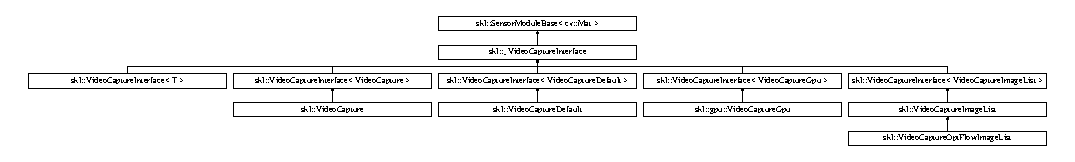
\includegraphics[height=1.733746cm]{classskl_1_1___video_capture_interface}
\end{center}
\end{figure}
\subsection*{Public Member Functions}
\begin{DoxyCompactItemize}
\item 
\hypertarget{classskl_1_1___video_capture_interface_a6212124bf4488c7b17255a2689a32d64}{}\label{classskl_1_1___video_capture_interface_a6212124bf4488c7b17255a2689a32d64} 
virtual bool {\bfseries open} (const std\+::string \&filename)=0
\item 
\hypertarget{classskl_1_1___video_capture_interface_a62596ea37320dd4790e5e37912c44cda}{}\label{classskl_1_1___video_capture_interface_a62596ea37320dd4790e5e37912c44cda} 
virtual bool {\bfseries open} (int device)=0
\item 
\hypertarget{classskl_1_1___video_capture_interface_a4130707d281129aa9eb648ac9b6b99d2}{}\label{classskl_1_1___video_capture_interface_a4130707d281129aa9eb648ac9b6b99d2} 
virtual bool {\bfseries is\+Opened} () const =0
\item 
\hypertarget{classskl_1_1___video_capture_interface_a9d3990d3cd85cbfbe70ce8d6565a3dea}{}\label{classskl_1_1___video_capture_interface_a9d3990d3cd85cbfbe70ce8d6565a3dea} 
virtual void \hyperlink{classskl_1_1___video_capture_interface_a9d3990d3cd85cbfbe70ce8d6565a3dea}{release} ()=0
\begin{DoxyCompactList}\small\item\em センサを特定する情報を入力する \end{DoxyCompactList}\item 
\hypertarget{classskl_1_1___video_capture_interface_a0dc57d91df8cee80a3e0c5cc09814ec1}{}\label{classskl_1_1___video_capture_interface_a0dc57d91df8cee80a3e0c5cc09814ec1} 
virtual bool {\bfseries grab} ()=0
\item 
\hypertarget{classskl_1_1___video_capture_interface_a915ccf5860023e3277abfd0c5d85eb14}{}\label{classskl_1_1___video_capture_interface_a915ccf5860023e3277abfd0c5d85eb14} 
virtual bool {\bfseries retrieve} (cv\+::\+Mat \&image, int channel=0)=0
\item 
\hypertarget{classskl_1_1___video_capture_interface_aef1026d5becac43d49f341dceff4440d}{}\label{classskl_1_1___video_capture_interface_aef1026d5becac43d49f341dceff4440d} 
size\+\_\+t {\bfseries size} () const
\item 
virtual bool \hyperlink{classskl_1_1___video_capture_interface_acf6bb54ae5d4bcee82029b36c8ae17bf}{is\+Pseudo\+Capture} () const
\item 
\hypertarget{classskl_1_1___video_capture_interface_a02ca8e0e253ee5f88cc5d078123d4caf}{}\label{classskl_1_1___video_capture_interface_a02ca8e0e253ee5f88cc5d078123d4caf} 
virtual bool \hyperlink{classskl_1_1___video_capture_interface_a02ca8e0e253ee5f88cc5d078123d4caf}{set} (capture\+\_\+property\+\_\+t prop\+\_\+id, double val)=0
\begin{DoxyCompactList}\small\item\em カメラに値やモード(camera\+\_\+mode\+\_\+tがset($\ast$,camera\+\_\+mode\+\_\+t mode)を通してvalに与えられる(modeは-\/4から-\/1までの整数)をセットする純粋仮想関数 \end{DoxyCompactList}\item 
\hypertarget{classskl_1_1___video_capture_interface_a9cb748d4cc424556936febfaaa74d9d8}{}\label{classskl_1_1___video_capture_interface_a9cb748d4cc424556936febfaaa74d9d8} 
virtual double \hyperlink{classskl_1_1___video_capture_interface_a9cb748d4cc424556936febfaaa74d9d8}{get} (capture\+\_\+property\+\_\+t prop\+\_\+id)=0
\begin{DoxyCompactList}\small\item\em カメラから値をgetする純粋仮想関数(modeはインターフェイス簡素化のためサポートしない) \end{DoxyCompactList}\item 
\hypertarget{classskl_1_1___video_capture_interface_a0a5b4a468dd49b004b9ccf087190e145}{}\label{classskl_1_1___video_capture_interface_a0a5b4a468dd49b004b9ccf087190e145} 
bool {\bfseries set} (const \hyperlink{classskl_1_1_video_capture_params}{Video\+Capture\+Params} \&params)
\item 
\hypertarget{classskl_1_1___video_capture_interface_a012ea0273c77069c70c8c2d8b2d1648d}{}\label{classskl_1_1___video_capture_interface_a012ea0273c77069c70c8c2d8b2d1648d} 
bool {\bfseries set} (const std\+::string \&prop\+\_\+name, double val)
\item 
\hypertarget{classskl_1_1___video_capture_interface_ad7e9069d5579b736e7b1088595ab12db}{}\label{classskl_1_1___video_capture_interface_ad7e9069d5579b736e7b1088595ab12db} 
bool {\bfseries set} (const std\+::string \&prop\+\_\+name, camera\+\_\+mode\+\_\+t mode)
\item 
\hypertarget{classskl_1_1___video_capture_interface_a5ed9bbd7ac6450a5d343e1c24c7f0ed7}{}\label{classskl_1_1___video_capture_interface_a5ed9bbd7ac6450a5d343e1c24c7f0ed7} 
bool {\bfseries set} (capture\+\_\+property\+\_\+t prop\+\_\+id, camera\+\_\+mode\+\_\+t mode)
\item 
\hypertarget{classskl_1_1___video_capture_interface_ae8521689d8536434e121ffcaf42a2653}{}\label{classskl_1_1___video_capture_interface_ae8521689d8536434e121ffcaf42a2653} 
const \hyperlink{classskl_1_1_video_capture_params}{Video\+Capture\+Params} \& {\bfseries get} ()
\item 
\hypertarget{classskl_1_1___video_capture_interface_a3ab336503077b3567c56fbe3f0d2dbaa}{}\label{classskl_1_1___video_capture_interface_a3ab336503077b3567c56fbe3f0d2dbaa} 
double {\bfseries get} (const std\+::string \&prop\+\_\+name)
\end{DoxyCompactItemize}
\subsection*{Protected Attributes}
\begin{DoxyCompactItemize}
\item 
\hypertarget{classskl_1_1___video_capture_interface_ad1732916c33a970c2a5c0fa12698f4ab}{}\label{classskl_1_1___video_capture_interface_ad1732916c33a970c2a5c0fa12698f4ab} 
\hyperlink{classskl_1_1_video_capture_params}{Video\+Capture\+Params} {\bfseries params}
\end{DoxyCompactItemize}


\subsection{Detailed Description}
S\+K\+Lにおける\+Video\+Capture用のインターフェイス  実際に\+Video\+Captureを作るときには,この後で宣言されているoperator$<$$<$を持ったテンプレートつきインターフェイス\+Video\+Capture$<$\+T$>$を継承すること 

\subsection{Member Function Documentation}
\hypertarget{classskl_1_1___video_capture_interface_acf6bb54ae5d4bcee82029b36c8ae17bf}{}\label{classskl_1_1___video_capture_interface_acf6bb54ae5d4bcee82029b36c8ae17bf} 
\index{skl\+::\+\_\+\+Video\+Capture\+Interface@{skl\+::\+\_\+\+Video\+Capture\+Interface}!is\+Pseudo\+Capture@{is\+Pseudo\+Capture}}
\index{is\+Pseudo\+Capture@{is\+Pseudo\+Capture}!skl\+::\+\_\+\+Video\+Capture\+Interface@{skl\+::\+\_\+\+Video\+Capture\+Interface}}
\subsubsection{\texorpdfstring{is\+Pseudo\+Capture()}{isPseudoCapture()}}
{\footnotesize\ttfamily virtual bool skl\+::\+\_\+\+Video\+Capture\+Interface\+::is\+Pseudo\+Capture (\begin{DoxyParamCaption}{ }\end{DoxyParamCaption}) const\hspace{0.3cm}{\ttfamily [inline]}, {\ttfamily [virtual]}}

本来は取得データがないのに補間したデータなどを利用している 場合にtrueとなる。具象クラスで特に実装がなければfalseを返す 

The documentation for this class was generated from the following files\+:\begin{DoxyCompactItemize}
\item 
Open\+C\+V/include/\hyperlink{_video_capture_interface_8h}{Video\+Capture\+Interface.\+h}\item 
Open\+C\+V/src/\hyperlink{_video_capture_interface_8cpp}{Video\+Capture\+Interface.\+cpp}\end{DoxyCompactItemize}

\hypertarget{classskl_1_1_background_subtract_algorithm}{}\section{skl\+:\+:Background\+Subtract\+Algorithm Class Reference}
\label{classskl_1_1_background_subtract_algorithm}\index{skl\+::\+Background\+Subtract\+Algorithm@{skl\+::\+Background\+Subtract\+Algorithm}}
Inheritance diagram for skl\+:\+:Background\+Subtract\+Algorithm\+:\begin{figure}[H]
\begin{center}
\leavevmode
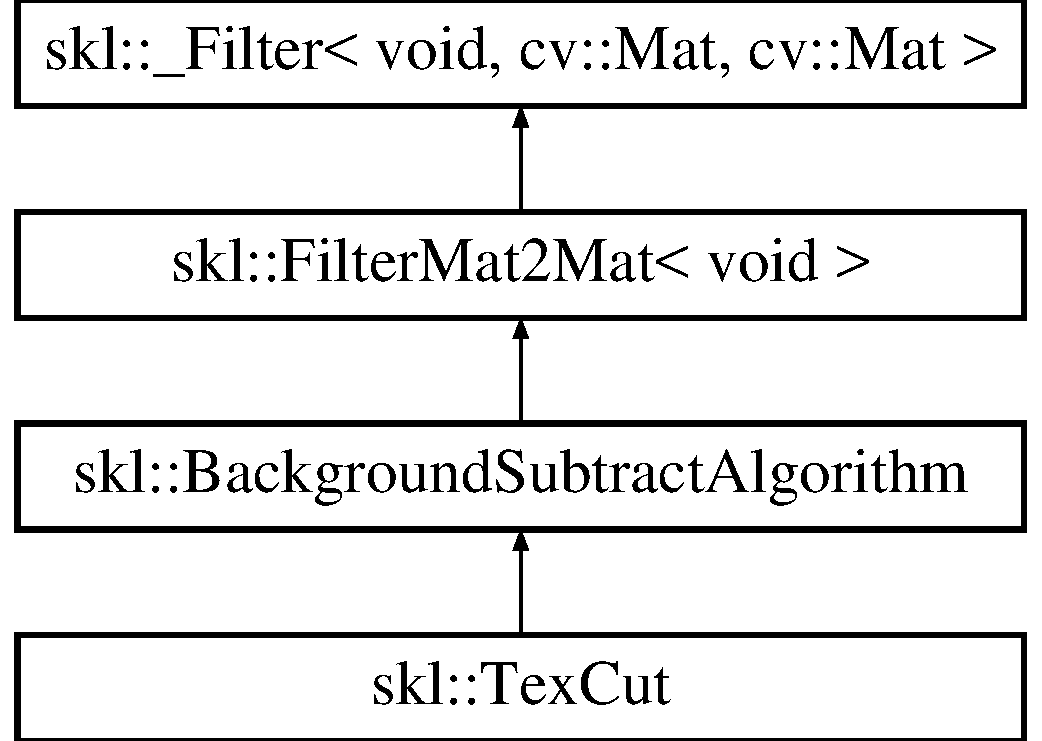
\includegraphics[height=4.000000cm]{classskl_1_1_background_subtract_algorithm}
\end{center}
\end{figure}
\subsection*{Public Member Functions}
\begin{DoxyCompactItemize}
\item 
\hypertarget{classskl_1_1_background_subtract_algorithm_a7668b90a228834226c6a8b4455b7d90d}{}\label{classskl_1_1_background_subtract_algorithm_a7668b90a228834226c6a8b4455b7d90d} 
virtual void {\bfseries compute} (const cv\+::\+Mat \&src, cv\+::\+Mat \&dest)
\item 
\hypertarget{classskl_1_1_background_subtract_algorithm_abb85a3bca26d5d3c068c64ac23be357e}{}\label{classskl_1_1_background_subtract_algorithm_abb85a3bca26d5d3c068c64ac23be357e} 
virtual void {\bfseries compute} (const cv\+::\+Mat \&src, const cv\+::\+Mat \&mask, cv\+::\+Mat \&dest)=0
\item 
\hypertarget{classskl_1_1_background_subtract_algorithm_a47674198d79e2394d072ffa5a2a74d0a}{}\label{classskl_1_1_background_subtract_algorithm_a47674198d79e2394d072ffa5a2a74d0a} 
virtual cv\+::\+Mat {\bfseries background} () const =0
\item 
\hypertarget{classskl_1_1_background_subtract_algorithm_aefe8422738decfcfb16ea8d7ea69c7c1}{}\label{classskl_1_1_background_subtract_algorithm_aefe8422738decfcfb16ea8d7ea69c7c1} 
virtual void {\bfseries update\+Background\+Model} (const cv\+::\+Mat \&img)=0
\end{DoxyCompactItemize}


The documentation for this class was generated from the following files\+:\begin{DoxyCompactItemize}
\item 
Open\+C\+V/include/Background\+Subtract\+Algorithm.\+h\item 
Open\+C\+V/src/Background\+Subtract\+Algorithm.\+cpp\end{DoxyCompactItemize}

\hypertarget{classbg__update__parallel}{}\section{bg\+\_\+update\+\_\+parallel Class Reference}
\label{classbg__update__parallel}\index{bg\+\_\+update\+\_\+parallel@{bg\+\_\+update\+\_\+parallel}}
\subsection*{Public Member Functions}
\begin{DoxyCompactItemize}
\item 
\hypertarget{classbg__update__parallel_aa7f19f05768b79cdfd963a4fff18e315}{}\label{classbg__update__parallel_aa7f19f05768b79cdfd963a4fff18e315} 
{\bfseries bg\+\_\+update\+\_\+parallel} (const cv\+::\+Mat \&src, cv\+::\+Mat \&bg1, cv\+::\+Mat \&bg2, const cv\+::\+Mat \&non\+\_\+update\+\_\+mask, const cv\+::\+Mat \&no\+\_\+touch\+\_\+fg, float \+\_\+learning\+\_\+rate, float \+\_\+learning\+\_\+rate2)
\item 
\hypertarget{classbg__update__parallel_afe8c47ecac8fb0b4af9ed0e4e4689cda}{}\label{classbg__update__parallel_afe8c47ecac8fb0b4af9ed0e4e4689cda} 
void {\bfseries operator()} (const cv\+::\+Blocked\+Range \&range) const
\item 
\hypertarget{classbg__update__parallel_aa7f19f05768b79cdfd963a4fff18e315}{}\label{classbg__update__parallel_aa7f19f05768b79cdfd963a4fff18e315} 
{\bfseries bg\+\_\+update\+\_\+parallel} (const cv\+::\+Mat \&src, cv\+::\+Mat \&bg1, cv\+::\+Mat \&bg2, const cv\+::\+Mat \&non\+\_\+update\+\_\+mask, const cv\+::\+Mat \&no\+\_\+touch\+\_\+fg, float \+\_\+learning\+\_\+rate, float \+\_\+learning\+\_\+rate2)
\item 
\hypertarget{classbg__update__parallel_afe8c47ecac8fb0b4af9ed0e4e4689cda}{}\label{classbg__update__parallel_afe8c47ecac8fb0b4af9ed0e4e4689cda} 
void {\bfseries operator()} (const cv\+::\+Blocked\+Range \&range) const
\end{DoxyCompactItemize}
\subsection*{Protected Attributes}
\begin{DoxyCompactItemize}
\item 
\hypertarget{classbg__update__parallel_ae1c3e97ab55c49abeeb39e6db59e9c85}{}\label{classbg__update__parallel_ae1c3e97ab55c49abeeb39e6db59e9c85} 
const cv\+::\+Mat \& {\bfseries src}
\item 
\hypertarget{classbg__update__parallel_af1160d47a07171184c8d0fe00b9e17b3}{}\label{classbg__update__parallel_af1160d47a07171184c8d0fe00b9e17b3} 
cv\+::\+Mat \& {\bfseries bg1}
\item 
\hypertarget{classbg__update__parallel_a595c319c1e73500138446fa658f1ea3e}{}\label{classbg__update__parallel_a595c319c1e73500138446fa658f1ea3e} 
cv\+::\+Mat \& {\bfseries bg2}
\item 
\hypertarget{classbg__update__parallel_a09df8634dd493bf9c2b6dc6d0e8059d5}{}\label{classbg__update__parallel_a09df8634dd493bf9c2b6dc6d0e8059d5} 
const cv\+::\+Mat \& {\bfseries non\+\_\+update\+\_\+mask}
\item 
\hypertarget{classbg__update__parallel_a87a1f23081a7686dfac2cf93d1f51dd4}{}\label{classbg__update__parallel_a87a1f23081a7686dfac2cf93d1f51dd4} 
const cv\+::\+Mat \& {\bfseries no\+\_\+touch\+\_\+fg}
\item 
\hypertarget{classbg__update__parallel_a476b5920c0c278c10c04672a152ca9a4}{}\label{classbg__update__parallel_a476b5920c0c278c10c04672a152ca9a4} 
float {\bfseries \+\_\+learning\+\_\+rate}
\item 
\hypertarget{classbg__update__parallel_a14e2818a8876a20b7036f2c1ffa908bf}{}\label{classbg__update__parallel_a14e2818a8876a20b7036f2c1ffa908bf} 
float {\bfseries \+\_\+learning\+\_\+rate2}
\end{DoxyCompactItemize}


The documentation for this class was generated from the following file\+:\begin{DoxyCompactItemize}
\item 
Open\+C\+V/src/Table\+Object\+Manager\+Bi\+Background.\+cpp\end{DoxyCompactItemize}

\hypertarget{classskl_1_1_chiffon_base}{}\section{skl\+:\+:Chiffon\+Base Class Reference}
\label{classskl_1_1_chiffon_base}\index{skl\+::\+Chiffon\+Base@{skl\+::\+Chiffon\+Base}}


Chiffon\+Vieer/\+Navigator共通の処理を記述するインターフェイス   




{\ttfamily \#include $<$Chiffon\+Base.\+h$>$}

Inheritance diagram for skl\+:\+:Chiffon\+Base\+:\begin{figure}[H]
\begin{center}
\leavevmode
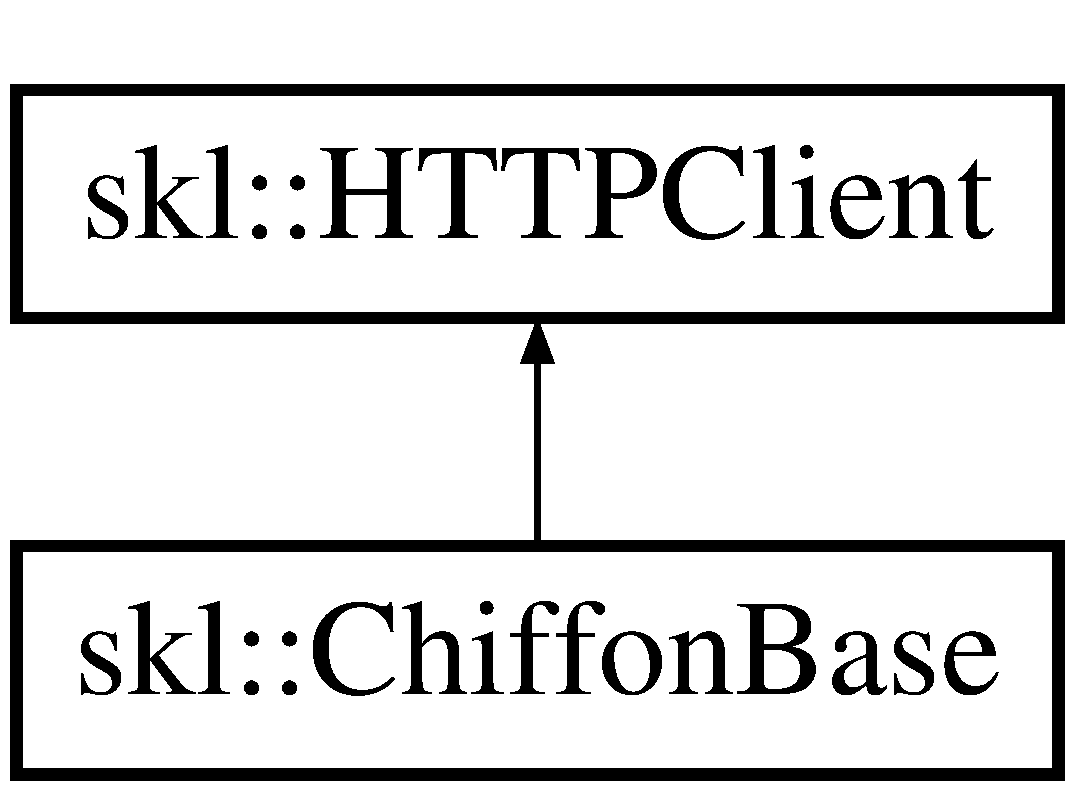
\includegraphics[height=2.000000cm]{classskl_1_1_chiffon_base}
\end{center}
\end{figure}
\subsection*{Public Member Functions}
\begin{DoxyCompactItemize}
\item 
\hypertarget{classskl_1_1_chiffon_base_ad52ce5895d15a9c1b16419f09e9b4d36}{}\label{classskl_1_1_chiffon_base_ad52ce5895d15a9c1b16419f09e9b4d36} 
\hyperlink{classskl_1_1_chiffon_base_ad52ce5895d15a9c1b16419f09e9b4d36}{Chiffon\+Base} (const std\+::string \&host, int port)
\begin{DoxyCompactList}\small\item\em デフォルトコンストラクタ \end{DoxyCompactList}\item 
\hypertarget{classskl_1_1_chiffon_base_ae1a4691bb4aad50ebcc3899aae8d3c00}{}\label{classskl_1_1_chiffon_base_ae1a4691bb4aad50ebcc3899aae8d3c00} 
virtual \hyperlink{classskl_1_1_chiffon_base_ae1a4691bb4aad50ebcc3899aae8d3c00}{$\sim$\+Chiffon\+Base} ()
\begin{DoxyCompactList}\small\item\em デストラクタ \end{DoxyCompactList}\end{DoxyCompactItemize}
\subsection*{Protected Member Functions}
\begin{DoxyCompactItemize}
\item 
\hypertarget{classskl_1_1_chiffon_base_aac461d11065188b07c1c3aa73ef70368}{}\label{classskl_1_1_chiffon_base_aac461d11065188b07c1c3aa73ef70368} 
bool {\bfseries get} (const std\+::string \&path, const picojson\+::value \&query)
\item 
\hypertarget{classskl_1_1_chiffon_base_aad2939076444319328aff4e3b71e2a46}{}\label{classskl_1_1_chiffon_base_aad2939076444319328aff4e3b71e2a46} 
bool {\bfseries post} (const std\+::string \&path, const picojson\+::value \&query)
\end{DoxyCompactItemize}
\subsection*{Additional Inherited Members}


\subsection{Detailed Description}
Chiffon\+Vieer/\+Navigator共通の処理を記述するインターフェイス  

The documentation for this class was generated from the following files\+:\begin{DoxyCompactItemize}
\item 
Core/include/\hyperlink{_chiffon_base_8h}{Chiffon\+Base.\+h}\item 
Core/src/\hyperlink{_chiffon_base_8cpp}{Chiffon\+Base.\+cpp}\end{DoxyCompactItemize}

\hypertarget{classskl_1_1_comparable}{}\section{skl\+:\+:Comparable$<$ T $>$ Class Template Reference}
\label{classskl_1_1_comparable}\index{skl\+::\+Comparable$<$ T $>$@{skl\+::\+Comparable$<$ T $>$}}


比較可能なオブジェクトであることを示す(operator$<$を定義するだけで他の比較演算子が出来る)  




{\ttfamily \#include $<$Comparable.\+h$>$}

Inheritance diagram for skl\+:\+:Comparable$<$ T $>$\+:\begin{figure}[H]
\begin{center}
\leavevmode
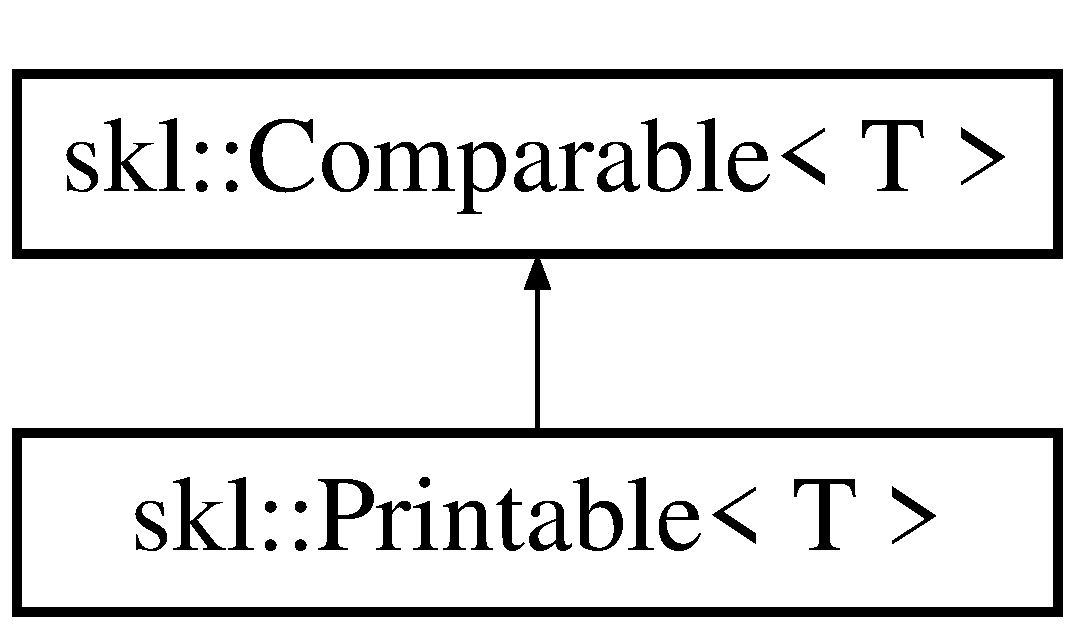
\includegraphics[height=2.000000cm]{classskl_1_1_comparable}
\end{center}
\end{figure}
\subsection*{Public Member Functions}
\begin{DoxyCompactItemize}
\item 
\hypertarget{classskl_1_1_comparable_a08ded8ee95f5d2453106761b984dad50}{}\label{classskl_1_1_comparable_a08ded8ee95f5d2453106761b984dad50} 
virtual bool {\bfseries operator$<$} (const T \&other) const =0
\end{DoxyCompactItemize}
\subsection*{Friends}
\begin{DoxyCompactItemize}
\item 
\hypertarget{classskl_1_1_comparable_a2cde4518a54e4900eac612f536e5303e}{}\label{classskl_1_1_comparable_a2cde4518a54e4900eac612f536e5303e} 
bool {\bfseries operator$>$=} (const T \&lhs, const T \&rhs)
\item 
\hypertarget{classskl_1_1_comparable_a55af6cb1ca766f6fba5fe1a6ff3d7b54}{}\label{classskl_1_1_comparable_a55af6cb1ca766f6fba5fe1a6ff3d7b54} 
bool {\bfseries operator$>$} (const T \&lhs, const T \&rhs)
\item 
\hypertarget{classskl_1_1_comparable_a3c5ac45ccee4dd4a74a67e6886309072}{}\label{classskl_1_1_comparable_a3c5ac45ccee4dd4a74a67e6886309072} 
bool {\bfseries operator$<$=} (const T \&lhs, const T \&rhs)
\item 
\hypertarget{classskl_1_1_comparable_aa9434de986958333c8a4114e04b83f1a}{}\label{classskl_1_1_comparable_aa9434de986958333c8a4114e04b83f1a} 
bool {\bfseries operator!=} (const T \&lhs, const T \&rhs)
\item 
\hypertarget{classskl_1_1_comparable_ae55aaa8ab31c31ebc41b762886835b05}{}\label{classskl_1_1_comparable_ae55aaa8ab31c31ebc41b762886835b05} 
bool {\bfseries operator==} (const T \&lhs, const T \&rhs)
\end{DoxyCompactItemize}


\subsection{Detailed Description}
\subsubsection*{template$<$class T$>$\newline
class skl\+::\+Comparable$<$ T $>$}

比較可能なオブジェクトであることを示す(operator$<$を定義するだけで他の比較演算子が出来る) 

The documentation for this class was generated from the following file\+:\begin{DoxyCompactItemize}
\item 
Core/include/\hyperlink{_comparable_8h}{Comparable.\+h}\end{DoxyCompactItemize}

\hypertarget{classskl_1_1_count_moving_pixels}{}\section{skl\+:\+:Count\+Moving\+Pixels Class Reference}
\label{classskl_1_1_count_moving_pixels}\index{skl\+::\+Count\+Moving\+Pixels@{skl\+::\+Count\+Moving\+Pixels}}
\subsection*{Public Member Functions}
\begin{DoxyCompactItemize}
\item 
\hypertarget{classskl_1_1_count_moving_pixels_a2d5f19e230ff2bec120df5996374869f}{}\label{classskl_1_1_count_moving_pixels_a2d5f19e230ff2bec120df5996374869f} 
\hyperlink{classskl_1_1_count_moving_pixels_a2d5f19e230ff2bec120df5996374869f}{Count\+Moving\+Pixels} (float thresh, int step, int life=2, bool shallow\+\_\+copy=false)
\begin{DoxyCompactList}\small\item\em デフォルトコンストラクタ \end{DoxyCompactList}\item 
\hypertarget{classskl_1_1_count_moving_pixels_a2dcd33080fad0140b763be8aded3f993}{}\label{classskl_1_1_count_moving_pixels_a2dcd33080fad0140b763be8aded3f993} 
virtual \hyperlink{classskl_1_1_count_moving_pixels_a2dcd33080fad0140b763be8aded3f993}{$\sim$\+Count\+Moving\+Pixels} ()
\begin{DoxyCompactList}\small\item\em デストラクタ \end{DoxyCompactList}\item 
\hypertarget{classskl_1_1_count_moving_pixels_afb1aa1df8ac9fcdc9c3f39d028aee762}{}\label{classskl_1_1_count_moving_pixels_afb1aa1df8ac9fcdc9c3f39d028aee762} 
virtual float {\bfseries compute} (const cv\+::\+Mat \&img)
\item 
\hypertarget{classskl_1_1_count_moving_pixels_ac0a55bad93f0a733ea859e21f7715102}{}\label{classskl_1_1_count_moving_pixels_ac0a55bad93f0a733ea859e21f7715102} 
float {\bfseries thresh} () const
\item 
\hypertarget{classskl_1_1_count_moving_pixels_af5e555709b161a5b8ac46dce1da7d467}{}\label{classskl_1_1_count_moving_pixels_af5e555709b161a5b8ac46dce1da7d467} 
void {\bfseries thresh} (float \+\_\+\+\_\+thresh)
\item 
\hypertarget{classskl_1_1_count_moving_pixels_a0bf84f91adb4d6b39330ee9469a9be00}{}\label{classskl_1_1_count_moving_pixels_a0bf84f91adb4d6b39330ee9469a9be00} 
int {\bfseries step} () const
\item 
\hypertarget{classskl_1_1_count_moving_pixels_a53cb9cc391d39c60a1de41c8ef27d283}{}\label{classskl_1_1_count_moving_pixels_a53cb9cc391d39c60a1de41c8ef27d283} 
void {\bfseries step} (int \+\_\+\+\_\+step)
\item 
\hypertarget{classskl_1_1_count_moving_pixels_a5f27cafa0f77b9476350ef2b14e9cdfd}{}\label{classskl_1_1_count_moving_pixels_a5f27cafa0f77b9476350ef2b14e9cdfd} 
bool {\bfseries shallow\+\_\+copy} () const
\item 
\hypertarget{classskl_1_1_count_moving_pixels_abcce3c874bc643cc301d62b1b8312b64}{}\label{classskl_1_1_count_moving_pixels_abcce3c874bc643cc301d62b1b8312b64} 
void {\bfseries shallow\+\_\+copy} (bool \+\_\+\+\_\+shallow\+\_\+copy)
\end{DoxyCompactItemize}
\subsection*{Protected Attributes}
\begin{DoxyCompactItemize}
\item 
\hypertarget{classskl_1_1_count_moving_pixels_aa663a7380267baef4f53dc10a218bc85}{}\label{classskl_1_1_count_moving_pixels_aa663a7380267baef4f53dc10a218bc85} 
float {\bfseries \+\_\+thresh}
\item 
\hypertarget{classskl_1_1_count_moving_pixels_a4ff07f9308bbbe59bf8b163b2c887702}{}\label{classskl_1_1_count_moving_pixels_a4ff07f9308bbbe59bf8b163b2c887702} 
int {\bfseries \+\_\+step}
\item 
\hypertarget{classskl_1_1_count_moving_pixels_a9f5d47fff1f077d7408f288fc8d77f8e}{}\label{classskl_1_1_count_moving_pixels_a9f5d47fff1f077d7408f288fc8d77f8e} 
bool {\bfseries \+\_\+shallow\+\_\+copy}
\item 
\hypertarget{classskl_1_1_count_moving_pixels_aaa51878cf7966d53ecdca9d15e4f92d9}{}\label{classskl_1_1_count_moving_pixels_aaa51878cf7966d53ecdca9d15e4f92d9} 
std\+::vector$<$ cv\+::\+Mat $>$ {\bfseries prevs}
\item 
\hypertarget{classskl_1_1_count_moving_pixels_a85b30818c6ebdb77ba0bb9cae60dae41}{}\label{classskl_1_1_count_moving_pixels_a85b30818c6ebdb77ba0bb9cae60dae41} 
size\+\_\+t {\bfseries phase}
\end{DoxyCompactItemize}


The documentation for this class was generated from the following files\+:\begin{DoxyCompactItemize}
\item 
Open\+C\+V/include/Count\+Moving\+Pixels.\+h\item 
Open\+C\+V/src/\hyperlink{_count_moving_pixels_8cpp}{Count\+Moving\+Pixels.\+cpp}\end{DoxyCompactItemize}

\hypertarget{classskl_1_1_cv_mouse_event_handler}{}\section{skl\+:\+:Cv\+Mouse\+Event\+Handler Class Reference}
\label{classskl_1_1_cv_mouse_event_handler}\index{skl\+::\+Cv\+Mouse\+Event\+Handler@{skl\+::\+Cv\+Mouse\+Event\+Handler}}
\subsection*{Public Member Functions}
\begin{DoxyCompactItemize}
\item 
\hypertarget{classskl_1_1_cv_mouse_event_handler_ae611ebdede7117727dab439549daee56}{}\label{classskl_1_1_cv_mouse_event_handler_ae611ebdede7117727dab439549daee56} 
\hyperlink{classskl_1_1_cv_mouse_event_handler_ae611ebdede7117727dab439549daee56}{Cv\+Mouse\+Event\+Handler} (const std\+::string \&window\+\_\+name)
\begin{DoxyCompactList}\small\item\em コンストラクタ \end{DoxyCompactList}\item 
\hypertarget{classskl_1_1_cv_mouse_event_handler_a294d6b2bcec7fed58870490a9a7b1c57}{}\label{classskl_1_1_cv_mouse_event_handler_a294d6b2bcec7fed58870490a9a7b1c57} 
\hyperlink{classskl_1_1_cv_mouse_event_handler_a294d6b2bcec7fed58870490a9a7b1c57}{$\sim$\+Cv\+Mouse\+Event\+Handler} ()
\begin{DoxyCompactList}\small\item\em デストラクタ \end{DoxyCompactList}\item 
\hypertarget{classskl_1_1_cv_mouse_event_handler_a989c07ba1c82349a31d1bf6f6fa9ec9b}{}\label{classskl_1_1_cv_mouse_event_handler_a989c07ba1c82349a31d1bf6f6fa9ec9b} 
cv\+::\+Point {\bfseries location} () const
\item 
\hypertarget{classskl_1_1_cv_mouse_event_handler_a9b1982af63fae7634b791453034053dd}{}\label{classskl_1_1_cv_mouse_event_handler_a9b1982af63fae7634b791453034053dd} 
int {\bfseries flag} () const
\item 
\hypertarget{classskl_1_1_cv_mouse_event_handler_afeb529fb49664cad1134dd4812ea810d}{}\label{classskl_1_1_cv_mouse_event_handler_afeb529fb49664cad1134dd4812ea810d} 
std\+::queue$<$ \hyperlink{structskl_1_1_mouse_event}{Mouse\+Event} $>$ \& {\bfseries events} ()
\end{DoxyCompactItemize}
\subsection*{Protected Attributes}
\begin{DoxyCompactItemize}
\item 
\hypertarget{classskl_1_1_cv_mouse_event_handler_a1362364b6f62514a5517bab7dafd5d40}{}\label{classskl_1_1_cv_mouse_event_handler_a1362364b6f62514a5517bab7dafd5d40} 
cv\+::\+Point {\bfseries \+\_\+location}
\item 
\hypertarget{classskl_1_1_cv_mouse_event_handler_aaa1f14b43bfaf39760edd7ad6a73f46f}{}\label{classskl_1_1_cv_mouse_event_handler_aaa1f14b43bfaf39760edd7ad6a73f46f} 
int {\bfseries \+\_\+flag}
\item 
\hypertarget{classskl_1_1_cv_mouse_event_handler_aedbff79ce36f31e7f4d74ea600df9864}{}\label{classskl_1_1_cv_mouse_event_handler_aedbff79ce36f31e7f4d74ea600df9864} 
std\+::queue$<$ \hyperlink{structskl_1_1_mouse_event}{Mouse\+Event} $>$ {\bfseries \+\_\+events}
\end{DoxyCompactItemize}


The documentation for this class was generated from the following files\+:\begin{DoxyCompactItemize}
\item 
Open\+C\+V/include/\hyperlink{_cv_mouse_event_handler_8h}{Cv\+Mouse\+Event\+Handler.\+h}\item 
Open\+C\+V/src/\hyperlink{_cv_mouse_event_handler_8cpp}{Cv\+Mouse\+Event\+Handler.\+cpp}\end{DoxyCompactItemize}

\hypertarget{classskl_1_1gpu_1_1_filter_gpu_mat2_gpu_mat}{}\section{skl\+:\+:gpu\+:\+:Filter\+Gpu\+Mat2\+Gpu\+Mat$<$ R\+ET $>$ Class Template Reference}
\label{classskl_1_1gpu_1_1_filter_gpu_mat2_gpu_mat}\index{skl\+::gpu\+::\+Filter\+Gpu\+Mat2\+Gpu\+Mat$<$ R\+E\+T $>$@{skl\+::gpu\+::\+Filter\+Gpu\+Mat2\+Gpu\+Mat$<$ R\+E\+T $>$}}


cv\+::gpu\+::\+Gpu\+Matを引数としてとる\+Filter  




{\ttfamily \#include $<$Filter\+Gpu\+Mat2\+Gpu\+Mat.\+h$>$}

Inheritance diagram for skl\+:\+:gpu\+:\+:Filter\+Gpu\+Mat2\+Gpu\+Mat$<$ R\+ET $>$\+:\begin{figure}[H]
\begin{center}
\leavevmode
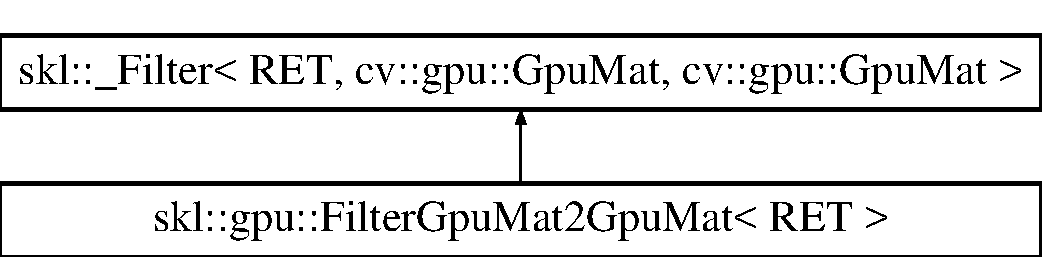
\includegraphics[height=2.000000cm]{classskl_1_1gpu_1_1_filter_gpu_mat2_gpu_mat}
\end{center}
\end{figure}
\subsection*{Public Member Functions}
\begin{DoxyCompactItemize}
\item 
\hypertarget{classskl_1_1gpu_1_1_filter_gpu_mat2_gpu_mat_a0189451d4a1cdf732b527baec5ec3419}{}\label{classskl_1_1gpu_1_1_filter_gpu_mat2_gpu_mat_a0189451d4a1cdf732b527baec5ec3419} 
virtual R\+ET {\bfseries compute} (const cv\+::gpu\+::\+Gpu\+Mat \&src, cv\+::gpu\+::\+Gpu\+Mat \&dest)
\item 
\hypertarget{classskl_1_1gpu_1_1_filter_gpu_mat2_gpu_mat_a86966fac0c2622d3856671f167a5fa7b}{}\label{classskl_1_1gpu_1_1_filter_gpu_mat2_gpu_mat_a86966fac0c2622d3856671f167a5fa7b} 
virtual R\+ET {\bfseries compute} (const cv\+::gpu\+::\+Gpu\+Mat \&src, cv\+::gpu\+::\+Gpu\+Mat \&dest, cv\+::gpu\+::\+Stream \&s)=0
\item 
\hypertarget{classskl_1_1gpu_1_1_filter_gpu_mat2_gpu_mat_a85d4ba1e609b020fa3a27d540b0d9915}{}\label{classskl_1_1gpu_1_1_filter_gpu_mat2_gpu_mat_a85d4ba1e609b020fa3a27d540b0d9915} 
virtual R\+ET {\bfseries compute} (const cv\+::\+Mat \&src, cv\+::\+Mat \&dest, cv\+::gpu\+::\+Stream \&s=cv\+::gpu\+::\+Stream\+::\+Null())
\item 
\hypertarget{classskl_1_1gpu_1_1_filter_gpu_mat2_gpu_mat_acff099208f52a6a0da328d1b9e02b711}{}\label{classskl_1_1gpu_1_1_filter_gpu_mat2_gpu_mat_acff099208f52a6a0da328d1b9e02b711} 
virtual R\+ET {\bfseries compute} (const cv\+::\+Mat \&src, cv\+::gpu\+::\+Gpu\+Mat \&dest, cv\+::gpu\+::\+Stream \&s=cv\+::gpu\+::\+Stream\+::\+Null())
\item 
\hypertarget{classskl_1_1gpu_1_1_filter_gpu_mat2_gpu_mat_a874f7fcf98ec9ab35cd0529d53b1d80f}{}\label{classskl_1_1gpu_1_1_filter_gpu_mat2_gpu_mat_a874f7fcf98ec9ab35cd0529d53b1d80f} 
virtual R\+ET {\bfseries compute} (const cv\+::gpu\+::\+Gpu\+Mat \&src, cv\+::\+Mat \&dest, cv\+::gpu\+::\+Stream \&s=cv\+::gpu\+::\+Stream\+::\+Null())
\end{DoxyCompactItemize}
\subsection*{Protected Attributes}
\begin{DoxyCompactItemize}
\item 
\hypertarget{classskl_1_1gpu_1_1_filter_gpu_mat2_gpu_mat_a8b15362578aa443b6ccbb809cf4c2437}{}\label{classskl_1_1gpu_1_1_filter_gpu_mat2_gpu_mat_a8b15362578aa443b6ccbb809cf4c2437} 
cv\+::gpu\+::\+Gpu\+Mat {\bfseries src\+\_\+buf}
\item 
\hypertarget{classskl_1_1gpu_1_1_filter_gpu_mat2_gpu_mat_a0f2b8b38655cb0aaf695e7b58f67b49b}{}\label{classskl_1_1gpu_1_1_filter_gpu_mat2_gpu_mat_a0f2b8b38655cb0aaf695e7b58f67b49b} 
cv\+::gpu\+::\+Gpu\+Mat {\bfseries dest\+\_\+buf}
\end{DoxyCompactItemize}


\subsection{Detailed Description}
\subsubsection*{template$<$class R\+ET = bool$>$\newline
class skl\+::gpu\+::\+Filter\+Gpu\+Mat2\+Gpu\+Mat$<$ R\+E\+T $>$}

cv\+::gpu\+::\+Gpu\+Matを引数としてとる\+Filter 

The documentation for this class was generated from the following file\+:\begin{DoxyCompactItemize}
\item 
Open\+C\+V\+G\+P\+U/include/\hyperlink{_filter_gpu_mat2_gpu_mat_8h}{Filter\+Gpu\+Mat2\+Gpu\+Mat.\+h}\end{DoxyCompactItemize}

\hypertarget{classskl_1_1_filter_mat2_mat}{}\section{skl\+:\+:Filter\+Mat2\+Mat$<$ T $>$ Class Template Reference}
\label{classskl_1_1_filter_mat2_mat}\index{skl\+::\+Filter\+Mat2\+Mat$<$ T $>$@{skl\+::\+Filter\+Mat2\+Mat$<$ T $>$}}
Inheritance diagram for skl\+:\+:Filter\+Mat2\+Mat$<$ T $>$\+:\begin{figure}[H]
\begin{center}
\leavevmode
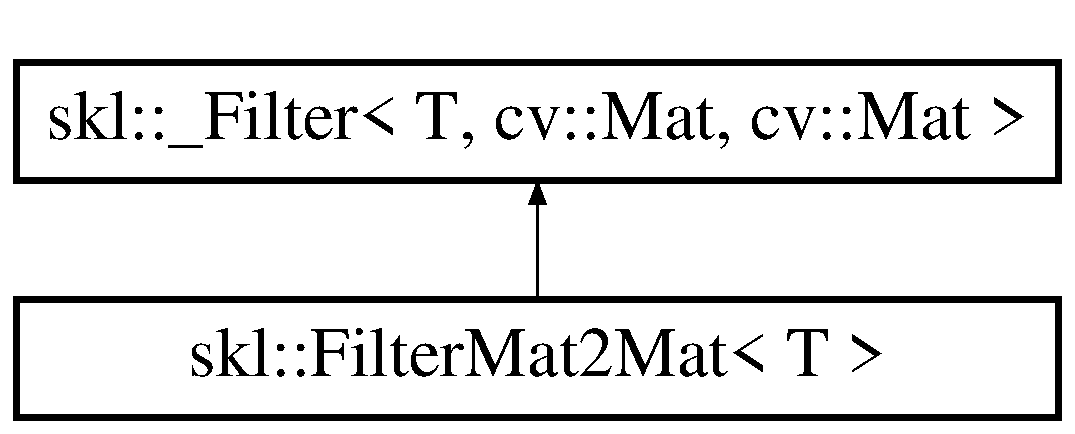
\includegraphics[height=2.000000cm]{classskl_1_1_filter_mat2_mat}
\end{center}
\end{figure}
\subsection*{Public Member Functions}
\begin{DoxyCompactItemize}
\item 
\hypertarget{classskl_1_1_filter_mat2_mat_ad906b4418761b1ba3a8ac446e53b4313}{}\label{classskl_1_1_filter_mat2_mat_ad906b4418761b1ba3a8ac446e53b4313} 
virtual T {\bfseries compute} (const cv\+::\+Mat \&src, cv\+::\+Mat \&dest)
\item 
\hypertarget{classskl_1_1_filter_mat2_mat_a5e86d618516207e937bf6f3c72fc3324}{}\label{classskl_1_1_filter_mat2_mat_a5e86d618516207e937bf6f3c72fc3324} 
virtual T {\bfseries compute} (const cv\+::\+Mat \&src, const cv\+::\+Mat \&mask, cv\+::\+Mat \&dest)=0
\end{DoxyCompactItemize}


The documentation for this class was generated from the following file\+:\begin{DoxyCompactItemize}
\item 
Open\+C\+V/include/Filter\+Mat2\+Mat.\+h\end{DoxyCompactItemize}

\hypertarget{classskl_1_1_flow}{}\section{skl\+:\+:Flow Class Reference}
\label{classskl_1_1_flow}\index{skl\+::\+Flow@{skl\+::\+Flow}}


Class for optical flow.  




{\ttfamily \#include $<$Flow.\+h$>$}

Inheritance diagram for skl\+:\+:Flow\+:\begin{figure}[H]
\begin{center}
\leavevmode
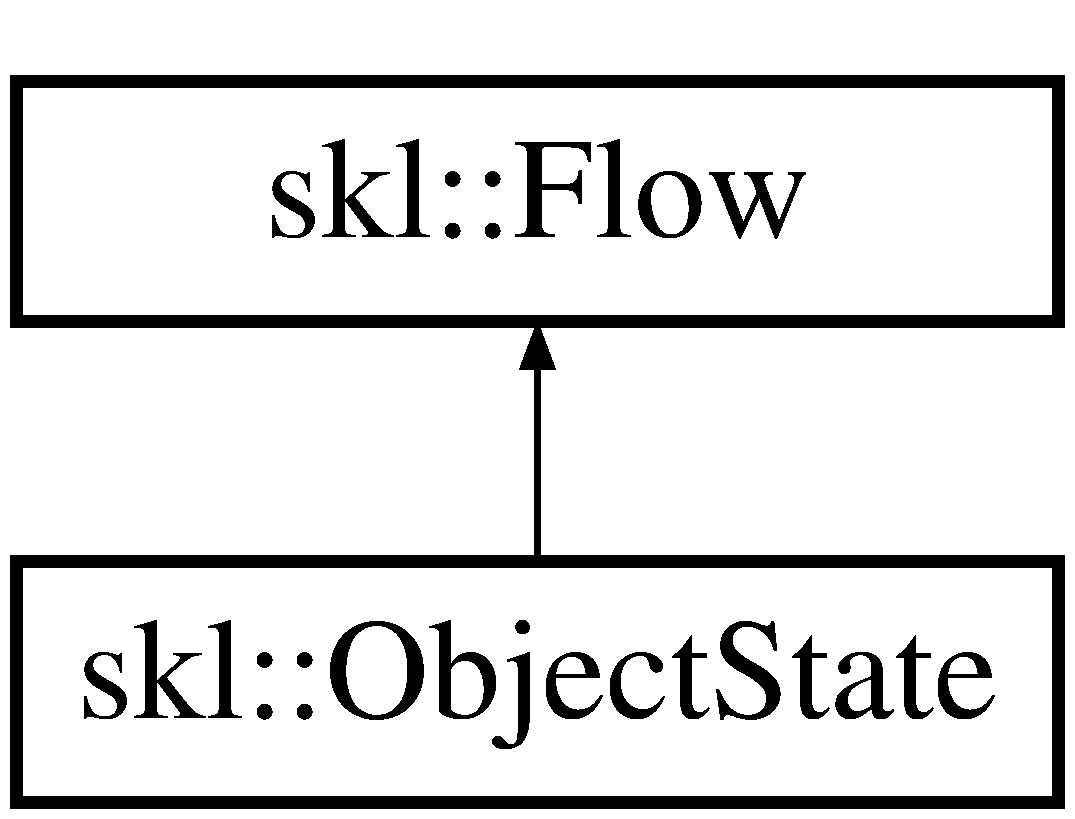
\includegraphics[height=2.000000cm]{classskl_1_1_flow}
\end{center}
\end{figure}
\subsection*{Public Types}
\begin{DoxyCompactItemize}
\item 
\hypertarget{classskl_1_1_flow_a13fd439f2bea3c780a8db9869513f05c}{}\label{classskl_1_1_flow_a13fd439f2bea3c780a8db9869513f05c} 
enum {\bfseries Direction} \{ {\bfseries X} =0, 
{\bfseries Y} =1
 \}
\end{DoxyCompactItemize}
\subsection*{Public Member Functions}
\begin{DoxyCompactItemize}
\item 
\hypertarget{classskl_1_1_flow_ac9975e144e606242748197798e87dd32}{}\label{classskl_1_1_flow_ac9975e144e606242748197798e87dd32} 
\hyperlink{classskl_1_1_flow_ac9975e144e606242748197798e87dd32}{Flow} ()
\begin{DoxyCompactList}\small\item\em デフォルトコンストラクタ \end{DoxyCompactList}\item 
\hypertarget{classskl_1_1_flow_a5a65e36c874c5cd5283ac32a33eb0a8b}{}\label{classskl_1_1_flow_a5a65e36c874c5cd5283ac32a33eb0a8b} 
\hyperlink{classskl_1_1_flow_a5a65e36c874c5cd5283ac32a33eb0a8b}{Flow} (const \hyperlink{classskl_1_1_flow}{Flow} \&other)
\begin{DoxyCompactList}\small\item\em Shallow Copyするコンストラクタ \end{DoxyCompactList}\item 
\hypertarget{classskl_1_1_flow_ae3ff785a69417be037a89377215e82a2}{}\label{classskl_1_1_flow_ae3ff785a69417be037a89377215e82a2} 
\hyperlink{classskl_1_1_flow_ae3ff785a69417be037a89377215e82a2}{Flow} (const cv\+::\+Mat \&u, const cv\+::\+Mat \&v)
\begin{DoxyCompactList}\small\item\em Constractor which sets u and v. \end{DoxyCompactList}\item 
\hypertarget{classskl_1_1_flow_a112fcdcc7ef094f98efe49d2f58e3024}{}\label{classskl_1_1_flow_a112fcdcc7ef094f98efe49d2f58e3024} 
\hyperlink{classskl_1_1_flow}{Flow} {\bfseries clone} () const
\item 
\hypertarget{classskl_1_1_flow_a5991efa6e8cf88c4ef2125cc727db333}{}\label{classskl_1_1_flow_a5991efa6e8cf88c4ef2125cc727db333} 
virtual \hyperlink{classskl_1_1_flow_a5991efa6e8cf88c4ef2125cc727db333}{$\sim$\+Flow} ()
\begin{DoxyCompactList}\small\item\em デストラクタ \end{DoxyCompactList}\item 
\hypertarget{classskl_1_1_flow_a0b978694e74a5b9fbd9cda8c30c81748}{}\label{classskl_1_1_flow_a0b978694e74a5b9fbd9cda8c30c81748} 
\hyperlink{classskl_1_1_flow}{Flow} \& {\bfseries operator=} (const \hyperlink{classskl_1_1_flow}{Flow} \&other)
\item 
void \hyperlink{classskl_1_1_flow_af771e593b403a1b807ec5564409188f1}{distance} (cv\+::\+Mat \&r)
\item 
\hypertarget{classskl_1_1_flow_aad7005f577155b3486db299c36926b65}{}\label{classskl_1_1_flow_aad7005f577155b3486db299c36926b65} 
cv\+::\+Mat {\bfseries distance} ()
\item 
\hypertarget{classskl_1_1_flow_ab52e31d8d97e1ea2e7d6258a40636055}{}\label{classskl_1_1_flow_ab52e31d8d97e1ea2e7d6258a40636055} 
const cv\+::\+Mat \& {\bfseries operator\mbox{[}$\,$\mbox{]}} (Direction d) const
\item 
\hypertarget{classskl_1_1_flow_ad25fe4621fb0a59cf11f897369cf6ad8}{}\label{classskl_1_1_flow_ad25fe4621fb0a59cf11f897369cf6ad8} 
cv\+::\+Mat \& {\bfseries operator\mbox{[}$\,$\mbox{]}} (Direction d)
\item 
\hypertarget{classskl_1_1_flow_a28aebd0d1764c11106df8b71fc3651ee}{}\label{classskl_1_1_flow_a28aebd0d1764c11106df8b71fc3651ee} 
void {\bfseries angle} (cv\+::\+Mat \&rad, float offset\+\_\+rad=0, float origin\+\_\+return\+\_\+value=0)
\item 
\hypertarget{classskl_1_1_flow_a05c0dd2eb0f250678497977ce8f2c4cd}{}\label{classskl_1_1_flow_a05c0dd2eb0f250678497977ce8f2c4cd} 
cv\+::\+Mat {\bfseries angle} (float offset\+\_\+rad=0, float origin\+\_\+return\+\_\+value=0)
\item 
\hypertarget{classskl_1_1_flow_ae80c303a98e877b5573bbeffcd9d96a4}{}\label{classskl_1_1_flow_ae80c303a98e877b5573bbeffcd9d96a4} 
cv\+::\+Mat {\bfseries visualize} (cv\+::\+Mat \&base, int interval=8, const cv\+::\+Scalar \&arrow\+\_\+color=C\+V\+\_\+\+R\+GB(255, 0, 0))
\item 
\hypertarget{classskl_1_1_flow_a931d778cd2124acacf264777cae38eee}{}\label{classskl_1_1_flow_a931d778cd2124acacf264777cae38eee} 
bool {\bfseries read} (const std\+::string \&filename)
\item 
\hypertarget{classskl_1_1_flow_a3696523a55d599b88d4971eb3d023fea}{}\label{classskl_1_1_flow_a3696523a55d599b88d4971eb3d023fea} 
bool {\bfseries write} (const std\+::string \&filename) const
\end{DoxyCompactItemize}
\subsection*{Public Attributes}
\begin{DoxyCompactItemize}
\item 
\hypertarget{classskl_1_1_flow_a2aa676dc599de74aa6776946d697d0e0}{}\label{classskl_1_1_flow_a2aa676dc599de74aa6776946d697d0e0} 
cv\+::\+Mat {\bfseries u}
\item 
\hypertarget{classskl_1_1_flow_a1ecd332e688a2766d7946bce1707c4a0}{}\label{classskl_1_1_flow_a1ecd332e688a2766d7946bce1707c4a0} 
cv\+::\+Mat {\bfseries v}
\end{DoxyCompactItemize}
\subsection*{Protected Member Functions}
\begin{DoxyCompactItemize}
\item 
\hypertarget{classskl_1_1_flow_a98eb935c6ac591992afcfa718ab44964}{}\label{classskl_1_1_flow_a98eb935c6ac591992afcfa718ab44964} 
bool \hyperlink{classskl_1_1_flow_a98eb935c6ac591992afcfa718ab44964}{is\+Valid} () const
\begin{DoxyCompactList}\small\item\em check size and type of u and v. \end{DoxyCompactList}\end{DoxyCompactItemize}


\subsection{Detailed Description}
Class for optical flow. 

\subsection{Member Function Documentation}
\hypertarget{classskl_1_1_flow_af771e593b403a1b807ec5564409188f1}{}\label{classskl_1_1_flow_af771e593b403a1b807ec5564409188f1} 
\index{skl\+::\+Flow@{skl\+::\+Flow}!distance@{distance}}
\index{distance@{distance}!skl\+::\+Flow@{skl\+::\+Flow}}
\subsubsection{\texorpdfstring{distance()}{distance()}}
{\footnotesize\ttfamily void Flow\+::distance (\begin{DoxyParamCaption}\item[{cv\+::\+Mat \&}]{r }\end{DoxyParamCaption})}

convert \{u,v\} to moved distance sqrt(u$^\wedge$2+v$^\wedge$2) 

The documentation for this class was generated from the following files\+:\begin{DoxyCompactItemize}
\item 
Open\+C\+V/include/\hyperlink{_flow_8h}{Flow.\+h}\item 
Open\+C\+V/src/\hyperlink{_flow_8cpp}{Flow.\+cpp}\end{DoxyCompactItemize}

\hypertarget{classskl_1_1_graphcut}{}\section{skl\+:\+:Graphcut Class Reference}
\label{classskl_1_1_graphcut}\index{skl\+::\+Graphcut@{skl\+::\+Graphcut}}


Wrapper Class of graphcut by Vladimir Komogorov.  




{\ttfamily \#include $<$Graphcut.\+h$>$}

\subsection*{Public Member Functions}
\begin{DoxyCompactItemize}
\item 
\hypertarget{classskl_1_1_graphcut_a1a784d4591dfd733eee7f172f56ae23b}{}\label{classskl_1_1_graphcut_a1a784d4591dfd733eee7f172f56ae23b} 
\hyperlink{classskl_1_1_graphcut_a1a784d4591dfd733eee7f172f56ae23b}{Graphcut} ()
\begin{DoxyCompactList}\small\item\em デフォルトコンストラクタ \end{DoxyCompactList}\item 
\hypertarget{classskl_1_1_graphcut_aadfc7d0fea926aac3e88be1930239adb}{}\label{classskl_1_1_graphcut_aadfc7d0fea926aac3e88be1930239adb} 
virtual \hyperlink{classskl_1_1_graphcut_aadfc7d0fea926aac3e88be1930239adb}{$\sim$\+Graphcut} ()
\begin{DoxyCompactList}\small\item\em デストラクタ \end{DoxyCompactList}\item 
\hypertarget{classskl_1_1_graphcut_add5ffe56f886d143450050e2fe1a6ae8}{}\label{classskl_1_1_graphcut_add5ffe56f886d143450050e2fe1a6ae8} 
int {\bfseries compute} (const cv\+::\+Mat \&terminals, const cv\+::\+Mat \&left\+Transp, const cv\+::\+Mat \&right\+Transp, const cv\+::\+Mat \&top, const cv\+::\+Mat \&bottom, cv\+::\+Mat \&dest)
\end{DoxyCompactItemize}
\subsection*{Protected Attributes}
\begin{DoxyCompactItemize}
\item 
\hypertarget{classskl_1_1_graphcut_ae41c06b9e782bd69d2633760c32cfc53}{}\label{classskl_1_1_graphcut_ae41c06b9e782bd69d2633760c32cfc53} 
Graph$<$ int, int, int $>$ $\ast$ {\bfseries graph}
\item 
\hypertarget{classskl_1_1_graphcut_a3dfcbf111a5d66f386d4ee6b5daccc77}{}\label{classskl_1_1_graphcut_a3dfcbf111a5d66f386d4ee6b5daccc77} 
std\+::vector$<$ std\+::vector$<$ Graph$<$ int, int, int $>$\+::node\+\_\+id $>$ $>$ {\bfseries nodes}
\item 
\hypertarget{classskl_1_1_graphcut_acc37076a1fb4ed536fd0ba089f019b20}{}\label{classskl_1_1_graphcut_acc37076a1fb4ed536fd0ba089f019b20} 
cv\+::\+Size {\bfseries graph\+\_\+size}
\item 
\hypertarget{classskl_1_1_graphcut_a2438ccbecf54676accbda142f0c641ea}{}\label{classskl_1_1_graphcut_a2438ccbecf54676accbda142f0c641ea} 
size\+\_\+t {\bfseries graph\+\_\+node\+\_\+num}
\end{DoxyCompactItemize}


\subsection{Detailed Description}
Wrapper Class of graphcut by Vladimir Komogorov. 

The documentation for this class was generated from the following files\+:\begin{DoxyCompactItemize}
\item 
Open\+C\+V/include/\hyperlink{_graphcut_8h}{Graphcut.\+h}\item 
Open\+C\+V/src/\hyperlink{_graphcut_8cpp}{Graphcut.\+cpp}\end{DoxyCompactItemize}

\hypertarget{classskl_1_1_h_t_t_p_client}{}\section{skl\+:\+:H\+T\+T\+P\+Client Class Reference}
\label{classskl_1_1_h_t_t_p_client}\index{skl\+::\+H\+T\+T\+P\+Client@{skl\+::\+H\+T\+T\+P\+Client}}


\hyperlink{classskl_1_1_h_t_t_p_client}{H\+T\+T\+P\+Client} get/post requestを送るクラス(redirectには対応していない簡単なもの)  




{\ttfamily \#include $<$H\+T\+T\+P\+Client.\+h$>$}

Inheritance diagram for skl\+:\+:H\+T\+T\+P\+Client\+:\begin{figure}[H]
\begin{center}
\leavevmode
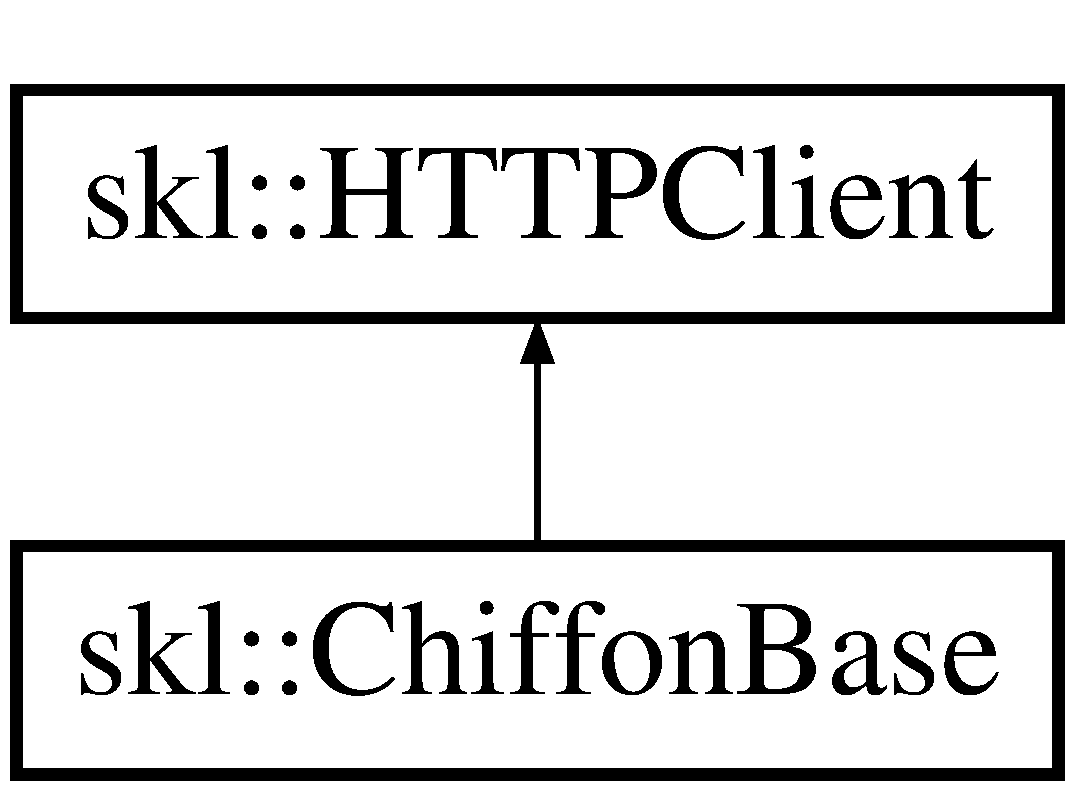
\includegraphics[height=2.000000cm]{classskl_1_1_h_t_t_p_client}
\end{center}
\end{figure}
\subsection*{Classes}
\begin{DoxyCompactItemize}
\item 
class \hyperlink{classskl_1_1_h_t_t_p_client_1_1tcp__client}{tcp\+\_\+client}
\end{DoxyCompactItemize}
\subsection*{Public Member Functions}
\begin{DoxyCompactItemize}
\item 
\hypertarget{classskl_1_1_h_t_t_p_client_aa51f43aef6208916f62669de3fed1de0}{}\label{classskl_1_1_h_t_t_p_client_aa51f43aef6208916f62669de3fed1de0} 
{\bfseries H\+T\+T\+P\+Client} (const std\+::string \&host, int port=80)
\item 
\hypertarget{classskl_1_1_h_t_t_p_client_adea8587355607c4fdde6e6c85d445fc9}{}\label{classskl_1_1_h_t_t_p_client_adea8587355607c4fdde6e6c85d445fc9} 
bool {\bfseries get} (const std\+::string \&path, const std\+::string \&query=\char`\"{}\char`\"{})
\item 
\hypertarget{classskl_1_1_h_t_t_p_client_af319583a773165209adc257bd7a3cef9}{}\label{classskl_1_1_h_t_t_p_client_af319583a773165209adc257bd7a3cef9} 
bool {\bfseries post} (const std\+::string \&path, const std\+::string \&query)
\item 
\hypertarget{classskl_1_1_h_t_t_p_client_a3727336ba1c411c3d10949f31a987c27}{}\label{classskl_1_1_h_t_t_p_client_a3727336ba1c411c3d10949f31a987c27} 
unsigned int {\bfseries status\+\_\+code} () const
\item 
\hypertarget{classskl_1_1_h_t_t_p_client_a8ce4445d43ff331ed51cce35d66a95c6}{}\label{classskl_1_1_h_t_t_p_client_a8ce4445d43ff331ed51cce35d66a95c6} 
const std\+::string \& {\bfseries read} () const
\item 
\hypertarget{classskl_1_1_h_t_t_p_client_a1679219321139d2306e101d251de73c4}{}\label{classskl_1_1_h_t_t_p_client_a1679219321139d2306e101d251de73c4} 
std\+::map$<$ std\+::string, std\+::string $>$ {\bfseries header} () const
\end{DoxyCompactItemize}
\subsection*{Protected Types}
\begin{DoxyCompactItemize}
\item 
\hypertarget{classskl_1_1_h_t_t_p_client_a7911f896b7d883ac33814684deb03dfa}{}\label{classskl_1_1_h_t_t_p_client_a7911f896b7d883ac33814684deb03dfa} 
typedef boost\+::shared\+\_\+ptr$<$ \hyperlink{classskl_1_1_h_t_t_p_client_1_1tcp__client}{tcp\+\_\+client} $>$ {\bfseries tcp\+\_\+client\+\_\+ptr}
\end{DoxyCompactItemize}
\subsection*{Protected Member Functions}
\begin{DoxyCompactItemize}
\item 
\hypertarget{classskl_1_1_h_t_t_p_client_a74c9a575106b741ad6cfd95f3932de18}{}\label{classskl_1_1_h_t_t_p_client_a74c9a575106b741ad6cfd95f3932de18} 
void {\bfseries make\+Request} (boost\+::asio\+::streambuf \&buf, const std\+::string \&path, const std\+::string \&query=\char`\"{}\char`\"{}) const
\item 
\hypertarget{classskl_1_1_h_t_t_p_client_a00b88c67fa4c2c817b32150541901f12}{}\label{classskl_1_1_h_t_t_p_client_a00b88c67fa4c2c817b32150541901f12} 
bool {\bfseries Url\+Encode} (std\+::string \&str) const
\end{DoxyCompactItemize}
\subsection*{Protected Attributes}
\begin{DoxyCompactItemize}
\item 
\hypertarget{classskl_1_1_h_t_t_p_client_a0e44c47f71676bcfc6ff79df3eaa60fb}{}\label{classskl_1_1_h_t_t_p_client_a0e44c47f71676bcfc6ff79df3eaa60fb} 
std\+::string {\bfseries host\+\_\+}
\item 
\hypertarget{classskl_1_1_h_t_t_p_client_a8676f73a1afa20928a4c5b9b4a781ddf}{}\label{classskl_1_1_h_t_t_p_client_a8676f73a1afa20928a4c5b9b4a781ddf} 
int {\bfseries port\+\_\+}
\item 
\hypertarget{classskl_1_1_h_t_t_p_client_a05b976dc2f1ca592c87a7a78d5b0d909}{}\label{classskl_1_1_h_t_t_p_client_a05b976dc2f1ca592c87a7a78d5b0d909} 
boost\+::asio\+::io\+\_\+service {\bfseries io\+\_\+service\+\_\+}
\item 
\hypertarget{classskl_1_1_h_t_t_p_client_ae756b586bde61e8fb606bda4d281975c}{}\label{classskl_1_1_h_t_t_p_client_ae756b586bde61e8fb606bda4d281975c} 
tcp\+\_\+client\+\_\+ptr {\bfseries tcp\+\_\+base\+\_\+}
\end{DoxyCompactItemize}


\subsection{Detailed Description}
\hyperlink{classskl_1_1_h_t_t_p_client}{H\+T\+T\+P\+Client} get/post requestを送るクラス(redirectには対応していない簡単なもの) 

The documentation for this class was generated from the following file\+:\begin{DoxyCompactItemize}
\item 
Core/include/\hyperlink{_h_t_t_p_client_8h}{H\+T\+T\+P\+Client.\+h}\end{DoxyCompactItemize}

\hypertarget{classskl_1_1_human_detector_workspace_end}{}\section{skl\+:\+:Human\+Detector\+Workspace\+End Class Reference}
\label{classskl_1_1_human_detector_workspace_end}\index{skl\+::\+Human\+Detector\+Workspace\+End@{skl\+::\+Human\+Detector\+Workspace\+End}}
Inheritance diagram for skl\+:\+:Human\+Detector\+Workspace\+End\+:\begin{figure}[H]
\begin{center}
\leavevmode
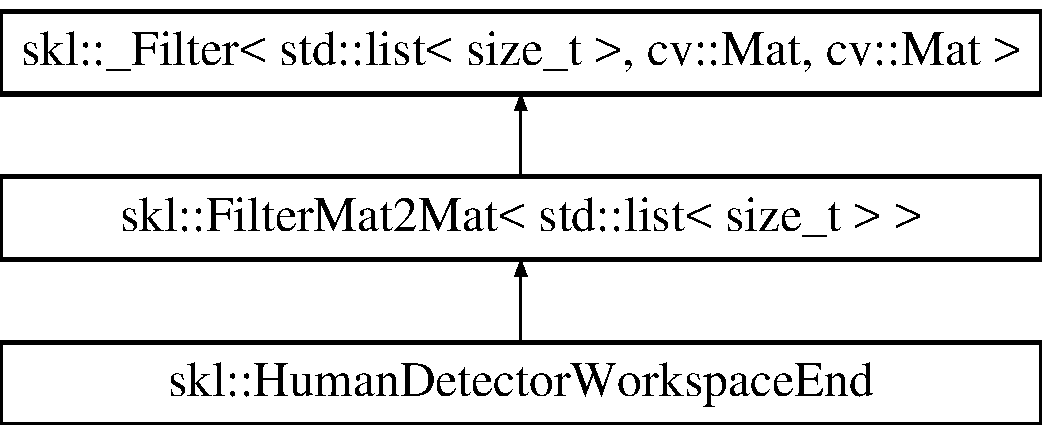
\includegraphics[height=3.000000cm]{classskl_1_1_human_detector_workspace_end}
\end{center}
\end{figure}
\subsection*{Public Member Functions}
\begin{DoxyCompactItemize}
\item 
\hypertarget{classskl_1_1_human_detector_workspace_end_a81308660a9fba4b4e85ce182a7e319b4}{}\label{classskl_1_1_human_detector_workspace_end_a81308660a9fba4b4e85ce182a7e319b4} 
{\bfseries Human\+Detector\+Workspace\+End} (const cv\+::\+Mat \&workspace\+\_\+end)
\item 
\hypertarget{classskl_1_1_human_detector_workspace_end_af2ce04d4506038af6c46ece4e527a2d5}{}\label{classskl_1_1_human_detector_workspace_end_af2ce04d4506038af6c46ece4e527a2d5} 
void {\bfseries set\+Workspace\+End} (const cv\+::\+Mat \&workspace\+\_\+end)
\item 
\hypertarget{classskl_1_1_human_detector_workspace_end_a8ef7d03cf0962270f4d87e5771e3cd9c}{}\label{classskl_1_1_human_detector_workspace_end_a8ef7d03cf0962270f4d87e5771e3cd9c} 
std\+::list$<$ size\+\_\+t $>$ {\bfseries compute} (const cv\+::\+Mat \&src, const cv\+::\+Mat \&mask, cv\+::\+Mat \&human\+\_\+region)
\end{DoxyCompactItemize}
\subsection*{Protected Attributes}
\begin{DoxyCompactItemize}
\item 
\hypertarget{classskl_1_1_human_detector_workspace_end_ae55e80388c04d082c8b4727d0bb825bf}{}\label{classskl_1_1_human_detector_workspace_end_ae55e80388c04d082c8b4727d0bb825bf} 
cv\+::\+Mat {\bfseries workspace\+\_\+end}
\end{DoxyCompactItemize}


The documentation for this class was generated from the following files\+:\begin{DoxyCompactItemize}
\item 
Open\+C\+V/include/Human\+Detector\+Workspace\+End.\+h\item 
Open\+C\+V/src/Human\+Detector\+Workspace\+End.\+cpp\end{DoxyCompactItemize}

\hypertarget{classskl_1_1_key_input}{}\section{skl\+:\+:Key\+Input Class Reference}
\label{classskl_1_1_key_input}\index{skl\+::\+Key\+Input@{skl\+::\+Key\+Input}}
\subsection*{Public Types}
\begin{DoxyCompactItemize}
\item 
\hypertarget{classskl_1_1_key_input_a3041907e37053b075d2204f07e790cbb}{}\label{classskl_1_1_key_input_a3041907e37053b075d2204f07e790cbb} 
enum \{ \newline
{\bfseries S\+H\+I\+FT} = 0x10000, 
{\bfseries C\+T\+RL} = 0x40000, 
{\bfseries N\+U\+M\+L\+O\+CK} = 0x100000, 
{\bfseries C\+A\+P\+S\+L\+O\+CK} = 0x20000, 
\newline
{\bfseries A\+LT} = 0x80000, 
{\bfseries L\+E\+F\+T\+\_\+\+A\+R\+R\+OW} = 65361, 
{\bfseries U\+P\+\_\+\+A\+R\+R\+OW} = 65362, 
{\bfseries R\+I\+G\+H\+T\+\_\+\+A\+R\+R\+OW} = 65363, 
\newline
{\bfseries D\+O\+W\+N\+\_\+\+A\+R\+R\+OW} = 65364
 \}
\end{DoxyCompactItemize}
\subsection*{Public Member Functions}
\begin{DoxyCompactItemize}
\item 
\hypertarget{classskl_1_1_key_input_a433d183979067662820d7b929e249b95}{}\label{classskl_1_1_key_input_a433d183979067662820d7b929e249b95} 
char {\bfseries set} (int keystroke)
\item 
\hypertarget{classskl_1_1_key_input_a9590de3ef1f3b34e1371090fc02d3b80}{}\label{classskl_1_1_key_input_a9590de3ef1f3b34e1371090fc02d3b80} 
char {\bfseries get\+Char} ()
\item 
\hypertarget{classskl_1_1_key_input_a8e3f6b5a26823d68b42bd3373376d712}{}\label{classskl_1_1_key_input_a8e3f6b5a26823d68b42bd3373376d712} 
bool {\bfseries is\+Valid} ()
\item 
\hypertarget{classskl_1_1_key_input_a5d705978e5e08298d21ccc5efe574f03}{}\label{classskl_1_1_key_input_a5d705978e5e08298d21ccc5efe574f03} 
int {\bfseries code} () const
\item 
\hypertarget{classskl_1_1_key_input_adcad47367d0a140fa7d56ada00fbce9a}{}\label{classskl_1_1_key_input_adcad47367d0a140fa7d56ada00fbce9a} 
bool {\bfseries shift} () const
\item 
\hypertarget{classskl_1_1_key_input_ad62de27cadf145a1a3321c0dbcfa2f81}{}\label{classskl_1_1_key_input_ad62de27cadf145a1a3321c0dbcfa2f81} 
bool {\bfseries ctrl} () const
\item 
\hypertarget{classskl_1_1_key_input_a9561162d5ffd33754b806e3d2bf9b8b2}{}\label{classskl_1_1_key_input_a9561162d5ffd33754b806e3d2bf9b8b2} 
bool {\bfseries numlock} () const
\item 
\hypertarget{classskl_1_1_key_input_adb125489e60f7eaa0d32c048a0544841}{}\label{classskl_1_1_key_input_adb125489e60f7eaa0d32c048a0544841} 
bool {\bfseries capslock} () const
\item 
\hypertarget{classskl_1_1_key_input_aa8928da3627ae3556198e7e2e3a5af10}{}\label{classskl_1_1_key_input_aa8928da3627ae3556198e7e2e3a5af10} 
bool {\bfseries alt} () const
\end{DoxyCompactItemize}
\subsection*{Protected Attributes}
\begin{DoxyCompactItemize}
\item 
\hypertarget{classskl_1_1_key_input_ab7c445dee3b0c2de8c266dd7a2eb2b00}{}\label{classskl_1_1_key_input_ab7c445dee3b0c2de8c266dd7a2eb2b00} 
int {\bfseries \+\_\+code}
\item 
\hypertarget{classskl_1_1_key_input_a537fbedb395a46169c3c99af808691e1}{}\label{classskl_1_1_key_input_a537fbedb395a46169c3c99af808691e1} 
bool {\bfseries \+\_\+shift}
\item 
\hypertarget{classskl_1_1_key_input_a5efcbdadc726872cae91386163c84bdf}{}\label{classskl_1_1_key_input_a5efcbdadc726872cae91386163c84bdf} 
bool {\bfseries \+\_\+ctrl}
\item 
\hypertarget{classskl_1_1_key_input_a9c3c98ec877767c743853c7367e4747c}{}\label{classskl_1_1_key_input_a9c3c98ec877767c743853c7367e4747c} 
bool {\bfseries \+\_\+numlock}
\item 
\hypertarget{classskl_1_1_key_input_a17d3c07d17ecd1195078790cf712f4cb}{}\label{classskl_1_1_key_input_a17d3c07d17ecd1195078790cf712f4cb} 
bool {\bfseries \+\_\+capslock}
\item 
\hypertarget{classskl_1_1_key_input_a0bb09cf95828ac5fb0df5a62e7559423}{}\label{classskl_1_1_key_input_a0bb09cf95828ac5fb0df5a62e7559423} 
bool {\bfseries \+\_\+alt}
\item 
\hypertarget{classskl_1_1_key_input_a4205ff6d7423d192ab8bc97bd0874d99}{}\label{classskl_1_1_key_input_a4205ff6d7423d192ab8bc97bd0874d99} 
bool {\bfseries is\+\_\+valid}
\end{DoxyCompactItemize}


The documentation for this class was generated from the following files\+:\begin{DoxyCompactItemize}
\item 
Core/include/\hyperlink{_key_input_8h}{Key\+Input.\+h}\item 
Core/src/\hyperlink{_key_input_8cpp}{Key\+Input.\+cpp}\end{DoxyCompactItemize}

\hypertarget{class_labeling}{}\section{Labeling$<$ SrcT, DstT $>$ Class Template Reference}
\label{class_labeling}\index{Labeling$<$ Src\+T, Dst\+T $>$@{Labeling$<$ Src\+T, Dst\+T $>$}}
\subsection*{Classes}
\begin{DoxyCompactItemize}
\item 
class \hyperlink{class_labeling_1_1_raster_segment}{Raster\+Segment}
\begin{DoxyCompactList}\small\item\em \hyperlink{class_labeling_1_1_raster_segment}{Raster\+Segment}. \end{DoxyCompactList}\item 
class \hyperlink{class_labeling_1_1_region_info}{Region\+Info}
\end{DoxyCompactItemize}
\subsection*{Public Types}
\begin{DoxyCompactItemize}
\item 
\hypertarget{class_labeling_aed2219f3d8b3a803d96da6750834fe16}{}\label{class_labeling_aed2219f3d8b3a803d96da6750834fe16} 
typedef std\+::list$<$ \hyperlink{class_labeling_1_1_raster_segment}{Raster\+Segment} $\ast$ $>$ {\bfseries R\+S\+P\+List}
\item 
\hypertarget{class_labeling_a8a57d7361dcb88b2aba008ac3369f8df}{}\label{class_labeling_a8a57d7361dcb88b2aba008ac3369f8df} 
typedef std\+::list$<$ \hyperlink{class_labeling_1_1_raster_segment}{Raster\+Segment} $\ast$ $>$\+::iterator {\bfseries R\+S\+P\+Iterator}
\item 
\hypertarget{class_labeling_ad6742d43c058dda1a526f114a41955d6}{}\label{class_labeling_ad6742d43c058dda1a526f114a41955d6} 
typedef std\+::queue$<$ \hyperlink{class_labeling_1_1_raster_segment}{Raster\+Segment} $\ast$ $>$ {\bfseries R\+S\+P\+Queue}
\item 
\hypertarget{class_labeling_a268813d6a00e26c7b524122bd2d88596}{}\label{class_labeling_a268813d6a00e26c7b524122bd2d88596} 
typedef std\+::list$<$ \hyperlink{class_labeling_1_1_region_info}{Region\+Info} $\ast$ $>$ {\bfseries R\+I\+P\+List}
\item 
\hypertarget{class_labeling_a9264d38d8c52860116e8a751bb0a75eb}{}\label{class_labeling_a9264d38d8c52860116e8a751bb0a75eb} 
typedef std\+::list$<$ \hyperlink{class_labeling_1_1_region_info}{Region\+Info} $\ast$ $>$\+::iterator {\bfseries R\+I\+P\+Iterator}
\item 
\hypertarget{class_labeling_aecf75ed5a0fa2ee88a1b24e09af35f8c}{}\label{class_labeling_aecf75ed5a0fa2ee88a1b24e09af35f8c} 
typedef std\+::vector$<$ \hyperlink{class_labeling_1_1_region_info}{Region\+Info} $\ast$ $>$ {\bfseries R\+I\+P\+Vector}
\end{DoxyCompactItemize}
\subsection*{Public Member Functions}
\begin{DoxyCompactItemize}
\item 
\hypertarget{class_labeling_a7ef9dffc4fdda47cab7bd87d16419bcc}{}\label{class_labeling_a7ef9dffc4fdda47cab7bd87d16419bcc} 
int {\bfseries Get\+Num\+Of\+Regions} (void) const
\item 
\hypertarget{class_labeling_ac459520ccd9b51c42c9e19aa08dd49d2}{}\label{class_labeling_ac459520ccd9b51c42c9e19aa08dd49d2} 
int {\bfseries Get\+Num\+Of\+Result\+Regions} (void) const
\item 
\hypertarget{class_labeling_a61c657da16920ffd8570c9ffa6fe7c1a}{}\label{class_labeling_a61c657da16920ffd8570c9ffa6fe7c1a} 
\hyperlink{class_labeling_1_1_region_info}{Region\+Info} $\ast$ {\bfseries Get\+Result\+Region\+Info} (const int num) const
\item 
int \hyperlink{class_labeling_a639673f1a391609c6a78f46b0575774a}{Exec} (SrcT $\ast$target, DstT $\ast$result, int target\+\_\+width, int target\+\_\+height, const bool is\+\_\+sort\+\_\+region, const int region\+\_\+size\+\_\+min)
\begin{DoxyCompactList}\small\item\em ラベリング処理を実行。処理後、\+Dst\+Tには\mbox{[}0,\#region\mbox{]}までのいずれかの値が格納される。 \end{DoxyCompactList}\end{DoxyCompactItemize}


\subsection{Member Function Documentation}
\hypertarget{class_labeling_a639673f1a391609c6a78f46b0575774a}{}\label{class_labeling_a639673f1a391609c6a78f46b0575774a} 
\index{Labeling@{Labeling}!Exec@{Exec}}
\index{Exec@{Exec}!Labeling@{Labeling}}
\subsubsection{\texorpdfstring{Exec()}{Exec()}}
{\footnotesize\ttfamily template$<$class SrcT, class DstT$>$ \\
int \hyperlink{class_labeling}{Labeling}$<$ SrcT, DstT $>$\+::Exec (\begin{DoxyParamCaption}\item[{SrcT $\ast$}]{target,  }\item[{DstT $\ast$}]{result,  }\item[{int}]{target\+\_\+width,  }\item[{int}]{target\+\_\+height,  }\item[{const bool}]{is\+\_\+sort\+\_\+region,  }\item[{const int}]{region\+\_\+size\+\_\+min }\end{DoxyParamCaption})\hspace{0.3cm}{\ttfamily [inline]}}



ラベリング処理を実行。処理後、\+Dst\+Tには\mbox{[}0,\#region\mbox{]}までのいずれかの値が格納される。 


\begin{DoxyParams}[1]{Parameters}
\mbox{\tt out}  & {\em DstT} & DstT\mbox{[}x,y\mbox{]}=0ならば背景領域、\+DstT\mbox{[}x,y\mbox{]}=kならばk番目の領域を表す。 \\
\hline
\end{DoxyParams}


The documentation for this class was generated from the following file\+:\begin{DoxyCompactItemize}
\item 
Open\+C\+V/include/\hyperlink{_labeling_8h}{Labeling.\+h}\end{DoxyCompactItemize}

\hypertarget{class_main_loop_runner}{}\section{Main\+Loop\+Runner Class Reference}
\label{class_main_loop_runner}\index{Main\+Loop\+Runner@{Main\+Loop\+Runner}}
Inheritance diagram for Main\+Loop\+Runner\+:\begin{figure}[H]
\begin{center}
\leavevmode
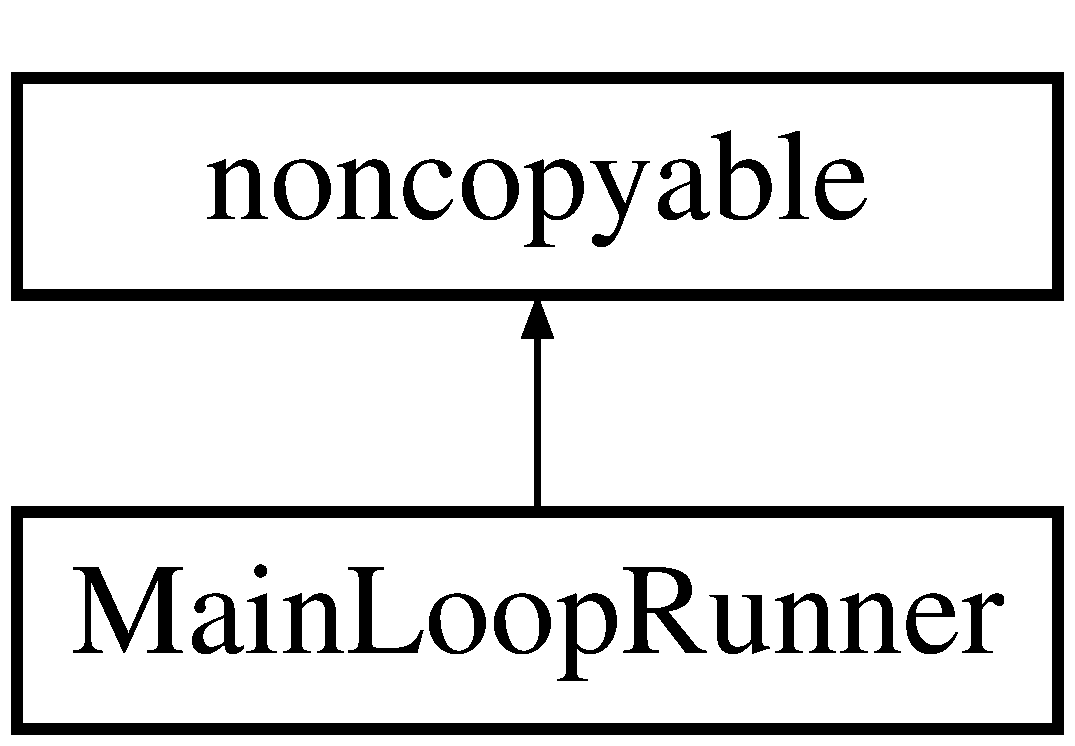
\includegraphics[height=2.000000cm]{class_main_loop_runner}
\end{center}
\end{figure}
\subsection*{Public Member Functions}
\begin{DoxyCompactItemize}
\item 
\hypertarget{class_main_loop_runner_a90cb92e187a7e697bba8e6a7c0c0896e}{}\label{class_main_loop_runner_a90cb92e187a7e697bba8e6a7c0c0896e} 
tetio\+::\+Main\+Loop \& {\bfseries get\+Main\+Loop} ()
\item 
\hypertarget{class_main_loop_runner_a1c132147e055edb44a23f8d2bc384880}{}\label{class_main_loop_runner_a1c132147e055edb44a23f8d2bc384880} 
void {\bfseries start} ()
\item 
\hypertarget{class_main_loop_runner_ac566cf89b46777a383c89888167972bc}{}\label{class_main_loop_runner_ac566cf89b46777a383c89888167972bc} 
void {\bfseries stop} ()
\end{DoxyCompactItemize}


The documentation for this class was generated from the following file\+:\begin{DoxyCompactItemize}
\item 
Core/include/Main\+Loop\+Runner.\+h\end{DoxyCompactItemize}

\hypertarget{classskl_1_1_mat_reader}{}\section{skl\+:\+:Mat\+Reader$<$ Elem\+Type, C\+V\+\_\+\+T\+Y\+PE $>$ Class Template Reference}
\label{classskl_1_1_mat_reader}\index{skl\+::\+Mat\+Reader$<$ Elem\+Type, C\+V\+\_\+\+T\+Y\+P\+E $>$@{skl\+::\+Mat\+Reader$<$ Elem\+Type, C\+V\+\_\+\+T\+Y\+P\+E $>$}}


read cv\+::\+Mat data from file, which was output by operator$<$$<$(). (only for 1 channel matrix)  




{\ttfamily \#include $<$Mat\+Reader.\+h$>$}

\subsection*{Public Member Functions}
\begin{DoxyCompactItemize}
\item 
\hypertarget{classskl_1_1_mat_reader_aad30f39108fd650864d1924c2d85fe65}{}\label{classskl_1_1_mat_reader_aad30f39108fd650864d1924c2d85fe65} 
\hyperlink{classskl_1_1_mat_reader_aad30f39108fd650864d1924c2d85fe65}{Mat\+Reader} ()
\begin{DoxyCompactList}\small\item\em デフォルトコンストラクタ \end{DoxyCompactList}\item 
\hypertarget{classskl_1_1_mat_reader_a9e6ad16602f3b5b2bc9118c4eb28d211}{}\label{classskl_1_1_mat_reader_a9e6ad16602f3b5b2bc9118c4eb28d211} 
virtual \hyperlink{classskl_1_1_mat_reader_a9e6ad16602f3b5b2bc9118c4eb28d211}{$\sim$\+Mat\+Reader} ()
\begin{DoxyCompactList}\small\item\em デストラクタ \end{DoxyCompactList}\end{DoxyCompactItemize}
\subsection*{Static Public Member Functions}
\begin{DoxyCompactItemize}
\item 
\hypertarget{classskl_1_1_mat_reader_a55b939ebe0e753199b1a186aaff9006f}{}\label{classskl_1_1_mat_reader_a55b939ebe0e753199b1a186aaff9006f} 
static bool {\bfseries read} (const std\+::string \&filename, cv\+::\+Mat \&mat, const std\+::string \&deliminator=\char`\"{},\char`\"{})
\item 
\hypertarget{classskl_1_1_mat_reader_a23765ba40ad293cc49ab2e82904ed6b1}{}\label{classskl_1_1_mat_reader_a23765ba40ad293cc49ab2e82904ed6b1} 
static bool {\bfseries read} (std\+::istream \&in, cv\+::\+Mat \&mat, const std\+::string \&deliminator=\char`\"{},\char`\"{})
\end{DoxyCompactItemize}


\subsection{Detailed Description}
\subsubsection*{template$<$class Elem\+Type = float, int C\+V\+\_\+\+T\+Y\+PE = C\+V\+\_\+32F$>$\newline
class skl\+::\+Mat\+Reader$<$ Elem\+Type, C\+V\+\_\+\+T\+Y\+P\+E $>$}

read cv\+::\+Mat data from file, which was output by operator$<$$<$(). (only for 1 channel matrix) 

The documentation for this class was generated from the following file\+:\begin{DoxyCompactItemize}
\item 
Open\+C\+V/include/\hyperlink{_mat_reader_8h}{Mat\+Reader.\+h}\end{DoxyCompactItemize}

\hypertarget{classskl_1_1_motion_history}{}\section{skl\+:\+:Motion\+History Class Reference}
\label{classskl_1_1_motion_history}\index{skl\+::\+Motion\+History@{skl\+::\+Motion\+History}}


Motion\+History\+Imageを作る  




{\ttfamily \#include $<$Motion\+History.\+h$>$}

Inheritance diagram for skl\+:\+:Motion\+History\+:\begin{figure}[H]
\begin{center}
\leavevmode
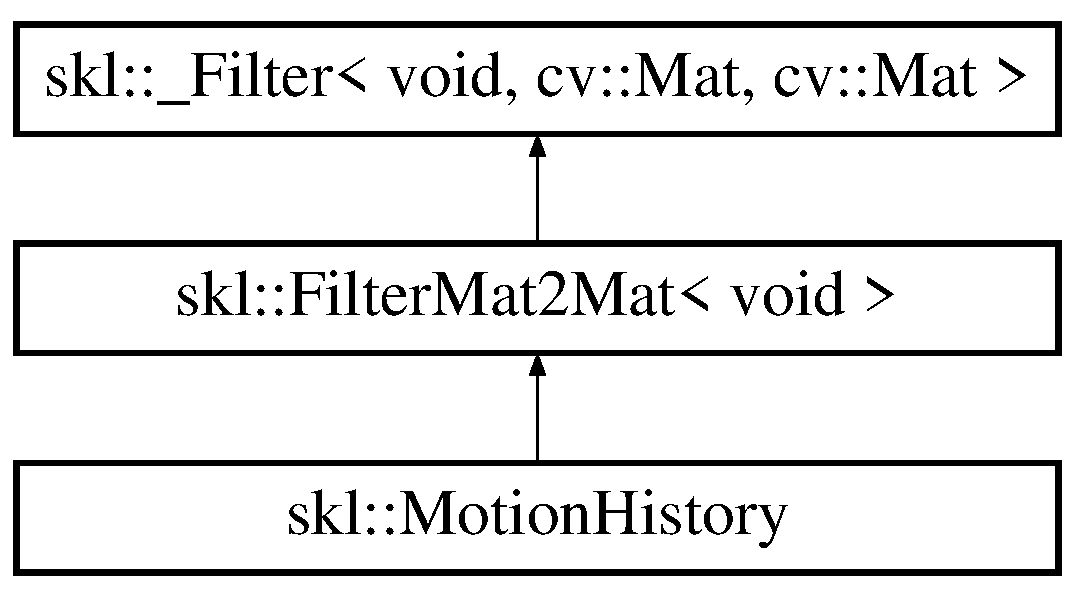
\includegraphics[height=3.000000cm]{classskl_1_1_motion_history}
\end{center}
\end{figure}
\subsection*{Public Member Functions}
\begin{DoxyCompactItemize}
\item 
\hypertarget{classskl_1_1_motion_history_ac6a775109ea17ab2faef96b81fb6af7f}{}\label{classskl_1_1_motion_history_ac6a775109ea17ab2faef96b81fb6af7f} 
\hyperlink{classskl_1_1_motion_history_ac6a775109ea17ab2faef96b81fb6af7f}{Motion\+History} (int history\+\_\+length=8)
\begin{DoxyCompactList}\small\item\em デフォルトコンストラクタ \end{DoxyCompactList}\item 
\hypertarget{classskl_1_1_motion_history_a96663c59d447b957a2119b88d19ba3ef}{}\label{classskl_1_1_motion_history_a96663c59d447b957a2119b88d19ba3ef} 
virtual \hyperlink{classskl_1_1_motion_history_a96663c59d447b957a2119b88d19ba3ef}{$\sim$\+Motion\+History} ()
\begin{DoxyCompactList}\small\item\em デストラクタ \end{DoxyCompactList}\item 
\hypertarget{classskl_1_1_motion_history_a989d3ca9c62b0e2f54049e2c80d9b812}{}\label{classskl_1_1_motion_history_a989d3ca9c62b0e2f54049e2c80d9b812} 
void {\bfseries clear} ()
\item 
\hypertarget{classskl_1_1_motion_history_a1b4139e0548de8186a6d8ff5eb12ad2a}{}\label{classskl_1_1_motion_history_a1b4139e0548de8186a6d8ff5eb12ad2a} 
void {\bfseries compute} (const cv\+::\+Mat \&mask)
\item 
\hypertarget{classskl_1_1_motion_history_af4e461272b6055e96a7577f320ae1c4b}{}\label{classskl_1_1_motion_history_af4e461272b6055e96a7577f320ae1c4b} 
void {\bfseries compute} (const cv\+::\+Mat \&mask, cv\+::\+Mat \&dest)
\item 
\hypertarget{classskl_1_1_motion_history_a4f9e603fbd0b3f7eaf31b5dd6dbbf692}{}\label{classskl_1_1_motion_history_a4f9e603fbd0b3f7eaf31b5dd6dbbf692} 
const cv\+::\+Mat \& {\bfseries motion\+\_\+history\+\_\+image} () const
\item 
\hypertarget{classskl_1_1_motion_history_a5fb7cb9051242af9a3c23515332c6733}{}\label{classskl_1_1_motion_history_a5fb7cb9051242af9a3c23515332c6733} 
int {\bfseries history\+\_\+length} () const
\item 
\hypertarget{classskl_1_1_motion_history_a034de06af6715ba26cd7f9dd90ceaf6d}{}\label{classskl_1_1_motion_history_a034de06af6715ba26cd7f9dd90ceaf6d} 
void {\bfseries history\+\_\+length} (int \+\_\+\+\_\+history\+\_\+length)
\end{DoxyCompactItemize}
\subsection*{Protected Attributes}
\begin{DoxyCompactItemize}
\item 
\hypertarget{classskl_1_1_motion_history_a81237db3cea6a809e9c1f2a64d43f900}{}\label{classskl_1_1_motion_history_a81237db3cea6a809e9c1f2a64d43f900} 
int {\bfseries step}
\item 
\hypertarget{classskl_1_1_motion_history_a08d378704fe9fe7e2791519e36ea82b7}{}\label{classskl_1_1_motion_history_a08d378704fe9fe7e2791519e36ea82b7} 
unsigned char {\bfseries offset}
\item 
\hypertarget{classskl_1_1_motion_history_a824a5cdfecf636cc6a7ff8ef53142575}{}\label{classskl_1_1_motion_history_a824a5cdfecf636cc6a7ff8ef53142575} 
cv\+::\+Mat {\bfseries prev}
\item 
\hypertarget{classskl_1_1_motion_history_a74ca6f44b70d17ee8548e263b366e463}{}\label{classskl_1_1_motion_history_a74ca6f44b70d17ee8548e263b366e463} 
cv\+::\+Size {\bfseries size}
\end{DoxyCompactItemize}


\subsection{Detailed Description}
Motion\+History\+Imageを作る 

The documentation for this class was generated from the following files\+:\begin{DoxyCompactItemize}
\item 
Open\+C\+V/include/\hyperlink{_motion_history_8h}{Motion\+History.\+h}\item 
Open\+C\+V/src/\hyperlink{_motion_history_8cpp}{Motion\+History.\+cpp}\end{DoxyCompactItemize}

\hypertarget{structskl_1_1_mouse_event}{}\section{skl\+:\+:Mouse\+Event Struct Reference}
\label{structskl_1_1_mouse_event}\index{skl\+::\+Mouse\+Event@{skl\+::\+Mouse\+Event}}
\subsection*{Public Attributes}
\begin{DoxyCompactItemize}
\item 
\hypertarget{structskl_1_1_mouse_event_a85cc97d2e7f40d575a9c663565c9c1f4}{}\label{structskl_1_1_mouse_event_a85cc97d2e7f40d575a9c663565c9c1f4} 
int {\bfseries type}
\item 
\hypertarget{structskl_1_1_mouse_event_ae2f57097fb934e8581ed048520aa248a}{}\label{structskl_1_1_mouse_event_ae2f57097fb934e8581ed048520aa248a} 
int {\bfseries flag}
\item 
\hypertarget{structskl_1_1_mouse_event_a5cb63b13fca08b0981c34475b5ab383a}{}\label{structskl_1_1_mouse_event_a5cb63b13fca08b0981c34475b5ab383a} 
cv\+::\+Point {\bfseries location}
\end{DoxyCompactItemize}


The documentation for this struct was generated from the following file\+:\begin{DoxyCompactItemize}
\item 
Open\+C\+V/include/\hyperlink{_cv_mouse_event_handler_8h}{Cv\+Mouse\+Event\+Handler.\+h}\end{DoxyCompactItemize}

\hypertarget{classskl_1_1_object_state}{}\section{skl\+:\+:Object\+State Class Reference}
\label{classskl_1_1_object_state}\index{skl\+::\+Object\+State@{skl\+::\+Object\+State}}
Inheritance diagram for skl\+:\+:Object\+State\+:\begin{figure}[H]
\begin{center}
\leavevmode
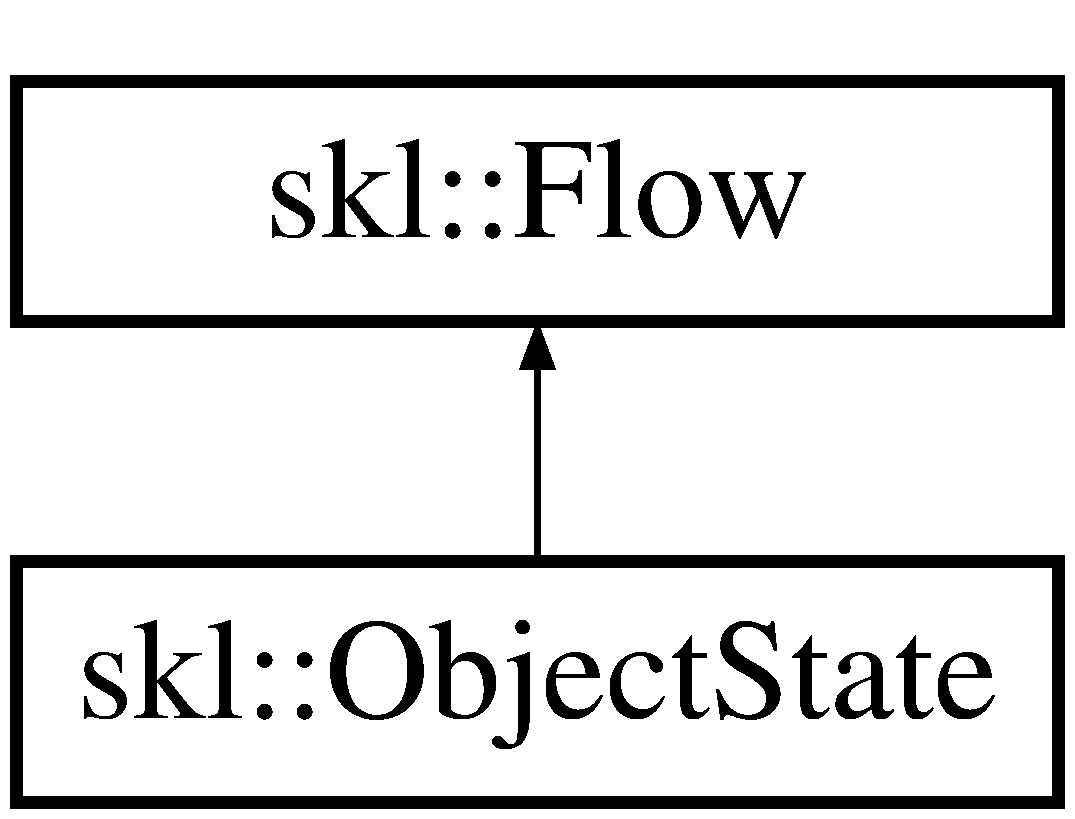
\includegraphics[height=2.000000cm]{classskl_1_1_object_state}
\end{center}
\end{figure}
\subsection*{Public Types}
\begin{DoxyCompactItemize}
\item 
\hypertarget{classskl_1_1_object_state_ae78add76688604bf19f221cf84df44b6}{}\label{classskl_1_1_object_state_ae78add76688604bf19f221cf84df44b6} 
enum {\bfseries Handling\+State} \{ {\bfseries N\+O\+T\+\_\+\+H\+A\+N\+D\+L\+ED} =0, 
{\bfseries H\+A\+N\+D\+L\+ED} = 1
 \}
\end{DoxyCompactItemize}
\subsection*{Public Member Functions}
\begin{DoxyCompactItemize}
\item 
\hypertarget{classskl_1_1_object_state_a3bc97a3a7493cbef68d9442e3e0711e5}{}\label{classskl_1_1_object_state_a3bc97a3a7493cbef68d9442e3e0711e5} 
\hyperlink{classskl_1_1_object_state_a3bc97a3a7493cbef68d9442e3e0711e5}{Object\+State} (int location\+\_\+resolution=S\+K\+L\+\_\+\+L\+O\+C\+A\+T\+I\+O\+N\+\_\+\+R\+E\+S\+O\+L\+U\+T\+I\+O\+N\+\_\+\+D\+E\+F\+A\+U\+LT)
\begin{DoxyCompactList}\small\item\em デフォルトコンストラクタ \end{DoxyCompactList}\item 
\hypertarget{classskl_1_1_object_state_a622db4af996ce80f6b4fd4f3b788a876}{}\label{classskl_1_1_object_state_a622db4af996ce80f6b4fd4f3b788a876} 
\hyperlink{classskl_1_1_object_state_a622db4af996ce80f6b4fd4f3b788a876}{Object\+State} (const \hyperlink{classskl_1_1_flow}{Flow} \&other)
\begin{DoxyCompactList}\small\item\em 他のインスタンスからのコンストラクタ.\+Shallow Copyであることに注意 \end{DoxyCompactList}\item 
\hypertarget{classskl_1_1_object_state_a4a6f7317a6fa42f6080b38573d205373}{}\label{classskl_1_1_object_state_a4a6f7317a6fa42f6080b38573d205373} 
virtual \hyperlink{classskl_1_1_object_state_a4a6f7317a6fa42f6080b38573d205373}{$\sim$\+Object\+State} ()
\begin{DoxyCompactList}\small\item\em デストラクタ \end{DoxyCompactList}\item 
\hypertarget{classskl_1_1_object_state_a4be418599ae600c7e3beeeaddf69e44a}{}\label{classskl_1_1_object_state_a4be418599ae600c7e3beeeaddf69e44a} 
\hyperlink{classskl_1_1_object_state}{Object\+State} \& {\bfseries operator=} (const \hyperlink{classskl_1_1_object_state}{Object\+State} \&other)
\item 
\hypertarget{classskl_1_1_object_state_ab74af07c26fc335bd43ee486475cad13}{}\label{classskl_1_1_object_state_ab74af07c26fc335bd43ee486475cad13} 
cv\+::\+Point {\bfseries argmax\+\_\+location} (Handling\+State h) const
\item 
\hypertarget{classskl_1_1_object_state_afd29f207af856e1a00a9d957d2296316}{}\label{classskl_1_1_object_state_afd29f207af856e1a00a9d957d2296316} 
cv\+::\+Point {\bfseries argmax\+\_\+location} () const
\item 
\hypertarget{classskl_1_1_object_state_a39fa0da0d058be0daf30b4cda4025dae}{}\label{classskl_1_1_object_state_a39fa0da0d058be0daf30b4cda4025dae} 
cv\+::\+Point {\bfseries argmax\+\_\+location} (Handling\+State h, float \&prob) const
\item 
\hypertarget{classskl_1_1_object_state_a8bc3f2ac6f88a460f244d6f64d437603}{}\label{classskl_1_1_object_state_a8bc3f2ac6f88a460f244d6f64d437603} 
cv\+::\+Point {\bfseries argmax\+\_\+location} (float \&prob) const
\item 
\hypertarget{classskl_1_1_object_state_a23a03a3bd6eeff791756cdc0cddc00ad}{}\label{classskl_1_1_object_state_a23a03a3bd6eeff791756cdc0cddc00ad} 
float {\bfseries prob\+Handling\+State} (Handling\+State h) const
\item 
\hypertarget{classskl_1_1_object_state_af9c33e4dc0a97aa12097585e581799ca}{}\label{classskl_1_1_object_state_af9c33e4dc0a97aa12097585e581799ca} 
int {\bfseries resolution} () const
\item 
\hypertarget{classskl_1_1_object_state_ac1f11d384a0abe08b432e52365cedb5d}{}\label{classskl_1_1_object_state_ac1f11d384a0abe08b432e52365cedb5d} 
const cv\+::\+Mat \& {\bfseries location} (Handling\+State h\+\_\+state) const
\item 
\hypertarget{classskl_1_1_object_state_a7d955879826351089d98bac30604c9dd}{}\label{classskl_1_1_object_state_a7d955879826351089d98bac30604c9dd} 
cv\+::\+Mat \& {\bfseries location} (Handling\+State h\+\_\+state)
\item 
\hypertarget{classskl_1_1_object_state_a96dddb1afb7508618cefc07cf1dd8894}{}\label{classskl_1_1_object_state_a96dddb1afb7508618cefc07cf1dd8894} 
const cv\+::\+Mat \& {\bfseries operator\mbox{[}$\,$\mbox{]}} (Handling\+State h) const
\item 
\hypertarget{classskl_1_1_object_state_a0c7b27f3a691a1002e8701adfff0bc8e}{}\label{classskl_1_1_object_state_a0c7b27f3a691a1002e8701adfff0bc8e} 
cv\+::\+Mat \& {\bfseries operator\mbox{[}$\,$\mbox{]}} (Handling\+State h)
\end{DoxyCompactItemize}
\subsection*{Additional Inherited Members}


The documentation for this class was generated from the following files\+:\begin{DoxyCompactItemize}
\item 
Open\+C\+V/include/\hyperlink{_object_state_8h}{Object\+State.\+h}\item 
Open\+C\+V/src/\hyperlink{_object_state_8cpp}{Object\+State.\+cpp}\end{DoxyCompactItemize}

\hypertarget{classskl_1_1_opt_parser}{}\section{skl\+:\+:Opt\+Parser Class Reference}
\label{classskl_1_1_opt_parser}\index{skl\+::\+Opt\+Parser@{skl\+::\+Opt\+Parser}}


Parse Option from Command\+Line.  




{\ttfamily \#include $<$Opt\+Parser.\+h$>$}

\subsection*{Public Member Functions}
\begin{DoxyCompactItemize}
\item 
\hypertarget{classskl_1_1_opt_parser_ab8720ec621a124e68046a31c85405d1d}{}\label{classskl_1_1_opt_parser_ab8720ec621a124e68046a31c85405d1d} 
\hyperlink{classskl_1_1_opt_parser_ab8720ec621a124e68046a31c85405d1d}{Opt\+Parser} (const std\+::string \&conf\+\_\+deliminator=\char`\"{}\+:\char`\"{})
\begin{DoxyCompactList}\small\item\em デフォルトコンストラクタ \end{DoxyCompactList}\item 
\hypertarget{classskl_1_1_opt_parser_afda19cef607451fa8bddeeff1be0f1a2}{}\label{classskl_1_1_opt_parser_afda19cef607451fa8bddeeff1be0f1a2} 
virtual \hyperlink{classskl_1_1_opt_parser_afda19cef607451fa8bddeeff1be0f1a2}{$\sim$\+Opt\+Parser} ()
\begin{DoxyCompactList}\small\item\em デストラクタ \end{DoxyCompactList}\item 
\hypertarget{classskl_1_1_opt_parser_a5b035092633240161519545cca3534a1}{}\label{classskl_1_1_opt_parser_a5b035092633240161519545cca3534a1} 
void {\bfseries on} (const std\+::string \&long\+\_\+form, const std\+::string \&expression, const std\+::string \&explanation)
\item 
\hypertarget{classskl_1_1_opt_parser_aaad7fee81b7d17ffe0672161d61a31cf}{}\label{classskl_1_1_opt_parser_aaad7fee81b7d17ffe0672161d61a31cf} 
void {\bfseries on} (const std\+::string \&short\+\_\+form, const std\+::string \&long\+\_\+form, const std\+::string \&expression, const std\+::string \&explanation)
\item 
\hypertarget{classskl_1_1_opt_parser_aa0cdaff6ce699507675bf17debdb37c1}{}\label{classskl_1_1_opt_parser_aa0cdaff6ce699507675bf17debdb37c1} 
bool {\bfseries get} (const std\+::string \&var\+\_\+name, std\+::string $\ast$var) const
\item 
\hypertarget{classskl_1_1_opt_parser_a97bc22822e584f3766a35b089b47ab96}{}\label{classskl_1_1_opt_parser_a97bc22822e584f3766a35b089b47ab96} 
std\+::vector$<$ std\+::string $>$ {\bfseries parse} (int argc, char $\ast$argv\mbox{[}$\,$\mbox{]})
\item 
\hypertarget{classskl_1_1_opt_parser_a5f4ca7a65af552f6b2d14b89efdf4a9c}{}\label{classskl_1_1_opt_parser_a5f4ca7a65af552f6b2d14b89efdf4a9c} 
std\+::vector$<$ std\+::string $>$ {\bfseries parse} (const std\+::vector$<$ std\+::string $>$ \&args)
\item 
\hypertarget{classskl_1_1_opt_parser_a051739884bbb805d84ac301da7c93673}{}\label{classskl_1_1_opt_parser_a051739884bbb805d84ac301da7c93673} 
void {\bfseries usage} () const
\item 
\hypertarget{classskl_1_1_opt_parser_af22343fc946d98c029e8699b9e15abf2}{}\label{classskl_1_1_opt_parser_af22343fc946d98c029e8699b9e15abf2} 
bool {\bfseries help} () const
\end{DoxyCompactItemize}
\subsection*{Protected Member Functions}
\begin{DoxyCompactItemize}
\item 
\hypertarget{classskl_1_1_opt_parser_a07d5d90a99e9c3058d245f1d79939e1e}{}\label{classskl_1_1_opt_parser_a07d5d90a99e9c3058d245f1d79939e1e} 
int {\bfseries check\+Type} (const std\+::string \&str) const
\end{DoxyCompactItemize}
\subsection*{Static Protected Member Functions}
\begin{DoxyCompactItemize}
\item 
\hypertarget{classskl_1_1_opt_parser_acd1bb930b4330c4d29a294537b874f01}{}\label{classskl_1_1_opt_parser_acd1bb930b4330c4d29a294537b874f01} 
static void {\bfseries parse\+\_\+short\+\_\+form} (const std\+::string \&form, std\+::string $\ast$var\+\_\+name)
\item 
\hypertarget{classskl_1_1_opt_parser_ab56f6bdd5af0b74ce57ef739fe6f7671}{}\label{classskl_1_1_opt_parser_ab56f6bdd5af0b74ce57ef739fe6f7671} 
static void {\bfseries parse\+\_\+long\+\_\+form} (const std\+::string \&form, std\+::string $\ast$var\+\_\+name)
\item 
\hypertarget{classskl_1_1_opt_parser_a33940c3ac37e2493bf0f4b0e3808794f}{}\label{classskl_1_1_opt_parser_a33940c3ac37e2493bf0f4b0e3808794f} 
static std\+::string {\bfseries get\+\_\+short\+\_\+form} (const std\+::string \&str)
\item 
\hypertarget{classskl_1_1_opt_parser_a4204efe57580846f70fffbd9a6323569}{}\label{classskl_1_1_opt_parser_a4204efe57580846f70fffbd9a6323569} 
static std\+::string {\bfseries get\+\_\+long\+\_\+form} (const std\+::string \&str)
\item 
\hypertarget{classskl_1_1_opt_parser_a712f0d6b2d077b45651b252bc6b12da2}{}\label{classskl_1_1_opt_parser_a712f0d6b2d077b45651b252bc6b12da2} 
static std\+::string {\bfseries make\+\_\+usage} (const std\+::string \&short\+\_\+name, const std\+::string \&var\+\_\+name, const std\+::string \&expression, const std\+::string \&explanation)
\end{DoxyCompactItemize}
\subsection*{Protected Attributes}
\begin{DoxyCompactItemize}
\item 
\hypertarget{classskl_1_1_opt_parser_a185db13bf585b6064d5c8829484655c4}{}\label{classskl_1_1_opt_parser_a185db13bf585b6064d5c8829484655c4} 
std\+::map$<$ std\+::string, std\+::string $>$ {\bfseries explanations}
\item 
\hypertarget{classskl_1_1_opt_parser_acfc5e5e788691729aa4c491a531d6f26}{}\label{classskl_1_1_opt_parser_acfc5e5e788691729aa4c491a531d6f26} 
std\+::map$<$ std\+::string, std\+::string $>$ {\bfseries option\+\_\+values}
\item 
\hypertarget{classskl_1_1_opt_parser_a283fca12ae09d559e337a725c54e9623}{}\label{classskl_1_1_opt_parser_a283fca12ae09d559e337a725c54e9623} 
std\+::map$<$ std\+::string, std\+::string $>$ {\bfseries short\+\_\+long\+\_\+map}
\item 
\hypertarget{classskl_1_1_opt_parser_a212dd7ecb4ed3c5175866a3b6df3b365}{}\label{classskl_1_1_opt_parser_a212dd7ecb4ed3c5175866a3b6df3b365} 
std\+::string {\bfseries conf\+\_\+deliminator}
\item 
\hypertarget{classskl_1_1_opt_parser_a2f60d7aa1373b2682e2b524bfd34992e}{}\label{classskl_1_1_opt_parser_a2f60d7aa1373b2682e2b524bfd34992e} 
bool {\bfseries \+\_\+help}
\end{DoxyCompactItemize}


\subsection{Detailed Description}
Parse Option from Command\+Line. 

The documentation for this class was generated from the following files\+:\begin{DoxyCompactItemize}
\item 
Core/include/\hyperlink{_opt_parser_8h}{Opt\+Parser.\+h}\item 
Core/src/\hyperlink{_opt_parser_8cpp}{Opt\+Parser.\+cpp}\end{DoxyCompactItemize}

\hypertarget{classskl_1_1_opt_parser_atom}{}\section{skl\+:\+:Opt\+Parser\+Atom$<$ T $>$ Class Template Reference}
\label{classskl_1_1_opt_parser_atom}\index{skl\+::\+Opt\+Parser\+Atom$<$ T $>$@{skl\+::\+Opt\+Parser\+Atom$<$ T $>$}}
Inheritance diagram for skl\+:\+:Opt\+Parser\+Atom$<$ T $>$\+:\begin{figure}[H]
\begin{center}
\leavevmode
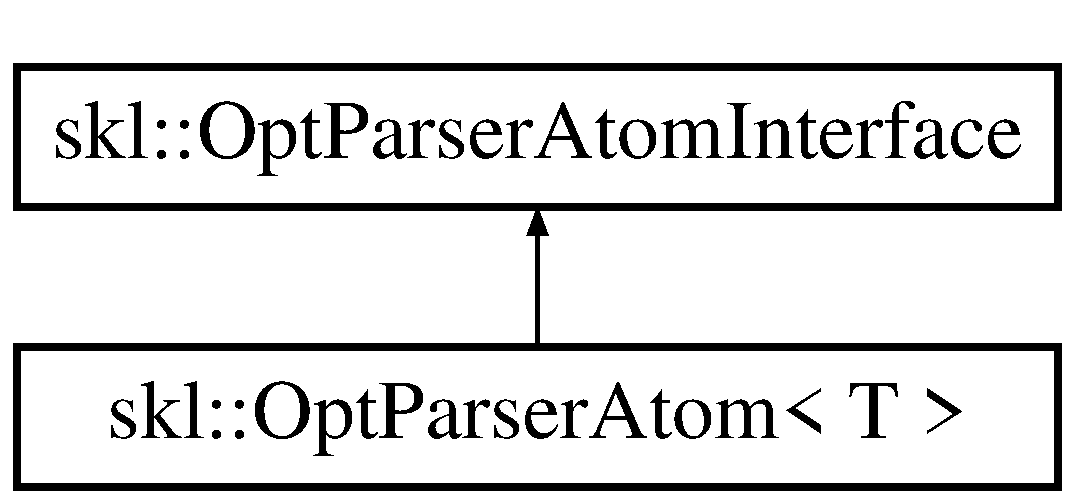
\includegraphics[height=2.000000cm]{classskl_1_1_opt_parser_atom}
\end{center}
\end{figure}
\subsection*{Public Member Functions}
\begin{DoxyCompactItemize}
\item 
\hypertarget{classskl_1_1_opt_parser_atom_a8a7f6fb8e4ffdcbc7bb3e8d38e1ca98d}{}\label{classskl_1_1_opt_parser_atom_a8a7f6fb8e4ffdcbc7bb3e8d38e1ca98d} 
{\bfseries Opt\+Parser\+Atom} (const std\+::string \&short\+\_\+form, const std\+::string \&var\+\_\+name, const std\+::string \&expression, const std\+::string \&explanation, T $\ast$dest)
\item 
\hypertarget{classskl_1_1_opt_parser_atom_acdf3f38281c75daf8fd5828f94746747}{}\label{classskl_1_1_opt_parser_atom_acdf3f38281c75daf8fd5828f94746747} 
void {\bfseries on} (\hyperlink{classskl_1_1_opt_parser}{Opt\+Parser} $\ast$parser)
\item 
\hypertarget{classskl_1_1_opt_parser_atom_a06ad48ea0c67af986c4fb906c2f58c77}{}\label{classskl_1_1_opt_parser_atom_a06ad48ea0c67af986c4fb906c2f58c77} 
void {\bfseries get} (\hyperlink{classskl_1_1_opt_parser}{Opt\+Parser} $\ast$parser)
\end{DoxyCompactItemize}
\subsection*{Protected Attributes}
\begin{DoxyCompactItemize}
\item 
\hypertarget{classskl_1_1_opt_parser_atom_a5bc2ca7397229a0b0bed0134e8fa5b50}{}\label{classskl_1_1_opt_parser_atom_a5bc2ca7397229a0b0bed0134e8fa5b50} 
std\+::string {\bfseries short\+\_\+form}
\item 
\hypertarget{classskl_1_1_opt_parser_atom_a3113456fdb4df8a077e28993796d7291}{}\label{classskl_1_1_opt_parser_atom_a3113456fdb4df8a077e28993796d7291} 
std\+::string {\bfseries var\+\_\+name}
\item 
\hypertarget{classskl_1_1_opt_parser_atom_aa49aaaff1827f1085d24c246fa7f7c9b}{}\label{classskl_1_1_opt_parser_atom_aa49aaaff1827f1085d24c246fa7f7c9b} 
std\+::string {\bfseries expression}
\item 
\hypertarget{classskl_1_1_opt_parser_atom_aa741566483011d0be3d54653c4dde021}{}\label{classskl_1_1_opt_parser_atom_aa741566483011d0be3d54653c4dde021} 
std\+::string {\bfseries explanation}
\item 
\hypertarget{classskl_1_1_opt_parser_atom_af7a2921f7da6dd1981ce4ac791176448}{}\label{classskl_1_1_opt_parser_atom_af7a2921f7da6dd1981ce4ac791176448} 
T $\ast$ {\bfseries dest}
\end{DoxyCompactItemize}
\subsection*{Additional Inherited Members}


The documentation for this class was generated from the following file\+:\begin{DoxyCompactItemize}
\item 
Core/include/\hyperlink{_opt_parser_8h}{Opt\+Parser.\+h}\end{DoxyCompactItemize}

\hypertarget{classskl_1_1_opt_parser_atom_container}{}\section{skl\+:\+:Opt\+Parser\+Atom\+Container$<$ T, Container $>$ Class Template Reference}
\label{classskl_1_1_opt_parser_atom_container}\index{skl\+::\+Opt\+Parser\+Atom\+Container$<$ T, Container $>$@{skl\+::\+Opt\+Parser\+Atom\+Container$<$ T, Container $>$}}
Inheritance diagram for skl\+:\+:Opt\+Parser\+Atom\+Container$<$ T, Container $>$\+:\begin{figure}[H]
\begin{center}
\leavevmode
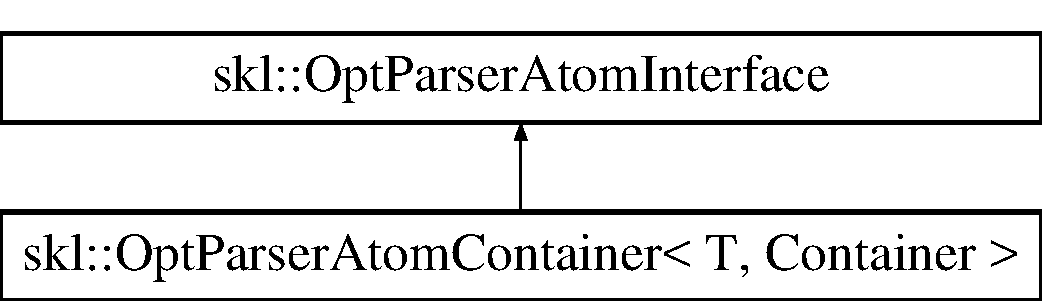
\includegraphics[height=2.000000cm]{classskl_1_1_opt_parser_atom_container}
\end{center}
\end{figure}
\subsection*{Public Member Functions}
\begin{DoxyCompactItemize}
\item 
\hypertarget{classskl_1_1_opt_parser_atom_container_ae641a31bccdd30ef9d39c23e85064a56}{}\label{classskl_1_1_opt_parser_atom_container_ae641a31bccdd30ef9d39c23e85064a56} 
{\bfseries Opt\+Parser\+Atom\+Container} (const std\+::string \&short\+\_\+form, const std\+::string \&var\+\_\+name, const std\+::string \&default\+\_\+value, const std\+::string \&expression, const std\+::string \&explanation, Container $\ast$dest, const std\+::string \&deliminator=\char`\"{}\+:\char`\"{}, int length=-\/1)
\item 
\hypertarget{classskl_1_1_opt_parser_atom_container_a739477fc4eb8ff79384671887adfb3eb}{}\label{classskl_1_1_opt_parser_atom_container_a739477fc4eb8ff79384671887adfb3eb} 
void {\bfseries on} (\hyperlink{classskl_1_1_opt_parser}{Opt\+Parser} $\ast$parser)
\item 
\hypertarget{classskl_1_1_opt_parser_atom_container_a41919b3684566bf4cea0c97f309a4b5f}{}\label{classskl_1_1_opt_parser_atom_container_a41919b3684566bf4cea0c97f309a4b5f} 
void {\bfseries get} (\hyperlink{classskl_1_1_opt_parser}{Opt\+Parser} $\ast$parser)
\item 
\hypertarget{classskl_1_1_opt_parser_atom_container_ae6df89d2c33874c413223afcca62b350}{}\label{classskl_1_1_opt_parser_atom_container_ae6df89d2c33874c413223afcca62b350} 
void {\bfseries set\+\_\+default} ()
\end{DoxyCompactItemize}
\subsection*{Protected Attributes}
\begin{DoxyCompactItemize}
\item 
\hypertarget{classskl_1_1_opt_parser_atom_container_a5d33e33b274d5dcd992eea5c697d22db}{}\label{classskl_1_1_opt_parser_atom_container_a5d33e33b274d5dcd992eea5c697d22db} 
std\+::string {\bfseries short\+\_\+form}
\item 
\hypertarget{classskl_1_1_opt_parser_atom_container_a23b8ab845d674477c4e246096c205e42}{}\label{classskl_1_1_opt_parser_atom_container_a23b8ab845d674477c4e246096c205e42} 
std\+::string {\bfseries var\+\_\+name}
\item 
\hypertarget{classskl_1_1_opt_parser_atom_container_a2f0e19983f3d60b3692fee7efa2e34ad}{}\label{classskl_1_1_opt_parser_atom_container_a2f0e19983f3d60b3692fee7efa2e34ad} 
std\+::string {\bfseries default\+\_\+value}
\item 
\hypertarget{classskl_1_1_opt_parser_atom_container_a4e79b705199c2e715b8f7329d9979813}{}\label{classskl_1_1_opt_parser_atom_container_a4e79b705199c2e715b8f7329d9979813} 
std\+::string {\bfseries expression}
\item 
\hypertarget{classskl_1_1_opt_parser_atom_container_ad7c55f9221f17b5f9c8f53d62237425f}{}\label{classskl_1_1_opt_parser_atom_container_ad7c55f9221f17b5f9c8f53d62237425f} 
std\+::string {\bfseries explanation}
\item 
\hypertarget{classskl_1_1_opt_parser_atom_container_ae0b8d86db2a02d66b903f159268ab4ac}{}\label{classskl_1_1_opt_parser_atom_container_ae0b8d86db2a02d66b903f159268ab4ac} 
Container $\ast$ {\bfseries dest}
\item 
\hypertarget{classskl_1_1_opt_parser_atom_container_a1073f927eb5201a93888612088bb3e08}{}\label{classskl_1_1_opt_parser_atom_container_a1073f927eb5201a93888612088bb3e08} 
std\+::string {\bfseries deliminator}
\item 
\hypertarget{classskl_1_1_opt_parser_atom_container_ae8da8fced77c408c406fd754bb374b1e}{}\label{classskl_1_1_opt_parser_atom_container_ae8da8fced77c408c406fd754bb374b1e} 
int {\bfseries length}
\end{DoxyCompactItemize}
\subsection*{Additional Inherited Members}


The documentation for this class was generated from the following file\+:\begin{DoxyCompactItemize}
\item 
Core/include/\hyperlink{_opt_parser_8h}{Opt\+Parser.\+h}\end{DoxyCompactItemize}

\hypertarget{classskl_1_1_opt_parser_atom_interface}{}\section{skl\+:\+:Opt\+Parser\+Atom\+Interface Class Reference}
\label{classskl_1_1_opt_parser_atom_interface}\index{skl\+::\+Opt\+Parser\+Atom\+Interface@{skl\+::\+Opt\+Parser\+Atom\+Interface}}
Inheritance diagram for skl\+:\+:Opt\+Parser\+Atom\+Interface\+:\begin{figure}[H]
\begin{center}
\leavevmode
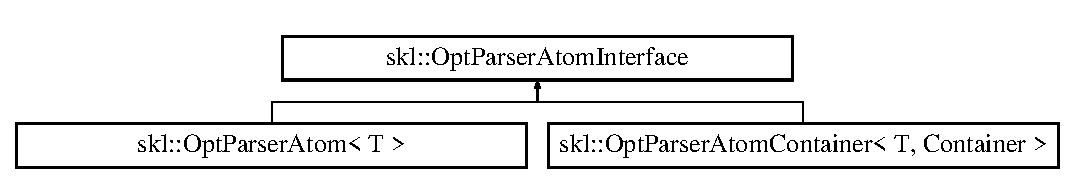
\includegraphics[height=2.000000cm]{classskl_1_1_opt_parser_atom_interface}
\end{center}
\end{figure}
\subsection*{Public Member Functions}
\begin{DoxyCompactItemize}
\item 
\hypertarget{classskl_1_1_opt_parser_atom_interface_a4326bc85c2f177e52f530a0b10ec1fec}{}\label{classskl_1_1_opt_parser_atom_interface_a4326bc85c2f177e52f530a0b10ec1fec} 
virtual void {\bfseries on} (\hyperlink{classskl_1_1_opt_parser}{Opt\+Parser} $\ast$parser)=0
\item 
\hypertarget{classskl_1_1_opt_parser_atom_interface_af54d653154f8f8183ca356e04328cea8}{}\label{classskl_1_1_opt_parser_atom_interface_af54d653154f8f8183ca356e04328cea8} 
virtual void {\bfseries get} (\hyperlink{classskl_1_1_opt_parser}{Opt\+Parser} $\ast$parser)=0
\end{DoxyCompactItemize}
\subsection*{Public Attributes}
\begin{DoxyCompactItemize}
\item 
\hypertarget{classskl_1_1_opt_parser_atom_interface_a6bc8353a1cd5a05bb2330474a721d14f}{}\label{classskl_1_1_opt_parser_atom_interface_a6bc8353a1cd5a05bb2330474a721d14f} 
\hyperlink{classskl_1_1_opt_parser_atom_interface}{Opt\+Parser\+Atom\+Interface} $\ast$ {\bfseries next}
\end{DoxyCompactItemize}
\subsection*{Static Public Attributes}
\begin{DoxyCompactItemize}
\item 
\hypertarget{classskl_1_1_opt_parser_atom_interface_a5578648ddb5d70b020e126adc523d202}{}\label{classskl_1_1_opt_parser_atom_interface_a5578648ddb5d70b020e126adc523d202} 
static \hyperlink{classskl_1_1_opt_parser_atom_interface}{Opt\+Parser\+Atom\+Interface} $\ast$ {\bfseries atom\+\_\+top} = N\+U\+LL
\end{DoxyCompactItemize}


The documentation for this class was generated from the following files\+:\begin{DoxyCompactItemize}
\item 
Core/include/\hyperlink{_opt_parser_8h}{Opt\+Parser.\+h}\item 
Core/src/\hyperlink{_opt_parser_8cpp}{Opt\+Parser.\+cpp}\end{DoxyCompactItemize}

\hypertarget{classskl_1_1_parallel_add_gradient_heterogenuity}{}\section{skl\+:\+:Parallel\+Add\+Gradient\+Heterogenuity Class Reference}
\label{classskl_1_1_parallel_add_gradient_heterogenuity}\index{skl\+::\+Parallel\+Add\+Gradient\+Heterogenuity@{skl\+::\+Parallel\+Add\+Gradient\+Heterogenuity}}
\subsection*{Public Member Functions}
\begin{DoxyCompactItemize}
\item 
\hypertarget{classskl_1_1_parallel_add_gradient_heterogenuity_a85b164b06a685548f6f6b7e106aa1fa7}{}\label{classskl_1_1_parallel_add_gradient_heterogenuity_a85b164b06a685548f6f6b7e106aa1fa7} 
{\bfseries Parallel\+Add\+Gradient\+Heterogenuity} (const cv\+::\+Mat \&data\+\_\+term, const cv\+::\+Mat \&gradient\+\_\+heterogenuity, cv\+::\+Mat \&smoothing\+\_\+term\+\_\+x, cv\+::\+Mat \&smoothing\+\_\+term\+\_\+y, float smoothing\+\_\+term\+\_\+weight)
\item 
\hypertarget{classskl_1_1_parallel_add_gradient_heterogenuity_a85da87e245322013360fea2232e161b9}{}\label{classskl_1_1_parallel_add_gradient_heterogenuity_a85da87e245322013360fea2232e161b9} 
void {\bfseries operator()} (const cv\+::\+Blocked\+Range \&range) const
\item 
\hypertarget{classskl_1_1_parallel_add_gradient_heterogenuity_aabafc3b922fcd0809692c2b187bb9134}{}\label{classskl_1_1_parallel_add_gradient_heterogenuity_aabafc3b922fcd0809692c2b187bb9134} 
int {\bfseries calc\+Data\+Term\+Penalty} (int val) const
\end{DoxyCompactItemize}
\subsection*{Protected Attributes}
\begin{DoxyCompactItemize}
\item 
\hypertarget{classskl_1_1_parallel_add_gradient_heterogenuity_a0f44d68f3570ffddac3f19db27e70975}{}\label{classskl_1_1_parallel_add_gradient_heterogenuity_a0f44d68f3570ffddac3f19db27e70975} 
const cv\+::\+Mat \& {\bfseries data\+\_\+term}
\item 
\hypertarget{classskl_1_1_parallel_add_gradient_heterogenuity_acc07e5bd2e5b6cd1e79fdd69612aaccf}{}\label{classskl_1_1_parallel_add_gradient_heterogenuity_acc07e5bd2e5b6cd1e79fdd69612aaccf} 
const cv\+::\+Mat \& {\bfseries gradient\+\_\+heterogenuity}
\item 
\hypertarget{classskl_1_1_parallel_add_gradient_heterogenuity_a17765db83b342f0eb47d4bbf6b767b35}{}\label{classskl_1_1_parallel_add_gradient_heterogenuity_a17765db83b342f0eb47d4bbf6b767b35} 
cv\+::\+Mat \& {\bfseries smoothing\+\_\+term\+\_\+x}
\item 
\hypertarget{classskl_1_1_parallel_add_gradient_heterogenuity_aafa6aa99d6a4740d51d5426ed8028494}{}\label{classskl_1_1_parallel_add_gradient_heterogenuity_aafa6aa99d6a4740d51d5426ed8028494} 
cv\+::\+Mat \& {\bfseries smoothing\+\_\+term\+\_\+y}
\item 
\hypertarget{classskl_1_1_parallel_add_gradient_heterogenuity_ab048e3c50d479c3d802e95f90e5386e2}{}\label{classskl_1_1_parallel_add_gradient_heterogenuity_ab048e3c50d479c3d802e95f90e5386e2} 
float {\bfseries smoothing\+\_\+term\+\_\+weight}
\end{DoxyCompactItemize}


The documentation for this class was generated from the following files\+:\begin{DoxyCompactItemize}
\item 
Open\+C\+V/include/Tex\+Cut.\+h\item 
Open\+C\+V/src/Tex\+Cut.\+cpp\end{DoxyCompactItemize}

\hypertarget{classskl_1_1_parallel_blending}{}\section{skl\+:\+:Parallel\+Blending$<$ Elem\+Type, Weight\+Type $>$ Class Template Reference}
\label{classskl_1_1_parallel_blending}\index{skl\+::\+Parallel\+Blending$<$ Elem\+Type, Weight\+Type $>$@{skl\+::\+Parallel\+Blending$<$ Elem\+Type, Weight\+Type $>$}}
\subsection*{Public Member Functions}
\begin{DoxyCompactItemize}
\item 
\hypertarget{classskl_1_1_parallel_blending_acd87d25766dd761d368081adedddc3d8}{}\label{classskl_1_1_parallel_blending_acd87d25766dd761d368081adedddc3d8} 
{\bfseries Parallel\+Blending} (const cv\+::\+Mat \&src1, const cv\+::\+Mat \&src2, const cv\+::\+Mat \&mask, cv\+::\+Mat \&dest)
\item 
\hypertarget{classskl_1_1_parallel_blending_ad7109be1d417ef6b2348eeca533b00da}{}\label{classskl_1_1_parallel_blending_ad7109be1d417ef6b2348eeca533b00da} 
void {\bfseries operator()} (const cv\+::\+Blocked\+Range \&range) const
\end{DoxyCompactItemize}
\subsection*{Protected Attributes}
\begin{DoxyCompactItemize}
\item 
\hypertarget{classskl_1_1_parallel_blending_a29343b128d6fed39999113b68824b3c1}{}\label{classskl_1_1_parallel_blending_a29343b128d6fed39999113b68824b3c1} 
const cv\+::\+Mat \& {\bfseries src1}
\item 
\hypertarget{classskl_1_1_parallel_blending_ace5344e54ab8ae5c2fe519f8623bcbd6}{}\label{classskl_1_1_parallel_blending_ace5344e54ab8ae5c2fe519f8623bcbd6} 
const cv\+::\+Mat \& {\bfseries src2}
\item 
\hypertarget{classskl_1_1_parallel_blending_a356e7f2592a00abc49b64b20cca84eb9}{}\label{classskl_1_1_parallel_blending_a356e7f2592a00abc49b64b20cca84eb9} 
const cv\+::\+Mat \& {\bfseries mask}
\item 
\hypertarget{classskl_1_1_parallel_blending_a58e7a8004c3e7565f5eca3ca63bb07b7}{}\label{classskl_1_1_parallel_blending_a58e7a8004c3e7565f5eca3ca63bb07b7} 
cv\+::\+Mat \& {\bfseries dest}
\end{DoxyCompactItemize}


The documentation for this class was generated from the following file\+:\begin{DoxyCompactItemize}
\item 
Open\+C\+V/include/sklcvutils\+\_\+blending.\+h\end{DoxyCompactItemize}

\hypertarget{classskl_1_1_parallel_calc_edge_capacity}{}\section{skl\+:\+:Parallel\+Calc\+Edge\+Capacity Class Reference}
\label{classskl_1_1_parallel_calc_edge_capacity}\index{skl\+::\+Parallel\+Calc\+Edge\+Capacity@{skl\+::\+Parallel\+Calc\+Edge\+Capacity}}
\subsection*{Public Member Functions}
\begin{DoxyCompactItemize}
\item 
\hypertarget{classskl_1_1_parallel_calc_edge_capacity_a29c94dc3e4e2e7d1d58ab38e92b01dbb}{}\label{classskl_1_1_parallel_calc_edge_capacity_a29c94dc3e4e2e7d1d58ab38e92b01dbb} 
{\bfseries Parallel\+Calc\+Edge\+Capacity} (const std\+::vector$<$ cv\+::\+Mat $>$ \&src, const std\+::vector$<$ cv\+::\+Mat $>$ \&sobel\+\_\+x, const std\+::vector$<$ cv\+::\+Mat $>$ \&sobel\+\_\+y, const std\+::vector$<$ cv\+::\+Mat $>$ \&bg\+\_\+img, const std\+::vector$<$ cv\+::\+Mat $>$ \&bg\+\_\+sobel\+\_\+x, const std\+::vector$<$ cv\+::\+Mat $>$ \&bg\+\_\+sobel\+\_\+y, const std\+::vector$<$ float $>$ \&noise\+\_\+std\+\_\+dev, const std\+::vector$<$ float $>$ \&gh\+\_\+expectation, const std\+::vector$<$ float $>$ \&gh\+\_\+std\+\_\+dev, float alpha, float thresh\+\_\+tex\+\_\+diff, unsigned char over\+\_\+exposure\+\_\+thresh, unsigned char under\+\_\+exposure\+\_\+thresh, cv\+::\+Mat \&data\+\_\+term, cv\+::\+Mat \&gradient\+\_\+heterogenuity, cv\+::\+Mat \&smoothing\+\_\+term\+\_\+x, cv\+::\+Mat \&smoothing\+\_\+term\+\_\+y)
\item 
\hypertarget{classskl_1_1_parallel_calc_edge_capacity_a90870970fb881a8df7fefcffcb5b4871}{}\label{classskl_1_1_parallel_calc_edge_capacity_a90870970fb881a8df7fefcffcb5b4871} 
void {\bfseries operator()} (const cv\+::\+Blocked\+Range \&range) const
\end{DoxyCompactItemize}
\subsection*{Static Public Member Functions}
\begin{DoxyCompactItemize}
\item 
\hypertarget{classskl_1_1_parallel_calc_edge_capacity_ad4b59e6047dbce5350f77681aa9986ba}{}\label{classskl_1_1_parallel_calc_edge_capacity_ad4b59e6047dbce5350f77681aa9986ba} 
static float {\bfseries calc\+Grad\+Hetero} (std\+::vector$<$ float $>$ \&power)
\end{DoxyCompactItemize}
\subsection*{Protected Member Functions}
\begin{DoxyCompactItemize}
\item 
\hypertarget{classskl_1_1_parallel_calc_edge_capacity_aaad1201111c178f9459ad6e111e33fc8}{}\label{classskl_1_1_parallel_calc_edge_capacity_aaad1201111c178f9459ad6e111e33fc8} 
void {\bfseries calc\+Data\+Term} (const cv\+::\+Mat \&sobel\+\_\+x, const cv\+::\+Mat \&sobel\+\_\+y, const cv\+::\+Mat \&bg\+\_\+sobel\+\_\+x, const cv\+::\+Mat \&bg\+\_\+sobel\+\_\+y, float nsd, float gh\+\_\+mean, float gh\+\_\+sd, float $\ast$tex\+\_\+int, float $\ast$gh, float $\ast$tex\+\_\+diff) const
\item 
\hypertarget{classskl_1_1_parallel_calc_edge_capacity_a80cce5c0ac677f00ef0dde521ee5e43f}{}\label{classskl_1_1_parallel_calc_edge_capacity_a80cce5c0ac677f00ef0dde521ee5e43f} 
void {\bfseries calc\+Smoothing\+Term} (const cv\+::\+Mat \&src\+\_\+left, const cv\+::\+Mat \&src\+\_\+right, const cv\+::\+Mat \&bg\+\_\+left, const cv\+::\+Mat \&bg\+\_\+right, float $\ast$smoothing\+\_\+term, float nsd) const
\item 
\hypertarget{classskl_1_1_parallel_calc_edge_capacity_acf7a71128e015c39b2024d193239eb6d}{}\label{classskl_1_1_parallel_calc_edge_capacity_acf7a71128e015c39b2024d193239eb6d} 
float {\bfseries normalize} (float val, float sigma, float mean=0) const
\item 
\hypertarget{classskl_1_1_parallel_calc_edge_capacity_aadec181a33ea4e8d7b3c553c8746fb3a}{}\label{classskl_1_1_parallel_calc_edge_capacity_aadec181a33ea4e8d7b3c553c8746fb3a} 
int {\bfseries is\+Over\+Under\+Exposure} (const cv\+::\+Mat \&block) const
\item 
\hypertarget{classskl_1_1_parallel_calc_edge_capacity_ae4285b3c3516981a41e41971fb7e3bec}{}\label{classskl_1_1_parallel_calc_edge_capacity_ae4285b3c3516981a41e41971fb7e3bec} 
bool {\bfseries is\+Over\+Under\+Exposure} (const std\+::vector$<$ cv\+::\+Mat $>$ \&img\+\_\+planes, const cv\+::\+Rect \&roi) const
\end{DoxyCompactItemize}
\subsection*{Protected Attributes}
\begin{DoxyCompactItemize}
\item 
\hypertarget{classskl_1_1_parallel_calc_edge_capacity_a602415235457aafde04a40b40ab574d8}{}\label{classskl_1_1_parallel_calc_edge_capacity_a602415235457aafde04a40b40ab574d8} 
const std\+::vector$<$ cv\+::\+Mat $>$ \& {\bfseries src}
\item 
\hypertarget{classskl_1_1_parallel_calc_edge_capacity_a4d9a3aa2a57fa9c0b35b9651e218f6b3}{}\label{classskl_1_1_parallel_calc_edge_capacity_a4d9a3aa2a57fa9c0b35b9651e218f6b3} 
const std\+::vector$<$ cv\+::\+Mat $>$ \& {\bfseries sobel\+\_\+x}
\item 
\hypertarget{classskl_1_1_parallel_calc_edge_capacity_ac24b6f8dbae9749dbc6fd96977cbd11b}{}\label{classskl_1_1_parallel_calc_edge_capacity_ac24b6f8dbae9749dbc6fd96977cbd11b} 
const std\+::vector$<$ cv\+::\+Mat $>$ \& {\bfseries sobel\+\_\+y}
\item 
\hypertarget{classskl_1_1_parallel_calc_edge_capacity_af42527eec4864004932637f8b021d1cc}{}\label{classskl_1_1_parallel_calc_edge_capacity_af42527eec4864004932637f8b021d1cc} 
const std\+::vector$<$ cv\+::\+Mat $>$ \& {\bfseries bg\+\_\+img}
\item 
\hypertarget{classskl_1_1_parallel_calc_edge_capacity_a4765f43a0a01977f0e595c4b87a99806}{}\label{classskl_1_1_parallel_calc_edge_capacity_a4765f43a0a01977f0e595c4b87a99806} 
const std\+::vector$<$ cv\+::\+Mat $>$ \& {\bfseries bg\+\_\+sobel\+\_\+x}
\item 
\hypertarget{classskl_1_1_parallel_calc_edge_capacity_afd31e7088e29e2395a6c40a788fa1198}{}\label{classskl_1_1_parallel_calc_edge_capacity_afd31e7088e29e2395a6c40a788fa1198} 
const std\+::vector$<$ cv\+::\+Mat $>$ \& {\bfseries bg\+\_\+sobel\+\_\+y}
\item 
\hypertarget{classskl_1_1_parallel_calc_edge_capacity_ab055044f6afea0ae0c00ab61c7dcbfc2}{}\label{classskl_1_1_parallel_calc_edge_capacity_ab055044f6afea0ae0c00ab61c7dcbfc2} 
const std\+::vector$<$ float $>$ \& {\bfseries noise\+\_\+std\+\_\+dev}
\item 
\hypertarget{classskl_1_1_parallel_calc_edge_capacity_a73505b059353d26c99eb16cb454fdf84}{}\label{classskl_1_1_parallel_calc_edge_capacity_a73505b059353d26c99eb16cb454fdf84} 
const std\+::vector$<$ float $>$ \& {\bfseries gh\+\_\+expectation}
\item 
\hypertarget{classskl_1_1_parallel_calc_edge_capacity_a0e4d4be48637b8329afced2078b24081}{}\label{classskl_1_1_parallel_calc_edge_capacity_a0e4d4be48637b8329afced2078b24081} 
const std\+::vector$<$ float $>$ \& {\bfseries gh\+\_\+std\+\_\+dev}
\item 
\hypertarget{classskl_1_1_parallel_calc_edge_capacity_a8c1357b077c4e24cac27dbfc1ab37c5f}{}\label{classskl_1_1_parallel_calc_edge_capacity_a8c1357b077c4e24cac27dbfc1ab37c5f} 
float {\bfseries alpha}
\item 
\hypertarget{classskl_1_1_parallel_calc_edge_capacity_a3f8029fdb418938063f265e7aba12795}{}\label{classskl_1_1_parallel_calc_edge_capacity_a3f8029fdb418938063f265e7aba12795} 
float {\bfseries smoothing\+\_\+term\+\_\+weight}
\item 
\hypertarget{classskl_1_1_parallel_calc_edge_capacity_a5aa3e138bcc496248b4fd1856ebdf750}{}\label{classskl_1_1_parallel_calc_edge_capacity_a5aa3e138bcc496248b4fd1856ebdf750} 
float {\bfseries thresh\+\_\+tex\+\_\+diff}
\item 
\hypertarget{classskl_1_1_parallel_calc_edge_capacity_adaa007555ae37355864ef92d75da1e5d}{}\label{classskl_1_1_parallel_calc_edge_capacity_adaa007555ae37355864ef92d75da1e5d} 
unsigned char {\bfseries over\+\_\+exposure\+\_\+thresh}
\item 
\hypertarget{classskl_1_1_parallel_calc_edge_capacity_a9bb9b4b9f637f66864556e2572c17c80}{}\label{classskl_1_1_parallel_calc_edge_capacity_a9bb9b4b9f637f66864556e2572c17c80} 
unsigned char {\bfseries under\+\_\+exposure\+\_\+thresh}
\item 
\hypertarget{classskl_1_1_parallel_calc_edge_capacity_ad0cc5000beb4722c91a9a18bdef20e0a}{}\label{classskl_1_1_parallel_calc_edge_capacity_ad0cc5000beb4722c91a9a18bdef20e0a} 
cv\+::\+Mat \& {\bfseries data\+\_\+term}
\item 
\hypertarget{classskl_1_1_parallel_calc_edge_capacity_ab80921f09bc3ac0d45b32cd5e5fe92ba}{}\label{classskl_1_1_parallel_calc_edge_capacity_ab80921f09bc3ac0d45b32cd5e5fe92ba} 
cv\+::\+Mat \& {\bfseries gradient\+\_\+heterogenuity}
\item 
\hypertarget{classskl_1_1_parallel_calc_edge_capacity_ab151367254689104f5e8977c4a6673c8}{}\label{classskl_1_1_parallel_calc_edge_capacity_ab151367254689104f5e8977c4a6673c8} 
cv\+::\+Mat \& {\bfseries smoothing\+\_\+term\+\_\+x}
\item 
\hypertarget{classskl_1_1_parallel_calc_edge_capacity_a4c2d2846717def8bd5df1310118c823c}{}\label{classskl_1_1_parallel_calc_edge_capacity_a4c2d2846717def8bd5df1310118c823c} 
cv\+::\+Mat \& {\bfseries smoothing\+\_\+term\+\_\+y}
\end{DoxyCompactItemize}


The documentation for this class was generated from the following files\+:\begin{DoxyCompactItemize}
\item 
Open\+C\+V/include/Tex\+Cut.\+h\item 
Open\+C\+V/src/Tex\+Cut.\+cpp\end{DoxyCompactItemize}

\hypertarget{class_parallel_g_h_noise_estimate}{}\section{Parallel\+G\+H\+Noise\+Estimate Class Reference}
\label{class_parallel_g_h_noise_estimate}\index{Parallel\+G\+H\+Noise\+Estimate@{Parallel\+G\+H\+Noise\+Estimate}}
\subsection*{Public Member Functions}
\begin{DoxyCompactItemize}
\item 
\hypertarget{class_parallel_g_h_noise_estimate_ae7042ec4aa6417cae78868b4f7c9d89d}{}\label{class_parallel_g_h_noise_estimate_ae7042ec4aa6417cae78868b4f7c9d89d} 
{\bfseries Parallel\+G\+H\+Noise\+Estimate} (const std\+::vector$<$ float $>$ \&noise\+\_\+std\+\_\+dev, std\+::vector$<$ float $>$ $\ast$gh\+\_\+expectation=N\+U\+LL, std\+::vector$<$ float $>$ $\ast$gh\+\_\+std\+\_\+dev=N\+U\+LL)
\item 
\hypertarget{class_parallel_g_h_noise_estimate_a3b1b75166a1c46e6d123674af2c16823}{}\label{class_parallel_g_h_noise_estimate_a3b1b75166a1c46e6d123674af2c16823} 
void {\bfseries operator()} (const cv\+::\+Blocked\+Range \&range) const
\end{DoxyCompactItemize}
\subsection*{Protected Attributes}
\begin{DoxyCompactItemize}
\item 
\hypertarget{class_parallel_g_h_noise_estimate_a6af686f2e186d90f2b9d3cb92deaa5fa}{}\label{class_parallel_g_h_noise_estimate_a6af686f2e186d90f2b9d3cb92deaa5fa} 
const std\+::vector$<$ float $>$ \& {\bfseries noise\+\_\+std\+\_\+dev}
\item 
\hypertarget{class_parallel_g_h_noise_estimate_a09994589b00ad8b93eec1308c6598047}{}\label{class_parallel_g_h_noise_estimate_a09994589b00ad8b93eec1308c6598047} 
std\+::vector$<$ float $>$ $\ast$ {\bfseries gh\+\_\+expectation}
\item 
\hypertarget{class_parallel_g_h_noise_estimate_a099e0f9a90dca73482b3a67d9cf07490}{}\label{class_parallel_g_h_noise_estimate_a099e0f9a90dca73482b3a67d9cf07490} 
std\+::vector$<$ float $>$ $\ast$ {\bfseries gh\+\_\+std\+\_\+dev}
\end{DoxyCompactItemize}


The documentation for this class was generated from the following file\+:\begin{DoxyCompactItemize}
\item 
Open\+C\+V\+G\+P\+U/src/Tex\+Cut.\+cpp\end{DoxyCompactItemize}

\hypertarget{class_parallel_grab}{}\section{Parallel\+Grab Class Reference}
\label{class_parallel_grab}\index{Parallel\+Grab@{Parallel\+Grab}}
\subsection*{Public Member Functions}
\begin{DoxyCompactItemize}
\item 
\hypertarget{class_parallel_grab_a2f98311acec2fd3b4fc692d3689d2ada}{}\label{class_parallel_grab_a2f98311acec2fd3b4fc692d3689d2ada} 
{\bfseries Parallel\+Grab} (\hyperlink{classskl_1_1_video_capture}{Video\+Capture} $\ast$\+\_\+cam, std\+::vector$<$ bool $>$ $\ast$\+\_\+flags)
\item 
\hypertarget{class_parallel_grab_a5c03e27bad84452850615ab5b31aa005}{}\label{class_parallel_grab_a5c03e27bad84452850615ab5b31aa005} 
void {\bfseries operator()} (const cv\+::\+Blocked\+Range \&r) const
\end{DoxyCompactItemize}
\subsection*{Protected Attributes}
\begin{DoxyCompactItemize}
\item 
\hypertarget{class_parallel_grab_ab74e62057f89cff0b2c227d0923da2f8}{}\label{class_parallel_grab_ab74e62057f89cff0b2c227d0923da2f8} 
\hyperlink{classskl_1_1_video_capture}{Video\+Capture} $\ast$ {\bfseries cam}
\item 
\hypertarget{class_parallel_grab_aba6068c1c02bf4b7c601944bcf2bb1b1}{}\label{class_parallel_grab_aba6068c1c02bf4b7c601944bcf2bb1b1} 
std\+::vector$<$ bool $>$ $\ast$ {\bfseries flags}
\end{DoxyCompactItemize}


The documentation for this class was generated from the following file\+:\begin{DoxyCompactItemize}
\item 
Open\+C\+V/src/skl\+Video\+Capture.\+cpp\end{DoxyCompactItemize}

\hypertarget{classskl_1_1_parallel_noise_estimate}{}\section{skl\+:\+:Parallel\+Noise\+Estimate Class Reference}
\label{classskl_1_1_parallel_noise_estimate}\index{skl\+::\+Parallel\+Noise\+Estimate@{skl\+::\+Parallel\+Noise\+Estimate}}
\subsection*{Public Member Functions}
\begin{DoxyCompactItemize}
\item 
\hypertarget{classskl_1_1_parallel_noise_estimate_a1fe9fca4c7806c2c4c5d2416fe89be7a}{}\label{classskl_1_1_parallel_noise_estimate_a1fe9fca4c7806c2c4c5d2416fe89be7a} 
{\bfseries Parallel\+Noise\+Estimate} (std\+::vector$<$ cv\+::\+Mat $>$ $\ast$img1, std\+::vector$<$ cv\+::\+Mat $>$ $\ast$img2, std\+::vector$<$ float $>$ $\ast$noise\+\_\+std\+\_\+dev, std\+::vector$<$ float $>$ $\ast$gh\+\_\+expectation, std\+::vector$<$ float $>$ $\ast$gh\+\_\+std\+\_\+dev)
\item 
\hypertarget{classskl_1_1_parallel_noise_estimate_a4f8992998a781a9a9d609b778d3ab9a7}{}\label{classskl_1_1_parallel_noise_estimate_a4f8992998a781a9a9d609b778d3ab9a7} 
void {\bfseries operator()} (const cv\+::\+Blocked\+Range \&range) const
\end{DoxyCompactItemize}
\subsection*{Protected Attributes}
\begin{DoxyCompactItemize}
\item 
\hypertarget{classskl_1_1_parallel_noise_estimate_a53659761d23cf620f6853ce58933a9b6}{}\label{classskl_1_1_parallel_noise_estimate_a53659761d23cf620f6853ce58933a9b6} 
std\+::vector$<$ cv\+::\+Mat $>$ $\ast$ {\bfseries img1}
\item 
\hypertarget{classskl_1_1_parallel_noise_estimate_ab88a924f42cc8492cd5ebe4d319f5950}{}\label{classskl_1_1_parallel_noise_estimate_ab88a924f42cc8492cd5ebe4d319f5950} 
std\+::vector$<$ cv\+::\+Mat $>$ $\ast$ {\bfseries img2}
\item 
\hypertarget{classskl_1_1_parallel_noise_estimate_a47b5e190334a747857fd886a14907b9a}{}\label{classskl_1_1_parallel_noise_estimate_a47b5e190334a747857fd886a14907b9a} 
std\+::vector$<$ float $>$ $\ast$ {\bfseries noise\+\_\+std\+\_\+dev}
\item 
\hypertarget{classskl_1_1_parallel_noise_estimate_aa516fae0d3d4e5584c25013d4315356f}{}\label{classskl_1_1_parallel_noise_estimate_aa516fae0d3d4e5584c25013d4315356f} 
std\+::vector$<$ float $>$ $\ast$ {\bfseries gh\+\_\+expectation}
\item 
\hypertarget{classskl_1_1_parallel_noise_estimate_acac1dabd9e37e9541931ea9adaf8e0c3}{}\label{classskl_1_1_parallel_noise_estimate_acac1dabd9e37e9541931ea9adaf8e0c3} 
std\+::vector$<$ float $>$ $\ast$ {\bfseries gh\+\_\+std\+\_\+dev}
\end{DoxyCompactItemize}


The documentation for this class was generated from the following files\+:\begin{DoxyCompactItemize}
\item 
Open\+C\+V/include/Tex\+Cut.\+h\item 
Open\+C\+V/src/Tex\+Cut.\+cpp\end{DoxyCompactItemize}

\hypertarget{classskl_1_1_particle_filter}{}\section{skl\+:\+:Particle\+Filter$<$ Observation, Likelihood\+Calc\+Functor $>$ Class Template Reference}
\label{classskl_1_1_particle_filter}\index{skl\+::\+Particle\+Filter$<$ Observation, Likelihood\+Calc\+Functor $>$@{skl\+::\+Particle\+Filter$<$ Observation, Likelihood\+Calc\+Functor $>$}}


Interface for Particle Filter with S\+IR (or Con\+Den\+Sation) algorithm.  




{\ttfamily \#include $<$Particle\+Filter.\+hpp$>$}

\subsection*{Classes}
\begin{DoxyCompactItemize}
\item 
class \hyperlink{classskl_1_1_particle_filter_1_1_state}{State}
\end{DoxyCompactItemize}
\subsection*{Public Member Functions}
\begin{DoxyCompactItemize}
\item 
\hypertarget{classskl_1_1_particle_filter_acb38d20f662a6c11bdae4f52f5527943}{}\label{classskl_1_1_particle_filter_acb38d20f662a6c11bdae4f52f5527943} 
\hyperlink{classskl_1_1_particle_filter_acb38d20f662a6c11bdae4f52f5527943}{Particle\+Filter} (size\+\_\+t sample\+\_\+num=5000)
\begin{DoxyCompactList}\small\item\em デフォルトコンストラクタ \end{DoxyCompactList}\item 
\hypertarget{classskl_1_1_particle_filter_a20b8b32eb36de639b614dc3d48e1aa22}{}\label{classskl_1_1_particle_filter_a20b8b32eb36de639b614dc3d48e1aa22} 
\hyperlink{classskl_1_1_particle_filter_a20b8b32eb36de639b614dc3d48e1aa22}{Particle\+Filter} (size\+\_\+t sample\+\_\+num, cv\+::\+Ptr$<$ Likelihood\+Calc\+Functor $>$ functor)
\begin{DoxyCompactList}\small\item\em コンストラクタ \end{DoxyCompactList}\item 
\hypertarget{classskl_1_1_particle_filter_a064210a454753bd675b05b4c7606cfe0}{}\label{classskl_1_1_particle_filter_a064210a454753bd675b05b4c7606cfe0} 
virtual \hyperlink{classskl_1_1_particle_filter_a064210a454753bd675b05b4c7606cfe0}{$\sim$\+Particle\+Filter} ()
\begin{DoxyCompactList}\small\item\em デストラクタ \end{DoxyCompactList}\item 
\hypertarget{classskl_1_1_particle_filter_ab9a3888afe33833f9b764e5c60645758}{}\label{classskl_1_1_particle_filter_ab9a3888afe33833f9b764e5c60645758} 
void {\bfseries compute} (const Observation \&observation)
\item 
\hypertarget{classskl_1_1_particle_filter_a6ec47ece53b23a5905c89029c2a537d9}{}\label{classskl_1_1_particle_filter_a6ec47ece53b23a5905c89029c2a537d9} 
const \hyperlink{classskl_1_1_particle_filter_1_1_state}{State} {\bfseries state} (size\+\_\+t n) const
\item 
\hypertarget{classskl_1_1_particle_filter_ab74ab71fab3e103a09e72778eb2624d5}{}\label{classskl_1_1_particle_filter_ab74ab71fab3e103a09e72778eb2624d5} 
float {\bfseries confidence} (size\+\_\+t n) const
\item 
\hypertarget{classskl_1_1_particle_filter_a056fe06e6b166febf4d23d781db88bc2}{}\label{classskl_1_1_particle_filter_a056fe06e6b166febf4d23d781db88bc2} 
void {\bfseries initialize} (const \hyperlink{classskl_1_1_particle_filter_1_1_state}{State} \&lower\+Bound, const \hyperlink{classskl_1_1_particle_filter_1_1_state}{State} \&upper\+Bound, const cv\+::\+Mat \&Dynam\+Mat=cv\+::\+Mat())
\item 
\hypertarget{classskl_1_1_particle_filter_a2814b29008d805d64860a1bfe5046c13}{}\label{classskl_1_1_particle_filter_a2814b29008d805d64860a1bfe5046c13} 
void {\bfseries set\+Rand\+State\+Param} (size\+\_\+t d, float max, float min, long seed, int dist\+\_\+type=C\+V\+\_\+\+R\+A\+N\+D\+\_\+\+N\+O\+R\+M\+AL)
\item 
\hypertarget{classskl_1_1_particle_filter_ac340d5aaeb05ab64726f9219068a7be6}{}\label{classskl_1_1_particle_filter_ac340d5aaeb05ab64726f9219068a7be6} 
size\+\_\+t {\bfseries sample\+\_\+num} () const
\item 
\hypertarget{classskl_1_1_particle_filter_ac6999a8ec64d50a15e413157046657db}{}\label{classskl_1_1_particle_filter_ac6999a8ec64d50a15e413157046657db} 
const cv\+::\+Ptr$<$ Likelihood\+Calc\+Functor $>$ \& {\bfseries functor} () const
\item 
\hypertarget{classskl_1_1_particle_filter_a9a74f9fc43a22eb4d244026152bf226a}{}\label{classskl_1_1_particle_filter_a9a74f9fc43a22eb4d244026152bf226a} 
void {\bfseries functor} (const cv\+::\+Ptr$<$ Likelihood\+Calc\+Functor $>$ \&\+\_\+\+\_\+functor)
\end{DoxyCompactItemize}
\subsection*{Protected Attributes}
\begin{DoxyCompactItemize}
\item 
\hypertarget{classskl_1_1_particle_filter_a281a0e512359ce17a5a30140f5ab5238}{}\label{classskl_1_1_particle_filter_a281a0e512359ce17a5a30140f5ab5238} 
size\+\_\+t {\bfseries \+\_\+sample\+\_\+num}
\item 
\hypertarget{classskl_1_1_particle_filter_ad80ae552b97c95fe48b35993e0b90bda}{}\label{classskl_1_1_particle_filter_ad80ae552b97c95fe48b35993e0b90bda} 
cv\+::\+Ptr$<$ Likelihood\+Calc\+Functor $>$ {\bfseries \+\_\+functor}
\end{DoxyCompactItemize}


\subsection{Detailed Description}
\subsubsection*{template$<$class Observation, class Likelihood\+Calc\+Functor$>$\newline
class skl\+::\+Particle\+Filter$<$ Observation, Likelihood\+Calc\+Functor $>$}

Interface for Particle Filter with S\+IR (or Con\+Den\+Sation) algorithm. 

The documentation for this class was generated from the following file\+:\begin{DoxyCompactItemize}
\item 
Open\+C\+V/include/Particle\+Filter.\+hpp\end{DoxyCompactItemize}

\hypertarget{classskl_1_1_patch}{}\section{skl\+:\+:Patch Class Reference}
\label{classskl_1_1_patch}\index{skl\+::\+Patch@{skl\+::\+Patch}}
\subsection*{Public Types}
\begin{DoxyCompactItemize}
\item 
\hypertarget{classskl_1_1_patch_aecc289e5d82e1ae42f2c38bfcd4d4ec7}{}\label{classskl_1_1_patch_aecc289e5d82e1ae42f2c38bfcd4d4ec7} 
enum {\bfseries Type} \{ {\bfseries original} =0, 
{\bfseries dilate} =1
 \}
\end{DoxyCompactItemize}
\subsection*{Public Member Functions}
\begin{DoxyCompactItemize}
\item 
\hypertarget{classskl_1_1_patch_a410b66fe8fd29cb6d6ba3498414d4412}{}\label{classskl_1_1_patch_a410b66fe8fd29cb6d6ba3498414d4412} 
{\bfseries Patch} (const cv\+::\+Mat \&mask, const cv\+::\+Mat \&img, const cv\+::\+Mat \&fg\+\_\+edge, const cv\+::\+Rect \&roi)
\item 
\hypertarget{classskl_1_1_patch_ac5515855c4eba975b606e076b3471d15}{}\label{classskl_1_1_patch_ac5515855c4eba975b606e076b3471d15} 
{\bfseries Patch} (const \hyperlink{classskl_1_1_patch}{Patch} \&other)
\item 
\hypertarget{classskl_1_1_patch_a045692d09e5943b36b92d6586e9b3106}{}\label{classskl_1_1_patch_a045692d09e5943b36b92d6586e9b3106} 
void {\bfseries set} (const cv\+::\+Mat \&mask, const cv\+::\+Mat \&img, const cv\+::\+Mat \&fg\+\_\+edge, const cv\+::\+Rect \&roi)
\item 
\hypertarget{classskl_1_1_patch_a263bb2f0f54409f887615bfeedb7228a}{}\label{classskl_1_1_patch_a263bb2f0f54409f887615bfeedb7228a} 
void {\bfseries set\+Covered\+State} (const cv\+::\+Rect \&rect, const cv\+::\+Mat \&mask, bool is\+Covered)
\item 
\hypertarget{classskl_1_1_patch_abdd8faf6f581904c29858be0bf672c9b}{}\label{classskl_1_1_patch_abdd8faf6f581904c29858be0bf672c9b} 
void {\bfseries set\+Covered\+State} (int x, int y, bool is\+Covered)
\item 
\hypertarget{classskl_1_1_patch_a82c113e89db9a30a62e91b223ccc9e76}{}\label{classskl_1_1_patch_a82c113e89db9a30a62e91b223ccc9e76} 
bool {\bfseries is\+Covered} (int x, int y) const
\item 
\hypertarget{classskl_1_1_patch_a43359ea1b7386dfe745ec746c480bef9}{}\label{classskl_1_1_patch_a43359ea1b7386dfe745ec746c480bef9} 
void {\bfseries save} (const std\+::string \&filename, Type type, const std\+::string \&edge\+\_\+filename=\char`\"{}\char`\"{}) const
\item 
\hypertarget{classskl_1_1_patch_a77e6d545fa84cabeda518b986df78623}{}\label{classskl_1_1_patch_a77e6d545fa84cabeda518b986df78623} 
float {\bfseries mask\+Value} (int x, int y, Type type=original) const
\item 
\hypertarget{classskl_1_1_patch_aaee529f694b825532e2aab29b8685c94}{}\label{classskl_1_1_patch_aaee529f694b825532e2aab29b8685c94} 
const unsigned char $\ast$ {\bfseries operator()} (int x, int y, Type type=original) const
\item 
\hypertarget{classskl_1_1_patch_a2266c93571c9388fff4cf7402770700d}{}\label{classskl_1_1_patch_a2266c93571c9388fff4cf7402770700d} 
unsigned char $\ast$ {\bfseries operator()} (int x, int y, Type type=original)
\item 
\hypertarget{classskl_1_1_patch_aa3de02f7f9a20e028855c273300d0986}{}\label{classskl_1_1_patch_aa3de02f7f9a20e028855c273300d0986} 
const cv\+::\+Rect \& {\bfseries roi} (Type type=original) const
\item 
\hypertarget{classskl_1_1_patch_aed50eddb4214b3ff6024455bccb8ecd7}{}\label{classskl_1_1_patch_aed50eddb4214b3ff6024455bccb8ecd7} 
cv\+::\+Mat {\bfseries print\+\_\+image} (Type type=original) const
\item 
\hypertarget{classskl_1_1_patch_a9130cd5aa346fc64aa2fec63ecc42319}{}\label{classskl_1_1_patch_a9130cd5aa346fc64aa2fec63ecc42319} 
cv\+::\+Mat {\bfseries print\+\_\+mask} (Type type=original) const
\item 
\hypertarget{classskl_1_1_patch_a235e134d5cf9c682bf800acf1b291c88}{}\label{classskl_1_1_patch_a235e134d5cf9c682bf800acf1b291c88} 
cv\+::\+Mat \& {\bfseries image} (Type type=original)
\item 
\hypertarget{classskl_1_1_patch_a4144c1f974ac9f2139830ec7d80f2005}{}\label{classskl_1_1_patch_a4144c1f974ac9f2139830ec7d80f2005} 
const cv\+::\+Mat \& {\bfseries image} (Type type=original) const
\item 
\hypertarget{classskl_1_1_patch_a289a61ef226dbcd31a2f3d421d16a1c2}{}\label{classskl_1_1_patch_a289a61ef226dbcd31a2f3d421d16a1c2} 
const cv\+::\+Mat \& {\bfseries mask} (Type type=original) const
\item 
\hypertarget{classskl_1_1_patch_aef6de246ed39db02b5384afeb805d9cc}{}\label{classskl_1_1_patch_aef6de246ed39db02b5384afeb805d9cc} 
const cv\+::\+Mat \& {\bfseries edge} () const
\item 
\hypertarget{classskl_1_1_patch_a081388c13161c8136a45e691473ed087}{}\label{classskl_1_1_patch_a081388c13161c8136a45e691473ed087} 
void {\bfseries edge} (const cv\+::\+Mat \&\+\_\+\+\_\+edge)
\item 
\hypertarget{classskl_1_1_patch_a6b08f6c05423685d8ba63f1f0025ada1}{}\label{classskl_1_1_patch_a6b08f6c05423685d8ba63f1f0025ada1} 
size\+\_\+t {\bfseries edge\+\_\+count} () const
\item 
\hypertarget{classskl_1_1_patch_a29c1684e0b6edce4dab2aa881924692d}{}\label{classskl_1_1_patch_a29c1684e0b6edce4dab2aa881924692d} 
const std\+::vector$<$ cv\+::\+Point $>$ \& {\bfseries points} () const
\item 
\hypertarget{classskl_1_1_patch_a5795c9ea377512c81a1d4d22f34fe2c1}{}\label{classskl_1_1_patch_a5795c9ea377512c81a1d4d22f34fe2c1} 
const std\+::vector$<$ cv\+::\+Point $>$ \& {\bfseries edge\+\_\+points} () const
\item 
\hypertarget{classskl_1_1_patch_af03652c43ac6a4efb37283d2dfb25d24}{}\label{classskl_1_1_patch_af03652c43ac6a4efb37283d2dfb25d24} 
const cv\+::\+Mat \& {\bfseries covered\+\_\+state} () const
\end{DoxyCompactItemize}
\subsection*{Static Public Member Functions}
\begin{DoxyCompactItemize}
\item 
\hypertarget{classskl_1_1_patch_ab33610ba0447e8f343c2d7e7dbbebe7a}{}\label{classskl_1_1_patch_ab33610ba0447e8f343c2d7e7dbbebe7a} 
static cv\+::\+Mat {\bfseries blur\+\_\+mask} (const cv\+::\+Mat \&mask, size\+\_\+t blur\+\_\+width)
\end{DoxyCompactItemize}
\subsection*{Protected Attributes}
\begin{DoxyCompactItemize}
\item 
\hypertarget{classskl_1_1_patch_aa056ad5596cf6874ff2b1324b1feeb7c}{}\label{classskl_1_1_patch_aa056ad5596cf6874ff2b1324b1feeb7c} 
cv\+::\+Mat {\bfseries \+\_\+mask} \mbox{[}2\mbox{]}
\item 
\hypertarget{classskl_1_1_patch_abfb3a9a0f09a8e781b21c53114250790}{}\label{classskl_1_1_patch_abfb3a9a0f09a8e781b21c53114250790} 
cv\+::\+Mat {\bfseries \+\_\+image} \mbox{[}2\mbox{]}
\item 
\hypertarget{classskl_1_1_patch_a6f49c51be64d4c920cd105a6518874c4}{}\label{classskl_1_1_patch_a6f49c51be64d4c920cd105a6518874c4} 
cv\+::\+Mat {\bfseries \+\_\+edge}
\item 
\hypertarget{classskl_1_1_patch_adadf5ea37cb2161b715c326dec6f7b01}{}\label{classskl_1_1_patch_adadf5ea37cb2161b715c326dec6f7b01} 
cv\+::\+Rect {\bfseries \+\_\+roi} \mbox{[}2\mbox{]}
\item 
\hypertarget{classskl_1_1_patch_a0675a67ef7fc045f3b1fc10c9850a20c}{}\label{classskl_1_1_patch_a0675a67ef7fc045f3b1fc10c9850a20c} 
cv\+::\+Mat {\bfseries \+\_\+covered\+\_\+state}
\item 
\hypertarget{classskl_1_1_patch_abf2c18d9da914d52dfb57249a56b292a}{}\label{classskl_1_1_patch_abf2c18d9da914d52dfb57249a56b292a} 
cv\+::\+Size {\bfseries base\+\_\+size}
\item 
\hypertarget{classskl_1_1_patch_a556e8355c58e1923f752e78122528fe5}{}\label{classskl_1_1_patch_a556e8355c58e1923f752e78122528fe5} 
std\+::vector$<$ cv\+::\+Point $>$ {\bfseries \+\_\+points}
\item 
\hypertarget{classskl_1_1_patch_a28121ed6024a12767302450a4aa2d7b2}{}\label{classskl_1_1_patch_a28121ed6024a12767302450a4aa2d7b2} 
std\+::vector$<$ cv\+::\+Point $>$ {\bfseries \+\_\+edge\+\_\+points}
\end{DoxyCompactItemize}


The documentation for this class was generated from the following files\+:\begin{DoxyCompactItemize}
\item 
Open\+C\+V/include/\hyperlink{_patch_model_8h}{Patch\+Model.\+h}\item 
Open\+C\+V/src/\hyperlink{_patch_8cpp}{Patch.\+cpp}\end{DoxyCompactItemize}

\hypertarget{classskl_1_1_patch_layer}{}\section{skl\+:\+:Patch\+Layer Class Reference}
\label{classskl_1_1_patch_layer}\index{skl\+::\+Patch\+Layer@{skl\+::\+Patch\+Layer}}
\subsection*{Public Member Functions}
\begin{DoxyCompactItemize}
\item 
\hypertarget{classskl_1_1_patch_layer_a77447ce905d028d0b0e4c0313a01c2ef}{}\label{classskl_1_1_patch_layer_a77447ce905d028d0b0e4c0313a01c2ef} 
{\bfseries Patch\+Layer} (std\+::map$<$ size\+\_\+t, \hyperlink{classskl_1_1_patch}{Patch} $>$ $\ast$patches=N\+U\+LL)
\item 
\hypertarget{classskl_1_1_patch_layer_ae222dc95783058d764c42061551a2471}{}\label{classskl_1_1_patch_layer_ae222dc95783058d764c42061551a2471} 
void {\bfseries push} (size\+\_\+t ID)
\item 
\hypertarget{classskl_1_1_patch_layer_ac0115e794b79083a88db1c09a2f022c8}{}\label{classskl_1_1_patch_layer_ac0115e794b79083a88db1c09a2f022c8} 
virtual bool {\bfseries erase} (size\+\_\+t ID)
\item 
\hypertarget{classskl_1_1_patch_layer_a6b8723ec9960e8c5643d267c27429cbf}{}\label{classskl_1_1_patch_layer_a6b8723ec9960e8c5643d267c27429cbf} 
size\+\_\+t {\bfseries get\+Upper\+Patch} (size\+\_\+t ID, Patch\+::\+Type) const
\item 
\hypertarget{classskl_1_1_patch_layer_a0c96a6ff8ede69f3868794c0f6da58c3}{}\label{classskl_1_1_patch_layer_a0c96a6ff8ede69f3868794c0f6da58c3} 
std\+::vector$<$ size\+\_\+t $>$ {\bfseries get\+All\+Beneath\+Patch} (size\+\_\+t ID, Patch\+::\+Type type)
\item 
\hypertarget{classskl_1_1_patch_layer_ab00a1d873e26d5e5eb784fe7b9ea5e43}{}\label{classskl_1_1_patch_layer_ab00a1d873e26d5e5eb784fe7b9ea5e43} 
size\+\_\+t {\bfseries get\+Order} (size\+\_\+t ID) const
\item 
\hypertarget{classskl_1_1_patch_layer_ada45e01006d75ebf73e90fbe7cbcc18b}{}\label{classskl_1_1_patch_layer_ada45e01006d75ebf73e90fbe7cbcc18b} 
size\+\_\+t {\bfseries get\+Top\+Layer} () const
\item 
\hypertarget{classskl_1_1_patch_layer_a6cb7a4626327f3cacffc87a304f0c9a3}{}\label{classskl_1_1_patch_layer_a6cb7a4626327f3cacffc87a304f0c9a3} 
size\+\_\+t {\bfseries size} () const
\item 
\hypertarget{classskl_1_1_patch_layer_a91e45cfce7cab4c8043282d2efc01a9f}{}\label{classskl_1_1_patch_layer_a91e45cfce7cab4c8043282d2efc01a9f} 
size\+\_\+t {\bfseries get\+Layer} (size\+\_\+t i, bool from\+\_\+top=true) const
\end{DoxyCompactItemize}
\subsection*{Protected Attributes}
\begin{DoxyCompactItemize}
\item 
\hypertarget{classskl_1_1_patch_layer_afffbcc24517448a6c2b3120d6ef0c9a7}{}\label{classskl_1_1_patch_layer_afffbcc24517448a6c2b3120d6ef0c9a7} 
std\+::list$<$ size\+\_\+t $>$ {\bfseries layer\+\_\+order}
\item 
\hypertarget{classskl_1_1_patch_layer_afb3d1dde73086548899cf0412339d086}{}\label{classskl_1_1_patch_layer_afb3d1dde73086548899cf0412339d086} 
std\+::map$<$ size\+\_\+t, \hyperlink{classskl_1_1_patch}{Patch} $>$ $\ast$ {\bfseries patches}
\end{DoxyCompactItemize}


The documentation for this class was generated from the following files\+:\begin{DoxyCompactItemize}
\item 
Open\+C\+V/include/\hyperlink{_patch_model_8h}{Patch\+Model.\+h}\item 
Open\+C\+V/src/\hyperlink{_patch_layer_8cpp}{Patch\+Layer.\+cpp}\end{DoxyCompactItemize}

\hypertarget{classskl_1_1_patch_model}{}\section{skl\+:\+:Patch\+Model Class Reference}
\label{classskl_1_1_patch_model}\index{skl\+::\+Patch\+Model@{skl\+::\+Patch\+Model}}
Inheritance diagram for skl\+:\+:Patch\+Model\+:\begin{figure}[H]
\begin{center}
\leavevmode
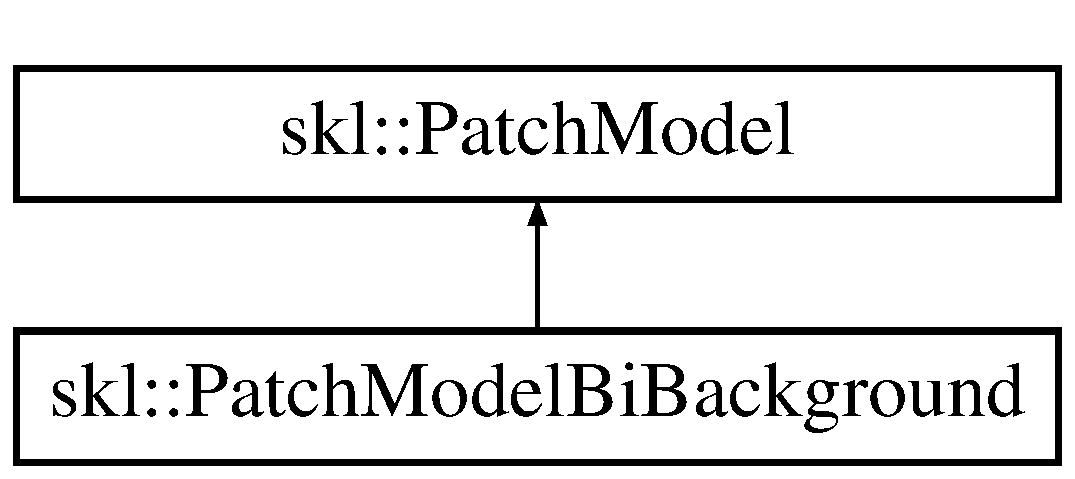
\includegraphics[height=2.000000cm]{classskl_1_1_patch_model}
\end{center}
\end{figure}
\subsection*{Public Member Functions}
\begin{DoxyCompactItemize}
\item 
\hypertarget{classskl_1_1_patch_model_aeac5af0362e5aa9a17b5032cd5787e38}{}\label{classskl_1_1_patch_model_aeac5af0362e5aa9a17b5032cd5787e38} 
{\bfseries Patch\+Model} (const cv\+::\+Mat \&base)
\item 
\hypertarget{classskl_1_1_patch_model_ab7b1f4e65e3fbc4a8d09a0c66bca618c}{}\label{classskl_1_1_patch_model_ab7b1f4e65e3fbc4a8d09a0c66bca618c} 
\hyperlink{classskl_1_1_patch}{Patch} \& {\bfseries operator()} (size\+\_\+t ID)
\item 
\hypertarget{classskl_1_1_patch_model_a044c551eabb11a2ebd1da0b8c85453d4}{}\label{classskl_1_1_patch_model_a044c551eabb11a2ebd1da0b8c85453d4} 
virtual void {\bfseries set\+Object\+Labels} (const cv\+::\+Mat \&img, const cv\+::\+Mat \&human\+\_\+label, const cv\+::\+Mat \&object\+\_\+cand\+\_\+labels, size\+\_\+t object\+\_\+cand\+\_\+num, std\+::vector$<$ size\+\_\+t $>$ $\ast$put\+\_\+object\+\_\+ids, std\+::vector$<$ size\+\_\+t $>$ $\ast$taken\+\_\+object\+\_\+ids)
\item 
\hypertarget{classskl_1_1_patch_model_a8b8e67814d07d164a8001c2d7182159f}{}\label{classskl_1_1_patch_model_a8b8e67814d07d164a8001c2d7182159f} 
void {\bfseries save} (const std\+::string \&file\+\_\+head, const std\+::string \&ext) const
\item 
\hypertarget{classskl_1_1_patch_model_a8dd4f665030782c88e1c43e1791db427}{}\label{classskl_1_1_patch_model_a8dd4f665030782c88e1c43e1791db427} 
const \hyperlink{classskl_1_1_patch}{Patch} \& {\bfseries operator\mbox{[}$\,$\mbox{]}} (size\+\_\+t ID) const
\item 
\hypertarget{classskl_1_1_patch_model_a28fd67d405a7bba59663cfdae1a0a6cb}{}\label{classskl_1_1_patch_model_a28fd67d405a7bba59663cfdae1a0a6cb} 
virtual bool {\bfseries erase} (size\+\_\+t ID)
\item 
\hypertarget{classskl_1_1_patch_model_a92ec1672e24adbb28b9ac30bed4cde59}{}\label{classskl_1_1_patch_model_a92ec1672e24adbb28b9ac30bed4cde59} 
virtual void {\bfseries base} (const cv\+::\+Mat \&\+\_\+\+\_\+bg)
\item 
\hypertarget{classskl_1_1_patch_model_a698cd109a2a2ebc425e62017afcc48ae}{}\label{classskl_1_1_patch_model_a698cd109a2a2ebc425e62017afcc48ae} 
const cv\+::\+Mat \& {\bfseries base} () const
\item 
\hypertarget{classskl_1_1_patch_model_a431184dc94a7f189db4b33d7f7f1d768}{}\label{classskl_1_1_patch_model_a431184dc94a7f189db4b33d7f7f1d768} 
void {\bfseries latest\+\_\+bg} (const cv\+::\+Mat \&bg)
\item 
\hypertarget{classskl_1_1_patch_model_a8264c3659b3ea8ff56024a3e1f308395}{}\label{classskl_1_1_patch_model_a8264c3659b3ea8ff56024a3e1f308395} 
const cv\+::\+Mat \& {\bfseries latest\+\_\+bg} () const
\item 
\hypertarget{classskl_1_1_patch_model_ad11cc2666d1bb775c9c7da34431d3853}{}\label{classskl_1_1_patch_model_ad11cc2666d1bb775c9c7da34431d3853} 
const std\+::list$<$ size\+\_\+t $>$ \& {\bfseries hidden\+\_\+objects} () const
\item 
\hypertarget{classskl_1_1_patch_model_accefbe2067c2c8c29fb5d989709f7be4}{}\label{classskl_1_1_patch_model_accefbe2067c2c8c29fb5d989709f7be4} 
const std\+::list$<$ size\+\_\+t $>$ \& {\bfseries newly\+\_\+hidden\+\_\+objects} () const
\item 
\hypertarget{classskl_1_1_patch_model_ae4bc12f861ba1ad21ef7966771f43d4a}{}\label{classskl_1_1_patch_model_ae4bc12f861ba1ad21ef7966771f43d4a} 
const std\+::list$<$ size\+\_\+t $>$ \& {\bfseries reappeared\+\_\+objects} () const
\item 
\hypertarget{classskl_1_1_patch_model_a9ea1281d94017e968185493bc7551e42}{}\label{classskl_1_1_patch_model_a9ea1281d94017e968185493bc7551e42} 
const cv\+::\+Mat \& {\bfseries updated\+\_\+mask} ()
\item 
\hypertarget{classskl_1_1_patch_model_a60c6fc2c551f5653d54c1ba625653524}{}\label{classskl_1_1_patch_model_a60c6fc2c551f5653d54c1ba625653524} 
void {\bfseries remove\+Patch\+From\+Model} (size\+\_\+t id)
\end{DoxyCompactItemize}
\subsection*{Protected Member Functions}
\begin{DoxyCompactItemize}
\item 
\hypertarget{classskl_1_1_patch_model_ad7905ca278a70e87cceaad2ff2273b6f}{}\label{classskl_1_1_patch_model_ad7905ca278a70e87cceaad2ff2273b6f} 
virtual size\+\_\+t {\bfseries put\+Patch} (const cv\+::\+Mat \&img, const cv\+::\+Mat \&fg\+\_\+edge, const cv\+::\+Mat \&mask, const cv\+::\+Rect \&roi)
\item 
\hypertarget{classskl_1_1_patch_model_a1b4c7a5c43d539c98244bdab51879f59}{}\label{classskl_1_1_patch_model_a1b4c7a5c43d539c98244bdab51879f59} 
virtual void {\bfseries take\+Patch} (size\+\_\+t ID, std\+::vector$<$ size\+\_\+t $>$ $\ast$taken\+\_\+patch\+\_\+ids)
\item 
\hypertarget{classskl_1_1_patch_model_aa0b071c51878060ea7f542279ea9d741}{}\label{classskl_1_1_patch_model_aa0b071c51878060ea7f542279ea9d741} 
void {\bfseries get\+Hidden\+Patches} (const cv\+::\+Mat \&human\+\_\+mask, std\+::list$<$ size\+\_\+t $>$ $\ast$hidden\+\_\+patch\+\_\+ids)
\item 
\hypertarget{classskl_1_1_patch_model_ae461451d928d786f2b1a6859b7acae43}{}\label{classskl_1_1_patch_model_ae461451d928d786f2b1a6859b7acae43} 
bool {\bfseries check\+Taken\+Object} (const \hyperlink{classskl_1_1_patch}{Patch} \&patch, const cv\+::\+Mat \&bg\+\_\+edge, const cv\+::\+Rect $\ast$roi2=N\+U\+LL) const
\item 
\hypertarget{classskl_1_1_patch_model_a78a7921db7d860b04b3d074625070272}{}\label{classskl_1_1_patch_model_a78a7921db7d860b04b3d074625070272} 
size\+\_\+t {\bfseries check\+Taken\+Object} (const cv\+::\+Mat \&bg\+\_\+edge, const cv\+::\+Rect \&roi) const
\item 
\hypertarget{classskl_1_1_patch_model_a72bcc7c60cc145286066eae25428773b}{}\label{classskl_1_1_patch_model_a72bcc7c60cc145286066eae25428773b} 
virtual void {\bfseries update} ()
\item 
\hypertarget{classskl_1_1_patch_model_a52e5eb73c87a149455cecc3f9a0e2a82}{}\label{classskl_1_1_patch_model_a52e5eb73c87a149455cecc3f9a0e2a82} 
void {\bfseries update\+Hidden\+State} (std\+::list$<$ size\+\_\+t $>$ \&\+\_\+\+\_\+hidden\+\_\+object)
\end{DoxyCompactItemize}
\subsection*{Static Protected Member Functions}
\begin{DoxyCompactItemize}
\item 
\hypertarget{classskl_1_1_patch_model_aa6f2a5d23c0402c064a9d31eca29b23f}{}\label{classskl_1_1_patch_model_aa6f2a5d23c0402c064a9d31eca29b23f} 
static double {\bfseries calc\+Common\+Edge} (const Cv\+Rect \&common\+\_\+rect, const \hyperlink{classskl_1_1_patch}{Patch} \&patch\+\_\+1, const \hyperlink{classskl_1_1_patch}{Patch} \&patch\+\_\+2)
\item 
\hypertarget{classskl_1_1_patch_model_a4f0ce6af9380ddd1341cd0b456aa73b1}{}\label{classskl_1_1_patch_model_a4f0ce6af9380ddd1341cd0b456aa73b1} 
static void {\bfseries get\+Object\+Sample\+Points} (const cv\+::\+Mat \&mask, std\+::vector$<$ cv\+::\+Point $>$ $\ast$points)
\end{DoxyCompactItemize}
\subsection*{Protected Attributes}
\begin{DoxyCompactItemize}
\item 
\hypertarget{classskl_1_1_patch_model_abb3d094d92f8d8332c5af2ba19bb08b6}{}\label{classskl_1_1_patch_model_abb3d094d92f8d8332c5af2ba19bb08b6} 
std\+::map$<$ size\+\_\+t, \hyperlink{classskl_1_1_patch}{Patch} $>$ {\bfseries patches}
\item 
\hypertarget{classskl_1_1_patch_model_aa1123ccba2f88ceadae4f527a7050d7e}{}\label{classskl_1_1_patch_model_aa1123ccba2f88ceadae4f527a7050d7e} 
std\+::map$<$ size\+\_\+t, cv\+::\+Mat $>$ {\bfseries patches\+\_\+underside}
\item 
\hypertarget{classskl_1_1_patch_model_a64d22efe5341f9a42b0f970bfd79ab02}{}\label{classskl_1_1_patch_model_a64d22efe5341f9a42b0f970bfd79ab02} 
cv\+::\+Mat {\bfseries \+\_\+latest\+\_\+bg}
\item 
\hypertarget{classskl_1_1_patch_model_a3f03f38a6e96857261840bf725548c04}{}\label{classskl_1_1_patch_model_a3f03f38a6e96857261840bf725548c04} 
cv\+::\+Mat {\bfseries \+\_\+base}
\item 
\hypertarget{classskl_1_1_patch_model_a60cc251b084acf807c48edc5b7d3cd59}{}\label{classskl_1_1_patch_model_a60cc251b084acf807c48edc5b7d3cd59} 
\hyperlink{classskl_1_1_patch_layer}{Patch\+Layer} {\bfseries layer}
\item 
\hypertarget{classskl_1_1_patch_model_aed5671d4a8d8f3e3449c2361ac0acc99}{}\label{classskl_1_1_patch_model_aed5671d4a8d8f3e3449c2361ac0acc99} 
size\+\_\+t {\bfseries max\+\_\+id}
\item 
\hypertarget{classskl_1_1_patch_model_a2e418abf9b17dae7acbfb8efb4439e91}{}\label{classskl_1_1_patch_model_a2e418abf9b17dae7acbfb8efb4439e91} 
std\+::vector$<$ size\+\_\+t $>$ {\bfseries put\+\_\+list}
\item 
\hypertarget{classskl_1_1_patch_model_a29a8acfda73d9cd90dee1e6c198235c0}{}\label{classskl_1_1_patch_model_a29a8acfda73d9cd90dee1e6c198235c0} 
cv\+::\+Mat {\bfseries hidden\+\_\+image}
\item 
\hypertarget{classskl_1_1_patch_model_a0c9e62abe8b48655f6617ce7c689b79f}{}\label{classskl_1_1_patch_model_a0c9e62abe8b48655f6617ce7c689b79f} 
cv\+::\+Mat {\bfseries hidden\+\_\+mask}
\item 
\hypertarget{classskl_1_1_patch_model_a103941995f4263a5b2de173f124d2ae1}{}\label{classskl_1_1_patch_model_a103941995f4263a5b2de173f124d2ae1} 
cv\+::\+Mat {\bfseries \+\_\+updated\+\_\+mask}
\item 
\hypertarget{classskl_1_1_patch_model_a04e87619d969bf0feb95d6cef58aee38}{}\label{classskl_1_1_patch_model_a04e87619d969bf0feb95d6cef58aee38} 
bool {\bfseries changed\+\_\+bg}
\item 
\hypertarget{classskl_1_1_patch_model_ae2d183017afc081074fc6172b801ddff}{}\label{classskl_1_1_patch_model_ae2d183017afc081074fc6172b801ddff} 
bool {\bfseries changed\+\_\+fg}
\item 
\hypertarget{classskl_1_1_patch_model_a685ba43b43d79c6367ffe9756a57ae0c}{}\label{classskl_1_1_patch_model_a685ba43b43d79c6367ffe9756a57ae0c} 
std\+::list$<$ size\+\_\+t $>$ {\bfseries \+\_\+hidden\+\_\+objects}
\item 
\hypertarget{classskl_1_1_patch_model_a5513394f563a573422b212a4b52a3f8d}{}\label{classskl_1_1_patch_model_a5513394f563a573422b212a4b52a3f8d} 
std\+::list$<$ size\+\_\+t $>$ {\bfseries \+\_\+newly\+\_\+hidden\+\_\+objects}
\item 
\hypertarget{classskl_1_1_patch_model_aec19f93cb798d912d0abeea15822d772}{}\label{classskl_1_1_patch_model_aec19f93cb798d912d0abeea15822d772} 
std\+::list$<$ size\+\_\+t $>$ {\bfseries \+\_\+reappeared\+\_\+objects}
\item 
\hypertarget{classskl_1_1_patch_model_a7f89389707a3ccc624cde071f0b97007}{}\label{classskl_1_1_patch_model_a7f89389707a3ccc624cde071f0b97007} 
std\+::vector$<$ bool $>$ {\bfseries on\+\_\+table}
\end{DoxyCompactItemize}
\subsection*{Friends}
\begin{DoxyCompactItemize}
\item 
\hypertarget{classskl_1_1_patch_model_a21c4d8aa35ab6b7ca00f74ceb9c62451}{}\label{classskl_1_1_patch_model_a21c4d8aa35ab6b7ca00f74ceb9c62451} 
class {\bfseries Patch\+Layer}
\item 
\hypertarget{classskl_1_1_patch_model_a06137dac0e3c805556caa28e75365d9f}{}\label{classskl_1_1_patch_model_a06137dac0e3c805556caa28e75365d9f} 
class {\bfseries Patch\+Tracker}
\end{DoxyCompactItemize}


The documentation for this class was generated from the following files\+:\begin{DoxyCompactItemize}
\item 
Open\+C\+V/include/\hyperlink{_patch_model_8h}{Patch\+Model.\+h}\item 
Open\+C\+V/src/\hyperlink{_patch_model_8cpp}{Patch\+Model.\+cpp}\end{DoxyCompactItemize}

\hypertarget{classskl_1_1_patch_model_bi_background}{}\section{skl\+:\+:Patch\+Model\+Bi\+Background Class Reference}
\label{classskl_1_1_patch_model_bi_background}\index{skl\+::\+Patch\+Model\+Bi\+Background@{skl\+::\+Patch\+Model\+Bi\+Background}}


複数の背景を持つパッチモデル  




{\ttfamily \#include $<$Patch\+Model\+Bi\+Background.\+h$>$}

Inheritance diagram for skl\+:\+:Patch\+Model\+Bi\+Background\+:\begin{figure}[H]
\begin{center}
\leavevmode
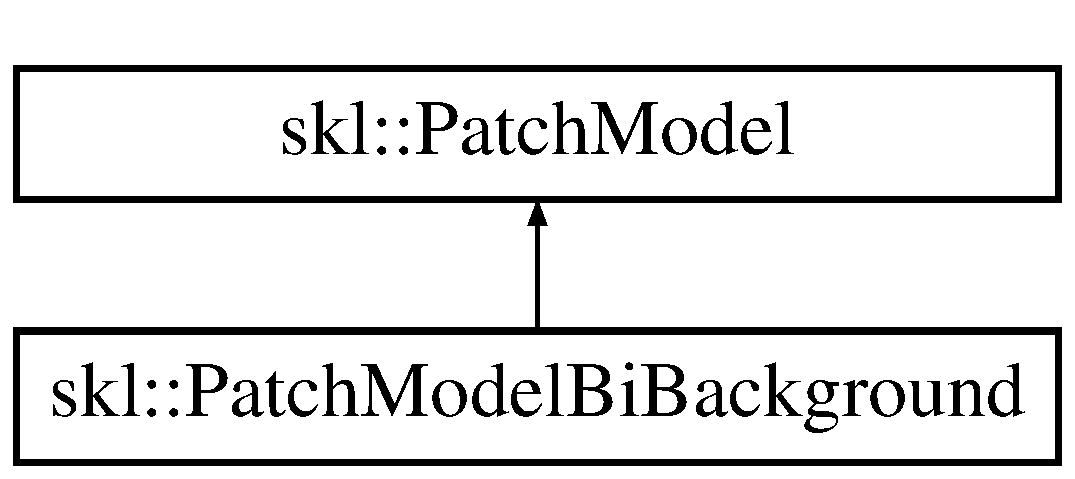
\includegraphics[height=2.000000cm]{classskl_1_1_patch_model_bi_background}
\end{center}
\end{figure}
\subsection*{Public Member Functions}
\begin{DoxyCompactItemize}
\item 
\hypertarget{classskl_1_1_patch_model_bi_background_ad3813e93a67f1f3921f4dc116ac0f8d4}{}\label{classskl_1_1_patch_model_bi_background_ad3813e93a67f1f3921f4dc116ac0f8d4} 
\hyperlink{classskl_1_1_patch_model_bi_background_ad3813e93a67f1f3921f4dc116ac0f8d4}{Patch\+Model\+Bi\+Background} ()
\begin{DoxyCompactList}\small\item\em デフォルトコンストラクタ \end{DoxyCompactList}\item 
\hypertarget{classskl_1_1_patch_model_bi_background_aeb304f991c2e68c0628b046fa9d8e091}{}\label{classskl_1_1_patch_model_bi_background_aeb304f991c2e68c0628b046fa9d8e091} 
\hyperlink{classskl_1_1_patch_model_bi_background_aeb304f991c2e68c0628b046fa9d8e091}{Patch\+Model\+Bi\+Background} (const cv\+::\+Mat \&base)
\begin{DoxyCompactList}\small\item\em 背景画像を引数に取るコンストラクタ \end{DoxyCompactList}\item 
\hypertarget{classskl_1_1_patch_model_bi_background_a223018a69ee36da60092cc9e2b9ea6ca}{}\label{classskl_1_1_patch_model_bi_background_a223018a69ee36da60092cc9e2b9ea6ca} 
virtual \hyperlink{classskl_1_1_patch_model_bi_background_a223018a69ee36da60092cc9e2b9ea6ca}{$\sim$\+Patch\+Model\+Bi\+Background} ()
\begin{DoxyCompactList}\small\item\em デストラクタ \end{DoxyCompactList}\item 
\hypertarget{classskl_1_1_patch_model_bi_background_aa720b6806d9742ef75fef2f905ec9396}{}\label{classskl_1_1_patch_model_bi_background_aa720b6806d9742ef75fef2f905ec9396} 
void {\bfseries set\+Object\+Labels} (const cv\+::\+Mat \&img, const cv\+::\+Mat \&human\+\_\+label, const cv\+::\+Mat \&object\+\_\+cand\+\_\+labels, size\+\_\+t object\+\_\+cand\+\_\+num, std\+::vector$<$ size\+\_\+t $>$ $\ast$put\+\_\+object\+\_\+ids, std\+::vector$<$ size\+\_\+t $>$ $\ast$taken\+\_\+object\+\_\+ids)
\item 
\hypertarget{classskl_1_1_patch_model_bi_background_a65303d6831841eb507c2b9556e553a43}{}\label{classskl_1_1_patch_model_bi_background_a65303d6831841eb507c2b9556e553a43} 
void {\bfseries remove\+Patch\+From\+Model} (size\+\_\+t id)
\item 
\hypertarget{classskl_1_1_patch_model_bi_background_a062a4ddd81d43392be272dabffd891b5}{}\label{classskl_1_1_patch_model_bi_background_a062a4ddd81d43392be272dabffd891b5} 
void {\bfseries base} (const cv\+::\+Mat \&base\+\_\+bg)
\item 
\hypertarget{classskl_1_1_patch_model_bi_background_a7076aea8f4cdbf1b841b01e07734e9f6}{}\label{classskl_1_1_patch_model_bi_background_a7076aea8f4cdbf1b841b01e07734e9f6} 
void {\bfseries latest\+\_\+bg2} (const cv\+::\+Mat \&bg)
\item 
\hypertarget{classskl_1_1_patch_model_bi_background_a003aba462dc25be800fd6a610015bbf2}{}\label{classskl_1_1_patch_model_bi_background_a003aba462dc25be800fd6a610015bbf2} 
const cv\+::\+Mat \& {\bfseries latest\+\_\+bg2} () const
\item 
\hypertarget{classskl_1_1_patch_model_bi_background_a5d1804b0aa78e775b67ca9df8c0b64a0}{}\label{classskl_1_1_patch_model_bi_background_a5d1804b0aa78e775b67ca9df8c0b64a0} 
bool {\bfseries erase} (size\+\_\+t ID)
\end{DoxyCompactItemize}
\subsection*{Protected Member Functions}
\begin{DoxyCompactItemize}
\item 
\hypertarget{classskl_1_1_patch_model_bi_background_a8cc32d4d6f0ccd12f51c2eb43f56f615}{}\label{classskl_1_1_patch_model_bi_background_a8cc32d4d6f0ccd12f51c2eb43f56f615} 
virtual size\+\_\+t {\bfseries put\+Patch} (const cv\+::\+Mat \&img, const cv\+::\+Mat \&fg\+\_\+edge, const cv\+::\+Mat \&mask, const cv\+::\+Rect \&roi)
\item 
\hypertarget{classskl_1_1_patch_model_bi_background_ad1aefd40d2fb6f7ccd540f9cbd512118}{}\label{classskl_1_1_patch_model_bi_background_ad1aefd40d2fb6f7ccd540f9cbd512118} 
virtual void {\bfseries take\+Patch} (size\+\_\+t ID, std\+::vector$<$ size\+\_\+t $>$ $\ast$taken\+\_\+patch\+\_\+ids)
\item 
\hypertarget{classskl_1_1_patch_model_bi_background_ac491c5b0cd10591ee0ac7a2e4a3108ea}{}\label{classskl_1_1_patch_model_bi_background_ac491c5b0cd10591ee0ac7a2e4a3108ea} 
virtual void {\bfseries update} ()
\end{DoxyCompactItemize}
\subsection*{Protected Attributes}
\begin{DoxyCompactItemize}
\item 
\hypertarget{classskl_1_1_patch_model_bi_background_acd9abc34b8445307c31e731094f1bf74}{}\label{classskl_1_1_patch_model_bi_background_acd9abc34b8445307c31e731094f1bf74} 
std\+::map$<$ size\+\_\+t, cv\+::\+Mat $>$ {\bfseries patches\+\_\+underside2}
\item 
\hypertarget{classskl_1_1_patch_model_bi_background_a599460502cd7df137d5c1e14a2798d13}{}\label{classskl_1_1_patch_model_bi_background_a599460502cd7df137d5c1e14a2798d13} 
cv\+::\+Mat {\bfseries \+\_\+latest\+\_\+bg2}
\item 
\hypertarget{classskl_1_1_patch_model_bi_background_abfe3ac42763123a21443d640f9f0cc1d}{}\label{classskl_1_1_patch_model_bi_background_abfe3ac42763123a21443d640f9f0cc1d} 
cv\+::\+Mat {\bfseries hidden\+\_\+image2}
\end{DoxyCompactItemize}
\subsection*{Additional Inherited Members}


\subsection{Detailed Description}
複数の背景を持つパッチモデル 

The documentation for this class was generated from the following files\+:\begin{DoxyCompactItemize}
\item 
Open\+C\+V/include/\hyperlink{_patch_model_bi_background_8h}{Patch\+Model\+Bi\+Background.\+h}\item 
Open\+C\+V/src/\hyperlink{_patch_model_bi_background_8cpp}{Patch\+Model\+Bi\+Background.\+cpp}\end{DoxyCompactItemize}

\hypertarget{classskl_1_1_printable}{}\section{skl\+:\+:Printable$<$ T $>$ Class Template Reference}
\label{classskl_1_1_printable}\index{skl\+::\+Printable$<$ T $>$@{skl\+::\+Printable$<$ T $>$}}


文字列として書き出しが可能であることを保証するインターフェイス  




{\ttfamily \#include $<$Printable.\+h$>$}

Inheritance diagram for skl\+:\+:Printable$<$ T $>$\+:\begin{figure}[H]
\begin{center}
\leavevmode
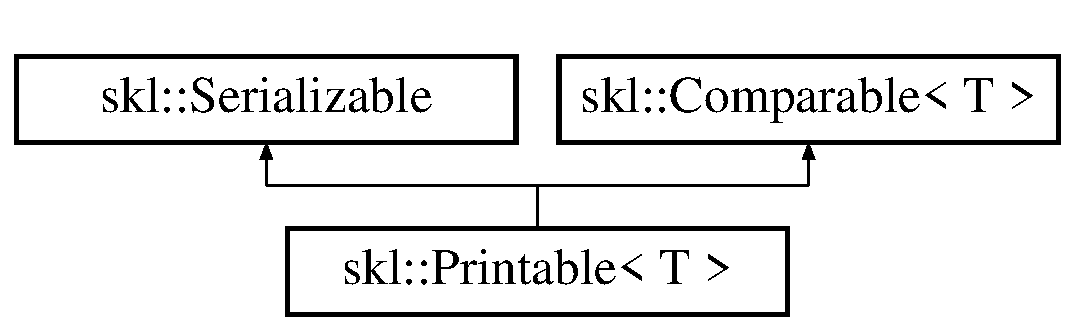
\includegraphics[height=2.000000cm]{classskl_1_1_printable}
\end{center}
\end{figure}
\subsection*{Public Member Functions}
\begin{DoxyCompactItemize}
\item 
\hypertarget{classskl_1_1_printable_ab1d9cf680b6431052ca4692aaef1f106}{}\label{classskl_1_1_printable_ab1d9cf680b6431052ca4692aaef1f106} 
\hyperlink{classskl_1_1_printable_ab1d9cf680b6431052ca4692aaef1f106}{Printable} ()
\begin{DoxyCompactList}\small\item\em デフォルトコンストラクタ \end{DoxyCompactList}\item 
\hypertarget{classskl_1_1_printable_ad299a8e5955a80154aa656d178a9992e}{}\label{classskl_1_1_printable_ad299a8e5955a80154aa656d178a9992e} 
virtual \hyperlink{classskl_1_1_printable_ad299a8e5955a80154aa656d178a9992e}{$\sim$\+Printable} ()
\begin{DoxyCompactList}\small\item\em デストラクタ \end{DoxyCompactList}\item 
\hypertarget{classskl_1_1_printable_ad27d5ef1bb67b50e89db983d106cc9d1}{}\label{classskl_1_1_printable_ad27d5ef1bb67b50e89db983d106cc9d1} 
virtual std\+::string {\bfseries print} () const =0
\item 
\hypertarget{classskl_1_1_printable_a7f99b93dcf3250ac0861f2660103f8a8}{}\label{classskl_1_1_printable_a7f99b93dcf3250ac0861f2660103f8a8} 
virtual bool {\bfseries scan} (const std\+::string \&str)=0
\item 
\hypertarget{classskl_1_1_printable_a72ab64dc61dbecebef3211b72814f978}{}\label{classskl_1_1_printable_a72ab64dc61dbecebef3211b72814f978} 
virtual \hyperlink{classskl_1_1_printable}{Printable}$<$ T $>$ \& \hyperlink{classskl_1_1_printable_a72ab64dc61dbecebef3211b72814f978}{operator=} (const \hyperlink{classskl_1_1_printable}{Printable}$<$ T $>$ \&other)
\begin{DoxyCompactList}\small\item\em 代入演算子 \end{DoxyCompactList}\item 
\hypertarget{classskl_1_1_printable_a57ee1e53f47772b771f41e1b23ee5b82}{}\label{classskl_1_1_printable_a57ee1e53f47772b771f41e1b23ee5b82} 
virtual bool \hyperlink{classskl_1_1_printable_a57ee1e53f47772b771f41e1b23ee5b82}{operator$<$} (const T \&other) const
\begin{DoxyCompactList}\small\item\em 比較演算子(但し、printした文字列の順序を利用するので、意味のある比較をした場合には具象クラス毎に定義すること) \end{DoxyCompactList}\item 
T $\ast$ \hyperlink{classskl_1_1_printable_a1bc18e234d25c4bdce84ed70a58d2f88}{clone} () const
\begin{DoxyCompactList}\small\item\em cloneを作る \end{DoxyCompactList}\end{DoxyCompactItemize}
\subsection*{Protected Member Functions}
\begin{DoxyCompactItemize}
\item 
\hypertarget{classskl_1_1_printable_a79a8c40232c97197722b0e50c3bc3ccf}{}\label{classskl_1_1_printable_a79a8c40232c97197722b0e50c3bc3ccf} 
virtual long \hyperlink{classskl_1_1_printable_a79a8c40232c97197722b0e50c3bc3ccf}{\+\_\+buf\+\_\+size} () const
\begin{DoxyCompactList}\small\item\em \+\_\+serializeで生成される予定のbufの長さを返す \end{DoxyCompactList}\item 
\hypertarget{classskl_1_1_printable_ab7ee46a0d3fd3536af70929e477eefd4}{}\label{classskl_1_1_printable_ab7ee46a0d3fd3536af70929e477eefd4} 
virtual void \hyperlink{classskl_1_1_printable_ab7ee46a0d3fd3536af70929e477eefd4}{\+\_\+serialize} ()
\begin{DoxyCompactList}\small\item\em クラスの中身を直列化してメンバ変数のbufに格納する \end{DoxyCompactList}\item 
\hypertarget{classskl_1_1_printable_a1f05fcd22b8e76f3e2da7d60f31afb58}{}\label{classskl_1_1_printable_a1f05fcd22b8e76f3e2da7d60f31afb58} 
virtual void \hyperlink{classskl_1_1_printable_a1f05fcd22b8e76f3e2da7d60f31afb58}{\+\_\+deserialize} (const char $\ast$\hyperlink{classskl_1_1_serializable_a1d203d9f0049ce37183a0dcefbc6399a}{buf}, long \hyperlink{classskl_1_1_serializable_a087eb19fada917a42b8411bfecbac0f1}{buf\+\_\+size})
\begin{DoxyCompactList}\small\item\em 直列化されたクラスの中身を読み込む \end{DoxyCompactList}\end{DoxyCompactItemize}
\subsection*{Additional Inherited Members}


\subsection{Detailed Description}
\subsubsection*{template$<$class T$>$\newline
class skl\+::\+Printable$<$ T $>$}

文字列として書き出しが可能であることを保証するインターフェイス 

\subsection{Member Function Documentation}
\hypertarget{classskl_1_1_printable_a1bc18e234d25c4bdce84ed70a58d2f88}{}\label{classskl_1_1_printable_a1bc18e234d25c4bdce84ed70a58d2f88} 
\index{skl\+::\+Printable@{skl\+::\+Printable}!clone@{clone}}
\index{clone@{clone}!skl\+::\+Printable@{skl\+::\+Printable}}
\subsubsection{\texorpdfstring{clone()}{clone()}}
{\footnotesize\ttfamily template$<$class T $>$ \\
T $\ast$ \hyperlink{classskl_1_1_printable}{skl\+::\+Printable}$<$ T $>$\+::clone (\begin{DoxyParamCaption}{ }\end{DoxyParamCaption}) const}



cloneを作る 

\begin{DoxyReturn}{Returns}
新しく作られたインスタンス 
\end{DoxyReturn}


The documentation for this class was generated from the following file\+:\begin{DoxyCompactItemize}
\item 
Core/include/\hyperlink{_printable_8h}{Printable.\+h}\end{DoxyCompactItemize}

\hypertarget{class_labeling_1_1_raster_segment}{}\section{Labeling$<$ SrcT, DstT $>$\+:\+:Raster\+Segment Class Reference}
\label{class_labeling_1_1_raster_segment}\index{Labeling$<$ Src\+T, Dst\+T $>$\+::\+Raster\+Segment@{Labeling$<$ Src\+T, Dst\+T $>$\+::\+Raster\+Segment}}


\hyperlink{class_labeling_1_1_raster_segment}{Raster\+Segment}.  




{\ttfamily \#include $<$Labeling.\+h$>$}

\subsection*{Public Member Functions}
\begin{DoxyCompactItemize}
\item 
\hypertarget{class_labeling_1_1_raster_segment_a038378c28d61700aba53dc77d166ff1b}{}\label{class_labeling_1_1_raster_segment_a038378c28d61700aba53dc77d166ff1b} 
{\bfseries Raster\+Segment} (const int n\+\_\+left\+\_\+x, const int n\+\_\+right\+\_\+x, const int n\+\_\+y, const SrcT n\+\_\+source\+\_\+value)
\item 
\hypertarget{class_labeling_1_1_raster_segment_a1a15635f3be37d578dd97d58fd6f0693}{}\label{class_labeling_1_1_raster_segment_a1a15635f3be37d578dd97d58fd6f0693} 
int {\bfseries Get\+LeftX} (void) const
\item 
\hypertarget{class_labeling_1_1_raster_segment_a0c71ece8e7bf6976303de878e4b649e6}{}\label{class_labeling_1_1_raster_segment_a0c71ece8e7bf6976303de878e4b649e6} 
int {\bfseries Get\+RightX} (void) const
\item 
\hypertarget{class_labeling_1_1_raster_segment_ab2012942902b1c773af763d03745c81c}{}\label{class_labeling_1_1_raster_segment_ab2012942902b1c773af763d03745c81c} 
int {\bfseries GetY} (void) const
\item 
\hypertarget{class_labeling_1_1_raster_segment_a61ea6bd9568ad291c4ab82f74e7c3df4}{}\label{class_labeling_1_1_raster_segment_a61ea6bd9568ad291c4ab82f74e7c3df4} 
SrcT {\bfseries Get\+Source\+Value} (void) const
\item 
\hypertarget{class_labeling_1_1_raster_segment_af1ab96570b660c4100703977f7b4d3c4}{}\label{class_labeling_1_1_raster_segment_af1ab96570b660c4100703977f7b4d3c4} 
int {\bfseries LeftX} (void) const
\item 
\hypertarget{class_labeling_1_1_raster_segment_a885de7fccb6ab86adb7715eaeeb205d0}{}\label{class_labeling_1_1_raster_segment_a885de7fccb6ab86adb7715eaeeb205d0} 
int {\bfseries RightX} (void) const
\item 
\hypertarget{class_labeling_1_1_raster_segment_a023e28bb05044fc1233ab017e0565897}{}\label{class_labeling_1_1_raster_segment_a023e28bb05044fc1233ab017e0565897} 
int {\bfseries Y} (void) const
\item 
\hypertarget{class_labeling_1_1_raster_segment_aea069bf94270bff59334d4645f37966e}{}\label{class_labeling_1_1_raster_segment_aea069bf94270bff59334d4645f37966e} 
SrcT {\bfseries Source\+Value} (void) const
\end{DoxyCompactItemize}
\subsection*{Friends}
\begin{DoxyCompactItemize}
\item 
\hypertarget{class_labeling_1_1_raster_segment_ad69e5ef7abb3c0a38b8d66e137e05e79}{}\label{class_labeling_1_1_raster_segment_ad69e5ef7abb3c0a38b8d66e137e05e79} 
std\+::ostream \& {\bfseries operator$<$$<$} (std\+::ostream \&s, \hyperlink{class_labeling_1_1_raster_segment}{Raster\+Segment} \&rs)
\end{DoxyCompactItemize}


\subsection{Detailed Description}
\subsubsection*{template$<$class SrcT, class DstT$>$\newline
class Labeling$<$ Src\+T, Dst\+T $>$\+::\+Raster\+Segment}

\hyperlink{class_labeling_1_1_raster_segment}{Raster\+Segment}. 

ラベリングを行うクラス。 

The documentation for this class was generated from the following file\+:\begin{DoxyCompactItemize}
\item 
Open\+C\+V/include/\hyperlink{_labeling_8h}{Labeling.\+h}\end{DoxyCompactItemize}

\hypertarget{class_labeling_1_1_region_info}{}\section{Labeling$<$ SrcT, DstT $>$\+:\+:Region\+Info Class Reference}
\label{class_labeling_1_1_region_info}\index{Labeling$<$ Src\+T, Dst\+T $>$\+::\+Region\+Info@{Labeling$<$ Src\+T, Dst\+T $>$\+::\+Region\+Info}}
\subsection*{Public Member Functions}
\begin{DoxyCompactItemize}
\item 
\hypertarget{class_labeling_1_1_region_info_a628e08b513def13ce73f6bdbb2ad49cc}{}\label{class_labeling_1_1_region_info_a628e08b513def13ce73f6bdbb2ad49cc} 
void {\bfseries Set\+Num\+Of\+Pixels} (const int n\+\_\+num\+\_\+of\+\_\+pixels)
\item 
\hypertarget{class_labeling_1_1_region_info_a18233b64cd08822e6ed2eb5d2541178c}{}\label{class_labeling_1_1_region_info_a18233b64cd08822e6ed2eb5d2541178c} 
void {\bfseries Set\+Center} (const float x, const float y)
\item 
\hypertarget{class_labeling_1_1_region_info_a60a72592f3177344c7f35a5ce6f9ea51}{}\label{class_labeling_1_1_region_info_a60a72592f3177344c7f35a5ce6f9ea51} 
void {\bfseries Set\+Size} (const int x, const int y)
\item 
\hypertarget{class_labeling_1_1_region_info_a4e515a1846f9ff44f564c1e062122b78}{}\label{class_labeling_1_1_region_info_a4e515a1846f9ff44f564c1e062122b78} 
void {\bfseries Set\+Min} (const int x, const int y)
\item 
\hypertarget{class_labeling_1_1_region_info_a8a3d7201cab55adeb47d1da201d4206d}{}\label{class_labeling_1_1_region_info_a8a3d7201cab55adeb47d1da201d4206d} 
void {\bfseries Set\+Max} (const int x, const int y)
\item 
\hypertarget{class_labeling_1_1_region_info_aa16d4a02f4ca759d654a81e96b9a02c1}{}\label{class_labeling_1_1_region_info_aa16d4a02f4ca759d654a81e96b9a02c1} 
void {\bfseries Set\+Min\+Max} (const int n\+\_\+min\+\_\+x, const int n\+\_\+min\+\_\+y, const int n\+\_\+max\+\_\+x, const int n\+\_\+max\+\_\+y)
\item 
\hypertarget{class_labeling_1_1_region_info_a517b8b2b94aa9d0e19cb216114f66463}{}\label{class_labeling_1_1_region_info_a517b8b2b94aa9d0e19cb216114f66463} 
void {\bfseries Set\+Center\+Of\+Gravity} (const float x, const float y)
\item 
\hypertarget{class_labeling_1_1_region_info_a0201a75e76be943592bca8cd356043fb}{}\label{class_labeling_1_1_region_info_a0201a75e76be943592bca8cd356043fb} 
void {\bfseries Set\+Source\+Value} (const SrcT n\+\_\+source\+\_\+value)
\item 
\hypertarget{class_labeling_1_1_region_info_ac97c903d9e3eb9f77be6ccf9ccdbf2c0}{}\label{class_labeling_1_1_region_info_ac97c903d9e3eb9f77be6ccf9ccdbf2c0} 
void {\bfseries Set\+Result} (const DstT n\+\_\+result)
\item 
\hypertarget{class_labeling_1_1_region_info_ae9014e00d562affb3db5c52729db22ce}{}\label{class_labeling_1_1_region_info_ae9014e00d562affb3db5c52729db22ce} 
int {\bfseries Get\+Num\+Of\+Pixels} (void) const
\item 
\hypertarget{class_labeling_1_1_region_info_a2eea6ea04e7b40dfcefd1605040a018c}{}\label{class_labeling_1_1_region_info_a2eea6ea04e7b40dfcefd1605040a018c} 
void {\bfseries Get\+Center} (float \&x, float \&y) const
\item 
\hypertarget{class_labeling_1_1_region_info_adc840bde00b274ce0cedb98083b87df8}{}\label{class_labeling_1_1_region_info_adc840bde00b274ce0cedb98083b87df8} 
void {\bfseries Get\+Size} (int \&x, int \&y) const
\item 
\hypertarget{class_labeling_1_1_region_info_afb5900bfcbd2e4dc40d893c26cd62255}{}\label{class_labeling_1_1_region_info_afb5900bfcbd2e4dc40d893c26cd62255} 
void {\bfseries Get\+Min} (int \&x, int \&y) const
\item 
\hypertarget{class_labeling_1_1_region_info_ac0b0f50f35f5f4477e39bf119ea8716d}{}\label{class_labeling_1_1_region_info_ac0b0f50f35f5f4477e39bf119ea8716d} 
void {\bfseries Get\+Max} (int \&x, int \&y) const
\item 
\hypertarget{class_labeling_1_1_region_info_ab09260d5fb64457dcdcbdc2d34ca486c}{}\label{class_labeling_1_1_region_info_ab09260d5fb64457dcdcbdc2d34ca486c} 
void {\bfseries Get\+Center\+Of\+Gravity} (float \&x, float \&y) const
\item 
\hypertarget{class_labeling_1_1_region_info_a4279075549a1af1df8660fe3b5c4fae5}{}\label{class_labeling_1_1_region_info_a4279075549a1af1df8660fe3b5c4fae5} 
SrcT {\bfseries Get\+Source\+Value} (void) const
\item 
\hypertarget{class_labeling_1_1_region_info_adca2a69f45b33dd2f3f67a17ca17a07b}{}\label{class_labeling_1_1_region_info_adca2a69f45b33dd2f3f67a17ca17a07b} 
DstT {\bfseries Get\+Result} (void) const
\item 
\hypertarget{class_labeling_1_1_region_info_a1a147ca5752a2ac5daebb927ebe49c63}{}\label{class_labeling_1_1_region_info_a1a147ca5752a2ac5daebb927ebe49c63} 
R\+S\+P\+List \& {\bfseries Get\+Raster\+Segment\+List} (void)
\item 
\hypertarget{class_labeling_1_1_region_info_a043096f6f6a64c287307f72f574844ad}{}\label{class_labeling_1_1_region_info_a043096f6f6a64c287307f72f574844ad} 
void {\bfseries Push} (\hyperlink{class_labeling_1_1_raster_segment}{Raster\+Segment} $\ast$rs)
\item 
\hypertarget{class_labeling_1_1_region_info_a7532df61107650edc4ff82b7c2345bd6}{}\label{class_labeling_1_1_region_info_a7532df61107650edc4ff82b7c2345bd6} 
void {\bfseries Pop} (\hyperlink{class_labeling_1_1_raster_segment}{Raster\+Segment} $\ast$\&rs)
\item 
\hypertarget{class_labeling_1_1_region_info_a35eab6cbcd72a73ee7f63e90ffe44f3b}{}\label{class_labeling_1_1_region_info_a35eab6cbcd72a73ee7f63e90ffe44f3b} 
int {\bfseries Get\+Num\+Of\+Raster\+Segments} (void)
\end{DoxyCompactItemize}
\subsection*{Friends}
\begin{DoxyCompactItemize}
\item 
\hypertarget{class_labeling_1_1_region_info_a84e3a082347e41fbcf4a870a9f8f1064}{}\label{class_labeling_1_1_region_info_a84e3a082347e41fbcf4a870a9f8f1064} 
bool {\bfseries operator$<$} (const \hyperlink{class_labeling_1_1_region_info}{Region\+Info} \&l, const \hyperlink{class_labeling_1_1_region_info}{Region\+Info} \&r)
\item 
\hypertarget{class_labeling_1_1_region_info_acf144f688f407a3bcc597cdf22f40c77}{}\label{class_labeling_1_1_region_info_acf144f688f407a3bcc597cdf22f40c77} 
std\+::ostream \& {\bfseries operator$<$$<$} (std\+::ostream \&s, \hyperlink{class_labeling_1_1_region_info}{Region\+Info} \&ri)
\end{DoxyCompactItemize}


The documentation for this class was generated from the following file\+:\begin{DoxyCompactItemize}
\item 
Open\+C\+V/include/\hyperlink{_labeling_8h}{Labeling.\+h}\end{DoxyCompactItemize}

\hypertarget{classskl_1_1_region_labeling_simple}{}\section{skl\+:\+:Region\+Labeling\+Simple Class Reference}
\label{classskl_1_1_region_labeling_simple}\index{skl\+::\+Region\+Labeling\+Simple@{skl\+::\+Region\+Labeling\+Simple}}
Inheritance diagram for skl\+:\+:Region\+Labeling\+Simple\+:\begin{figure}[H]
\begin{center}
\leavevmode
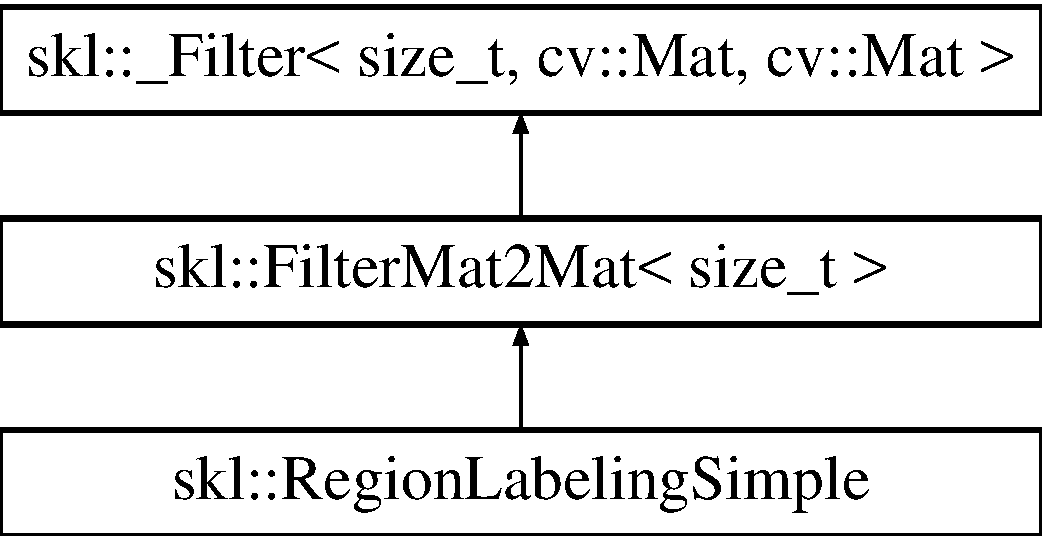
\includegraphics[height=3.000000cm]{classskl_1_1_region_labeling_simple}
\end{center}
\end{figure}
\subsection*{Public Member Functions}
\begin{DoxyCompactItemize}
\item 
\hypertarget{classskl_1_1_region_labeling_simple_acb6a8ecc08c516e774eff602f9eda806}{}\label{classskl_1_1_region_labeling_simple_acb6a8ecc08c516e774eff602f9eda806} 
\hyperlink{classskl_1_1_region_labeling_simple_acb6a8ecc08c516e774eff602f9eda806}{Region\+Labeling\+Simple} (int threshold=30)
\begin{DoxyCompactList}\small\item\em 奈良先端大、井村先生のプログラム(激速)を利用したラベリング 背景色は(0,0,0)でないといけない \end{DoxyCompactList}\item 
\hypertarget{classskl_1_1_region_labeling_simple_a82849b764bb0a8b40dd7c863064d3b59}{}\label{classskl_1_1_region_labeling_simple_a82849b764bb0a8b40dd7c863064d3b59} 
void {\bfseries set\+Threshold} (int threshold)
\item 
\hypertarget{classskl_1_1_region_labeling_simple_a5e35c77b35dbb689aaf0d35fe3c49415}{}\label{classskl_1_1_region_labeling_simple_a5e35c77b35dbb689aaf0d35fe3c49415} 
size\+\_\+t {\bfseries compute} (const cv\+::\+Mat \&img, const cv\+::\+Mat \&mask, cv\+::\+Mat \&labels)
\end{DoxyCompactItemize}
\subsection*{Protected Attributes}
\begin{DoxyCompactItemize}
\item 
\hypertarget{classskl_1_1_region_labeling_simple_ad169a11ec06edf1e100fb4df948b2aca}{}\label{classskl_1_1_region_labeling_simple_ad169a11ec06edf1e100fb4df948b2aca} 
int {\bfseries threshold}
\item 
\hypertarget{classskl_1_1_region_labeling_simple_ad8f7567dc7b8d87ceda74b68c0686ce2}{}\label{classskl_1_1_region_labeling_simple_ad8f7567dc7b8d87ceda74b68c0686ce2} 
\hyperlink{class_labeling}{Labeling\+BS} {\bfseries labeling}
\end{DoxyCompactItemize}


The documentation for this class was generated from the following files\+:\begin{DoxyCompactItemize}
\item 
Open\+C\+V/include/Region\+Labeling\+Simple.\+h\item 
Open\+C\+V/src/Region\+Labeling\+Simple.\+cpp\end{DoxyCompactItemize}

\hypertarget{classskl_1_1_sample_set_reader}{}\section{skl\+:\+:Sample\+Set\+Reader Class Reference}
\label{classskl_1_1_sample_set_reader}\index{skl\+::\+Sample\+Set\+Reader@{skl\+::\+Sample\+Set\+Reader}}


学習用/評価用の特徴量サンプルセットの読み込みを行う  




{\ttfamily \#include $<$Sample\+Set\+Reader.\+h$>$}

\subsection*{Public Member Functions}
\begin{DoxyCompactItemize}
\item 
\hypertarget{classskl_1_1_sample_set_reader_ad10ad73e03fc3ee176ec9d4ab036f45d}{}\label{classskl_1_1_sample_set_reader_ad10ad73e03fc3ee176ec9d4ab036f45d} 
\hyperlink{classskl_1_1_sample_set_reader_ad10ad73e03fc3ee176ec9d4ab036f45d}{Sample\+Set\+Reader} ()
\begin{DoxyCompactList}\small\item\em デフォルトコンストラクタ \end{DoxyCompactList}\item 
\hypertarget{classskl_1_1_sample_set_reader_ae051e482f383da2027f079caf4802127}{}\label{classskl_1_1_sample_set_reader_ae051e482f383da2027f079caf4802127} 
virtual \hyperlink{classskl_1_1_sample_set_reader_ae051e482f383da2027f079caf4802127}{$\sim$\+Sample\+Set\+Reader} ()
\begin{DoxyCompactList}\small\item\em デストラクタ \end{DoxyCompactList}\end{DoxyCompactItemize}
\subsection*{Static Public Member Functions}
\begin{DoxyCompactItemize}
\item 
\hypertarget{classskl_1_1_sample_set_reader_af7e8e42693c480317893320efe1a97bf}{}\label{classskl_1_1_sample_set_reader_af7e8e42693c480317893320efe1a97bf} 
static bool {\bfseries read} (const std\+::string \&filename, cv\+::\+Mat $\ast$samples=N\+U\+LL, cv\+::\+Mat $\ast$responces=N\+U\+LL, cv\+::\+Mat $\ast$likelihoods=N\+U\+LL, std\+::vector$<$ \hyperlink{classskl_1_1_time}{skl\+::\+Time} $>$ $\ast$timestamps=N\+U\+LL, std\+::vector$<$ cv\+::\+Key\+Point $>$ $\ast$keypoints=N\+U\+LL)
\item 
\hypertarget{classskl_1_1_sample_set_reader_aed41b06745e807114ee61b93d9ffbb84}{}\label{classskl_1_1_sample_set_reader_aed41b06745e807114ee61b93d9ffbb84} 
static bool {\bfseries read} (std\+::istream \&in, cv\+::\+Mat $\ast$samples=N\+U\+LL, cv\+::\+Mat $\ast$responces=N\+U\+LL, cv\+::\+Mat $\ast$likelihoods=N\+U\+LL, std\+::vector$<$ \hyperlink{classskl_1_1_time}{skl\+::\+Time} $>$ $\ast$timestamps=N\+U\+LL, std\+::vector$<$ cv\+::\+Key\+Point $>$ $\ast$keypoints=N\+U\+LL)
\end{DoxyCompactItemize}
\subsection*{Static Protected Member Functions}
\begin{DoxyCompactItemize}
\item 
\hypertarget{classskl_1_1_sample_set_reader_ad0a976a1c6ef2958d4a67b4170b5beb4}{}\label{classskl_1_1_sample_set_reader_ad0a976a1c6ef2958d4a67b4170b5beb4} 
static bool {\bfseries skip} (std\+::istream \&in, size\+\_\+t num)
\item 
\hypertarget{classskl_1_1_sample_set_reader_a4a074f7194e0f824741d412e0afeb8a9}{}\label{classskl_1_1_sample_set_reader_a4a074f7194e0f824741d412e0afeb8a9} 
{\footnotesize template$<$class Type , size\+\_\+t C\+V\+\_\+\+D\+E\+P\+TH$>$ }\\static bool {\bfseries \+\_\+read\+Matrix} (std\+::istream \&in, size\+\_\+t cols, size\+\_\+t rows, cv\+::\+Mat \&dist)
\item 
\hypertarget{classskl_1_1_sample_set_reader_ae3fc1347c59fde0c745df2556b14dea0}{}\label{classskl_1_1_sample_set_reader_ae3fc1347c59fde0c745df2556b14dea0} 
static bool {\bfseries \+\_\+read\+Header} (std\+::istream \&in, size\+\_\+t \&sample\+\_\+num, size\+\_\+t \&sample\+\_\+dim, bool \&has\+\_\+responce, size\+\_\+t \&class\+\_\+num, bool \&has\+\_\+timestamp, bool \&has\+\_\+keypoint)
\item 
\hypertarget{classskl_1_1_sample_set_reader_ab2f7b9adc5ae92faaacdae5feb70e3d9}{}\label{classskl_1_1_sample_set_reader_ab2f7b9adc5ae92faaacdae5feb70e3d9} 
static bool {\bfseries \+\_\+read\+Samples} (std\+::istream \&in, size\+\_\+t sample\+\_\+num, size\+\_\+t sample\+\_\+dim, cv\+::\+Mat \&dist)
\item 
\hypertarget{classskl_1_1_sample_set_reader_ac11cc10fb6b555d2c42ad04f33e44e3b}{}\label{classskl_1_1_sample_set_reader_ac11cc10fb6b555d2c42ad04f33e44e3b} 
static bool {\bfseries \+\_\+read\+Responces} (std\+::istream \&in, size\+\_\+t sample\+\_\+num, cv\+::\+Mat \&dist)
\item 
\hypertarget{classskl_1_1_sample_set_reader_a3a425080b0d924db60395c8f12e2b1d9}{}\label{classskl_1_1_sample_set_reader_a3a425080b0d924db60395c8f12e2b1d9} 
static bool {\bfseries \+\_\+read\+Likelihoods} (std\+::istream \&in, size\+\_\+t sample\+\_\+num, size\+\_\+t class\+\_\+num, cv\+::\+Mat \&dist)
\item 
\hypertarget{classskl_1_1_sample_set_reader_a8b2d035748ce4f07b670be3f1ef615d5}{}\label{classskl_1_1_sample_set_reader_a8b2d035748ce4f07b670be3f1ef615d5} 
static bool {\bfseries \+\_\+read\+Timestamps} (std\+::istream \&in, size\+\_\+t sample\+\_\+num, std\+::vector$<$ \hyperlink{classskl_1_1_time}{skl\+::\+Time} $>$ \&dist)
\item 
\hypertarget{classskl_1_1_sample_set_reader_a079d6f3707a991c7778491fbda7ceac1}{}\label{classskl_1_1_sample_set_reader_a079d6f3707a991c7778491fbda7ceac1} 
static bool {\bfseries \+\_\+read\+Key\+Points} (std\+::istream \&in, size\+\_\+t sample\+\_\+num, std\+::vector$<$ cv\+::\+Key\+Point $>$ \&dist)
\end{DoxyCompactItemize}


\subsection{Detailed Description}
学習用/評価用の特徴量サンプルセットの読み込みを行う 

The documentation for this class was generated from the following files\+:\begin{DoxyCompactItemize}
\item 
Open\+C\+V/include/\hyperlink{_sample_set_reader_8h}{Sample\+Set\+Reader.\+h}\item 
Open\+C\+V/src/\hyperlink{_sample_set_reader_8cpp}{Sample\+Set\+Reader.\+cpp}\end{DoxyCompactItemize}

\hypertarget{classskl_1_1_sample_set_writer}{}\section{skl\+:\+:Sample\+Set\+Writer Class Reference}
\label{classskl_1_1_sample_set_writer}\index{skl\+::\+Sample\+Set\+Writer@{skl\+::\+Sample\+Set\+Writer}}


学習用/評価用の特徴量サンプルセットの書き込みを行う  




{\ttfamily \#include $<$Sample\+Set\+Writer.\+h$>$}

\subsection*{Public Member Functions}
\begin{DoxyCompactItemize}
\item 
\hypertarget{classskl_1_1_sample_set_writer_a2193c88247abcc0d7bc9b9d5154c9162}{}\label{classskl_1_1_sample_set_writer_a2193c88247abcc0d7bc9b9d5154c9162} 
\hyperlink{classskl_1_1_sample_set_writer_a2193c88247abcc0d7bc9b9d5154c9162}{Sample\+Set\+Writer} ()
\begin{DoxyCompactList}\small\item\em デフォルトコンストラクタ \end{DoxyCompactList}\item 
\hypertarget{classskl_1_1_sample_set_writer_ae8f6c309540896caca318ea94a420f62}{}\label{classskl_1_1_sample_set_writer_ae8f6c309540896caca318ea94a420f62} 
virtual \hyperlink{classskl_1_1_sample_set_writer_ae8f6c309540896caca318ea94a420f62}{$\sim$\+Sample\+Set\+Writer} ()
\begin{DoxyCompactList}\small\item\em デストラクタ \end{DoxyCompactList}\end{DoxyCompactItemize}
\subsection*{Static Public Member Functions}
\begin{DoxyCompactItemize}
\item 
\hypertarget{classskl_1_1_sample_set_writer_a385f62f5d22e0a279400b82ee072ef14}{}\label{classskl_1_1_sample_set_writer_a385f62f5d22e0a279400b82ee072ef14} 
static bool {\bfseries write} (const std\+::string \&filename, const cv\+::\+Mat $\ast$samples, const cv\+::\+Mat $\ast$responces=N\+U\+LL, const cv\+::\+Mat $\ast$likelihoods=N\+U\+LL, const std\+::vector$<$ \hyperlink{classskl_1_1_time}{skl\+::\+Time} $>$ $\ast$timestamps=N\+U\+LL, const std\+::vector$<$ cv\+::\+Key\+Point $>$ $\ast$keypoints=N\+U\+LL)
\item 
\hypertarget{classskl_1_1_sample_set_writer_a469a25833c78729f864b656c42a6defd}{}\label{classskl_1_1_sample_set_writer_a469a25833c78729f864b656c42a6defd} 
static bool {\bfseries write} (std\+::ostream \&out, const cv\+::\+Mat $\ast$samples, const cv\+::\+Mat $\ast$responces=N\+U\+LL, const cv\+::\+Mat $\ast$likelihoods=N\+U\+LL, const std\+::vector$<$ \hyperlink{classskl_1_1_time}{skl\+::\+Time} $>$ $\ast$timestamps=N\+U\+LL, const std\+::vector$<$ cv\+::\+Key\+Point $>$ $\ast$keypoints=N\+U\+LL)
\end{DoxyCompactItemize}
\subsection*{Static Protected Member Functions}
\begin{DoxyCompactItemize}
\item 
\hypertarget{classskl_1_1_sample_set_writer_a8277a3d1956397b1ee82086bf34815ef}{}\label{classskl_1_1_sample_set_writer_a8277a3d1956397b1ee82086bf34815ef} 
static bool {\bfseries \+\_\+write\+Header} (std\+::ostream \&out, size\+\_\+t sample\+\_\+num, size\+\_\+t sample\+\_\+dim, bool has\+\_\+responce, size\+\_\+t class\+\_\+num, bool has\+\_\+timestamp, bool has\+\_\+keypoint)
\item 
\hypertarget{classskl_1_1_sample_set_writer_ac279b2ff8782f4d03b72423a4dcaaf21}{}\label{classskl_1_1_sample_set_writer_ac279b2ff8782f4d03b72423a4dcaaf21} 
{\footnotesize template$<$class Type , int C\+V\+\_\+\+D\+E\+P\+TH$>$ }\\static bool {\bfseries \+\_\+write\+Mat} (std\+::ostream \&out, const cv\+::\+Mat \&src)
\item 
\hypertarget{classskl_1_1_sample_set_writer_aef535ade4a6aed80a33f73717e134cfc}{}\label{classskl_1_1_sample_set_writer_aef535ade4a6aed80a33f73717e134cfc} 
static bool {\bfseries \+\_\+write\+Samples} (std\+::ostream \&out, const cv\+::\+Mat \&src)
\item 
\hypertarget{classskl_1_1_sample_set_writer_a0b0dea9b5c5e1eef872df19c33f5e048}{}\label{classskl_1_1_sample_set_writer_a0b0dea9b5c5e1eef872df19c33f5e048} 
static bool {\bfseries \+\_\+write\+Responces} (std\+::ostream \&out, const cv\+::\+Mat \&src)
\item 
\hypertarget{classskl_1_1_sample_set_writer_aff2bb56a9d1c3b990e0a0f2ee5681054}{}\label{classskl_1_1_sample_set_writer_aff2bb56a9d1c3b990e0a0f2ee5681054} 
static bool {\bfseries \+\_\+write\+Likelihoods} (std\+::ostream \&out, const cv\+::\+Mat \&src)
\item 
\hypertarget{classskl_1_1_sample_set_writer_a4ea8ae2783f27bed14a784df5d67d2de}{}\label{classskl_1_1_sample_set_writer_a4ea8ae2783f27bed14a784df5d67d2de} 
static bool {\bfseries \+\_\+write\+Time\+Stamps} (std\+::ostream \&out, const std\+::vector$<$ \hyperlink{classskl_1_1_time}{skl\+::\+Time} $>$ \&timestamps)
\item 
\hypertarget{classskl_1_1_sample_set_writer_ab34808ffb01f4dd084e3fba03a4aba7a}{}\label{classskl_1_1_sample_set_writer_ab34808ffb01f4dd084e3fba03a4aba7a} 
static bool {\bfseries \+\_\+write\+Key\+Points} (std\+::ostream \&out, const std\+::vector$<$ cv\+::\+Key\+Point $>$ \&keypoints)
\end{DoxyCompactItemize}


\subsection{Detailed Description}
学習用/評価用の特徴量サンプルセットの書き込みを行う 

The documentation for this class was generated from the following files\+:\begin{DoxyCompactItemize}
\item 
Open\+C\+V/include/\hyperlink{_sample_set_writer_8h}{Sample\+Set\+Writer.\+h}\item 
Open\+C\+V/src/\hyperlink{_sample_set_writer_8cpp}{Sample\+Set\+Writer.\+cpp}\end{DoxyCompactItemize}

\hypertarget{classskl_1_1_sensor_module_base}{}\section{skl\+:\+:Sensor\+Module\+Base$<$ Sensor\+Output, Sensor\+Identifier $>$ Class Template Reference}
\label{classskl_1_1_sensor_module_base}\index{skl\+::\+Sensor\+Module\+Base$<$ Sensor\+Output, Sensor\+Identifier $>$@{skl\+::\+Sensor\+Module\+Base$<$ Sensor\+Output, Sensor\+Identifier $>$}}


センサ情報の取得を行うモジュールが継承すべき既定クラス  




{\ttfamily \#include $<$Sensor\+Module\+Base.\+h$>$}

\subsection*{Public Member Functions}
\begin{DoxyCompactItemize}
\item 
\hypertarget{classskl_1_1_sensor_module_base_a8213e3bf9ad18d02f3c337778c0efcc9}{}\label{classskl_1_1_sensor_module_base_a8213e3bf9ad18d02f3c337778c0efcc9} 
\hyperlink{classskl_1_1_sensor_module_base_a8213e3bf9ad18d02f3c337778c0efcc9}{Sensor\+Module\+Base} ()
\begin{DoxyCompactList}\small\item\em デフォルトコンストラクタ \end{DoxyCompactList}\item 
\hypertarget{classskl_1_1_sensor_module_base_a4428b6576cf9a39602e7c39a426e3d4d}{}\label{classskl_1_1_sensor_module_base_a4428b6576cf9a39602e7c39a426e3d4d} 
virtual \hyperlink{classskl_1_1_sensor_module_base_a4428b6576cf9a39602e7c39a426e3d4d}{$\sim$\+Sensor\+Module\+Base} ()
\begin{DoxyCompactList}\small\item\em デストラクタ \end{DoxyCompactList}\item 
\hypertarget{classskl_1_1_sensor_module_base_a3223343241ddd34b1f8907f42b2a0d6a}{}\label{classskl_1_1_sensor_module_base_a3223343241ddd34b1f8907f42b2a0d6a} 
virtual bool {\bfseries open} (const Sensor\+Identifier \&sensor\+\_\+identity)=0
\item 
\hypertarget{classskl_1_1_sensor_module_base_a805c5f64e8ae55d8c527721375743d85}{}\label{classskl_1_1_sensor_module_base_a805c5f64e8ae55d8c527721375743d85} 
virtual void \hyperlink{classskl_1_1_sensor_module_base_a805c5f64e8ae55d8c527721375743d85}{release} ()=0
\begin{DoxyCompactList}\small\item\em センサを特定する情報を入力する \end{DoxyCompactList}\item 
\hypertarget{classskl_1_1_sensor_module_base_a6a4cecc0f591af492330813426f12628}{}\label{classskl_1_1_sensor_module_base_a6a4cecc0f591af492330813426f12628} 
virtual bool {\bfseries is\+Opened} () const =0
\item 
\hypertarget{classskl_1_1_sensor_module_base_a3dee53d8543854395b2edee7cd68e758}{}\label{classskl_1_1_sensor_module_base_a3dee53d8543854395b2edee7cd68e758} 
virtual bool {\bfseries grab} ()=0
\item 
\hypertarget{classskl_1_1_sensor_module_base_a84068667782c55d332bd3ef66074cd28}{}\label{classskl_1_1_sensor_module_base_a84068667782c55d332bd3ef66074cd28} 
virtual bool {\bfseries retrieve} (Sensor\+Output \&block, int channel=0)=0
\item 
\hypertarget{classskl_1_1_sensor_module_base_a5f28cf35150919e40fda9a4b2f6e7523}{}\label{classskl_1_1_sensor_module_base_a5f28cf35150919e40fda9a4b2f6e7523} 
virtual size\+\_\+t {\bfseries size} () const =0
\end{DoxyCompactItemize}


\subsection{Detailed Description}
\subsubsection*{template$<$class Sensor\+Output, class Sensor\+Identifier = std\+::string$>$\newline
class skl\+::\+Sensor\+Module\+Base$<$ Sensor\+Output, Sensor\+Identifier $>$}

センサ情報の取得を行うモジュールが継承すべき既定クラス 

The documentation for this class was generated from the following file\+:\begin{DoxyCompactItemize}
\item 
Core/include/\hyperlink{_sensor_module_base_8h}{Sensor\+Module\+Base.\+h}\end{DoxyCompactItemize}

\hypertarget{classskl_1_1_serializable}{}\section{skl\+:\+:Serializable Class Reference}
\label{classskl_1_1_serializable}\index{skl\+::\+Serializable@{skl\+::\+Serializable}}


Black\+Boardを介してデータをやりとりするクラスのインターフェイス  




{\ttfamily \#include $<$Serializable.\+h$>$}

Inheritance diagram for skl\+:\+:Serializable\+:\begin{figure}[H]
\begin{center}
\leavevmode
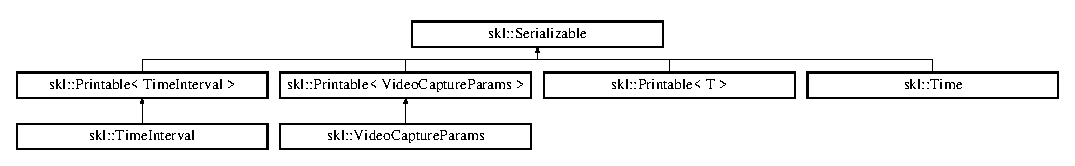
\includegraphics[height=1.787234cm]{classskl_1_1_serializable}
\end{center}
\end{figure}
\subsection*{Public Member Functions}
\begin{DoxyCompactItemize}
\item 
\hypertarget{classskl_1_1_serializable_a94b5cf22d52d2bb6a0fb58e417fa504e}{}\label{classskl_1_1_serializable_a94b5cf22d52d2bb6a0fb58e417fa504e} 
\hyperlink{classskl_1_1_serializable_a94b5cf22d52d2bb6a0fb58e417fa504e}{Serializable} ()
\begin{DoxyCompactList}\small\item\em デフォルトコンストラクタ \end{DoxyCompactList}\item 
\hypertarget{classskl_1_1_serializable_afe0b4a8ee83b34ae2e2b9cd126c662a4}{}\label{classskl_1_1_serializable_afe0b4a8ee83b34ae2e2b9cd126c662a4} 
virtual \hyperlink{classskl_1_1_serializable_afe0b4a8ee83b34ae2e2b9cd126c662a4}{$\sim$\+Serializable} ()
\begin{DoxyCompactList}\small\item\em デストラクタ \end{DoxyCompactList}\item 
\hypertarget{classskl_1_1_serializable_abcf129d50dc5b2f51300645a07ea3a38}{}\label{classskl_1_1_serializable_abcf129d50dc5b2f51300645a07ea3a38} 
virtual std\+::string \hyperlink{classskl_1_1_serializable_abcf129d50dc5b2f51300645a07ea3a38}{get\+Class\+Name} () const
\begin{DoxyCompactList}\small\item\em 関数名を返す \end{DoxyCompactList}\item 
virtual long \hyperlink{classskl_1_1_serializable_a4bd0c82fdb8a663215b54671df1222f2}{serialize} (char $\ast$$\ast$\hyperlink{classskl_1_1_serializable_a1d203d9f0049ce37183a0dcefbc6399a}{buf})
\begin{DoxyCompactList}\small\item\em \hyperlink{classskl_1_1_serializable_a489e26e25bacf78d0dae50f0286c62b5}{\+\_\+buf\+\_\+size()}の返り値を元にbufのメモリ管理をしてから\+\_\+serializeを呼び出す \end{DoxyCompactList}\item 
virtual void \hyperlink{classskl_1_1_serializable_a09f2101bdae407e65e83a286f76cd65f}{deserialize} (const char $\ast$\hyperlink{classskl_1_1_serializable_a1d203d9f0049ce37183a0dcefbc6399a}{buf}, long \hyperlink{classskl_1_1_serializable_a087eb19fada917a42b8411bfecbac0f1}{buf\+\_\+size}=0)
\begin{DoxyCompactList}\small\item\em \hyperlink{classskl_1_1_serializable_a489e26e25bacf78d0dae50f0286c62b5}{\+\_\+buf\+\_\+size()}の返り値を元にbufのメモリ管理をしてから\+\_\+serializeを呼び出す \end{DoxyCompactList}\item 
\hypertarget{classskl_1_1_serializable_aa2710ac29cb9cd325bc8624c5cfc8f7d}{}\label{classskl_1_1_serializable_aa2710ac29cb9cd325bc8624c5cfc8f7d} 
long \hyperlink{classskl_1_1_serializable_aa2710ac29cb9cd325bc8624c5cfc8f7d}{serialized\+Data\+Length} () const
\begin{DoxyCompactList}\small\item\em 直列化された場合のデータのサイズを返す \end{DoxyCompactList}\end{DoxyCompactItemize}
\subsection*{Protected Member Functions}
\begin{DoxyCompactItemize}
\item 
\hypertarget{classskl_1_1_serializable_af62d2ecb4f263cbd1099c6d32e9a0558}{}\label{classskl_1_1_serializable_af62d2ecb4f263cbd1099c6d32e9a0558} 
\hyperlink{classskl_1_1_serializable_af62d2ecb4f263cbd1099c6d32e9a0558}{Serializable} (const \hyperlink{classskl_1_1_serializable}{Serializable} \&other)
\begin{DoxyCompactList}\small\item\em コピーコンストラクタ \end{DoxyCompactList}\item 
\hypertarget{classskl_1_1_serializable_a489e26e25bacf78d0dae50f0286c62b5}{}\label{classskl_1_1_serializable_a489e26e25bacf78d0dae50f0286c62b5} 
virtual long \hyperlink{classskl_1_1_serializable_a489e26e25bacf78d0dae50f0286c62b5}{\+\_\+buf\+\_\+size} () const =0
\begin{DoxyCompactList}\small\item\em \+\_\+serializeで生成される予定のbufの長さを返す \end{DoxyCompactList}\item 
\hypertarget{classskl_1_1_serializable_a1ebe63f20226d3e63fb13e25720b5339}{}\label{classskl_1_1_serializable_a1ebe63f20226d3e63fb13e25720b5339} 
virtual void \hyperlink{classskl_1_1_serializable_a1ebe63f20226d3e63fb13e25720b5339}{\+\_\+serialize} ()=0
\begin{DoxyCompactList}\small\item\em クラスの中身を直列化してメンバ変数のbufに格納する \end{DoxyCompactList}\item 
\hypertarget{classskl_1_1_serializable_a63a6d619bb4d2fd9f5bf423a544e514c}{}\label{classskl_1_1_serializable_a63a6d619bb4d2fd9f5bf423a544e514c} 
virtual void \hyperlink{classskl_1_1_serializable_a63a6d619bb4d2fd9f5bf423a544e514c}{\+\_\+deserialize} (const char $\ast$\hyperlink{classskl_1_1_serializable_a1d203d9f0049ce37183a0dcefbc6399a}{buf}, long \hyperlink{classskl_1_1_serializable_a087eb19fada917a42b8411bfecbac0f1}{buf\+\_\+size})=0
\begin{DoxyCompactList}\small\item\em 直列化されたクラスの中身を読み込む \end{DoxyCompactList}\end{DoxyCompactItemize}
\subsection*{Protected Attributes}
\begin{DoxyCompactItemize}
\item 
\hypertarget{classskl_1_1_serializable_a087eb19fada917a42b8411bfecbac0f1}{}\label{classskl_1_1_serializable_a087eb19fada917a42b8411bfecbac0f1} 
long \hyperlink{classskl_1_1_serializable_a087eb19fada917a42b8411bfecbac0f1}{buf\+\_\+size}
\begin{DoxyCompactList}\small\item\em 直前に呼ばれたserializeで生成されたbufの長さ \end{DoxyCompactList}\item 
\hypertarget{classskl_1_1_serializable_a1d203d9f0049ce37183a0dcefbc6399a}{}\label{classskl_1_1_serializable_a1d203d9f0049ce37183a0dcefbc6399a} 
char $\ast$ \hyperlink{classskl_1_1_serializable_a1d203d9f0049ce37183a0dcefbc6399a}{buf}
\begin{DoxyCompactList}\small\item\em 直前に呼ばれたserializeで生成されたbufの中身 \end{DoxyCompactList}\end{DoxyCompactItemize}


\subsection{Detailed Description}
Black\+Boardを介してデータをやりとりするクラスのインターフェイス 

\subsection{Member Function Documentation}
\hypertarget{classskl_1_1_serializable_a09f2101bdae407e65e83a286f76cd65f}{}\label{classskl_1_1_serializable_a09f2101bdae407e65e83a286f76cd65f} 
\index{skl\+::\+Serializable@{skl\+::\+Serializable}!deserialize@{deserialize}}
\index{deserialize@{deserialize}!skl\+::\+Serializable@{skl\+::\+Serializable}}
\subsubsection{\texorpdfstring{deserialize()}{deserialize()}}
{\footnotesize\ttfamily void skl\+::\+Serializable\+::deserialize (\begin{DoxyParamCaption}\item[{const char $\ast$}]{buf,  }\item[{long}]{buf\+\_\+size = {\ttfamily 0} }\end{DoxyParamCaption})\hspace{0.3cm}{\ttfamily [virtual]}}



\hyperlink{classskl_1_1_serializable_a489e26e25bacf78d0dae50f0286c62b5}{\+\_\+buf\+\_\+size()}の返り値を元にbufのメモリ管理をしてから\+\_\+serializeを呼び出す 


\begin{DoxyParams}{Parameters}
{\em buf} & blackboardに投げるバッファ \\
\hline
\end{DoxyParams}
\begin{DoxyReturn}{Returns}
バッファのバイト長(sizeof(char)x\+NのN) 
\end{DoxyReturn}
\hypertarget{classskl_1_1_serializable_a4bd0c82fdb8a663215b54671df1222f2}{}\label{classskl_1_1_serializable_a4bd0c82fdb8a663215b54671df1222f2} 
\index{skl\+::\+Serializable@{skl\+::\+Serializable}!serialize@{serialize}}
\index{serialize@{serialize}!skl\+::\+Serializable@{skl\+::\+Serializable}}
\subsubsection{\texorpdfstring{serialize()}{serialize()}}
{\footnotesize\ttfamily long skl\+::\+Serializable\+::serialize (\begin{DoxyParamCaption}\item[{char $\ast$$\ast$}]{buf }\end{DoxyParamCaption})\hspace{0.3cm}{\ttfamily [virtual]}}



\hyperlink{classskl_1_1_serializable_a489e26e25bacf78d0dae50f0286c62b5}{\+\_\+buf\+\_\+size()}の返り値を元にbufのメモリ管理をしてから\+\_\+serializeを呼び出す 


\begin{DoxyParams}{Parameters}
{\em buf} & blackboardに投げるバッファ \\
\hline
\end{DoxyParams}
\begin{DoxyReturn}{Returns}
バッファのバイト長(sizeof(char)x\+NのN) 
\end{DoxyReturn}


The documentation for this class was generated from the following files\+:\begin{DoxyCompactItemize}
\item 
Core/include/\hyperlink{_serializable_8h}{Serializable.\+h}\item 
Core/src/\hyperlink{_serializable_8cpp}{Serializable.\+cpp}\end{DoxyCompactItemize}

\hypertarget{classskl_1_1_short_memory_moments}{}\section{skl\+:\+:Short\+Memory\+Moments$<$ Sample, N $>$ Class Template Reference}
\label{classskl_1_1_short_memory_moments}\index{skl\+::\+Short\+Memory\+Moments$<$ Sample, N $>$@{skl\+::\+Short\+Memory\+Moments$<$ Sample, N $>$}}


一定区間の長さのn次モーメントを計算・保存するクラス  




{\ttfamily \#include $<$Short\+Memory\+Moments.\+hpp$>$}

\subsection*{Public Member Functions}
\begin{DoxyCompactItemize}
\item 
\hypertarget{classskl_1_1_short_memory_moments_ae6ca957d4f287d189762b13cb723c24c}{}\label{classskl_1_1_short_memory_moments_ae6ca957d4f287d189762b13cb723c24c} 
{\bfseries Short\+Memory\+Moments} (size\+\_\+t memory\+\_\+length=U\+I\+N\+T\+\_\+\+M\+AX)
\item 
\hypertarget{classskl_1_1_short_memory_moments_a0310614e8dc620abf8c8f878d193a6f8}{}\label{classskl_1_1_short_memory_moments_a0310614e8dc620abf8c8f878d193a6f8} 
void {\bfseries clear} ()
\item 
\hypertarget{classskl_1_1_short_memory_moments_aa5a5cb03966c5b538e9ccabdac781b13}{}\label{classskl_1_1_short_memory_moments_aa5a5cb03966c5b538e9ccabdac781b13} 
\hyperlink{classskl_1_1_short_memory_moments}{Short\+Memory\+Moments}$<$ Sample, N $>$ \& {\bfseries operator=} (const \hyperlink{classskl_1_1_short_memory_moments}{Short\+Memory\+Moments}$<$ Sample, N $>$ \&other)
\item 
\hypertarget{classskl_1_1_short_memory_moments_a9dcd1b0da5df9ecb5a3f3ebc65c9c621}{}\label{classskl_1_1_short_memory_moments_a9dcd1b0da5df9ecb5a3f3ebc65c9c621} 
void {\bfseries operator()} (const Sample \&sample)
\item 
\hypertarget{classskl_1_1_short_memory_moments_ab9b55dadd93668a196175116ed1080b4}{}\label{classskl_1_1_short_memory_moments_ab9b55dadd93668a196175116ed1080b4} 
{\footnotesize template$<$typename Iter $>$ }\\void {\bfseries operator()} (Iter begin, Iter end)
\item 
\hypertarget{classskl_1_1_short_memory_moments_aec6d2eac7efa71ccf67f170e33da5830}{}\label{classskl_1_1_short_memory_moments_aec6d2eac7efa71ccf67f170e33da5830} 
void {\bfseries push} (const Sample \&sample)
\item 
\hypertarget{classskl_1_1_short_memory_moments_ade602d5aa181bf3d5d200cf4a63bc386}{}\label{classskl_1_1_short_memory_moments_ade602d5aa181bf3d5d200cf4a63bc386} 
Sample {\bfseries operator\mbox{[}$\,$\mbox{]}} (size\+\_\+t i) const
\item 
\hypertarget{classskl_1_1_short_memory_moments_a39099e1827b907bd909e8fe1f5b2c60a}{}\label{classskl_1_1_short_memory_moments_a39099e1827b907bd909e8fe1f5b2c60a} 
Sample {\bfseries sum} () const
\item 
\hypertarget{classskl_1_1_short_memory_moments_a5d0707bc160c2651e1dbabe2b7175477}{}\label{classskl_1_1_short_memory_moments_a5d0707bc160c2651e1dbabe2b7175477} 
Sample {\bfseries mean} () const
\item 
\hypertarget{classskl_1_1_short_memory_moments_a6e5c15f9794e48975eb3e73789413a14}{}\label{classskl_1_1_short_memory_moments_a6e5c15f9794e48975eb3e73789413a14} 
Sample {\bfseries variance} () const
\item 
\hypertarget{classskl_1_1_short_memory_moments_aab5a76ac31752abf4bc0b2f98518bed0}{}\label{classskl_1_1_short_memory_moments_aab5a76ac31752abf4bc0b2f98518bed0} 
Sample {\bfseries stddev} () const
\item 
\hypertarget{classskl_1_1_short_memory_moments_a4002576cceb297b0a99754ce5154fc92}{}\label{classskl_1_1_short_memory_moments_a4002576cceb297b0a99754ce5154fc92} 
size\+\_\+t {\bfseries size} () const
\item 
\hypertarget{classskl_1_1_short_memory_moments_a30182a68815880321af4ab3001711f62}{}\label{classskl_1_1_short_memory_moments_a30182a68815880321af4ab3001711f62} 
void {\bfseries memory\+\_\+length} (size\+\_\+t \+\_\+\+\_\+memory\+\_\+length)
\item 
\hypertarget{classskl_1_1_short_memory_moments_a524b3def4dc523479423fd574d8c7c69}{}\label{classskl_1_1_short_memory_moments_a524b3def4dc523479423fd574d8c7c69} 
size\+\_\+t {\bfseries memory\+\_\+length} () const
\item 
\hypertarget{classskl_1_1_short_memory_moments_a68ce6b75f502bbe9cfa2cc61a3c2f533}{}\label{classskl_1_1_short_memory_moments_a68ce6b75f502bbe9cfa2cc61a3c2f533} 
const std\+::list$<$ Sample $>$ \& {\bfseries short\+\_\+memory} () const
\item 
\hypertarget{classskl_1_1_short_memory_moments_accb65fb4409f56d1a2d8849038ba700c}{}\label{classskl_1_1_short_memory_moments_accb65fb4409f56d1a2d8849038ba700c} 
std\+::list$<$ Sample $>$ \& {\bfseries short\+\_\+memory} ()
\end{DoxyCompactItemize}
\subsection*{Protected Member Functions}
\begin{DoxyCompactItemize}
\item 
\hypertarget{classskl_1_1_short_memory_moments_a7ecfa55b2e215c8920c4ac3b5771ac6d}{}\label{classskl_1_1_short_memory_moments_a7ecfa55b2e215c8920c4ac3b5771ac6d} 
void {\bfseries pop} ()
\end{DoxyCompactItemize}
\subsection*{Protected Attributes}
\begin{DoxyCompactItemize}
\item 
\hypertarget{classskl_1_1_short_memory_moments_a665bdcc39d02f026a3d4004e9125320b}{}\label{classskl_1_1_short_memory_moments_a665bdcc39d02f026a3d4004e9125320b} 
std\+::list$<$ Sample $>$ {\bfseries \+\_\+short\+\_\+memory}
\item 
\hypertarget{classskl_1_1_short_memory_moments_a3f30e699be2e68358aaad18a2cb02b10}{}\label{classskl_1_1_short_memory_moments_a3f30e699be2e68358aaad18a2cb02b10} 
std\+::vector$<$ Sample $>$ {\bfseries \+\_\+moments}
\item 
\hypertarget{classskl_1_1_short_memory_moments_a86cf2e73d37620bf7dce0a26c8212324}{}\label{classskl_1_1_short_memory_moments_a86cf2e73d37620bf7dce0a26c8212324} 
size\+\_\+t {\bfseries \+\_\+memory\+\_\+length}
\end{DoxyCompactItemize}


\subsection{Detailed Description}
\subsubsection*{template$<$typename Sample = double, unsigned int N = 2$>$\newline
class skl\+::\+Short\+Memory\+Moments$<$ Sample, N $>$}

一定区間の長さのn次モーメントを計算・保存するクラス 

The documentation for this class was generated from the following file\+:\begin{DoxyCompactItemize}
\item 
Core/include/Short\+Memory\+Moments.\+hpp\end{DoxyCompactItemize}

\hypertarget{classskl_1_1_particle_filter_1_1_state}{}\section{skl\+:\+:Particle\+Filter$<$ Observation, Likelihood\+Calc\+Functor $>$\+:\+:State Class Reference}
\label{classskl_1_1_particle_filter_1_1_state}\index{skl\+::\+Particle\+Filter$<$ Observation, Likelihood\+Calc\+Functor $>$\+::\+State@{skl\+::\+Particle\+Filter$<$ Observation, Likelihood\+Calc\+Functor $>$\+::\+State}}
\subsection*{Public Member Functions}
\begin{DoxyCompactItemize}
\item 
\hypertarget{classskl_1_1_particle_filter_1_1_state_a6ff704b75497738e21cfc10aa367a11b}{}\label{classskl_1_1_particle_filter_1_1_state_a6ff704b75497738e21cfc10aa367a11b} 
{\bfseries State} (size\+\_\+t dim)
\item 
\hypertarget{classskl_1_1_particle_filter_1_1_state_ac6edc939c6cf03c0d3ec9b058e92e151}{}\label{classskl_1_1_particle_filter_1_1_state_ac6edc939c6cf03c0d3ec9b058e92e151} 
{\bfseries State} (size\+\_\+t dim, float $\ast$data)
\item 
\hypertarget{classskl_1_1_particle_filter_1_1_state_a7c1cc84a4a62cd5196374628e1d38cc1}{}\label{classskl_1_1_particle_filter_1_1_state_a7c1cc84a4a62cd5196374628e1d38cc1} 
{\bfseries State} (const \hyperlink{classskl_1_1_particle_filter_1_1_state}{State} \&other)
\item 
\hypertarget{classskl_1_1_particle_filter_1_1_state_a104052be4ddae96d6bf5d3800cc85120}{}\label{classskl_1_1_particle_filter_1_1_state_a104052be4ddae96d6bf5d3800cc85120} 
\hyperlink{classskl_1_1_particle_filter_1_1_state}{State} {\bfseries clone} () const
\item 
\hypertarget{classskl_1_1_particle_filter_1_1_state_a90c79606220afc69f15c2d4db6567e2b}{}\label{classskl_1_1_particle_filter_1_1_state_a90c79606220afc69f15c2d4db6567e2b} 
size\+\_\+t {\bfseries dim} () const
\end{DoxyCompactItemize}
\subsection*{Public Attributes}
\begin{DoxyCompactItemize}
\item 
\hypertarget{classskl_1_1_particle_filter_1_1_state_aaee6a1cb6e79d44ce7afc6506adfd393}{}\label{classskl_1_1_particle_filter_1_1_state_aaee6a1cb6e79d44ce7afc6506adfd393} 
cv\+::\+Ptr$<$ float $>$ {\bfseries data}
\end{DoxyCompactItemize}
\subsection*{Protected Attributes}
\begin{DoxyCompactItemize}
\item 
\hypertarget{classskl_1_1_particle_filter_1_1_state_acd1a54086df7417b368c74c6709b169a}{}\label{classskl_1_1_particle_filter_1_1_state_acd1a54086df7417b368c74c6709b169a} 
size\+\_\+t {\bfseries \+\_\+dim}
\end{DoxyCompactItemize}


The documentation for this class was generated from the following file\+:\begin{DoxyCompactItemize}
\item 
Open\+C\+V/include/Particle\+Filter.\+hpp\end{DoxyCompactItemize}

\hypertarget{classskl_1_1_static_region_detector}{}\section{skl\+:\+:Static\+Region\+Detector Class Reference}
\label{classskl_1_1_static_region_detector}\index{skl\+::\+Static\+Region\+Detector@{skl\+::\+Static\+Region\+Detector}}
Inheritance diagram for skl\+:\+:Static\+Region\+Detector\+:\begin{figure}[H]
\begin{center}
\leavevmode
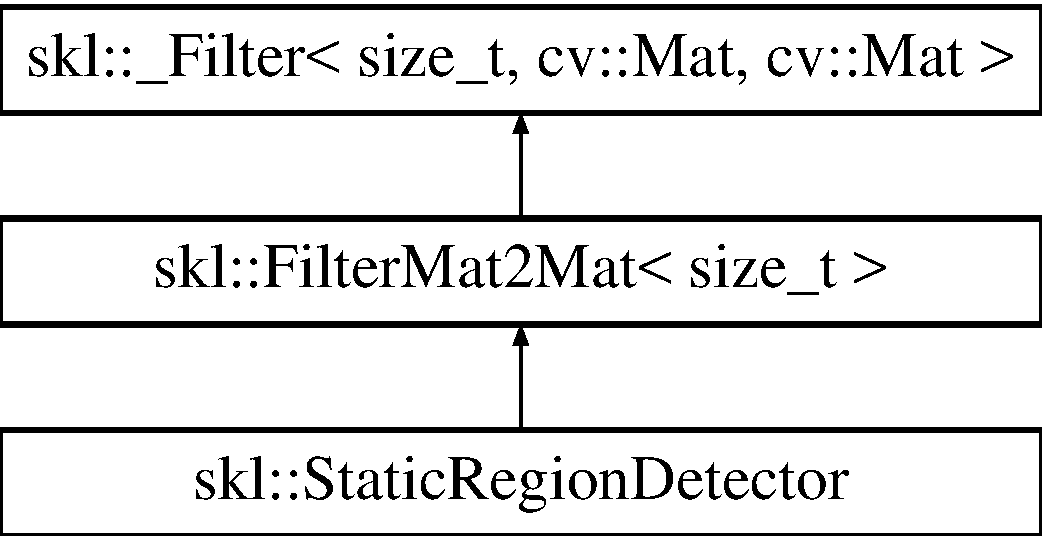
\includegraphics[height=3.000000cm]{classskl_1_1_static_region_detector}
\end{center}
\end{figure}
\subsection*{Public Member Functions}
\begin{DoxyCompactItemize}
\item 
\hypertarget{classskl_1_1_static_region_detector_af9aad28d28e257629fcf3fcb5493f233}{}\label{classskl_1_1_static_region_detector_af9aad28d28e257629fcf3fcb5493f233} 
{\bfseries Static\+Region\+Detector} (double thresh=0.\+95, size\+\_\+t life\+\_\+time=1)
\item 
\hypertarget{classskl_1_1_static_region_detector_aa1da9a506f8ba01ca425c2ffe2a86e1f}{}\label{classskl_1_1_static_region_detector_aa1da9a506f8ba01ca425c2ffe2a86e1f} 
void {\bfseries set\+Param} (double thresh, size\+\_\+t life\+\_\+time=1)
\item 
\hypertarget{classskl_1_1_static_region_detector_aadb27183ceabe4245bc8d66cbde3bd09}{}\label{classskl_1_1_static_region_detector_aadb27183ceabe4245bc8d66cbde3bd09} 
size\+\_\+t {\bfseries compute} (const cv\+::\+Mat \&region\+\_\+labels, const cv\+::\+Mat \&mask, cv\+::\+Mat \&object\+\_\+labels)
\item 
\hypertarget{classskl_1_1_static_region_detector_ae7fb3fd041ae662d003a5e51e333743c}{}\label{classskl_1_1_static_region_detector_ae7fb3fd041ae662d003a5e51e333743c} 
void {\bfseries clear} ()
\end{DoxyCompactItemize}
\subsection*{Protected Member Functions}
\begin{DoxyCompactItemize}
\item 
\hypertarget{classskl_1_1_static_region_detector_aa3cff990aee433457901e8a75a575511}{}\label{classskl_1_1_static_region_detector_aa3cff990aee433457901e8a75a575511} 
std\+::vector$<$ bool $>$ {\bfseries update\+\_\+object\+\_\+life\+\_\+map} (const std\+::vector$<$ size\+\_\+t $>$ \&current\+\_\+object\+\_\+areas, const std\+::vector$<$ size\+\_\+t $>$ \&prev\+\_\+object\+\_\+areas, std\+::vector$<$ std\+::vector$<$ size\+\_\+t $>$ $>$ \&cross\+\_\+area\+\_\+mat)
\item 
\hypertarget{classskl_1_1_static_region_detector_ac3bb59ccc2fd2924e9629aa0ad7f81e4}{}\label{classskl_1_1_static_region_detector_ac3bb59ccc2fd2924e9629aa0ad7f81e4} 
double {\bfseries calc\+Score} (double area1, double area2, double cross\+\_\+area) const
\end{DoxyCompactItemize}
\subsection*{Protected Attributes}
\begin{DoxyCompactItemize}
\item 
\hypertarget{classskl_1_1_static_region_detector_a25e5612d213f6bb3c88619c18dd4c34f}{}\label{classskl_1_1_static_region_detector_a25e5612d213f6bb3c88619c18dd4c34f} 
double {\bfseries thresh}
\item 
\hypertarget{classskl_1_1_static_region_detector_a7834bd2105ac6283f300fcba18654bee}{}\label{classskl_1_1_static_region_detector_a7834bd2105ac6283f300fcba18654bee} 
int {\bfseries life\+\_\+time}
\item 
\hypertarget{classskl_1_1_static_region_detector_aa098c876dadb30192223065f08aa190a}{}\label{classskl_1_1_static_region_detector_aa098c876dadb30192223065f08aa190a} 
cv\+::\+Mat {\bfseries prev\+\_\+labels}
\item 
\hypertarget{classskl_1_1_static_region_detector_aad91aa7788b52402a7f0bdb0bf7fcb9f}{}\label{classskl_1_1_static_region_detector_aad91aa7788b52402a7f0bdb0bf7fcb9f} 
std\+::vector$<$ size\+\_\+t $>$ {\bfseries prev\+\_\+object\+\_\+areas}
\item 
\hypertarget{classskl_1_1_static_region_detector_a23d3aa54be57f5f856aa28c0a6799f6a}{}\label{classskl_1_1_static_region_detector_a23d3aa54be57f5f856aa28c0a6799f6a} 
std\+::map$<$ size\+\_\+t, size\+\_\+t $>$ {\bfseries object\+\_\+life\+\_\+map}
\end{DoxyCompactItemize}


The documentation for this class was generated from the following files\+:\begin{DoxyCompactItemize}
\item 
Open\+C\+V/include/Static\+Region\+Detector.\+h\item 
Open\+C\+V/src/Static\+Region\+Detector.\+cpp\end{DoxyCompactItemize}

\hypertarget{classskl_1_1_stop_watch}{}\section{skl\+:\+:Stop\+Watch Class Reference}
\label{classskl_1_1_stop_watch}\index{skl\+::\+Stop\+Watch@{skl\+::\+Stop\+Watch}}


実行時間を計測するクラス(D\+E\+B\+UG or S\+T\+O\+P\+\_\+\+W\+A\+T\+C\+Hが定義されている時のみ動作)  




{\ttfamily \#include $<$Stop\+Watch.\+h$>$}

\subsection*{Public Member Functions}
\begin{DoxyCompactItemize}
\item 
\hypertarget{classskl_1_1_stop_watch_ad715945060eeb23baa3c036ad19b1edb}{}\label{classskl_1_1_stop_watch_ad715945060eeb23baa3c036ad19b1edb} 
\hyperlink{classskl_1_1_stop_watch_ad715945060eeb23baa3c036ad19b1edb}{Stop\+Watch} ()
\begin{DoxyCompactList}\small\item\em デフォルトコンストラクタ \end{DoxyCompactList}\item 
\hypertarget{classskl_1_1_stop_watch_a223ec0da71dd0bc4f2b14d1af44bf20a}{}\label{classskl_1_1_stop_watch_a223ec0da71dd0bc4f2b14d1af44bf20a} 
virtual \hyperlink{classskl_1_1_stop_watch_a223ec0da71dd0bc4f2b14d1af44bf20a}{$\sim$\+Stop\+Watch} ()
\begin{DoxyCompactList}\small\item\em デストラクタ \end{DoxyCompactList}\item 
\hypertarget{classskl_1_1_stop_watch_a09a3c8f9ab03d7b28e4f8b90a833974e}{}\label{classskl_1_1_stop_watch_a09a3c8f9ab03d7b28e4f8b90a833974e} 
void \hyperlink{classskl_1_1_stop_watch_a09a3c8f9ab03d7b28e4f8b90a833974e}{start} ()
\begin{DoxyCompactList}\small\item\em start measure \end{DoxyCompactList}\item 
\hypertarget{classskl_1_1_stop_watch_a9f944c617ed495f2d77e3edee204e29b}{}\label{classskl_1_1_stop_watch_a9f944c617ed495f2d77e3edee204e29b} 
\hyperlink{classskl_1_1_time_interval}{Time\+Interval} \hyperlink{classskl_1_1_stop_watch_a9f944c617ed495f2d77e3edee204e29b}{stop} ()
\begin{DoxyCompactList}\small\item\em stop measure \end{DoxyCompactList}\item 
\hypertarget{classskl_1_1_stop_watch_a1c0dcc57c615559f24bc9f8759271a9d}{}\label{classskl_1_1_stop_watch_a1c0dcc57c615559f24bc9f8759271a9d} 
void {\bfseries reset} ()
\item 
\hypertarget{classskl_1_1_stop_watch_aef15961ff53acf72b87811599fac1e20}{}\label{classskl_1_1_stop_watch_aef15961ff53acf72b87811599fac1e20} 
const std\+::vector$<$ \hyperlink{classskl_1_1_time_interval}{Time\+Interval} $>$ \& {\bfseries lap\+\_\+time} () const
\item 
\hypertarget{classskl_1_1_stop_watch_a534efc1c95686b88f97f3712b6441f9c}{}\label{classskl_1_1_stop_watch_a534efc1c95686b88f97f3712b6441f9c} 
\hyperlink{classskl_1_1_time_interval}{Time\+Interval} {\bfseries lap\+\_\+time} (size\+\_\+t i) const
\item 
\hypertarget{classskl_1_1_stop_watch_a88365867fd14c9da7ae53201370a9b02}{}\label{classskl_1_1_stop_watch_a88365867fd14c9da7ae53201370a9b02} 
\hyperlink{classskl_1_1_time_interval}{Time\+Interval} {\bfseries lap} ()
\item 
\hypertarget{classskl_1_1_stop_watch_aafb3337fe4778a94ee4a669338b8cd72}{}\label{classskl_1_1_stop_watch_aafb3337fe4778a94ee4a669338b8cd72} 
\hyperlink{classskl_1_1_time_interval}{Time\+Interval} {\bfseries elapsed\+Time} () const
\item 
\hypertarget{classskl_1_1_stop_watch_ab2a25335e19110c6deb98ea12af02f1a}{}\label{classskl_1_1_stop_watch_ab2a25335e19110c6deb98ea12af02f1a} 
size\+\_\+t {\bfseries record\+\_\+num} () const
\item 
\hypertarget{classskl_1_1_stop_watch_aea3486e95f37ed932be6d2ced2d116d2}{}\label{classskl_1_1_stop_watch_aea3486e95f37ed932be6d2ced2d116d2} 
void {\bfseries clear} ()
\end{DoxyCompactItemize}
\subsection*{Protected Attributes}
\begin{DoxyCompactItemize}
\item 
\hypertarget{classskl_1_1_stop_watch_a73c3969e2539b2a7321fd52bb8f62143}{}\label{classskl_1_1_stop_watch_a73c3969e2539b2a7321fd52bb8f62143} 
\hyperlink{classskl_1_1_time}{Time} {\bfseries base\+\_\+time}
\item 
\hypertarget{classskl_1_1_stop_watch_a888a4bdf053fac5ea7d2dd0b1c076920}{}\label{classskl_1_1_stop_watch_a888a4bdf053fac5ea7d2dd0b1c076920} 
std\+::vector$<$ \hyperlink{classskl_1_1_time_interval}{Time\+Interval} $>$ {\bfseries lap\+\_\+times}
\end{DoxyCompactItemize}


\subsection{Detailed Description}
実行時間を計測するクラス(D\+E\+B\+UG or S\+T\+O\+P\+\_\+\+W\+A\+T\+C\+Hが定義されている時のみ動作) 

The documentation for this class was generated from the following files\+:\begin{DoxyCompactItemize}
\item 
Core/include/\hyperlink{_stop_watch_8h}{Stop\+Watch.\+h}\item 
Core/src/\hyperlink{_stop_watch_8cpp}{Stop\+Watch.\+cpp}\end{DoxyCompactItemize}

\hypertarget{classskl_1_1gpu_1_1_table_object_manager}{}\section{skl\+:\+:gpu\+:\+:Table\+Object\+Manager Class Reference}
\label{classskl_1_1gpu_1_1_table_object_manager}\index{skl\+::gpu\+::\+Table\+Object\+Manager@{skl\+::gpu\+::\+Table\+Object\+Manager}}
Inheritance diagram for skl\+:\+:gpu\+:\+:Table\+Object\+Manager\+:\begin{figure}[H]
\begin{center}
\leavevmode
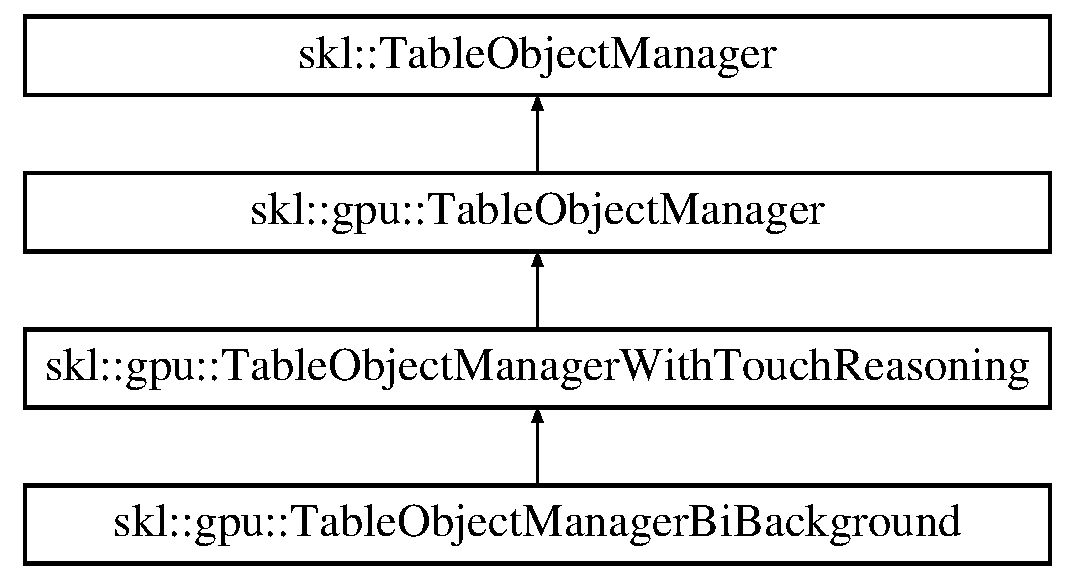
\includegraphics[height=4.000000cm]{classskl_1_1gpu_1_1_table_object_manager}
\end{center}
\end{figure}
\subsection*{Public Types}
\begin{DoxyCompactItemize}
\item 
\hypertarget{classskl_1_1gpu_1_1_table_object_manager_a75b519bccc987044293a735eef7f28af}{}\label{classskl_1_1gpu_1_1_table_object_manager_a75b519bccc987044293a735eef7f28af} 
typedef \hyperlink{classskl_1_1_filter_mat2_mat}{Filter\+Mat2\+Mat}$<$ size\+\_\+t $>$ {\bfseries Region\+Labeling\+Algorithm}
\item 
\hypertarget{classskl_1_1gpu_1_1_table_object_manager_a2baac34bf45c2953749a6c4bc283365a}{}\label{classskl_1_1gpu_1_1_table_object_manager_a2baac34bf45c2953749a6c4bc283365a} 
typedef \hyperlink{classskl_1_1_filter_mat2_mat}{Filter\+Mat2\+Mat}$<$ std\+::list$<$ size\+\_\+t $>$ $>$ {\bfseries Human\+Detector}
\end{DoxyCompactItemize}
\subsection*{Public Member Functions}
\begin{DoxyCompactItemize}
\item 
\hypertarget{classskl_1_1gpu_1_1_table_object_manager_a0ff30de4687ffad72163fc748fc551e5}{}\label{classskl_1_1gpu_1_1_table_object_manager_a0ff30de4687ffad72163fc748fc551e5} 
{\bfseries Table\+Object\+Manager} (float \+\_\+\+\_\+learning\+\_\+rate=0.\+05, cv\+::\+Ptr$<$ \hyperlink{classskl_1_1gpu_1_1_tex_cut}{skl\+::gpu\+::\+Tex\+Cut} $>$ bgs\+\_\+algo=new \hyperlink{classskl_1_1gpu_1_1_tex_cut}{skl\+::gpu\+::\+Tex\+Cut}(), cv\+::\+Ptr$<$ \hyperlink{classskl_1_1_filter_mat2_mat}{Region\+Labeling\+Algorithm} $>$ region\+\_\+labeling\+\_\+algo=new \hyperlink{classskl_1_1_region_labeling_simple}{Region\+Labeling\+Simple}(), cv\+::\+Ptr$<$ \hyperlink{classskl_1_1_filter_mat2_mat}{Human\+Detector} $>$ human\+\_\+detect\+\_\+algo=new \hyperlink{classskl_1_1_human_detector_workspace_end}{Human\+Detector\+Workspace\+End}(), cv\+::\+Ptr$<$ \hyperlink{classskl_1_1_filter_mat2_mat}{Region\+Labeling\+Algorithm} $>$ static\+\_\+region\+\_\+detect\+\_\+algo=new \hyperlink{classskl_1_1_static_region_detector}{Static\+Region\+Detector}(), cv\+::\+Ptr$<$ \hyperlink{classskl_1_1_patch_model}{Patch\+Model} $>$ patch\+\_\+model=new \hyperlink{classskl_1_1_patch_model}{Patch\+Model}())
\item 
\hypertarget{classskl_1_1gpu_1_1_table_object_manager_a6c57e723de495cf9be622b249a612958}{}\label{classskl_1_1gpu_1_1_table_object_manager_a6c57e723de495cf9be622b249a612958} 
virtual void {\bfseries compute} (const cv\+::\+Mat \&src, const cv\+::gpu\+::\+Gpu\+Mat \&src\+\_\+gpu, cv\+::\+Mat \&human, std\+::vector$<$ size\+\_\+t $>$ \&put\+\_\+objects, std\+::vector$<$ size\+\_\+t $>$ \&taken\+\_\+objects)
\item 
\hypertarget{classskl_1_1gpu_1_1_table_object_manager_a7b7dcddbfa9228f34ca7ebd57626bf8d}{}\label{classskl_1_1gpu_1_1_table_object_manager_a7b7dcddbfa9228f34ca7ebd57626bf8d} 
const cv\+::\+Ptr$<$ \hyperlink{classskl_1_1gpu_1_1_tex_cut}{skl\+::gpu\+::\+Tex\+Cut} $>$ \& {\bfseries bgs\+\_\+algo} () const
\item 
\hypertarget{classskl_1_1gpu_1_1_table_object_manager_a7ef64b9fffa6e95946c73431ba6207c4}{}\label{classskl_1_1gpu_1_1_table_object_manager_a7ef64b9fffa6e95946c73431ba6207c4} 
void {\bfseries bgs\+\_\+algo} (const cv\+::\+Ptr$<$ \hyperlink{classskl_1_1gpu_1_1_tex_cut}{skl\+::gpu\+::\+Tex\+Cut} $>$ \&\+\_\+\+\_\+bgs\+\_\+algo)
\end{DoxyCompactItemize}
\subsection*{Protected Member Functions}
\begin{DoxyCompactItemize}
\item 
\hypertarget{classskl_1_1gpu_1_1_table_object_manager_a54ae21fe001b5dfe605004be798ddd05}{}\label{classskl_1_1gpu_1_1_table_object_manager_a54ae21fe001b5dfe605004be798ddd05} 
virtual void {\bfseries bg\+\_\+subtract} (const cv\+::gpu\+::\+Gpu\+Mat \&src, cv\+::\+Mat \&dest)
\item 
\hypertarget{classskl_1_1gpu_1_1_table_object_manager_a39dfb2a4da44e15fc82acaf4e9c2ada1}{}\label{classskl_1_1gpu_1_1_table_object_manager_a39dfb2a4da44e15fc82acaf4e9c2ada1} 
virtual void {\bfseries bg\+\_\+update} (const cv\+::\+Mat \&src, const cv\+::\+Mat \&non\+\_\+update\+\_\+mask)
\end{DoxyCompactItemize}
\subsection*{Protected Attributes}
\begin{DoxyCompactItemize}
\item 
\hypertarget{classskl_1_1gpu_1_1_table_object_manager_a799ccd9c25994262f4016c0c74486a1d}{}\label{classskl_1_1gpu_1_1_table_object_manager_a799ccd9c25994262f4016c0c74486a1d} 
cv\+::\+Ptr$<$ \hyperlink{classskl_1_1gpu_1_1_tex_cut}{skl\+::gpu\+::\+Tex\+Cut} $>$ {\bfseries \+\_\+bgs\+\_\+algo}
\item 
\hypertarget{classskl_1_1gpu_1_1_table_object_manager_a70c2b67b0afe1ad3ac4a2d7209e1b142}{}\label{classskl_1_1gpu_1_1_table_object_manager_a70c2b67b0afe1ad3ac4a2d7209e1b142} 
cv\+::gpu\+::\+Gpu\+Mat {\bfseries bg\+\_\+for\+\_\+texcut}
\item 
\hypertarget{classskl_1_1gpu_1_1_table_object_manager_ab48f43306b5113b29550519495d38482}{}\label{classskl_1_1gpu_1_1_table_object_manager_ab48f43306b5113b29550519495d38482} 
bool {\bfseries do\+Set\+Background}
\item 
\hypertarget{classskl_1_1gpu_1_1_table_object_manager_aab6b340446a6a7d590d30d02744d45bf}{}\label{classskl_1_1gpu_1_1_table_object_manager_aab6b340446a6a7d590d30d02744d45bf} 
cv\+::gpu\+::\+Cuda\+Mem {\bfseries \+\_\+page\+\_\+locked\+\_\+bg}
\end{DoxyCompactItemize}
\subsection*{Additional Inherited Members}


The documentation for this class was generated from the following files\+:\begin{DoxyCompactItemize}
\item 
Open\+C\+V\+G\+P\+U/include/Table\+Object\+Manager\+Gpu.\+h\item 
Open\+C\+V\+G\+P\+U/src/Table\+Object\+Manager.\+cpp\end{DoxyCompactItemize}

\hypertarget{classskl_1_1_table_object_manager}{}\section{skl\+:\+:Table\+Object\+Manager Class Reference}
\label{classskl_1_1_table_object_manager}\index{skl\+::\+Table\+Object\+Manager@{skl\+::\+Table\+Object\+Manager}}
Inheritance diagram for skl\+:\+:Table\+Object\+Manager\+:\begin{figure}[H]
\begin{center}
\leavevmode
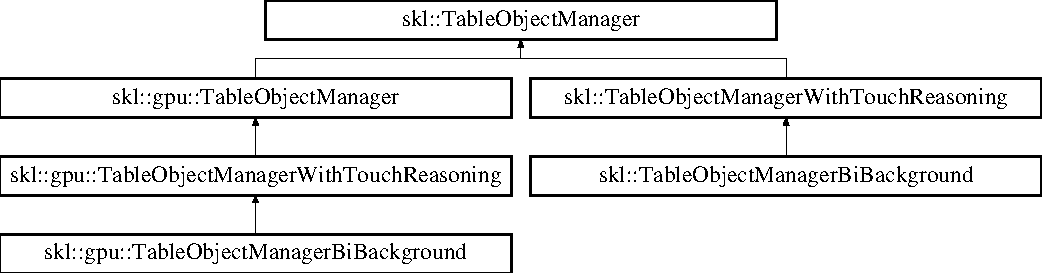
\includegraphics[height=3.672131cm]{classskl_1_1_table_object_manager}
\end{center}
\end{figure}
\subsection*{Public Types}
\begin{DoxyCompactItemize}
\item 
\hypertarget{classskl_1_1_table_object_manager_a422d00c4412bfcaa566575392bf74a34}{}\label{classskl_1_1_table_object_manager_a422d00c4412bfcaa566575392bf74a34} 
typedef \hyperlink{classskl_1_1_filter_mat2_mat}{Filter\+Mat2\+Mat}$<$ size\+\_\+t $>$ {\bfseries Region\+Labeling\+Algorithm}
\item 
\hypertarget{classskl_1_1_table_object_manager_a67feba55350b7494b2fdd7c85542df26}{}\label{classskl_1_1_table_object_manager_a67feba55350b7494b2fdd7c85542df26} 
typedef \hyperlink{classskl_1_1_filter_mat2_mat}{Filter\+Mat2\+Mat}$<$ std\+::list$<$ size\+\_\+t $>$ $>$ {\bfseries Human\+Detector}
\end{DoxyCompactItemize}
\subsection*{Public Member Functions}
\begin{DoxyCompactItemize}
\item 
\hypertarget{classskl_1_1_table_object_manager_a2be8e2e0549d00e2294c7afcaf09925a}{}\label{classskl_1_1_table_object_manager_a2be8e2e0549d00e2294c7afcaf09925a} 
{\bfseries Table\+Object\+Manager} (float \+\_\+\+\_\+learning\+\_\+rate=0.\+05, cv\+::\+Ptr$<$ \hyperlink{classskl_1_1_background_subtract_algorithm}{Background\+Subtract\+Algorithm} $>$ bgs\+\_\+algo=new \hyperlink{classskl_1_1_tex_cut}{Tex\+Cut}(), cv\+::\+Ptr$<$ \hyperlink{classskl_1_1_filter_mat2_mat}{Region\+Labeling\+Algorithm} $>$ region\+\_\+labeling\+\_\+algo=new \hyperlink{classskl_1_1_region_labeling_simple}{Region\+Labeling\+Simple}(), cv\+::\+Ptr$<$ \hyperlink{classskl_1_1_filter_mat2_mat}{Human\+Detector} $>$ human\+\_\+detect\+\_\+algo=new \hyperlink{classskl_1_1_human_detector_workspace_end}{Human\+Detector\+Workspace\+End}(), cv\+::\+Ptr$<$ \hyperlink{classskl_1_1_filter_mat2_mat}{Region\+Labeling\+Algorithm} $>$ static\+\_\+region\+\_\+detect\+\_\+algo=new \hyperlink{classskl_1_1_static_region_detector}{Static\+Region\+Detector}(), cv\+::\+Ptr$<$ \hyperlink{classskl_1_1_patch_model}{Patch\+Model} $>$ patch\+\_\+model=new \hyperlink{classskl_1_1_patch_model}{Patch\+Model}())
\item 
\hypertarget{classskl_1_1_table_object_manager_a523dae27c643a43c2e1cac927d468ded}{}\label{classskl_1_1_table_object_manager_a523dae27c643a43c2e1cac927d468ded} 
void {\bfseries compute} (const cv\+::\+Mat \&src, cv\+::\+Mat \&human, std\+::vector$<$ size\+\_\+t $>$ \&put\+\_\+objects, std\+::vector$<$ size\+\_\+t $>$ \&taken\+\_\+objects)
\item 
\hypertarget{classskl_1_1_table_object_manager_acc23bf35d4261ec51183024ee8369dcb}{}\label{classskl_1_1_table_object_manager_acc23bf35d4261ec51183024ee8369dcb} 
const cv\+::\+Ptr$<$ \hyperlink{classskl_1_1_background_subtract_algorithm}{Background\+Subtract\+Algorithm} $>$ \& {\bfseries bgs\+\_\+algo} () const
\item 
\hypertarget{classskl_1_1_table_object_manager_a3f4b53cccceb62c45e20296b6ef82229}{}\label{classskl_1_1_table_object_manager_a3f4b53cccceb62c45e20296b6ef82229} 
void {\bfseries bgs\+\_\+algo} (const cv\+::\+Ptr$<$ \hyperlink{classskl_1_1_background_subtract_algorithm}{Background\+Subtract\+Algorithm} $>$ \&\+\_\+\+\_\+bgs\+\_\+algo)
\item 
\hypertarget{classskl_1_1_table_object_manager_aa7aedcaa74f150db8060dde5cb417d2c}{}\label{classskl_1_1_table_object_manager_aa7aedcaa74f150db8060dde5cb417d2c} 
const cv\+::\+Ptr$<$ \hyperlink{classskl_1_1_filter_mat2_mat}{Region\+Labeling\+Algorithm} $>$ \& {\bfseries rl\+\_\+algo} () const
\item 
\hypertarget{classskl_1_1_table_object_manager_a6afd7621e5746ca96d810fb1f2f4d70d}{}\label{classskl_1_1_table_object_manager_a6afd7621e5746ca96d810fb1f2f4d70d} 
void {\bfseries rl\+\_\+algo} (const cv\+::\+Ptr$<$ \hyperlink{classskl_1_1_filter_mat2_mat}{Region\+Labeling\+Algorithm} $>$ \&\+\_\+\+\_\+rl\+\_\+algo)
\item 
\hypertarget{classskl_1_1_table_object_manager_a71f8847e8689df23ae15e254f76ef6e6}{}\label{classskl_1_1_table_object_manager_a71f8847e8689df23ae15e254f76ef6e6} 
const cv\+::\+Ptr$<$ \hyperlink{classskl_1_1_filter_mat2_mat}{Human\+Detector} $>$ \& {\bfseries hd\+\_\+algo} () const
\item 
\hypertarget{classskl_1_1_table_object_manager_a4a94786bf6a85978dc03485721d380d6}{}\label{classskl_1_1_table_object_manager_a4a94786bf6a85978dc03485721d380d6} 
void {\bfseries hd\+\_\+algo} (const cv\+::\+Ptr$<$ \hyperlink{classskl_1_1_filter_mat2_mat}{Human\+Detector} $>$ \&\+\_\+\+\_\+hd\+\_\+algo)
\item 
\hypertarget{classskl_1_1_table_object_manager_a41e263a687e4430210ccb164f2570b7f}{}\label{classskl_1_1_table_object_manager_a41e263a687e4430210ccb164f2570b7f} 
const cv\+::\+Ptr$<$ \hyperlink{classskl_1_1_filter_mat2_mat}{Region\+Labeling\+Algorithm} $>$ \& {\bfseries srd\+\_\+algo} () const
\item 
\hypertarget{classskl_1_1_table_object_manager_a647cc2a28a4dd946d4dec2ae2ffa2204}{}\label{classskl_1_1_table_object_manager_a647cc2a28a4dd946d4dec2ae2ffa2204} 
void {\bfseries srd\+\_\+algo} (const cv\+::\+Ptr$<$ \hyperlink{classskl_1_1_filter_mat2_mat}{Region\+Labeling\+Algorithm} $>$ \&\+\_\+\+\_\+srd\+\_\+algo)
\item 
\hypertarget{classskl_1_1_table_object_manager_ad0d5797277e9765627b3cd101db3e921}{}\label{classskl_1_1_table_object_manager_ad0d5797277e9765627b3cd101db3e921} 
const cv\+::\+Ptr$<$ \hyperlink{classskl_1_1_patch_model}{Patch\+Model} $>$ \& {\bfseries patch\+\_\+model} () const
\item 
\hypertarget{classskl_1_1_table_object_manager_ad539b210b4ecf5ff114f85250fd1479e}{}\label{classskl_1_1_table_object_manager_ad539b210b4ecf5ff114f85250fd1479e} 
cv\+::\+Ptr$<$ \hyperlink{classskl_1_1_patch_model}{Patch\+Model} $>$ \& {\bfseries mutable\+\_\+patch\+\_\+model} ()
\item 
\hypertarget{classskl_1_1_table_object_manager_a40257940163b4116584eea70a3310f59}{}\label{classskl_1_1_table_object_manager_a40257940163b4116584eea70a3310f59} 
void {\bfseries patch\+\_\+model} (const cv\+::\+Ptr$<$ \hyperlink{classskl_1_1_patch_model}{Patch\+Model} $>$ \&\+\_\+\+\_\+patch\+\_\+model)
\item 
\hypertarget{classskl_1_1_table_object_manager_a4340ee7786af706e3e16077a7c0b8779}{}\label{classskl_1_1_table_object_manager_a4340ee7786af706e3e16077a7c0b8779} 
float {\bfseries learning\+\_\+rate} () const
\item 
\hypertarget{classskl_1_1_table_object_manager_a55e36bd8d5138230bdf99c7726e8d786}{}\label{classskl_1_1_table_object_manager_a55e36bd8d5138230bdf99c7726e8d786} 
void {\bfseries learning\+\_\+rate} (float \+\_\+\+\_\+learning\+\_\+rate)
\item 
\hypertarget{classskl_1_1_table_object_manager_a8317c0fdfe7a09b8ae9dcfc83f4bc51e}{}\label{classskl_1_1_table_object_manager_a8317c0fdfe7a09b8ae9dcfc83f4bc51e} 
const cv\+::\+Mat \& {\bfseries bg} () const
\end{DoxyCompactItemize}
\subsection*{Protected Member Functions}
\begin{DoxyCompactItemize}
\item 
\hypertarget{classskl_1_1_table_object_manager_a8a88ee3a319f012644ac373b50f4dd9a}{}\label{classskl_1_1_table_object_manager_a8a88ee3a319f012644ac373b50f4dd9a} 
void {\bfseries bg\+\_\+subtract} (const cv\+::\+Mat \&src, cv\+::\+Mat \&dest)
\item 
\hypertarget{classskl_1_1_table_object_manager_a473f00daa9e321ecc3f5b4c5540cb8b5}{}\label{classskl_1_1_table_object_manager_a473f00daa9e321ecc3f5b4c5540cb8b5} 
void {\bfseries bg\+\_\+update} (const cv\+::\+Mat \&src, const cv\+::\+Mat \&non\+\_\+update\+\_\+mask)
\end{DoxyCompactItemize}
\subsection*{Static Protected Member Functions}
\begin{DoxyCompactItemize}
\item 
\hypertarget{classskl_1_1_table_object_manager_a25e29c75c08f42a3723a0621bbc4bff6}{}\label{classskl_1_1_table_object_manager_a25e29c75c08f42a3723a0621bbc4bff6} 
static cv\+::\+Mat {\bfseries get\+Label\+Diff} (const cv\+::\+Mat \&label1, const cv\+::\+Mat \&label2)
\end{DoxyCompactItemize}
\subsection*{Protected Attributes}
\begin{DoxyCompactItemize}
\item 
\hypertarget{classskl_1_1_table_object_manager_acedbc1b5818e257b1f4636791996cf0b}{}\label{classskl_1_1_table_object_manager_acedbc1b5818e257b1f4636791996cf0b} 
cv\+::\+Ptr$<$ \hyperlink{classskl_1_1_background_subtract_algorithm}{Background\+Subtract\+Algorithm} $>$ {\bfseries \+\_\+bgs\+\_\+algo}
\item 
\hypertarget{classskl_1_1_table_object_manager_add7ec611013512d6493627f8a2590598}{}\label{classskl_1_1_table_object_manager_add7ec611013512d6493627f8a2590598} 
cv\+::\+Ptr$<$ \hyperlink{classskl_1_1_filter_mat2_mat}{Region\+Labeling\+Algorithm} $>$ {\bfseries \+\_\+rl\+\_\+algo}
\item 
\hypertarget{classskl_1_1_table_object_manager_ac0f2d980f736bc5e74d2a97d3e128a64}{}\label{classskl_1_1_table_object_manager_ac0f2d980f736bc5e74d2a97d3e128a64} 
cv\+::\+Ptr$<$ \hyperlink{classskl_1_1_filter_mat2_mat}{Human\+Detector} $>$ {\bfseries \+\_\+hd\+\_\+algo}
\item 
\hypertarget{classskl_1_1_table_object_manager_ada8d03176fe102f291c01b666cc92405}{}\label{classskl_1_1_table_object_manager_ada8d03176fe102f291c01b666cc92405} 
cv\+::\+Ptr$<$ \hyperlink{classskl_1_1_filter_mat2_mat}{Region\+Labeling\+Algorithm} $>$ {\bfseries \+\_\+srd\+\_\+algo}
\item 
\hypertarget{classskl_1_1_table_object_manager_aac9573156ec290e338523dc9042eed4a}{}\label{classskl_1_1_table_object_manager_aac9573156ec290e338523dc9042eed4a} 
cv\+::\+Ptr$<$ \hyperlink{classskl_1_1_patch_model}{Patch\+Model} $>$ {\bfseries \+\_\+patch\+\_\+model}
\item 
\hypertarget{classskl_1_1_table_object_manager_af61405181c1019ff424a4cd677bb790b}{}\label{classskl_1_1_table_object_manager_af61405181c1019ff424a4cd677bb790b} 
float {\bfseries \+\_\+learning\+\_\+rate}
\item 
\hypertarget{classskl_1_1_table_object_manager_abee4df4a50f79b45b4337acd775b1e43}{}\label{classskl_1_1_table_object_manager_abee4df4a50f79b45b4337acd775b1e43} 
cv\+::\+Mat {\bfseries \+\_\+bg}
\end{DoxyCompactItemize}


The documentation for this class was generated from the following files\+:\begin{DoxyCompactItemize}
\item 
Open\+C\+V/include/Table\+Object\+Manager.\+h\item 
Open\+C\+V/src/Table\+Object\+Manager.\+cpp\end{DoxyCompactItemize}

\hypertarget{classskl_1_1_table_object_manager_bi_background}{}\section{skl\+:\+:Table\+Object\+Manager\+Bi\+Background Class Reference}
\label{classskl_1_1_table_object_manager_bi_background}\index{skl\+::\+Table\+Object\+Manager\+Bi\+Background@{skl\+::\+Table\+Object\+Manager\+Bi\+Background}}


2つの背景を利用して背景差分を行いながら机上物体の出入りを管理するクラス  




{\ttfamily \#include $<$Table\+Object\+Manager\+Bi\+Background.\+h$>$}

Inheritance diagram for skl\+:\+:Table\+Object\+Manager\+Bi\+Background\+:\begin{figure}[H]
\begin{center}
\leavevmode
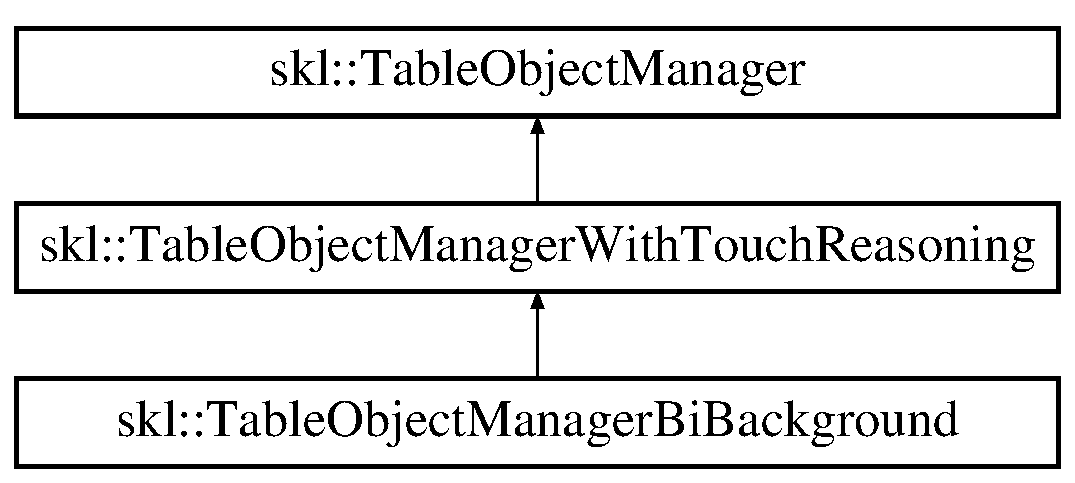
\includegraphics[height=3.000000cm]{classskl_1_1_table_object_manager_bi_background}
\end{center}
\end{figure}
\subsection*{Public Types}
\begin{DoxyCompactItemize}
\item 
\hypertarget{classskl_1_1_table_object_manager_bi_background_abe053e1676cc38136d416703f45e08b5}{}\label{classskl_1_1_table_object_manager_bi_background_abe053e1676cc38136d416703f45e08b5} 
typedef \hyperlink{classskl_1_1_filter_mat2_mat}{Filter\+Mat2\+Mat}$<$ size\+\_\+t $>$ {\bfseries Region\+Labeling\+Algorithm}
\item 
\hypertarget{classskl_1_1_table_object_manager_bi_background_a1576c40dbd074e438ad99a0eb4e3c519}{}\label{classskl_1_1_table_object_manager_bi_background_a1576c40dbd074e438ad99a0eb4e3c519} 
typedef \hyperlink{classskl_1_1_filter_mat2_mat}{Filter\+Mat2\+Mat}$<$ std\+::list$<$ size\+\_\+t $>$ $>$ {\bfseries Human\+Detector}
\end{DoxyCompactItemize}
\subsection*{Public Member Functions}
\begin{DoxyCompactItemize}
\item 
\hypertarget{classskl_1_1_table_object_manager_bi_background_a99f6f3daa03e567d324f27242a2a5440}{}\label{classskl_1_1_table_object_manager_bi_background_a99f6f3daa03e567d324f27242a2a5440} 
\hyperlink{classskl_1_1_table_object_manager_bi_background_a99f6f3daa03e567d324f27242a2a5440}{Table\+Object\+Manager\+Bi\+Background} (float \+\_\+\+\_\+learning\+\_\+rate=0.\+05, float \+\_\+\+\_\+learning\+\_\+rate2=0.\+05, cv\+::\+Ptr$<$ \hyperlink{classskl_1_1_background_subtract_algorithm}{Background\+Subtract\+Algorithm} $>$ bgs\+\_\+algo=new \hyperlink{classskl_1_1_tex_cut}{Tex\+Cut}(), cv\+::\+Ptr$<$ \hyperlink{classskl_1_1_filter_mat2_mat}{Region\+Labeling\+Algorithm} $>$ region\+\_\+labeling\+\_\+algo=new \hyperlink{classskl_1_1_region_labeling_simple}{Region\+Labeling\+Simple}(), cv\+::\+Ptr$<$ \hyperlink{classskl_1_1_filter_mat2_mat}{Human\+Detector} $>$ human\+\_\+detect\+\_\+algo=new \hyperlink{classskl_1_1_human_detector_workspace_end}{Human\+Detector\+Workspace\+End}(), cv\+::\+Ptr$<$ \hyperlink{classskl_1_1_filter_mat2_mat}{Region\+Labeling\+Algorithm} $>$ static\+\_\+region\+\_\+detect\+\_\+algo=new \hyperlink{classskl_1_1_static_region_detector}{Static\+Region\+Detector}(), cv\+::\+Ptr$<$ \hyperlink{classskl_1_1_filter_mat2_mat}{Region\+Labeling\+Algorithm} $>$ touched\+\_\+region\+\_\+detect\+\_\+algo=new \hyperlink{classskl_1_1_touched_region_detector}{Touched\+Region\+Detector}(), cv\+::\+Ptr$<$ \hyperlink{classskl_1_1_background_subtract_algorithm}{Background\+Subtract\+Algorithm} $>$ bgs\+\_\+algo2=new \hyperlink{classskl_1_1_tex_cut}{Tex\+Cut}(), cv\+::\+Ptr$<$ \hyperlink{classskl_1_1_patch_model_bi_background}{Patch\+Model\+Bi\+Background} $>$ patch\+\_\+model=new \hyperlink{classskl_1_1_patch_model_bi_background}{Patch\+Model\+Bi\+Background}())
\begin{DoxyCompactList}\small\item\em デフォルトコンストラクタ \end{DoxyCompactList}\item 
\hypertarget{classskl_1_1_table_object_manager_bi_background_aec0a2e4c54a2acdc20577fc849538f6b}{}\label{classskl_1_1_table_object_manager_bi_background_aec0a2e4c54a2acdc20577fc849538f6b} 
virtual \hyperlink{classskl_1_1_table_object_manager_bi_background_aec0a2e4c54a2acdc20577fc849538f6b}{$\sim$\+Table\+Object\+Manager\+Bi\+Background} ()
\begin{DoxyCompactList}\small\item\em デストラクタ \end{DoxyCompactList}\item 
\hypertarget{classskl_1_1_table_object_manager_bi_background_a0601f81ef37c34f1b6bd3c95fd9fbcf3}{}\label{classskl_1_1_table_object_manager_bi_background_a0601f81ef37c34f1b6bd3c95fd9fbcf3} 
virtual void {\bfseries compute} (const cv\+::\+Mat \&src, cv\+::\+Mat \&human, std\+::vector$<$ size\+\_\+t $>$ \&put\+\_\+objects, std\+::vector$<$ size\+\_\+t $>$ \&taken\+\_\+objects)
\item 
\hypertarget{classskl_1_1_table_object_manager_bi_background_a01c366c81705243ede4ce322089324c8}{}\label{classskl_1_1_table_object_manager_bi_background_a01c366c81705243ede4ce322089324c8} 
const cv\+::\+Mat \& {\bfseries bg2} () const
\end{DoxyCompactItemize}
\subsection*{Public Attributes}
\begin{DoxyCompactItemize}
\item 
\hypertarget{classskl_1_1_table_object_manager_bi_background_acf8fb57cd0bdd70f8aa8072b2417c809}{}\label{classskl_1_1_table_object_manager_bi_background_acf8fb57cd0bdd70f8aa8072b2417c809} 
float {\bfseries \+\_\+learning\+\_\+rate2}
\end{DoxyCompactItemize}
\subsection*{Protected Member Functions}
\begin{DoxyCompactItemize}
\item 
\hypertarget{classskl_1_1_table_object_manager_bi_background_a38c74ac192fce56a894e988906f16597}{}\label{classskl_1_1_table_object_manager_bi_background_a38c74ac192fce56a894e988906f16597} 
void {\bfseries bg\+\_\+subtract} (const cv\+::\+Mat \&src, cv\+::\+Mat \&dest)
\item 
\hypertarget{classskl_1_1_table_object_manager_bi_background_ad3587a9842be2f26376e535839503a8e}{}\label{classskl_1_1_table_object_manager_bi_background_ad3587a9842be2f26376e535839503a8e} 
void {\bfseries bg\+\_\+update} (const cv\+::\+Mat \&new\+\_\+bg, const cv\+::\+Mat \&update\+\_\+mask, const cv\+::\+Mat \&no\+\_\+touch\+\_\+fg)
\end{DoxyCompactItemize}
\subsection*{Protected Attributes}
\begin{DoxyCompactItemize}
\item 
\hypertarget{classskl_1_1_table_object_manager_bi_background_a630f4ad3a4c83b25c667cce5f4ee63aa}{}\label{classskl_1_1_table_object_manager_bi_background_a630f4ad3a4c83b25c667cce5f4ee63aa} 
cv\+::\+Mat {\bfseries \+\_\+bg2}
\item 
\hypertarget{classskl_1_1_table_object_manager_bi_background_a3797cfa1877c52118d44f37b5059e29c}{}\label{classskl_1_1_table_object_manager_bi_background_a3797cfa1877c52118d44f37b5059e29c} 
cv\+::\+Ptr$<$ \hyperlink{classskl_1_1_background_subtract_algorithm}{Background\+Subtract\+Algorithm} $>$ {\bfseries \+\_\+bgs\+\_\+algo2}
\item 
\hypertarget{classskl_1_1_table_object_manager_bi_background_aa75a91916b64a30ed728eca33da906a4}{}\label{classskl_1_1_table_object_manager_bi_background_aa75a91916b64a30ed728eca33da906a4} 
cv\+::\+Ptr$<$ \hyperlink{classskl_1_1_patch_model_bi_background}{Patch\+Model\+Bi\+Background} $>$ {\bfseries \+\_\+patch\+\_\+model\+\_\+ptr2}
\end{DoxyCompactItemize}
\subsection*{Additional Inherited Members}


\subsection{Detailed Description}
2つの背景を利用して背景差分を行いながら机上物体の出入りを管理するクラス 

The documentation for this class was generated from the following files\+:\begin{DoxyCompactItemize}
\item 
Open\+C\+V/include/\hyperlink{_table_object_manager_bi_background_8h}{Table\+Object\+Manager\+Bi\+Background.\+h}\item 
Open\+C\+V/src/Table\+Object\+Manager\+Bi\+Background.\+cpp\end{DoxyCompactItemize}

\hypertarget{classskl_1_1gpu_1_1_table_object_manager_bi_background}{}\section{skl\+:\+:gpu\+:\+:Table\+Object\+Manager\+Bi\+Background Class Reference}
\label{classskl_1_1gpu_1_1_table_object_manager_bi_background}\index{skl\+::gpu\+::\+Table\+Object\+Manager\+Bi\+Background@{skl\+::gpu\+::\+Table\+Object\+Manager\+Bi\+Background}}


2つの背景を利用して背景差分を行いながら机上物体の出入りを管理するクラス  




{\ttfamily \#include $<$Table\+Object\+Manager\+Bi\+Background\+Gpu.\+h$>$}

Inheritance diagram for skl\+:\+:gpu\+:\+:Table\+Object\+Manager\+Bi\+Background\+:\begin{figure}[H]
\begin{center}
\leavevmode
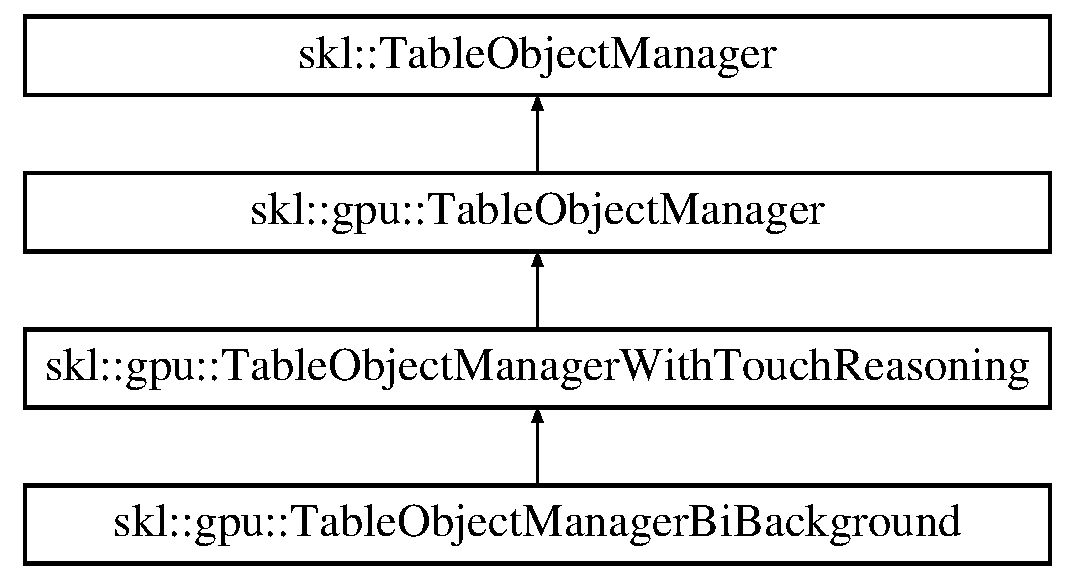
\includegraphics[height=4.000000cm]{classskl_1_1gpu_1_1_table_object_manager_bi_background}
\end{center}
\end{figure}
\subsection*{Public Types}
\begin{DoxyCompactItemize}
\item 
\hypertarget{classskl_1_1gpu_1_1_table_object_manager_bi_background_ab1cc00e9b9e4de283b2dd468b2a465ae}{}\label{classskl_1_1gpu_1_1_table_object_manager_bi_background_ab1cc00e9b9e4de283b2dd468b2a465ae} 
typedef \hyperlink{classskl_1_1_filter_mat2_mat}{Filter\+Mat2\+Mat}$<$ size\+\_\+t $>$ {\bfseries Region\+Labeling\+Algorithm}
\item 
\hypertarget{classskl_1_1gpu_1_1_table_object_manager_bi_background_a3f09b4d75c73ac8a41fe38789305a188}{}\label{classskl_1_1gpu_1_1_table_object_manager_bi_background_a3f09b4d75c73ac8a41fe38789305a188} 
typedef \hyperlink{classskl_1_1_filter_mat2_mat}{Filter\+Mat2\+Mat}$<$ std\+::list$<$ size\+\_\+t $>$ $>$ {\bfseries Human\+Detector}
\end{DoxyCompactItemize}
\subsection*{Public Member Functions}
\begin{DoxyCompactItemize}
\item 
\hypertarget{classskl_1_1gpu_1_1_table_object_manager_bi_background_a35b6b810cf8ef75b8be109f23907fd12}{}\label{classskl_1_1gpu_1_1_table_object_manager_bi_background_a35b6b810cf8ef75b8be109f23907fd12} 
{\bfseries Table\+Object\+Manager\+Bi\+Background} (float \+\_\+\+\_\+learning\+\_\+rate=0.\+05, float \+\_\+\+\_\+learning\+\_\+rate2=0.\+1, cv\+::\+Ptr$<$ \hyperlink{classskl_1_1gpu_1_1_tex_cut}{skl\+::gpu\+::\+Tex\+Cut} $>$ bgs\+\_\+algo=new \hyperlink{classskl_1_1gpu_1_1_tex_cut}{skl\+::gpu\+::\+Tex\+Cut}(), cv\+::\+Ptr$<$ \hyperlink{classskl_1_1_filter_mat2_mat}{Region\+Labeling\+Algorithm} $>$ region\+\_\+labeling\+\_\+algo=new \hyperlink{classskl_1_1_region_labeling_simple}{Region\+Labeling\+Simple}(), cv\+::\+Ptr$<$ \hyperlink{classskl_1_1_filter_mat2_mat}{Human\+Detector} $>$ human\+\_\+detect\+\_\+algo=new \hyperlink{classskl_1_1_human_detector_workspace_end}{Human\+Detector\+Workspace\+End}(), cv\+::\+Ptr$<$ \hyperlink{classskl_1_1_filter_mat2_mat}{Region\+Labeling\+Algorithm} $>$ static\+\_\+region\+\_\+detect\+\_\+algo=new \hyperlink{classskl_1_1_static_region_detector}{Static\+Region\+Detector}(), cv\+::\+Ptr$<$ \hyperlink{classskl_1_1_filter_mat2_mat}{Region\+Labeling\+Algorithm} $>$ touched\+\_\+region\+\_\+detect\+\_\+algo=new \hyperlink{classskl_1_1_touched_region_detector}{Touched\+Region\+Detector}(), cv\+::\+Ptr$<$ \hyperlink{classskl_1_1gpu_1_1_tex_cut}{skl\+::gpu\+::\+Tex\+Cut} $>$ bgs\+\_\+algo2=new \hyperlink{classskl_1_1gpu_1_1_tex_cut}{skl\+::gpu\+::\+Tex\+Cut}(), cv\+::\+Ptr$<$ \hyperlink{classskl_1_1_patch_model_bi_background}{Patch\+Model\+Bi\+Background} $>$ patch\+\_\+model=new \hyperlink{classskl_1_1_patch_model_bi_background}{Patch\+Model\+Bi\+Background}())
\item 
\hypertarget{classskl_1_1gpu_1_1_table_object_manager_bi_background_aec0a2e4c54a2acdc20577fc849538f6b}{}\label{classskl_1_1gpu_1_1_table_object_manager_bi_background_aec0a2e4c54a2acdc20577fc849538f6b} 
virtual \hyperlink{classskl_1_1gpu_1_1_table_object_manager_bi_background_aec0a2e4c54a2acdc20577fc849538f6b}{$\sim$\+Table\+Object\+Manager\+Bi\+Background} ()
\begin{DoxyCompactList}\small\item\em デストラクタ \end{DoxyCompactList}\item 
\hypertarget{classskl_1_1gpu_1_1_table_object_manager_bi_background_af875fcfdae8a5dca77ca964311b48f51}{}\label{classskl_1_1gpu_1_1_table_object_manager_bi_background_af875fcfdae8a5dca77ca964311b48f51} 
void {\bfseries compute} (const cv\+::\+Mat \&src, const cv\+::gpu\+::\+Gpu\+Mat \&src\+\_\+gpu, cv\+::\+Mat \&human, std\+::vector$<$ size\+\_\+t $>$ \&put\+\_\+objects, std\+::vector$<$ size\+\_\+t $>$ \&taken\+\_\+objects)
\item 
\hypertarget{classskl_1_1gpu_1_1_table_object_manager_bi_background_aed8aee1288baea588f768638a63bcc78}{}\label{classskl_1_1gpu_1_1_table_object_manager_bi_background_aed8aee1288baea588f768638a63bcc78} 
float {\bfseries learning\+\_\+rate2} ()
\item 
\hypertarget{classskl_1_1gpu_1_1_table_object_manager_bi_background_a28a17c7fa031753bf2e822732cf0a342}{}\label{classskl_1_1gpu_1_1_table_object_manager_bi_background_a28a17c7fa031753bf2e822732cf0a342} 
void {\bfseries learning\+\_\+rate2} (float val)
\item 
\hypertarget{classskl_1_1gpu_1_1_table_object_manager_bi_background_a4e9f3260c15904870a4c10f92d3fcdc2}{}\label{classskl_1_1gpu_1_1_table_object_manager_bi_background_a4e9f3260c15904870a4c10f92d3fcdc2} 
const cv\+::\+Ptr$<$ \hyperlink{classskl_1_1gpu_1_1_tex_cut}{skl\+::gpu\+::\+Tex\+Cut} $>$ \& {\bfseries bgs\+\_\+algo2} () const
\item 
\hypertarget{classskl_1_1gpu_1_1_table_object_manager_bi_background_aade4b07c073b566b7ef79078cc73fb90}{}\label{classskl_1_1gpu_1_1_table_object_manager_bi_background_aade4b07c073b566b7ef79078cc73fb90} 
void {\bfseries bgs\+\_\+algo2} (const cv\+::\+Ptr$<$ \hyperlink{classskl_1_1gpu_1_1_tex_cut}{skl\+::gpu\+::\+Tex\+Cut} $>$ \&\+\_\+\+\_\+bgs\+\_\+algo2)
\item 
\hypertarget{classskl_1_1gpu_1_1_table_object_manager_bi_background_a56b0da50686913af3c87e9439275f623}{}\label{classskl_1_1gpu_1_1_table_object_manager_bi_background_a56b0da50686913af3c87e9439275f623} 
const cv\+::\+Mat \& {\bfseries bg2} () const
\item 
\hypertarget{classskl_1_1gpu_1_1_table_object_manager_bi_background_aba49b65c3192a0a587d584d00c635424}{}\label{classskl_1_1gpu_1_1_table_object_manager_bi_background_aba49b65c3192a0a587d584d00c635424} 
void {\bfseries bg2} (const cv\+::\+Mat \&\+\_\+\+\_\+bg2)
\item 
\hypertarget{classskl_1_1gpu_1_1_table_object_manager_bi_background_a5f0954a0268c4ab3822d22512684ecdc}{}\label{classskl_1_1gpu_1_1_table_object_manager_bi_background_a5f0954a0268c4ab3822d22512684ecdc} 
double $\ast$ {\bfseries time\+\_\+compute} ()
\item 
\hypertarget{classskl_1_1gpu_1_1_table_object_manager_bi_background_acc610e7b507cf93d136b39eeaeaec44a}{}\label{classskl_1_1gpu_1_1_table_object_manager_bi_background_acc610e7b507cf93d136b39eeaeaec44a} 
double $\ast$ {\bfseries time\+\_\+bg} ()
\end{DoxyCompactItemize}
\subsection*{Public Attributes}
\begin{DoxyCompactItemize}
\item 
\hypertarget{classskl_1_1gpu_1_1_table_object_manager_bi_background_a93f0c48a1761cf9e91bc0fc771007423}{}\label{classskl_1_1gpu_1_1_table_object_manager_bi_background_a93f0c48a1761cf9e91bc0fc771007423} 
double {\bfseries t\+\_\+bg\+\_\+subtract}
\item 
\hypertarget{classskl_1_1gpu_1_1_table_object_manager_bi_background_a46582d9e962e0108fb4d1752509cd6ad}{}\label{classskl_1_1gpu_1_1_table_object_manager_bi_background_a46582d9e962e0108fb4d1752509cd6ad} 
double {\bfseries t\+\_\+bg\+\_\+subtract\+\_\+compute}
\item 
\hypertarget{classskl_1_1gpu_1_1_table_object_manager_bi_background_a704ecd6b95a6a0d5b9e8892968114fbd}{}\label{classskl_1_1gpu_1_1_table_object_manager_bi_background_a704ecd6b95a6a0d5b9e8892968114fbd} 
double {\bfseries t\+\_\+patch}
\item 
\hypertarget{classskl_1_1gpu_1_1_table_object_manager_bi_background_aa0f7bc3fc4737a58d88972914c0d7864}{}\label{classskl_1_1gpu_1_1_table_object_manager_bi_background_aa0f7bc3fc4737a58d88972914c0d7864} 
double {\bfseries t\+\_\+mask}
\item 
\hypertarget{classskl_1_1gpu_1_1_table_object_manager_bi_background_a8303151dde3b9a9653d9f242eb510122}{}\label{classskl_1_1gpu_1_1_table_object_manager_bi_background_a8303151dde3b9a9653d9f242eb510122} 
double {\bfseries t\+\_\+bg\+\_\+update}
\item 
\hypertarget{classskl_1_1gpu_1_1_table_object_manager_bi_background_a4c68b7b6bde6cd9c148e2ad4a7cc9c29}{}\label{classskl_1_1gpu_1_1_table_object_manager_bi_background_a4c68b7b6bde6cd9c148e2ad4a7cc9c29} 
double {\bfseries t\+\_\+bg\+\_\+update\+\_\+parfor}
\end{DoxyCompactItemize}
\subsection*{Protected Member Functions}
\begin{DoxyCompactItemize}
\item 
\hypertarget{classskl_1_1gpu_1_1_table_object_manager_bi_background_a3c1c9ab864bfb738b4236abac621a540}{}\label{classskl_1_1gpu_1_1_table_object_manager_bi_background_a3c1c9ab864bfb738b4236abac621a540} 
void {\bfseries bg\+\_\+subtract} (const cv\+::gpu\+::\+Gpu\+Mat \&src, cv\+::\+Mat \&dest)
\item 
\hypertarget{classskl_1_1gpu_1_1_table_object_manager_bi_background_abcc41b7f4769d0c1e8f660c08c972380}{}\label{classskl_1_1gpu_1_1_table_object_manager_bi_background_abcc41b7f4769d0c1e8f660c08c972380} 
void {\bfseries bg\+\_\+update} (const cv\+::\+Mat \&new\+\_\+bg, const cv\+::\+Mat \&non\+\_\+update\+\_\+mask, const cv\+::\+Mat \&no\+\_\+touch\+\_\+fg)
\end{DoxyCompactItemize}
\subsection*{Protected Attributes}
\begin{DoxyCompactItemize}
\item 
\hypertarget{classskl_1_1gpu_1_1_table_object_manager_bi_background_acdea7a839910b0e1776ad4e35405c072}{}\label{classskl_1_1gpu_1_1_table_object_manager_bi_background_acdea7a839910b0e1776ad4e35405c072} 
cv\+::\+Mat {\bfseries \+\_\+bg2}
\item 
\hypertarget{classskl_1_1gpu_1_1_table_object_manager_bi_background_ae8d4390f84787dd6d4ef6437c2b0e839}{}\label{classskl_1_1gpu_1_1_table_object_manager_bi_background_ae8d4390f84787dd6d4ef6437c2b0e839} 
float {\bfseries \+\_\+learning\+\_\+rate2}
\item 
\hypertarget{classskl_1_1gpu_1_1_table_object_manager_bi_background_a93460f344b945e352e84032dcac7df35}{}\label{classskl_1_1gpu_1_1_table_object_manager_bi_background_a93460f344b945e352e84032dcac7df35} 
cv\+::\+Ptr$<$ \hyperlink{classskl_1_1gpu_1_1_tex_cut}{skl\+::gpu\+::\+Tex\+Cut} $>$ {\bfseries \+\_\+bgs\+\_\+algo2}
\item 
\hypertarget{classskl_1_1gpu_1_1_table_object_manager_bi_background_a5f06d36acedb4c9418e7ad648c6235c7}{}\label{classskl_1_1gpu_1_1_table_object_manager_bi_background_a5f06d36acedb4c9418e7ad648c6235c7} 
cv\+::\+Ptr$<$ \hyperlink{classskl_1_1_patch_model_bi_background}{Patch\+Model\+Bi\+Background} $>$ {\bfseries \+\_\+patch\+\_\+model\+\_\+ptr2}
\item 
\hypertarget{classskl_1_1gpu_1_1_table_object_manager_bi_background_a2b4ec62aba8ac187b4c0cb1879500cec}{}\label{classskl_1_1gpu_1_1_table_object_manager_bi_background_a2b4ec62aba8ac187b4c0cb1879500cec} 
cv\+::gpu\+::\+Gpu\+Mat {\bfseries bg\+\_\+for\+\_\+texcut2}
\item 
\hypertarget{classskl_1_1gpu_1_1_table_object_manager_bi_background_a6815a6a60f9ddeedfcf21c70a8734480}{}\label{classskl_1_1gpu_1_1_table_object_manager_bi_background_a6815a6a60f9ddeedfcf21c70a8734480} 
cv\+::gpu\+::\+Gpu\+Mat {\bfseries \+\_\+bgs\+\_\+algo\+\_\+compute\+\_\+result}
\item 
\hypertarget{classskl_1_1gpu_1_1_table_object_manager_bi_background_aab0f1b6fc6c377376ce6010507033cb9}{}\label{classskl_1_1gpu_1_1_table_object_manager_bi_background_aab0f1b6fc6c377376ce6010507033cb9} 
cv\+::gpu\+::\+Gpu\+Mat {\bfseries \+\_\+bgs\+\_\+algo2\+\_\+compute\+\_\+result}
\item 
\hypertarget{classskl_1_1gpu_1_1_table_object_manager_bi_background_abc1c269ab3a63615e7c99bc1a73d9dbd}{}\label{classskl_1_1gpu_1_1_table_object_manager_bi_background_abc1c269ab3a63615e7c99bc1a73d9dbd} 
cv\+::gpu\+::\+Gpu\+Mat {\bfseries \+\_\+bitwise\+\_\+and\+\_\+result}
\item 
\hypertarget{classskl_1_1gpu_1_1_table_object_manager_bi_background_a4356b991069ee2a14c881a7c6b1056eb}{}\label{classskl_1_1gpu_1_1_table_object_manager_bi_background_a4356b991069ee2a14c881a7c6b1056eb} 
cv\+::gpu\+::\+Stream {\bfseries \+\_\+bgs\+\_\+algo\+\_\+compute\+\_\+stream}
\item 
\hypertarget{classskl_1_1gpu_1_1_table_object_manager_bi_background_ade7991cfdb5440ad179e5a7aac81f4b6}{}\label{classskl_1_1gpu_1_1_table_object_manager_bi_background_ade7991cfdb5440ad179e5a7aac81f4b6} 
cv\+::gpu\+::\+Stream {\bfseries \+\_\+bgs\+\_\+algo2\+\_\+compute\+\_\+stream}
\item 
\hypertarget{classskl_1_1gpu_1_1_table_object_manager_bi_background_aad147098dd2c5a4f0fd8264371523a21}{}\label{classskl_1_1gpu_1_1_table_object_manager_bi_background_aad147098dd2c5a4f0fd8264371523a21} 
cv\+::gpu\+::\+Stream {\bfseries \+\_\+bitwise\+\_\+and\+\_\+stream}
\item 
\hypertarget{classskl_1_1gpu_1_1_table_object_manager_bi_background_a6f7b46a1287a4b649049aada7fb21833}{}\label{classskl_1_1gpu_1_1_table_object_manager_bi_background_a6f7b46a1287a4b649049aada7fb21833} 
cv\+::gpu\+::\+Cuda\+Mem {\bfseries \+\_\+page\+\_\+locked\+\_\+bg2}
\end{DoxyCompactItemize}
\subsection*{Additional Inherited Members}


\subsection{Detailed Description}
2つの背景を利用して背景差分を行いながら机上物体の出入りを管理するクラス 

The documentation for this class was generated from the following files\+:\begin{DoxyCompactItemize}
\item 
Open\+C\+V\+G\+P\+U/include/Table\+Object\+Manager\+Bi\+Background\+Gpu.\+h\item 
Open\+C\+V\+G\+P\+U/src/Table\+Object\+Manager\+Bi\+Background.\+cpp\end{DoxyCompactItemize}

\hypertarget{classskl_1_1gpu_1_1_table_object_manager_with_touch_reasoning}{}\section{skl\+:\+:gpu\+:\+:Table\+Object\+Manager\+With\+Touch\+Reasoning Class Reference}
\label{classskl_1_1gpu_1_1_table_object_manager_with_touch_reasoning}\index{skl\+::gpu\+::\+Table\+Object\+Manager\+With\+Touch\+Reasoning@{skl\+::gpu\+::\+Table\+Object\+Manager\+With\+Touch\+Reasoning}}
Inheritance diagram for skl\+:\+:gpu\+:\+:Table\+Object\+Manager\+With\+Touch\+Reasoning\+:\begin{figure}[H]
\begin{center}
\leavevmode
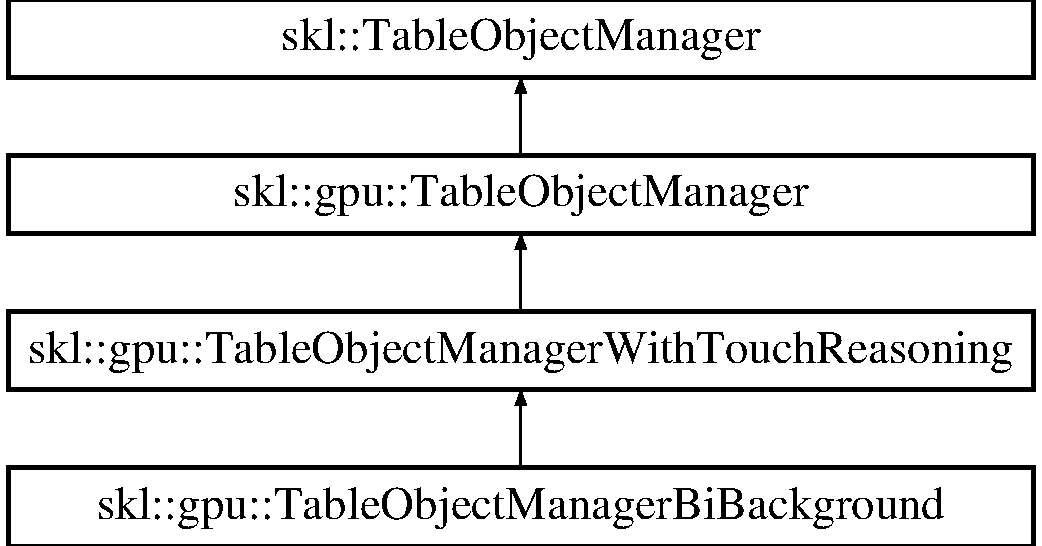
\includegraphics[height=4.000000cm]{classskl_1_1gpu_1_1_table_object_manager_with_touch_reasoning}
\end{center}
\end{figure}
\subsection*{Public Types}
\begin{DoxyCompactItemize}
\item 
\hypertarget{classskl_1_1gpu_1_1_table_object_manager_with_touch_reasoning_ad3124bcae3baed4b2e1da0f154e2d1d8}{}\label{classskl_1_1gpu_1_1_table_object_manager_with_touch_reasoning_ad3124bcae3baed4b2e1da0f154e2d1d8} 
typedef \hyperlink{classskl_1_1_filter_mat2_mat}{Filter\+Mat2\+Mat}$<$ size\+\_\+t $>$ {\bfseries Region\+Labeling\+Algorithm}
\item 
\hypertarget{classskl_1_1gpu_1_1_table_object_manager_with_touch_reasoning_a542b635e1260a1a1043c94aefffd2465}{}\label{classskl_1_1gpu_1_1_table_object_manager_with_touch_reasoning_a542b635e1260a1a1043c94aefffd2465} 
typedef \hyperlink{classskl_1_1_filter_mat2_mat}{Filter\+Mat2\+Mat}$<$ std\+::list$<$ size\+\_\+t $>$ $>$ {\bfseries Human\+Detector}
\end{DoxyCompactItemize}
\subsection*{Public Member Functions}
\begin{DoxyCompactItemize}
\item 
\hypertarget{classskl_1_1gpu_1_1_table_object_manager_with_touch_reasoning_a8d5dc605bb1cf199c16f77dbbd2a84fa}{}\label{classskl_1_1gpu_1_1_table_object_manager_with_touch_reasoning_a8d5dc605bb1cf199c16f77dbbd2a84fa} 
{\bfseries Table\+Object\+Manager\+With\+Touch\+Reasoning} (float \+\_\+\+\_\+learning\+\_\+rate=0.\+05, cv\+::\+Ptr$<$ \hyperlink{classskl_1_1gpu_1_1_tex_cut}{skl\+::gpu\+::\+Tex\+Cut} $>$ bgs\+\_\+algo=new \hyperlink{classskl_1_1gpu_1_1_tex_cut}{Tex\+Cut}(), cv\+::\+Ptr$<$ \hyperlink{classskl_1_1_filter_mat2_mat}{Region\+Labeling\+Algorithm} $>$ rl\+\_\+algo=new \hyperlink{classskl_1_1_region_labeling_simple}{Region\+Labeling\+Simple}(), cv\+::\+Ptr$<$ \hyperlink{classskl_1_1_filter_mat2_mat}{Human\+Detector} $>$ human\+\_\+detect\+\_\+algo=new \hyperlink{classskl_1_1_human_detector_workspace_end}{Human\+Detector\+Workspace\+End}(), cv\+::\+Ptr$<$ \hyperlink{classskl_1_1_filter_mat2_mat}{Region\+Labeling\+Algorithm} $>$ static\+\_\+region\+\_\+detect\+\_\+algo=new \hyperlink{classskl_1_1_static_region_detector}{Static\+Region\+Detector}(), cv\+::\+Ptr$<$ \hyperlink{classskl_1_1_filter_mat2_mat}{Region\+Labeling\+Algorithm} $>$ touched\+\_\+region\+\_\+detect\+\_\+algo=new \hyperlink{classskl_1_1_touched_region_detector}{Touched\+Region\+Detector}(), cv\+::\+Ptr$<$ \hyperlink{classskl_1_1_patch_model}{Patch\+Model} $>$ patch\+\_\+model=new \hyperlink{classskl_1_1_patch_model}{Patch\+Model}())
\item 
\hypertarget{classskl_1_1gpu_1_1_table_object_manager_with_touch_reasoning_a4d38c192d84e9184d11f2bbe55733e4f}{}\label{classskl_1_1gpu_1_1_table_object_manager_with_touch_reasoning_a4d38c192d84e9184d11f2bbe55733e4f} 
virtual \hyperlink{classskl_1_1gpu_1_1_table_object_manager_with_touch_reasoning_a4d38c192d84e9184d11f2bbe55733e4f}{$\sim$\+Table\+Object\+Manager\+With\+Touch\+Reasoning} ()
\begin{DoxyCompactList}\small\item\em デストラクタ \end{DoxyCompactList}\item 
\hypertarget{classskl_1_1gpu_1_1_table_object_manager_with_touch_reasoning_a7a82b7839390fe4d51cb5b572b4253c6}{}\label{classskl_1_1gpu_1_1_table_object_manager_with_touch_reasoning_a7a82b7839390fe4d51cb5b572b4253c6} 
void {\bfseries compute} (const cv\+::\+Mat \&src, const cv\+::gpu\+::\+Gpu\+Mat \&src\+\_\+gpu, cv\+::\+Mat \&human, std\+::vector$<$ size\+\_\+t $>$ \&put\+\_\+objects, std\+::vector$<$ size\+\_\+t $>$ \&taken\+\_\+objects)
\item 
\hypertarget{classskl_1_1gpu_1_1_table_object_manager_with_touch_reasoning_a406479505414e1ccb9f024d44a423202}{}\label{classskl_1_1gpu_1_1_table_object_manager_with_touch_reasoning_a406479505414e1ccb9f024d44a423202} 
const cv\+::\+Ptr$<$ \hyperlink{classskl_1_1_filter_mat2_mat}{Region\+Labeling\+Algorithm} $>$ \& {\bfseries trd\+\_\+algo} () const
\item 
\hypertarget{classskl_1_1gpu_1_1_table_object_manager_with_touch_reasoning_a829aa1a1edead8c607e176be17c5bbb4}{}\label{classskl_1_1gpu_1_1_table_object_manager_with_touch_reasoning_a829aa1a1edead8c607e176be17c5bbb4} 
void {\bfseries trd\+\_\+algo} (const cv\+::\+Ptr$<$ \hyperlink{classskl_1_1_filter_mat2_mat}{Region\+Labeling\+Algorithm} $>$ \&\+\_\+\+\_\+trd\+\_\+algo)
\end{DoxyCompactItemize}
\subsection*{Protected Attributes}
\begin{DoxyCompactItemize}
\item 
\hypertarget{classskl_1_1gpu_1_1_table_object_manager_with_touch_reasoning_ac2d437b86cd319442b00727cdc74ab49}{}\label{classskl_1_1gpu_1_1_table_object_manager_with_touch_reasoning_ac2d437b86cd319442b00727cdc74ab49} 
cv\+::\+Ptr$<$ \hyperlink{classskl_1_1_filter_mat2_mat}{Region\+Labeling\+Algorithm} $>$ {\bfseries \+\_\+trd\+\_\+algo}
\end{DoxyCompactItemize}
\subsection*{Additional Inherited Members}


The documentation for this class was generated from the following files\+:\begin{DoxyCompactItemize}
\item 
Open\+C\+V\+G\+P\+U/include/Table\+Object\+Manager\+With\+Touch\+Reasoning\+Gpu.\+h\item 
Open\+C\+V\+G\+P\+U/src/Table\+Object\+Manager\+With\+Touch\+Reasoning.\+cpp\end{DoxyCompactItemize}

\hypertarget{classskl_1_1_table_object_manager_with_touch_reasoning}{}\section{skl\+:\+:Table\+Object\+Manager\+With\+Touch\+Reasoning Class Reference}
\label{classskl_1_1_table_object_manager_with_touch_reasoning}\index{skl\+::\+Table\+Object\+Manager\+With\+Touch\+Reasoning@{skl\+::\+Table\+Object\+Manager\+With\+Touch\+Reasoning}}
Inheritance diagram for skl\+:\+:Table\+Object\+Manager\+With\+Touch\+Reasoning\+:\begin{figure}[H]
\begin{center}
\leavevmode
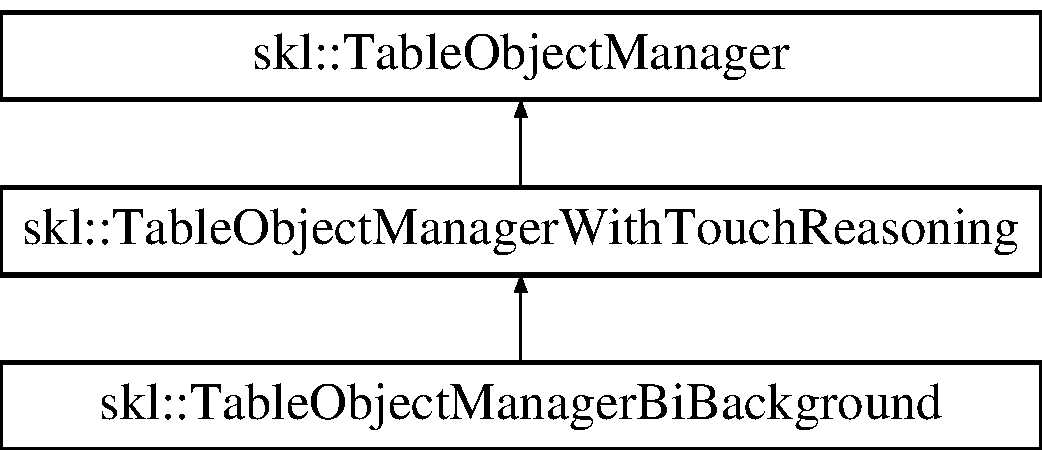
\includegraphics[height=3.000000cm]{classskl_1_1_table_object_manager_with_touch_reasoning}
\end{center}
\end{figure}
\subsection*{Public Types}
\begin{DoxyCompactItemize}
\item 
\hypertarget{classskl_1_1_table_object_manager_with_touch_reasoning_a3573af855f4889f4c2a8278450877766}{}\label{classskl_1_1_table_object_manager_with_touch_reasoning_a3573af855f4889f4c2a8278450877766} 
typedef \hyperlink{classskl_1_1_filter_mat2_mat}{Filter\+Mat2\+Mat}$<$ size\+\_\+t $>$ {\bfseries Region\+Labeling\+Algorithm}
\item 
\hypertarget{classskl_1_1_table_object_manager_with_touch_reasoning_a58a45db7b8f42581caf6ad84cb920a97}{}\label{classskl_1_1_table_object_manager_with_touch_reasoning_a58a45db7b8f42581caf6ad84cb920a97} 
typedef \hyperlink{classskl_1_1_filter_mat2_mat}{Filter\+Mat2\+Mat}$<$ std\+::list$<$ size\+\_\+t $>$ $>$ {\bfseries Human\+Detector}
\end{DoxyCompactItemize}
\subsection*{Public Member Functions}
\begin{DoxyCompactItemize}
\item 
\hypertarget{classskl_1_1_table_object_manager_with_touch_reasoning_afce161bd43896b8b274fc1b021b39a76}{}\label{classskl_1_1_table_object_manager_with_touch_reasoning_afce161bd43896b8b274fc1b021b39a76} 
\hyperlink{classskl_1_1_table_object_manager_with_touch_reasoning_afce161bd43896b8b274fc1b021b39a76}{Table\+Object\+Manager\+With\+Touch\+Reasoning} (float learning\+\_\+rate=0.\+05, cv\+::\+Ptr$<$ \hyperlink{classskl_1_1_background_subtract_algorithm}{Background\+Subtract\+Algorithm} $>$ background\+\_\+subtraction\+\_\+algo=new \hyperlink{classskl_1_1_tex_cut}{Tex\+Cut}(), cv\+::\+Ptr$<$ \hyperlink{classskl_1_1_filter_mat2_mat}{Region\+Labeling\+Algorithm} $>$ region\+\_\+labeling\+\_\+algo=new \hyperlink{classskl_1_1_region_labeling_simple}{Region\+Labeling\+Simple}(), cv\+::\+Ptr$<$ \hyperlink{classskl_1_1_filter_mat2_mat}{Human\+Detector} $>$ human\+\_\+detect\+\_\+algo=new \hyperlink{classskl_1_1_human_detector_workspace_end}{Human\+Detector\+Workspace\+End}(), cv\+::\+Ptr$<$ \hyperlink{classskl_1_1_filter_mat2_mat}{Region\+Labeling\+Algorithm} $>$ static\+\_\+region\+\_\+detect\+\_\+algo=new \hyperlink{classskl_1_1_static_region_detector}{Static\+Region\+Detector}(), cv\+::\+Ptr$<$ \hyperlink{classskl_1_1_filter_mat2_mat}{Region\+Labeling\+Algorithm} $>$ touched\+\_\+region\+\_\+detect\+\_\+algo=new \hyperlink{classskl_1_1_touched_region_detector}{Touched\+Region\+Detector}(), cv\+::\+Ptr$<$ \hyperlink{classskl_1_1_patch_model}{Patch\+Model} $>$ patch\+\_\+model=new \hyperlink{classskl_1_1_patch_model}{Patch\+Model}())
\begin{DoxyCompactList}\small\item\em デフォルトコンストラクタ \end{DoxyCompactList}\item 
\hypertarget{classskl_1_1_table_object_manager_with_touch_reasoning_a4d38c192d84e9184d11f2bbe55733e4f}{}\label{classskl_1_1_table_object_manager_with_touch_reasoning_a4d38c192d84e9184d11f2bbe55733e4f} 
virtual \hyperlink{classskl_1_1_table_object_manager_with_touch_reasoning_a4d38c192d84e9184d11f2bbe55733e4f}{$\sim$\+Table\+Object\+Manager\+With\+Touch\+Reasoning} ()
\begin{DoxyCompactList}\small\item\em デストラクタ \end{DoxyCompactList}\item 
\hypertarget{classskl_1_1_table_object_manager_with_touch_reasoning_ad7b5c7f0f6839cbf50a3b7cc94ad97f0}{}\label{classskl_1_1_table_object_manager_with_touch_reasoning_ad7b5c7f0f6839cbf50a3b7cc94ad97f0} 
void {\bfseries compute} (const cv\+::\+Mat \&src, cv\+::\+Mat \&human, std\+::vector$<$ size\+\_\+t $>$ \&put\+\_\+objects, std\+::vector$<$ size\+\_\+t $>$ \&taken\+\_\+objects)
\item 
\hypertarget{classskl_1_1_table_object_manager_with_touch_reasoning_a72f3c6f2f40fe9c21c8596acfc9c76ef}{}\label{classskl_1_1_table_object_manager_with_touch_reasoning_a72f3c6f2f40fe9c21c8596acfc9c76ef} 
const cv\+::\+Ptr$<$ \hyperlink{classskl_1_1_filter_mat2_mat}{Region\+Labeling\+Algorithm} $>$ \& {\bfseries trd\+\_\+algo} () const
\item 
\hypertarget{classskl_1_1_table_object_manager_with_touch_reasoning_aa73c7f50cf71adf18e4124bb2ed42806}{}\label{classskl_1_1_table_object_manager_with_touch_reasoning_aa73c7f50cf71adf18e4124bb2ed42806} 
void {\bfseries trd\+\_\+algo} (const cv\+::\+Ptr$<$ \hyperlink{classskl_1_1_filter_mat2_mat}{Region\+Labeling\+Algorithm} $>$ \&\+\_\+\+\_\+trd\+\_\+algo)
\end{DoxyCompactItemize}
\subsection*{Protected Attributes}
\begin{DoxyCompactItemize}
\item 
\hypertarget{classskl_1_1_table_object_manager_with_touch_reasoning_a5496bf298eb0c39c2447dfba5166e7cd}{}\label{classskl_1_1_table_object_manager_with_touch_reasoning_a5496bf298eb0c39c2447dfba5166e7cd} 
cv\+::\+Ptr$<$ \hyperlink{classskl_1_1_filter_mat2_mat}{Region\+Labeling\+Algorithm} $>$ {\bfseries \+\_\+trd\+\_\+algo}
\end{DoxyCompactItemize}
\subsection*{Additional Inherited Members}


The documentation for this class was generated from the following files\+:\begin{DoxyCompactItemize}
\item 
Open\+C\+V/include/\hyperlink{_table_object_manager_with_touch_reasoning_8h}{Table\+Object\+Manager\+With\+Touch\+Reasoning.\+h}\item 
Open\+C\+V/src/Table\+Object\+Manager\+With\+Touch\+Reasoning.\+cpp\end{DoxyCompactItemize}

\hypertarget{classskl_1_1_h_t_t_p_client_1_1tcp__client}{}\section{skl\+:\+:H\+T\+T\+P\+Client\+:\+:tcp\+\_\+client Class Reference}
\label{classskl_1_1_h_t_t_p_client_1_1tcp__client}\index{skl\+::\+H\+T\+T\+P\+Client\+::tcp\+\_\+client@{skl\+::\+H\+T\+T\+P\+Client\+::tcp\+\_\+client}}
\subsection*{Public Member Functions}
\begin{DoxyCompactItemize}
\item 
\hypertarget{classskl_1_1_h_t_t_p_client_1_1tcp__client_a24756c715e721929ec5a250e3a738886}{}\label{classskl_1_1_h_t_t_p_client_1_1tcp__client_a24756c715e721929ec5a250e3a738886} 
{\bfseries tcp\+\_\+client} (boost\+::asio\+::io\+\_\+service \&io\+\_\+service)
\item 
\hypertarget{classskl_1_1_h_t_t_p_client_1_1tcp__client_a38d63f5fcdfd44ca86a975438363654e}{}\label{classskl_1_1_h_t_t_p_client_1_1tcp__client_a38d63f5fcdfd44ca86a975438363654e} 
void {\bfseries write} (const std\+::string \&host, int port, boost\+::asio\+::streambuf $\ast$request)
\item 
\hypertarget{classskl_1_1_h_t_t_p_client_1_1tcp__client_ac7665658f03539b0d56dbcfb36d94a13}{}\label{classskl_1_1_h_t_t_p_client_1_1tcp__client_ac7665658f03539b0d56dbcfb36d94a13} 
unsigned int {\bfseries status\+\_\+code} () const
\item 
\hypertarget{classskl_1_1_h_t_t_p_client_1_1tcp__client_a81eb88228b5096dac26ca7eb93022eae}{}\label{classskl_1_1_h_t_t_p_client_1_1tcp__client_a81eb88228b5096dac26ca7eb93022eae} 
const std\+::string \& {\bfseries read} () const
\item 
\hypertarget{classskl_1_1_h_t_t_p_client_1_1tcp__client_a3b3944b46b557c6297c957754332bf06}{}\label{classskl_1_1_h_t_t_p_client_1_1tcp__client_a3b3944b46b557c6297c957754332bf06} 
const std\+::map$<$ std\+::string, std\+::string $>$ \& {\bfseries header} () const
\item 
\hypertarget{classskl_1_1_h_t_t_p_client_1_1tcp__client_a1ea561dea489534e3db958e970ef3156}{}\label{classskl_1_1_h_t_t_p_client_1_1tcp__client_a1ea561dea489534e3db958e970ef3156} 
boost\+::asio\+::io\+\_\+service \& {\bfseries io\+\_\+service} ()
\end{DoxyCompactItemize}
\subsection*{Protected Attributes}
\begin{DoxyCompactItemize}
\item 
\hypertarget{classskl_1_1_h_t_t_p_client_1_1tcp__client_a12201b0e55a829e8ab2b73b906ec04d4}{}\label{classskl_1_1_h_t_t_p_client_1_1tcp__client_a12201b0e55a829e8ab2b73b906ec04d4} 
std\+::map$<$ std\+::string, std\+::string $>$ {\bfseries header\+\_\+}
\end{DoxyCompactItemize}


The documentation for this class was generated from the following file\+:\begin{DoxyCompactItemize}
\item 
Core/include/\hyperlink{_h_t_t_p_client_8h}{H\+T\+T\+P\+Client.\+h}\end{DoxyCompactItemize}

\hypertarget{classskl_1_1_tex_cut}{}\section{skl\+:\+:Tex\+Cut Class Reference}
\label{classskl_1_1_tex_cut}\index{skl\+::\+Tex\+Cut@{skl\+::\+Tex\+Cut}}
Inheritance diagram for skl\+:\+:Tex\+Cut\+:\begin{figure}[H]
\begin{center}
\leavevmode
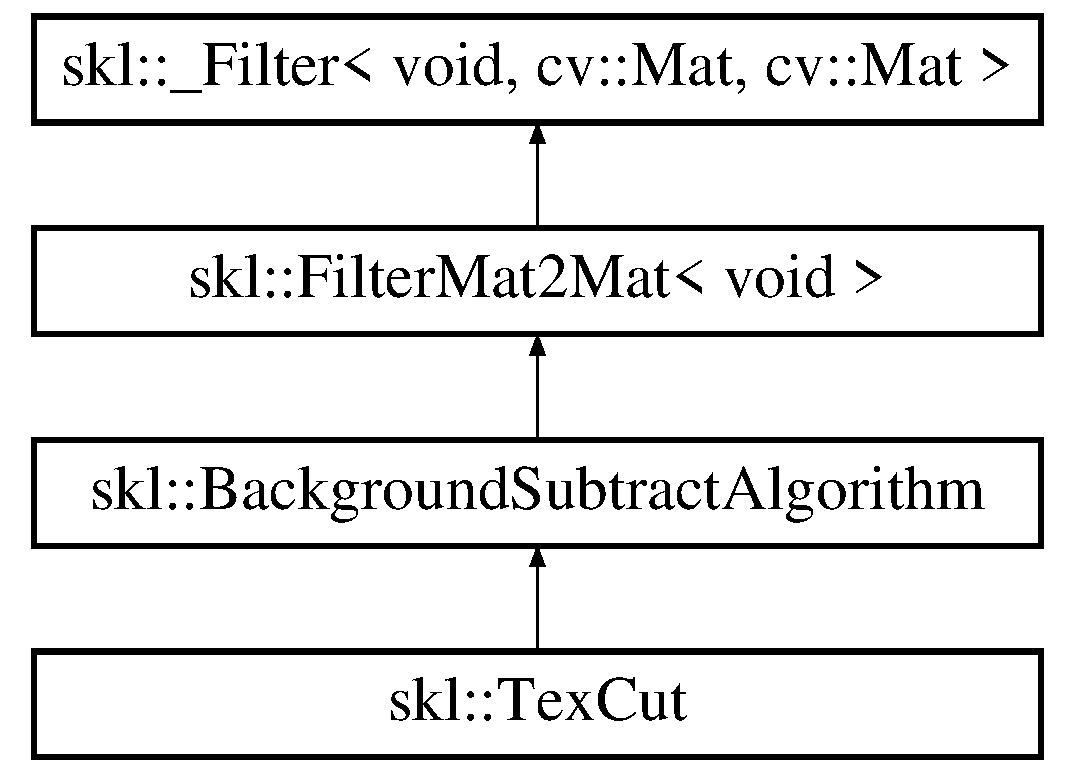
\includegraphics[height=4.000000cm]{classskl_1_1_tex_cut}
\end{center}
\end{figure}
\subsection*{Public Types}
\begin{DoxyCompactItemize}
\item 
\hypertarget{classskl_1_1_tex_cut_ab6e8259e8a77259adbc83a34a00f8a61}{}\label{classskl_1_1_tex_cut_ab6e8259e8a77259adbc83a34a00f8a61} 
typedef Graph$<$ int, int, int $>$ {\bfseries Tex\+Cut\+Graph}
\end{DoxyCompactItemize}
\subsection*{Public Member Functions}
\begin{DoxyCompactItemize}
\item 
\hypertarget{classskl_1_1_tex_cut_ab730801cda6ac254bf925fea10844e69}{}\label{classskl_1_1_tex_cut_ab730801cda6ac254bf925fea10844e69} 
{\bfseries Tex\+Cut} (float alpha=1.\+5, float smoothing\+\_\+term\+\_\+weight=1.\+0, float thresh\+\_\+tex\+\_\+diff=0.\+4, unsigned char over\+\_\+exposure\+\_\+thresh=248, unsigned char under\+\_\+exposure\+\_\+thresh=8, bool do\+Smoothing=true)
\item 
\hypertarget{classskl_1_1_tex_cut_a0aab9407bd5cf2a5d185ce3c42ccdf23}{}\label{classskl_1_1_tex_cut_a0aab9407bd5cf2a5d185ce3c42ccdf23} 
{\bfseries Tex\+Cut} (const cv\+::\+Mat \&bg1, const cv\+::\+Mat \&bg2, float alpha=1.\+0, float smoothing\+\_\+term\+\_\+weight=1.\+0, float thresh\+\_\+tex\+\_\+diff=0.\+4, unsigned char over\+\_\+exposure\+\_\+thresh=248, unsigned char under\+\_\+exposure\+\_\+thresh=8)
\item 
\hypertarget{classskl_1_1_tex_cut_afb6fbae7b1c1da054ab43107d8097263}{}\label{classskl_1_1_tex_cut_afb6fbae7b1c1da054ab43107d8097263} 
virtual void {\bfseries set\+Background} (const cv\+::\+Mat \&bg, bool no\+Smoothing=false)
\item 
\hypertarget{classskl_1_1_tex_cut_afbeb0cf8c109b9dd062a354b848ed86c}{}\label{classskl_1_1_tex_cut_afbeb0cf8c109b9dd062a354b848ed86c} 
void {\bfseries set\+Params} (float alpha=1.\+5, float smoothing\+\_\+term\+\_\+weight=1.\+5, float thresh\+\_\+tex\+\_\+diff=0.\+4, unsigned char over\+\_\+exposure\+\_\+thresh=248, unsigned char under\+\_\+exposure\+\_\+thresh=8)
\item 
\hypertarget{classskl_1_1_tex_cut_a1ad3f55b9aaede0b857a1c3f07397235}{}\label{classskl_1_1_tex_cut_a1ad3f55b9aaede0b857a1c3f07397235} 
void {\bfseries learn\+Image\+Noise\+Model} (const cv\+::\+Mat \&bg2)
\item 
\hypertarget{classskl_1_1_tex_cut_a13d0d07100c358dc72a44c3ed1cb41c0}{}\label{classskl_1_1_tex_cut_a13d0d07100c358dc72a44c3ed1cb41c0} 
void {\bfseries update\+Background\+Model} (const cv\+::\+Mat \&img)
\item 
\hypertarget{classskl_1_1_tex_cut_ada0f475c006b236325e201fcbb9dbbe4}{}\label{classskl_1_1_tex_cut_ada0f475c006b236325e201fcbb9dbbe4} 
cv\+::\+Mat {\bfseries background} () const
\item 
\hypertarget{classskl_1_1_tex_cut_a114d5710f0b2b6ba04c54f6a4df7f02f}{}\label{classskl_1_1_tex_cut_a114d5710f0b2b6ba04c54f6a4df7f02f} 
void {\bfseries set\+Noise\+Model} (const std\+::vector$<$ float $>$ \&noise\+\_\+std\+\_\+dev, const std\+::vector$<$ float $>$ \&gh\+\_\+expectation, const std\+::vector$<$ float $>$ \&gh\+\_\+std\+\_\+dev)
\item 
\hypertarget{classskl_1_1_tex_cut_a9e61e905d329f9f6333e7a95c249309f}{}\label{classskl_1_1_tex_cut_a9e61e905d329f9f6333e7a95c249309f} 
bool {\bfseries do\+Smoothing} () const
\item 
\hypertarget{classskl_1_1_tex_cut_aa51a66fef188c2570a5c4683087659b1}{}\label{classskl_1_1_tex_cut_aa51a66fef188c2570a5c4683087659b1} 
void {\bfseries do\+Smoothing} (bool \+\_\+\+\_\+do\+Smoothing)
\end{DoxyCompactItemize}
\subsection*{Protected Member Functions}
\begin{DoxyCompactItemize}
\item 
\hypertarget{classskl_1_1_tex_cut_a152906ca9a37972c1e9a80a9dc79093a}{}\label{classskl_1_1_tex_cut_a152906ca9a37972c1e9a80a9dc79093a} 
virtual void {\bfseries compute} (const cv\+::\+Mat \&src, const cv\+::\+Mat \&mask, cv\+::\+Mat \&dest)
\item 
\hypertarget{classskl_1_1_tex_cut_ae5f234d5a13fd3a9bbb24bf498b3ba5b}{}\label{classskl_1_1_tex_cut_ae5f234d5a13fd3a9bbb24bf498b3ba5b} 
void {\bfseries calc\+Edge\+Capacity} (const std\+::vector$<$ cv\+::\+Mat $>$ \&src, const std\+::vector$<$ cv\+::\+Mat $>$ \&sobel\+\_\+x, const std\+::vector$<$ cv\+::\+Mat $>$ \&sobel\+\_\+y, const std\+::vector$<$ cv\+::\+Mat $>$ \&bg\+\_\+img, const std\+::vector$<$ cv\+::\+Mat $>$ \&bg\+\_\+sobel\+\_\+x, const std\+::vector$<$ cv\+::\+Mat $>$ \&bg\+\_\+sobel\+\_\+y, const std\+::vector$<$ float $>$ \&noise\+\_\+std\+\_\+dev, const std\+::vector$<$ float $>$ \&gh\+\_\+expectation, const std\+::vector$<$ float $>$ \&gh\+\_\+std\+\_\+dev, float alpha, float smoothing\+\_\+term\+\_\+weight, float thresh\+\_\+tex\+\_\+diff, cv\+::\+Mat \&data\+\_\+term, cv\+::\+Mat \&smoothing\+\_\+term\+\_\+x, cv\+::\+Mat \&smoothing\+\_\+term\+\_\+y)
\item 
\hypertarget{classskl_1_1_tex_cut_a7bf838818a360db04e0eb97d6e1de769}{}\label{classskl_1_1_tex_cut_a7bf838818a360db04e0eb97d6e1de769} 
int {\bfseries calc\+Graph\+Cut} (const cv\+::\+Mat \&data\+\_\+term, const cv\+::\+Mat \&smoothing\+\_\+term\+\_\+x, const cv\+::\+Mat \&smoothing\+\_\+y)
\item 
\hypertarget{classskl_1_1_tex_cut_a9e2020aee23f54d8e2dcc259415959c4}{}\label{classskl_1_1_tex_cut_a9e2020aee23f54d8e2dcc259415959c4} 
void {\bfseries set\+Result} (const cv\+::\+Mat \&src, cv\+::\+Mat \&dest) const
\item 
\hypertarget{classskl_1_1_tex_cut_a204850a2ef37ed0a86d9b387f68cee40}{}\label{classskl_1_1_tex_cut_a204850a2ef37ed0a86d9b387f68cee40} 
void {\bfseries get\+Sobel} (const std\+::vector$<$ cv\+::\+Mat $>$ \&img, std\+::vector$<$ cv\+::\+Mat $>$ $\ast$sobel\+\_\+x, std\+::vector$<$ cv\+::\+Mat $>$ $\ast$sobel\+\_\+y)
\end{DoxyCompactItemize}
\subsection*{Protected Attributes}
\begin{DoxyCompactItemize}
\item 
\hypertarget{classskl_1_1_tex_cut_a009d4291f63514a949562a0ce0059a4a}{}\label{classskl_1_1_tex_cut_a009d4291f63514a949562a0ce0059a4a} 
bool {\bfseries \+\_\+do\+Smoothing}
\item 
\hypertarget{classskl_1_1_tex_cut_a3b56d571fda6b2aefa50f2d96b7bd4f3}{}\label{classskl_1_1_tex_cut_a3b56d571fda6b2aefa50f2d96b7bd4f3} 
std\+::vector$<$ cv\+::\+Mat $>$ {\bfseries bg\+\_\+img}
\item 
\hypertarget{classskl_1_1_tex_cut_a9f627c2647c654a98e308b29c8dc7976}{}\label{classskl_1_1_tex_cut_a9f627c2647c654a98e308b29c8dc7976} 
std\+::vector$<$ cv\+::\+Mat $>$ {\bfseries bg\+\_\+sobel\+\_\+x}
\item 
\hypertarget{classskl_1_1_tex_cut_a11d036175b39e40f324d9fdeaf92ab09}{}\label{classskl_1_1_tex_cut_a11d036175b39e40f324d9fdeaf92ab09} 
std\+::vector$<$ cv\+::\+Mat $>$ {\bfseries bg\+\_\+sobel\+\_\+y}
\item 
\hypertarget{classskl_1_1_tex_cut_ae6a696dbb5e396c06924c576d8f00916}{}\label{classskl_1_1_tex_cut_ae6a696dbb5e396c06924c576d8f00916} 
std\+::vector$<$ float $>$ {\bfseries noise\+\_\+std\+\_\+dev}
\item 
\hypertarget{classskl_1_1_tex_cut_a65520dd2b2cc7e6fdcee2df2b0b88544}{}\label{classskl_1_1_tex_cut_a65520dd2b2cc7e6fdcee2df2b0b88544} 
std\+::vector$<$ float $>$ {\bfseries gh\+\_\+expectation}
\item 
\hypertarget{classskl_1_1_tex_cut_a02e4bf3d27947c2b4fa4943deb6c4bdc}{}\label{classskl_1_1_tex_cut_a02e4bf3d27947c2b4fa4943deb6c4bdc} 
std\+::vector$<$ float $>$ {\bfseries gh\+\_\+std\+\_\+dev}
\item 
\hypertarget{classskl_1_1_tex_cut_a3c839d9fbfc31b39ed8746cbd843382c}{}\label{classskl_1_1_tex_cut_a3c839d9fbfc31b39ed8746cbd843382c} 
float {\bfseries alpha}
\item 
\hypertarget{classskl_1_1_tex_cut_ae560cca1682e51ce2a3b710ffc36393d}{}\label{classskl_1_1_tex_cut_ae560cca1682e51ce2a3b710ffc36393d} 
float {\bfseries smoothing\+\_\+term\+\_\+weight}
\item 
\hypertarget{classskl_1_1_tex_cut_a330f506ac8c577542a342882b17ea130}{}\label{classskl_1_1_tex_cut_a330f506ac8c577542a342882b17ea130} 
float {\bfseries thresh\+\_\+tex\+\_\+diff}
\item 
\hypertarget{classskl_1_1_tex_cut_ae224d178a3fd00cd5f1a0aaa13726878}{}\label{classskl_1_1_tex_cut_ae224d178a3fd00cd5f1a0aaa13726878} 
unsigned char {\bfseries over\+\_\+exposure\+\_\+thresh}
\item 
\hypertarget{classskl_1_1_tex_cut_ae07cb809d654962b87e56983b7368645}{}\label{classskl_1_1_tex_cut_ae07cb809d654962b87e56983b7368645} 
unsigned char {\bfseries under\+\_\+exposure\+\_\+thresh}
\item 
\hypertarget{classskl_1_1_tex_cut_abafc4ac9524a8bc0a1d9ab901890b70a}{}\label{classskl_1_1_tex_cut_abafc4ac9524a8bc0a1d9ab901890b70a} 
Tex\+Cut\+Graph $\ast$ {\bfseries g}
\item 
\hypertarget{classskl_1_1_tex_cut_a9db20e8dc253db61021acd1d1fdcd360}{}\label{classskl_1_1_tex_cut_a9db20e8dc253db61021acd1d1fdcd360} 
std\+::vector$<$ std\+::vector$<$ Tex\+Cut\+Graph\+::node\+\_\+id $>$ $>$ {\bfseries nodes}
\item 
\hypertarget{classskl_1_1_tex_cut_a8a7aa37cd4557825e6de41cf34185e43}{}\label{classskl_1_1_tex_cut_a8a7aa37cd4557825e6de41cf34185e43} 
cv\+::\+Mat {\bfseries \+\_\+background}
\end{DoxyCompactItemize}


The documentation for this class was generated from the following files\+:\begin{DoxyCompactItemize}
\item 
Open\+C\+V/include/Tex\+Cut.\+h\item 
Open\+C\+V/src/Tex\+Cut.\+cpp\end{DoxyCompactItemize}

\hypertarget{classskl_1_1gpu_1_1_tex_cut}{}\section{skl\+:\+:gpu\+:\+:Tex\+Cut Class Reference}
\label{classskl_1_1gpu_1_1_tex_cut}\index{skl\+::gpu\+::\+Tex\+Cut@{skl\+::gpu\+::\+Tex\+Cut}}


G\+P\+U上で\+Tex\+Cutによる背景差分を行うプログラム  




{\ttfamily \#include $<$Tex\+Cut.\+h$>$}

Inheritance diagram for skl\+:\+:gpu\+:\+:Tex\+Cut\+:\begin{figure}[H]
\begin{center}
\leavevmode
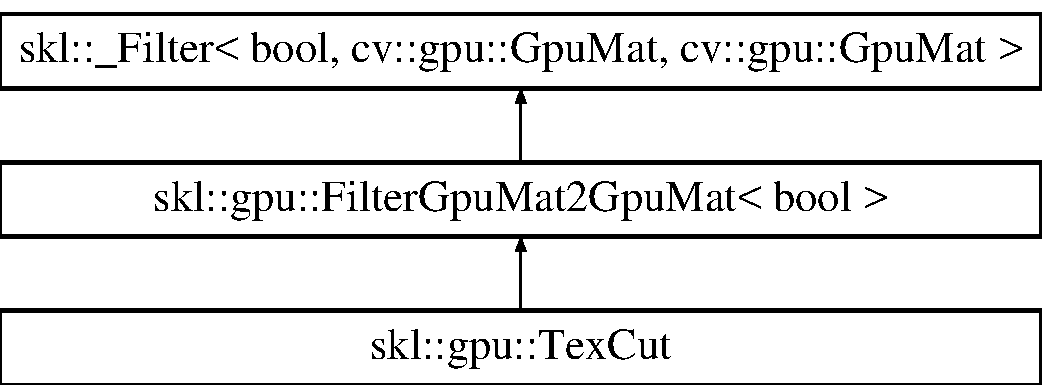
\includegraphics[height=3.000000cm]{classskl_1_1gpu_1_1_tex_cut}
\end{center}
\end{figure}
\subsection*{Public Member Functions}
\begin{DoxyCompactItemize}
\item 
\hypertarget{classskl_1_1gpu_1_1_tex_cut_a19ec5fb7b9020127cacee0def7bae3ed}{}\label{classskl_1_1gpu_1_1_tex_cut_a19ec5fb7b9020127cacee0def7bae3ed} 
\hyperlink{classskl_1_1gpu_1_1_tex_cut_a19ec5fb7b9020127cacee0def7bae3ed}{Tex\+Cut} (float alpha=1.\+5, float smoothing\+\_\+term\+\_\+weight=1.\+0, float thresh\+\_\+tex\+\_\+diff=0.\+4, unsigned char over\+\_\+exposure\+\_\+thresh=248, unsigned char under\+\_\+exposure\+\_\+thresh=8, bool do\+Smoothing=true)
\begin{DoxyCompactList}\small\item\em default constructor \end{DoxyCompactList}\item 
\hypertarget{classskl_1_1gpu_1_1_tex_cut_a04f718d5961299b4131879487494182c}{}\label{classskl_1_1gpu_1_1_tex_cut_a04f718d5961299b4131879487494182c} 
\hyperlink{classskl_1_1gpu_1_1_tex_cut_a04f718d5961299b4131879487494182c}{$\sim$\+Tex\+Cut} ()
\begin{DoxyCompactList}\small\item\em �ǥ��ȥ饯�� \end{DoxyCompactList}\item 
\hypertarget{classskl_1_1gpu_1_1_tex_cut_a77cbff21b38d5691de210f2d298fea01}{}\label{classskl_1_1gpu_1_1_tex_cut_a77cbff21b38d5691de210f2d298fea01} 
void {\bfseries set\+Params} (float alpha=1.\+5, float smoothing\+\_\+term\+\_\+weight=1.\+0, float thresh\+\_\+tex\+\_\+diff=0.\+4, unsigned char over\+\_\+exposure\+\_\+thresh=248, unsigned char under\+\_\+exposure\+\_\+thresh=8)
\item 
\hypertarget{classskl_1_1gpu_1_1_tex_cut_a8a3bac8170db78b4438c61dac1b811e0}{}\label{classskl_1_1gpu_1_1_tex_cut_a8a3bac8170db78b4438c61dac1b811e0} 
void {\bfseries set\+Noise\+Model} (const std\+::vector$<$ float $>$ \&noise\+\_\+std\+\_\+dev, const std\+::vector$<$ float $>$ \&gh\+\_\+expectation, const std\+::vector$<$ float $>$ \&gh\+\_\+std\+\_\+dev)
\item 
\hypertarget{classskl_1_1gpu_1_1_tex_cut_a9f17e1a9801b5c7fbeb8a18913077700}{}\label{classskl_1_1gpu_1_1_tex_cut_a9f17e1a9801b5c7fbeb8a18913077700} 
virtual bool {\bfseries compute} (const cv\+::gpu\+::\+Gpu\+Mat \&src, cv\+::gpu\+::\+Gpu\+Mat \&dest, cv\+::gpu\+::\+Stream \&stream\+\_\+external=cv\+::gpu\+::\+Stream\+::\+Null())
\item 
\hypertarget{classskl_1_1gpu_1_1_tex_cut_abb5cdf45b8994faf5189ec982bffce08}{}\label{classskl_1_1gpu_1_1_tex_cut_abb5cdf45b8994faf5189ec982bffce08} 
{\bfseries Tex\+Cut} (const cv\+::gpu\+::\+Gpu\+Mat \&bg1, const cv\+::gpu\+::\+Gpu\+Mat \&bg2, float alpha=1.\+0, float smoothing\+\_\+term\+\_\+weight=1.\+0, float thresh\+\_\+tex\+\_\+diff=0.\+4, unsigned char over\+\_\+exposure\+\_\+thresh=248, unsigned char under\+\_\+exposure\+\_\+thresh=8, bool do\+Smoothing=true)
\item 
\hypertarget{classskl_1_1gpu_1_1_tex_cut_a7a29872141520673771dfb60013e4aa0}{}\label{classskl_1_1gpu_1_1_tex_cut_a7a29872141520673771dfb60013e4aa0} 
void {\bfseries set\+Background} (const cv\+::gpu\+::\+Gpu\+Mat \&bg, bool no\+Smoothing=false)
\item 
\hypertarget{classskl_1_1gpu_1_1_tex_cut_a9bcc32ef68f1ab5352fa33ea909bd333}{}\label{classskl_1_1gpu_1_1_tex_cut_a9bcc32ef68f1ab5352fa33ea909bd333} 
void {\bfseries learn\+Image\+Noise\+Model} (const cv\+::gpu\+::\+Gpu\+Mat \&bg2)
\item 
\hypertarget{classskl_1_1gpu_1_1_tex_cut_a05adae108755609cfcdbeecca045ef9e}{}\label{classskl_1_1gpu_1_1_tex_cut_a05adae108755609cfcdbeecca045ef9e} 
void {\bfseries update\+Background\+Model} (const cv\+::gpu\+::\+Gpu\+Mat \&img)
\item 
\hypertarget{classskl_1_1gpu_1_1_tex_cut_a7da9b6a166f0d1bd87c63b77b722a6b1}{}\label{classskl_1_1gpu_1_1_tex_cut_a7da9b6a166f0d1bd87c63b77b722a6b1} 
void {\bfseries set\+Background} (const cv\+::\+Mat \&bg)
\item 
\hypertarget{classskl_1_1gpu_1_1_tex_cut_a1ecc86f3961f8febc70ad1b8f05a870d}{}\label{classskl_1_1gpu_1_1_tex_cut_a1ecc86f3961f8febc70ad1b8f05a870d} 
void {\bfseries learn\+Image\+Noise\+Model} (const cv\+::\+Mat \&bg2)
\item 
\hypertarget{classskl_1_1gpu_1_1_tex_cut_ac5dd4b7b756a6c354d8d9cb642babc0c}{}\label{classskl_1_1gpu_1_1_tex_cut_ac5dd4b7b756a6c354d8d9cb642babc0c} 
void {\bfseries update\+Background\+Model} (const cv\+::\+Mat \&img)
\item 
\hypertarget{classskl_1_1gpu_1_1_tex_cut_adc746bf324057c087feab95ef0982056}{}\label{classskl_1_1gpu_1_1_tex_cut_adc746bf324057c087feab95ef0982056} 
cv\+::\+Mat {\bfseries background} () const
\item 
\hypertarget{classskl_1_1gpu_1_1_tex_cut_a39564819fa2bbc56882e1a8dfc64209e}{}\label{classskl_1_1gpu_1_1_tex_cut_a39564819fa2bbc56882e1a8dfc64209e} 
bool {\bfseries do\+Smoothing} () const
\item 
\hypertarget{classskl_1_1gpu_1_1_tex_cut_a354d9d8c8509ce75bb15641159e65256}{}\label{classskl_1_1gpu_1_1_tex_cut_a354d9d8c8509ce75bb15641159e65256} 
void {\bfseries do\+Smoothing} (bool \+\_\+\+\_\+do\+Smoothing)
\item 
\hypertarget{classskl_1_1gpu_1_1_tex_cut_a6d2b4c631e685a5d873bacb85c90b190}{}\label{classskl_1_1gpu_1_1_tex_cut_a6d2b4c631e685a5d873bacb85c90b190} 
cv\+::gpu\+::\+Stream \& {\bfseries get\+Stream\+Set\+Background} (void)
\end{DoxyCompactItemize}
\subsection*{Public Attributes}
\begin{DoxyCompactItemize}
\item 
\hypertarget{classskl_1_1gpu_1_1_tex_cut_a720ccfa1a20523b6a8dd69dc55031d78}{}\label{classskl_1_1gpu_1_1_tex_cut_a720ccfa1a20523b6a8dd69dc55031d78} 
double $\ast$ {\bfseries t\+\_\+compute}
\item 
\hypertarget{classskl_1_1gpu_1_1_tex_cut_a6036f029093059ef33580ec3696d3498}{}\label{classskl_1_1gpu_1_1_tex_cut_a6036f029093059ef33580ec3696d3498} 
double {\bfseries t\+\_\+bg} \mbox{[}2\mbox{]}
\end{DoxyCompactItemize}
\subsection*{Protected Member Functions}
\begin{DoxyCompactItemize}
\item 
\hypertarget{classskl_1_1gpu_1_1_tex_cut_a84f0be67cf31aed4b3e885607314a330}{}\label{classskl_1_1gpu_1_1_tex_cut_a84f0be67cf31aed4b3e885607314a330} 
void {\bfseries alloc\+\_\+gpu} (const cv\+::\+Size \&img\+\_\+size, size\+\_\+t n\+Channels)
\end{DoxyCompactItemize}
\subsection*{Protected Attributes}
\begin{DoxyCompactItemize}
\item 
\hypertarget{classskl_1_1gpu_1_1_tex_cut_a8cfff71b4b342f808ec2bdb08938587c}{}\label{classskl_1_1gpu_1_1_tex_cut_a8cfff71b4b342f808ec2bdb08938587c} 
bool {\bfseries \+\_\+do\+Smoothing}
\item 
\hypertarget{classskl_1_1gpu_1_1_tex_cut_a14f856cabc0043857f11b47348b70610}{}\label{classskl_1_1gpu_1_1_tex_cut_a14f856cabc0043857f11b47348b70610} 
std\+::vector$<$ cv\+::gpu\+::\+Gpu\+Mat $>$ {\bfseries \+\_\+background}
\item 
\hypertarget{classskl_1_1gpu_1_1_tex_cut_afd8709d4020944511def0cffb595be71}{}\label{classskl_1_1gpu_1_1_tex_cut_afd8709d4020944511def0cffb595be71} 
std\+::vector$<$ cv\+::gpu\+::\+Gpu\+Mat $>$ {\bfseries \+\_\+bg\+\_\+blur\+\_\+temp}
\item 
\hypertarget{classskl_1_1gpu_1_1_tex_cut_a7a299cdf2a301a503839e0bced95f3e4}{}\label{classskl_1_1gpu_1_1_tex_cut_a7a299cdf2a301a503839e0bced95f3e4} 
std\+::vector$<$ cv\+::gpu\+::\+Gpu\+Mat $>$ {\bfseries \+\_\+bg\+\_\+sobel\+\_\+x}
\item 
\hypertarget{classskl_1_1gpu_1_1_tex_cut_a393b7f51df3f20d3cdcf53c6af3cc972}{}\label{classskl_1_1gpu_1_1_tex_cut_a393b7f51df3f20d3cdcf53c6af3cc972} 
std\+::vector$<$ cv\+::gpu\+::\+Gpu\+Mat $>$ {\bfseries \+\_\+bg\+\_\+sobel\+\_\+y}
\item 
\hypertarget{classskl_1_1gpu_1_1_tex_cut_aa6685ac7d607fb1cd97be316374a1e95}{}\label{classskl_1_1gpu_1_1_tex_cut_aa6685ac7d607fb1cd97be316374a1e95} 
cv\+::gpu\+::\+Gpu\+Mat {\bfseries \+\_\+bg\+\_\+buf\+\_\+sobel\+\_\+x}
\item 
\hypertarget{classskl_1_1gpu_1_1_tex_cut_a085ad3c00498843727e8742e16a668bb}{}\label{classskl_1_1gpu_1_1_tex_cut_a085ad3c00498843727e8742e16a668bb} 
cv\+::gpu\+::\+Gpu\+Mat {\bfseries \+\_\+bg\+\_\+buf\+\_\+sobel\+\_\+y}
\item 
\hypertarget{classskl_1_1gpu_1_1_tex_cut_a54f33c3c824d040d3c0cf706cbee7b5d}{}\label{classskl_1_1gpu_1_1_tex_cut_a54f33c3c824d040d3c0cf706cbee7b5d} 
std\+::vector$<$ cv\+::gpu\+::\+Gpu\+Mat $>$ {\bfseries \+\_\+bg\+\_\+tex\+\_\+intencity}
\item 
\hypertarget{classskl_1_1gpu_1_1_tex_cut_ad01e8a454af87f461621907622ae7c3c}{}\label{classskl_1_1gpu_1_1_tex_cut_ad01e8a454af87f461621907622ae7c3c} 
std\+::vector$<$ cv\+::gpu\+::\+Gpu\+Mat $>$ {\bfseries \+\_\+bg\+\_\+gradient\+\_\+heterogenuity}
\item 
\hypertarget{classskl_1_1gpu_1_1_tex_cut_aa661cd66555f522bff787aaca52c354b}{}\label{classskl_1_1gpu_1_1_tex_cut_aa661cd66555f522bff787aaca52c354b} 
std\+::vector$<$ float $>$ {\bfseries noise\+\_\+std\+\_\+dev}
\item 
\hypertarget{classskl_1_1gpu_1_1_tex_cut_a4813022abf9a9f4305f7b73527f6b514}{}\label{classskl_1_1gpu_1_1_tex_cut_a4813022abf9a9f4305f7b73527f6b514} 
std\+::vector$<$ float $>$ {\bfseries gh\+\_\+expectation}
\item 
\hypertarget{classskl_1_1gpu_1_1_tex_cut_ab741d9765e1899ab326795b940f6a618}{}\label{classskl_1_1gpu_1_1_tex_cut_ab741d9765e1899ab326795b940f6a618} 
std\+::vector$<$ float $>$ {\bfseries gh\+\_\+std\+\_\+dev}
\item 
\hypertarget{classskl_1_1gpu_1_1_tex_cut_a5600fc961ecda5a4527bfc4bdecc0d4b}{}\label{classskl_1_1gpu_1_1_tex_cut_a5600fc961ecda5a4527bfc4bdecc0d4b} 
float {\bfseries alpha}
\item 
\hypertarget{classskl_1_1gpu_1_1_tex_cut_a40fa380adc2ccd67a56219d3796e5b8d}{}\label{classskl_1_1gpu_1_1_tex_cut_a40fa380adc2ccd67a56219d3796e5b8d} 
float {\bfseries smoothing\+\_\+term\+\_\+weight}
\item 
\hypertarget{classskl_1_1gpu_1_1_tex_cut_aa7a35234ff57bb949ef19aac21830481}{}\label{classskl_1_1gpu_1_1_tex_cut_aa7a35234ff57bb949ef19aac21830481} 
float {\bfseries thresh\+\_\+tex\+\_\+diff}
\item 
\hypertarget{classskl_1_1gpu_1_1_tex_cut_ab48e26d5aa9049d6b9cd54f3fb155cef}{}\label{classskl_1_1gpu_1_1_tex_cut_ab48e26d5aa9049d6b9cd54f3fb155cef} 
unsigned char {\bfseries over\+\_\+exposure\+\_\+thresh}
\item 
\hypertarget{classskl_1_1gpu_1_1_tex_cut_ad21505b70952f3ff98185d9b188ece6e}{}\label{classskl_1_1gpu_1_1_tex_cut_ad21505b70952f3ff98185d9b188ece6e} 
unsigned char {\bfseries under\+\_\+exposure\+\_\+thresh}
\item 
\hypertarget{classskl_1_1gpu_1_1_tex_cut_ab8a34fbea50d34ada65866e9cad5cd4e}{}\label{classskl_1_1gpu_1_1_tex_cut_ab8a34fbea50d34ada65866e9cad5cd4e} 
cv\+::\+Size {\bfseries graph\+\_\+size}
\item 
\hypertarget{classskl_1_1gpu_1_1_tex_cut_a907def0c22b5f5b74d237054827947fa}{}\label{classskl_1_1gpu_1_1_tex_cut_a907def0c22b5f5b74d237054827947fa} 
cv\+::gpu\+::\+Gpu\+Mat {\bfseries terminals}
\item 
\hypertarget{classskl_1_1gpu_1_1_tex_cut_a21b3938b975bb21e22c700390bc0697b}{}\label{classskl_1_1gpu_1_1_tex_cut_a21b3938b975bb21e22c700390bc0697b} 
cv\+::gpu\+::\+Gpu\+Mat {\bfseries right\+Transp}
\item 
\hypertarget{classskl_1_1gpu_1_1_tex_cut_a50b9c7cb1cd48b7f0234a5fbdd34acf8}{}\label{classskl_1_1gpu_1_1_tex_cut_a50b9c7cb1cd48b7f0234a5fbdd34acf8} 
cv\+::gpu\+::\+Gpu\+Mat {\bfseries left\+Transp}
\item 
\hypertarget{classskl_1_1gpu_1_1_tex_cut_a8503ba5ccc4930542e8c038296d87ee2}{}\label{classskl_1_1gpu_1_1_tex_cut_a8503ba5ccc4930542e8c038296d87ee2} 
cv\+::gpu\+::\+Gpu\+Mat {\bfseries bottom}
\item 
\hypertarget{classskl_1_1gpu_1_1_tex_cut_a7ab4d9bf13da0ec674242b02b98c20b9}{}\label{classskl_1_1gpu_1_1_tex_cut_a7ab4d9bf13da0ec674242b02b98c20b9} 
cv\+::gpu\+::\+Gpu\+Mat {\bfseries top}
\item 
\hypertarget{classskl_1_1gpu_1_1_tex_cut_af4742375eb1b7e571a63c12c6cd0014d}{}\label{classskl_1_1gpu_1_1_tex_cut_af4742375eb1b7e571a63c12c6cd0014d} 
cv\+::gpu\+::\+Gpu\+Mat {\bfseries max\+\_\+intencity}
\item 
\hypertarget{classskl_1_1gpu_1_1_tex_cut_a924fd90150dd032ef30bf5e2f87a7322}{}\label{classskl_1_1gpu_1_1_tex_cut_a924fd90150dd032ef30bf5e2f87a7322} 
cv\+::gpu\+::\+Gpu\+Mat {\bfseries max\+\_\+gradient\+\_\+heterogenuity}
\item 
\hypertarget{classskl_1_1gpu_1_1_tex_cut_a7516fe05b68bd8616dd59c0bf7e315d6}{}\label{classskl_1_1gpu_1_1_tex_cut_a7516fe05b68bd8616dd59c0bf7e315d6} 
cv\+::gpu\+::\+Gpu\+Mat {\bfseries fg\+\_\+is\+\_\+over\+\_\+exposure}
\item 
\hypertarget{classskl_1_1gpu_1_1_tex_cut_ac4e23a172d72bc2a41871dc60ada9bba}{}\label{classskl_1_1gpu_1_1_tex_cut_ac4e23a172d72bc2a41871dc60ada9bba} 
cv\+::gpu\+::\+Gpu\+Mat {\bfseries fg\+\_\+is\+\_\+under\+\_\+exposure}
\item 
\hypertarget{classskl_1_1gpu_1_1_tex_cut_abee8e25ec391a878ca9a054665f81751}{}\label{classskl_1_1gpu_1_1_tex_cut_abee8e25ec391a878ca9a054665f81751} 
cv\+::gpu\+::\+Gpu\+Mat {\bfseries bg\+\_\+is\+\_\+over\+\_\+exposure}
\item 
\hypertarget{classskl_1_1gpu_1_1_tex_cut_acacd3700554f2cdee01512ec48833c9e}{}\label{classskl_1_1gpu_1_1_tex_cut_acacd3700554f2cdee01512ec48833c9e} 
cv\+::gpu\+::\+Gpu\+Mat {\bfseries bg\+\_\+is\+\_\+under\+\_\+exposure}
\item 
\hypertarget{classskl_1_1gpu_1_1_tex_cut_a8f8005dc8398031a8f01e3034a8470b6}{}\label{classskl_1_1gpu_1_1_tex_cut_a8f8005dc8398031a8f01e3034a8470b6} 
cv\+::gpu\+::\+Stream {\bfseries stream\+\_\+set\+Background}
\item 
\hypertarget{classskl_1_1gpu_1_1_tex_cut_a6d47a2588356abb2567a91368e857ec4}{}\label{classskl_1_1gpu_1_1_tex_cut_a6d47a2588356abb2567a91368e857ec4} 
\hyperlink{classskl_1_1_graphcut}{skl\+::\+Graphcut} {\bfseries gc\+\_\+algo}
\end{DoxyCompactItemize}


\subsection{Detailed Description}
G\+P\+U上で\+Tex\+Cutによる背景差分を行うプログラム 

The documentation for this class was generated from the following files\+:\begin{DoxyCompactItemize}
\item 
Open\+C\+V\+G\+P\+U/include/Tex\+Cut.\+h\item 
Open\+C\+V\+G\+P\+U/src/Tex\+Cut.\+cpp\end{DoxyCompactItemize}

\hypertarget{classskl_1_1_time}{}\section{skl\+:\+:Time Class Reference}
\label{classskl_1_1_time}\index{skl\+::\+Time@{skl\+::\+Time}}


\hyperlink{classskl_1_1_time}{Time}.  




{\ttfamily \#include $<$skl\+Time.\+h$>$}

Inheritance diagram for skl\+:\+:Time\+:\begin{figure}[H]
\begin{center}
\leavevmode
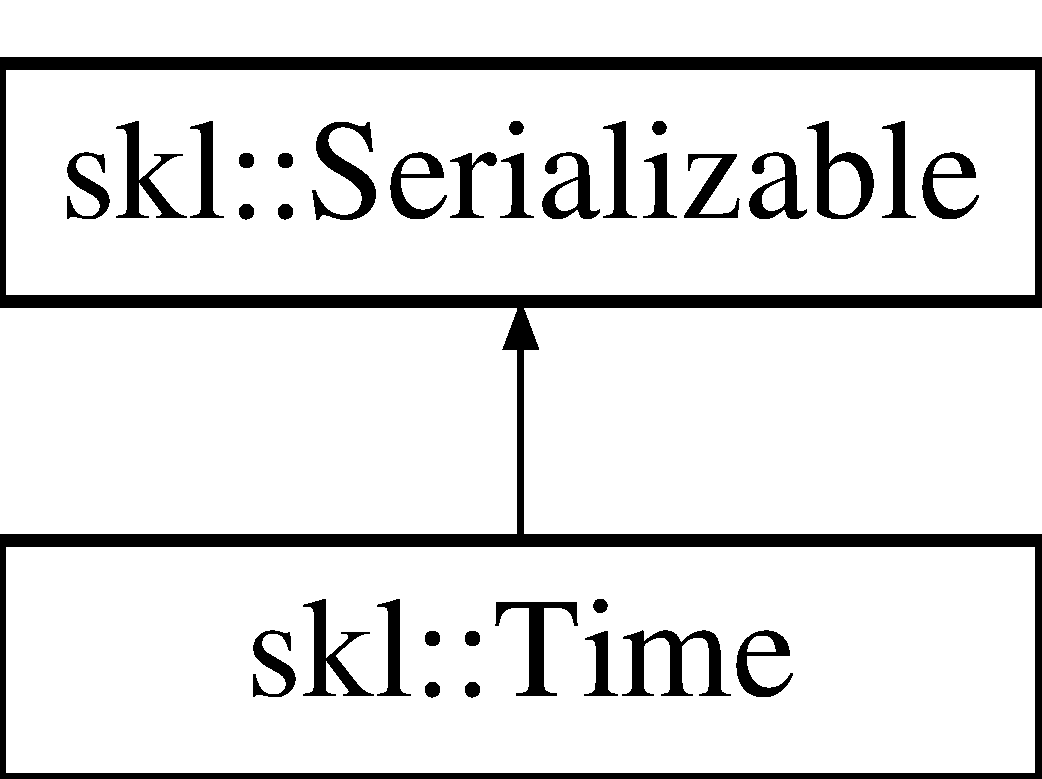
\includegraphics[height=2.000000cm]{classskl_1_1_time}
\end{center}
\end{figure}
\subsection*{Public Member Functions}
\begin{DoxyCompactItemize}
\item 
\hyperlink{classskl_1_1_time_acaa93bb22917f383bd74ea58ba1ae6e6}{Time} (long n\+Sec, int n\+M\+Sec, int n\+U\+Sec=0)
\begin{DoxyCompactList}\small\item\em コンストラクタ \end{DoxyCompactList}\item 
\hypertarget{classskl_1_1_time_a0408b1fdca0d7f086a8901e8594294bd}{}\label{classskl_1_1_time_a0408b1fdca0d7f086a8901e8594294bd} 
{\bfseries Time} (const \hyperlink{classskl_1_1_time}{Time} \&other)
\item 
\hypertarget{classskl_1_1_time_a48bd8879a40202da5d2186f463c1fde8}{}\label{classskl_1_1_time_a48bd8879a40202da5d2186f463c1fde8} 
{\bfseries Time} (int Y\+Y\+YY, int MM, int DD, int hh, int mm, int ss=0, int mmm=0, int usec=0)
\item 
\hypertarget{classskl_1_1_time_aa2ac2ed4b34fba1f6aadc09481601c77}{}\label{classskl_1_1_time_aa2ac2ed4b34fba1f6aadc09481601c77} 
\hyperlink{classskl_1_1_time}{Time} \& {\bfseries operator=} (const \hyperlink{classskl_1_1_time}{Time} \&other)
\item 
\hypertarget{classskl_1_1_time_aa4d8bd52002f3ca8bbbae51ebfdbc5ba}{}\label{classskl_1_1_time_aa4d8bd52002f3ca8bbbae51ebfdbc5ba} 
int {\bfseries get\+Year} () const
\item 
\hypertarget{classskl_1_1_time_ab7c2d4943a54151c9774a8bd704c3225}{}\label{classskl_1_1_time_ab7c2d4943a54151c9774a8bd704c3225} 
int {\bfseries get\+Month} () const
\item 
\hypertarget{classskl_1_1_time_af3982a0a799c7bf72483f837a1e1f799}{}\label{classskl_1_1_time_af3982a0a799c7bf72483f837a1e1f799} 
int {\bfseries get\+Day} () const
\item 
\hypertarget{classskl_1_1_time_a197e9349622b1daa36584b75e0642110}{}\label{classskl_1_1_time_a197e9349622b1daa36584b75e0642110} 
int {\bfseries get\+Hour} () const
\item 
\hypertarget{classskl_1_1_time_aecfe6ed53802a6db895473f6ddd514b0}{}\label{classskl_1_1_time_aecfe6ed53802a6db895473f6ddd514b0} 
int {\bfseries get\+Minute} () const
\item 
\hypertarget{classskl_1_1_time_a650a587f6499a627666d590b13dd3756}{}\label{classskl_1_1_time_a650a587f6499a627666d590b13dd3756} 
int {\bfseries get\+Second} () const
\item 
\hypertarget{classskl_1_1_time_a604e6a1d2ffb3fc3a81a269f891588fd}{}\label{classskl_1_1_time_a604e6a1d2ffb3fc3a81a269f891588fd} 
int {\bfseries get\+Milli\+Second} () const
\item 
void \hyperlink{classskl_1_1_time_aa4f63cd3ca5d31ef346b034af94da928}{parse\+String} (const std\+::string \&strxx)  throw (\+Time\+Format\+Exception)
\begin{DoxyCompactList}\small\item\em Default\+Formatterに従った文字列を解析し,値を得る \end{DoxyCompactList}\item 
std\+::string \hyperlink{classskl_1_1_time_affe013a77399e031ab79ab58ae9a306b}{to\+String} () const
\begin{DoxyCompactList}\small\item\em 文字列表現を返す \end{DoxyCompactList}\item 
void \hyperlink{classskl_1_1_time_acc9ee556bd8ddd2b85430b114892365f}{parse\+String} (const std\+::string \&str, \hyperlink{classskl_1_1_time_formatter}{Time\+Formatter} $\ast$timeformatter)  throw (\+Time\+Format\+Exception)
\begin{DoxyCompactList}\small\item\em 指定された\+Formatterを使って文字列を解析し,値を得る \end{DoxyCompactList}\item 
std\+::string \hyperlink{classskl_1_1_time_a44aed89659091d18d67e4503c47f0748}{to\+String} (\hyperlink{classskl_1_1_time_formatter}{Time\+Formatter} $\ast$timeformatter) const
\begin{DoxyCompactList}\small\item\em 指定された\+Formatterを使って文字列表現に変換する \end{DoxyCompactList}\item 
void \hyperlink{classskl_1_1_time_a523581fa6908222b9cec994dd325458c}{set\+Default\+Time\+Formatter} (const \hyperlink{classskl_1_1_time_formatter}{Time\+Formatter} $\ast$tf)
\begin{DoxyCompactList}\small\item\em デフォルトの\+Formatterを設定する. cloneされるので,引数で渡した\+Time\+Formatterオブジェクトは自分で解放すること. \end{DoxyCompactList}\item 
\hypertarget{classskl_1_1_time_a4ffada22c1d4786f68ba2c03689d948e}{}\label{classskl_1_1_time_a4ffada22c1d4786f68ba2c03689d948e} 
bool {\bfseries operator==} (const \hyperlink{classskl_1_1_time}{Time} \&other) const
\item 
\hypertarget{classskl_1_1_time_a28e4b688a730c859a25e0dea7548bddd}{}\label{classskl_1_1_time_a28e4b688a730c859a25e0dea7548bddd} 
bool {\bfseries operator!=} (const \hyperlink{classskl_1_1_time}{Time} \&other) const
\item 
\hypertarget{classskl_1_1_time_a21df0f8a7b08e71b3b04ccb2793d0aa4}{}\label{classskl_1_1_time_a21df0f8a7b08e71b3b04ccb2793d0aa4} 
bool {\bfseries operator$<$} (const \hyperlink{classskl_1_1_time}{Time} \&other) const
\item 
\hypertarget{classskl_1_1_time_a19eb5fa20b1e111cbe505eaaac4e407d}{}\label{classskl_1_1_time_a19eb5fa20b1e111cbe505eaaac4e407d} 
bool {\bfseries operator$>$} (const \hyperlink{classskl_1_1_time}{Time} \&other) const
\item 
\hypertarget{classskl_1_1_time_ae119912f5b9fbdc64b740100ed715b9e}{}\label{classskl_1_1_time_ae119912f5b9fbdc64b740100ed715b9e} 
bool {\bfseries operator$<$=} (const \hyperlink{classskl_1_1_time}{Time} \&other) const
\item 
\hypertarget{classskl_1_1_time_a88e8297465ed8c31909d37df3905f30a}{}\label{classskl_1_1_time_a88e8297465ed8c31909d37df3905f30a} 
bool {\bfseries operator$>$=} (const \hyperlink{classskl_1_1_time}{Time} \&other) const
\item 
\hypertarget{classskl_1_1_time_afbab90106944fd4b175d21418c418356}{}\label{classskl_1_1_time_afbab90106944fd4b175d21418c418356} 
long long {\bfseries operator-\/} (const \hyperlink{classskl_1_1_time}{Time} \&other) const
\item 
\hypertarget{classskl_1_1_time_acfeef5cfb9d63b959ceedfb59a1e9b24}{}\label{classskl_1_1_time_acfeef5cfb9d63b959ceedfb59a1e9b24} 
\hyperlink{classskl_1_1_time}{Time} {\bfseries operator+} (long long M\+Sec) const
\item 
\hypertarget{classskl_1_1_time_ac6b932ed1a3b61eb92f166167689be77}{}\label{classskl_1_1_time_ac6b932ed1a3b61eb92f166167689be77} 
\hyperlink{classskl_1_1_time}{Time} {\bfseries operator-\/} (long long M\+Sec) const
\item 
\hypertarget{classskl_1_1_time_ab4383eae5d09c10ea359d1caeec6f4b6}{}\label{classskl_1_1_time_ab4383eae5d09c10ea359d1caeec6f4b6} 
\hyperlink{classskl_1_1_time}{Time} \& {\bfseries operator+=} (long long M\+Sec)
\item 
\hypertarget{classskl_1_1_time_acfab25531e506af2831ac42a7d779b0b}{}\label{classskl_1_1_time_acfab25531e506af2831ac42a7d779b0b} 
\hyperlink{classskl_1_1_time}{Time} \& {\bfseries operator-\/=} (long long M\+Sec)
\item 
\hypertarget{classskl_1_1_time_a2b1f64ac04f08ec0516c99c402afed2a}{}\label{classskl_1_1_time_a2b1f64ac04f08ec0516c99c402afed2a} 
long long {\bfseries operator\%} (long long M\+Sec)
\item 
\hypertarget{classskl_1_1_time_ae6befd5d3f2ae2bca4f600860b2205a9}{}\label{classskl_1_1_time_ae6befd5d3f2ae2bca4f600860b2205a9} 
void {\bfseries print} (std\+::ostream \&out) const
\item 
\hypertarget{classskl_1_1_time_a49211f29831d4821318db5b45afb5bfe}{}\label{classskl_1_1_time_a49211f29831d4821318db5b45afb5bfe} 
long \hyperlink{classskl_1_1_time_a49211f29831d4821318db5b45afb5bfe}{\+\_\+buf\+\_\+size} () const
\begin{DoxyCompactList}\small\item\em \+\_\+serializeで生成される予定のbufの長さを返す \end{DoxyCompactList}\item 
\hypertarget{classskl_1_1_time_ae251fce04eb6c0d5181485b2393b3273}{}\label{classskl_1_1_time_ae251fce04eb6c0d5181485b2393b3273} 
void \hyperlink{classskl_1_1_time_ae251fce04eb6c0d5181485b2393b3273}{\+\_\+serialize} ()
\begin{DoxyCompactList}\small\item\em クラスの中身を直列化してメンバ変数のbufに格納する \end{DoxyCompactList}\item 
\hypertarget{classskl_1_1_time_a62573da15db11ef9379b7b113c972ab6}{}\label{classskl_1_1_time_a62573da15db11ef9379b7b113c972ab6} 
void \hyperlink{classskl_1_1_time_a62573da15db11ef9379b7b113c972ab6}{\+\_\+deserialize} (const char $\ast$\hyperlink{classskl_1_1_serializable_a1d203d9f0049ce37183a0dcefbc6399a}{buf}, long \hyperlink{classskl_1_1_serializable_a087eb19fada917a42b8411bfecbac0f1}{buf\+\_\+size})
\begin{DoxyCompactList}\small\item\em 直列化されたクラスの中身を読み込む \end{DoxyCompactList}\end{DoxyCompactItemize}
\subsection*{Static Public Member Functions}
\begin{DoxyCompactItemize}
\item 
static \hyperlink{classskl_1_1_time}{Time} \hyperlink{classskl_1_1_time_a017b1cdbe2841f1b7f4c9323e3cac184}{now} (int utc\+\_\+local\+\_\+diff=J\+P\+\_\+\+L\+O\+C\+AL)
\begin{DoxyCompactList}\small\item\em 現在時刻を表すオブジェクトを返す静的メソッド \end{DoxyCompactList}\end{DoxyCompactItemize}
\subsection*{Static Public Attributes}
\begin{DoxyCompactItemize}
\item 
\hypertarget{classskl_1_1_time_a252caab991847ae076f51597fcd3966b}{}\label{classskl_1_1_time_a252caab991847ae076f51597fcd3966b} 
static int {\bfseries J\+P\+\_\+\+L\+O\+C\+AL} = 9
\end{DoxyCompactItemize}
\subsection*{Additional Inherited Members}


\subsection{Detailed Description}
\hyperlink{classskl_1_1_time}{Time}. 

非負で1usec単位のタイムスタンプを扱えるクラス 

\subsection{Constructor \& Destructor Documentation}
\hypertarget{classskl_1_1_time_acaa93bb22917f383bd74ea58ba1ae6e6}{}\label{classskl_1_1_time_acaa93bb22917f383bd74ea58ba1ae6e6} 
\index{skl\+::\+Time@{skl\+::\+Time}!Time@{Time}}
\index{Time@{Time}!skl\+::\+Time@{skl\+::\+Time}}
\subsubsection{\texorpdfstring{Time()}{Time()}}
{\footnotesize\ttfamily skl\+::\+Time\+::\+Time (\begin{DoxyParamCaption}\item[{long}]{n\+Sec,  }\item[{int}]{n\+M\+Sec,  }\item[{int}]{n\+U\+Sec = {\ttfamily 0} }\end{DoxyParamCaption})}



コンストラクタ 


\begin{DoxyParams}{Parameters}
{\em n\+Sec} & 紀元(1970年1月1日00\+:00\+:00 U\+TC)からの経過時間 Second \\
\hline
{\em n\+M\+Sec} & Mili\+Second 3桁 \\
\hline
{\em n\+U\+Sec} & Micro\+Second 3桁 \\
\hline
\end{DoxyParams}


\subsection{Member Function Documentation}
\hypertarget{classskl_1_1_time_a017b1cdbe2841f1b7f4c9323e3cac184}{}\label{classskl_1_1_time_a017b1cdbe2841f1b7f4c9323e3cac184} 
\index{skl\+::\+Time@{skl\+::\+Time}!now@{now}}
\index{now@{now}!skl\+::\+Time@{skl\+::\+Time}}
\subsubsection{\texorpdfstring{now()}{now()}}
{\footnotesize\ttfamily static \hyperlink{classskl_1_1_time}{Time} skl\+::\+Time\+::now (\begin{DoxyParamCaption}\item[{int}]{utc\+\_\+local\+\_\+diff = {\ttfamily JP\+\_\+LOCAL} }\end{DoxyParamCaption})\hspace{0.3cm}{\ttfamily [inline]}, {\ttfamily [static]}}



現在時刻を表すオブジェクトを返す静的メソッド 

\begin{DoxyReturn}{Returns}
現在時刻を表す \hyperlink{classskl_1_1_time}{Time} オブジェクト 
\end{DoxyReturn}
\hypertarget{classskl_1_1_time_aa4f63cd3ca5d31ef346b034af94da928}{}\label{classskl_1_1_time_aa4f63cd3ca5d31ef346b034af94da928} 
\index{skl\+::\+Time@{skl\+::\+Time}!parse\+String@{parse\+String}}
\index{parse\+String@{parse\+String}!skl\+::\+Time@{skl\+::\+Time}}
\subsubsection{\texorpdfstring{parse\+String()}{parseString()}\hspace{0.1cm}{\footnotesize\ttfamily [1/2]}}
{\footnotesize\ttfamily void skl\+::\+Time\+::parse\+String (\begin{DoxyParamCaption}\item[{const std\+::string \&}]{str }\end{DoxyParamCaption}) throw  \hyperlink{classskl_1_1_time_format_exception}{Time\+Format\+Exception}) }



Default\+Formatterに従った文字列を解析し,値を得る 


\begin{DoxyParams}{Parameters}
{\em str} & 変換元の文字列 \\
\hline
\end{DoxyParams}
\hypertarget{classskl_1_1_time_acc9ee556bd8ddd2b85430b114892365f}{}\label{classskl_1_1_time_acc9ee556bd8ddd2b85430b114892365f} 
\index{skl\+::\+Time@{skl\+::\+Time}!parse\+String@{parse\+String}}
\index{parse\+String@{parse\+String}!skl\+::\+Time@{skl\+::\+Time}}
\subsubsection{\texorpdfstring{parse\+String()}{parseString()}\hspace{0.1cm}{\footnotesize\ttfamily [2/2]}}
{\footnotesize\ttfamily void skl\+::\+Time\+::parse\+String (\begin{DoxyParamCaption}\item[{const std\+::string \&}]{str,  }\item[{\hyperlink{classskl_1_1_time_formatter}{Time\+Formatter} $\ast$}]{timeformatter }\end{DoxyParamCaption}) throw  \hyperlink{classskl_1_1_time_format_exception}{Time\+Format\+Exception}) }



指定された\+Formatterを使って文字列を解析し,値を得る 


\begin{DoxyParams}{Parameters}
{\em str} & 指定された\+Formatterに従った文字列 \\
\hline
{\em timeformatter} & Formatter \\
\hline
\end{DoxyParams}
\hypertarget{classskl_1_1_time_a523581fa6908222b9cec994dd325458c}{}\label{classskl_1_1_time_a523581fa6908222b9cec994dd325458c} 
\index{skl\+::\+Time@{skl\+::\+Time}!set\+Default\+Time\+Formatter@{set\+Default\+Time\+Formatter}}
\index{set\+Default\+Time\+Formatter@{set\+Default\+Time\+Formatter}!skl\+::\+Time@{skl\+::\+Time}}
\subsubsection{\texorpdfstring{set\+Default\+Time\+Formatter()}{setDefaultTimeFormatter()}}
{\footnotesize\ttfamily void skl\+::\+Time\+::set\+Default\+Time\+Formatter (\begin{DoxyParamCaption}\item[{const \hyperlink{classskl_1_1_time_formatter}{Time\+Formatter} $\ast$}]{tf }\end{DoxyParamCaption})}



デフォルトの\+Formatterを設定する. cloneされるので,引数で渡した\+Time\+Formatterオブジェクトは自分で解放すること. 


\begin{DoxyParams}{Parameters}
{\em tf} & 指定したい\+Time\+Formatter \\
\hline
\end{DoxyParams}
\hypertarget{classskl_1_1_time_affe013a77399e031ab79ab58ae9a306b}{}\label{classskl_1_1_time_affe013a77399e031ab79ab58ae9a306b} 
\index{skl\+::\+Time@{skl\+::\+Time}!to\+String@{to\+String}}
\index{to\+String@{to\+String}!skl\+::\+Time@{skl\+::\+Time}}
\subsubsection{\texorpdfstring{to\+String()}{toString()}\hspace{0.1cm}{\footnotesize\ttfamily [1/2]}}
{\footnotesize\ttfamily std\+::string skl\+::\+Time\+::to\+String (\begin{DoxyParamCaption}{ }\end{DoxyParamCaption}) const}



文字列表現を返す 

\begin{DoxyReturn}{Returns}
Default\+Formatterに従って変換した文字列 
\end{DoxyReturn}
\hypertarget{classskl_1_1_time_a44aed89659091d18d67e4503c47f0748}{}\label{classskl_1_1_time_a44aed89659091d18d67e4503c47f0748} 
\index{skl\+::\+Time@{skl\+::\+Time}!to\+String@{to\+String}}
\index{to\+String@{to\+String}!skl\+::\+Time@{skl\+::\+Time}}
\subsubsection{\texorpdfstring{to\+String()}{toString()}\hspace{0.1cm}{\footnotesize\ttfamily [2/2]}}
{\footnotesize\ttfamily std\+::string skl\+::\+Time\+::to\+String (\begin{DoxyParamCaption}\item[{\hyperlink{classskl_1_1_time_formatter}{Time\+Formatter} $\ast$}]{timeformatter }\end{DoxyParamCaption}) const}



指定された\+Formatterを使って文字列表現に変換する 


\begin{DoxyParams}{Parameters}
{\em timeformatter} & Formatter\\
\hline
\end{DoxyParams}
\begin{DoxyReturn}{Returns}
このオブジェクトの文字列表現 
\end{DoxyReturn}


The documentation for this class was generated from the following files\+:\begin{DoxyCompactItemize}
\item 
Core/include/skl\+Time.\+h\item 
Core/src/skl\+Time.\+cpp\end{DoxyCompactItemize}

\hypertarget{classskl_1_1_time_format_exception}{}\section{skl\+:\+:Time\+Format\+Exception Class Reference}
\label{classskl_1_1_time_format_exception}\index{skl\+::\+Time\+Format\+Exception@{skl\+::\+Time\+Format\+Exception}}


\hyperlink{classskl_1_1_time_format_exception}{Time\+Format\+Exception}.  




{\ttfamily \#include $<$Time\+Format\+Exception.\+h$>$}

Inheritance diagram for skl\+:\+:Time\+Format\+Exception\+:\begin{figure}[H]
\begin{center}
\leavevmode
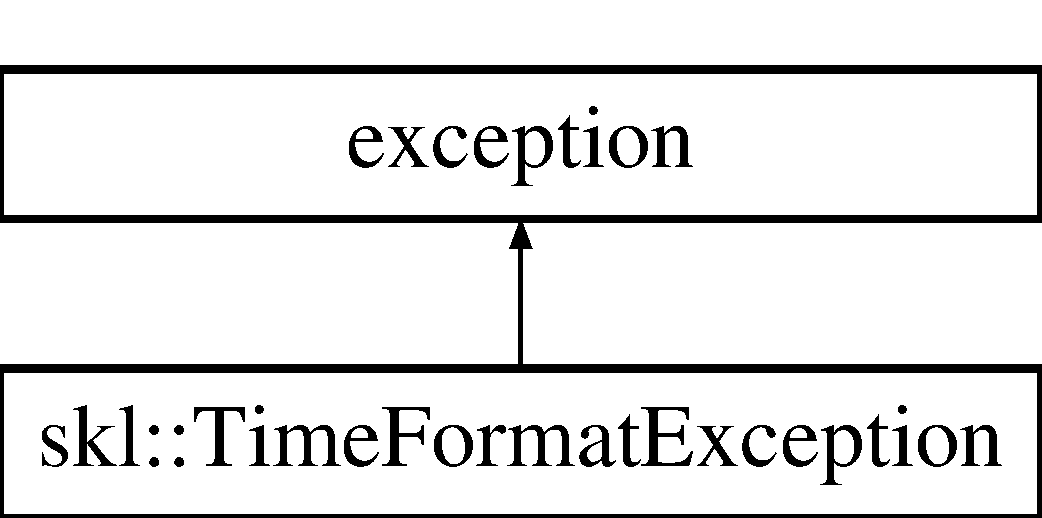
\includegraphics[height=2.000000cm]{classskl_1_1_time_format_exception}
\end{center}
\end{figure}
\subsection*{Public Member Functions}
\begin{DoxyCompactItemize}
\item 
\hypertarget{classskl_1_1_time_format_exception_a5704eda6974105a00e17437ca3b2fa0d}{}\label{classskl_1_1_time_format_exception_a5704eda6974105a00e17437ca3b2fa0d} 
virtual \hyperlink{classskl_1_1_time_format_exception_a5704eda6974105a00e17437ca3b2fa0d}{$\sim$\+Time\+Format\+Exception} ()  throw ()
\begin{DoxyCompactList}\small\item\em デストラクタ \end{DoxyCompactList}\item 
\hyperlink{classskl_1_1_time_format_exception_ae2d980f18722c3b6e209f0abd36a427f}{Time\+Format\+Exception} (const std\+::string \&s\+Error, const std\+::string \&formatter)
\begin{DoxyCompactList}\small\item\em コンストラクタ \end{DoxyCompactList}\item 
std\+::string \hyperlink{classskl_1_1_time_format_exception_af94af572753b869b0056ea1aae3ae7b1}{get\+Err\+Message} () const
\begin{DoxyCompactList}\small\item\em エラーメッセージを返す関数 \end{DoxyCompactList}\item 
std\+::string \hyperlink{classskl_1_1_time_format_exception_adbc030198a2811494d377c89779d4aa3}{get\+String} () const
\begin{DoxyCompactList}\small\item\em パースしていた文字列を返す \end{DoxyCompactList}\item 
std\+::string \hyperlink{classskl_1_1_time_format_exception_a1b6c5b3b707be88e33fe1d2f39482b76}{get\+Formatter\+Name} () const
\begin{DoxyCompactList}\small\item\em Time\+Formatterの名前を返す \end{DoxyCompactList}\end{DoxyCompactItemize}


\subsection{Detailed Description}
\hyperlink{classskl_1_1_time_format_exception}{Time\+Format\+Exception}. 

時間←→の変換ができないときの例外クラス 

\subsection{Constructor \& Destructor Documentation}
\hypertarget{classskl_1_1_time_format_exception_ae2d980f18722c3b6e209f0abd36a427f}{}\label{classskl_1_1_time_format_exception_ae2d980f18722c3b6e209f0abd36a427f} 
\index{skl\+::\+Time\+Format\+Exception@{skl\+::\+Time\+Format\+Exception}!Time\+Format\+Exception@{Time\+Format\+Exception}}
\index{Time\+Format\+Exception@{Time\+Format\+Exception}!skl\+::\+Time\+Format\+Exception@{skl\+::\+Time\+Format\+Exception}}
\subsubsection{\texorpdfstring{Time\+Format\+Exception()}{TimeFormatException()}}
{\footnotesize\ttfamily skl\+::\+Time\+Format\+Exception\+::\+Time\+Format\+Exception (\begin{DoxyParamCaption}\item[{const std\+::string \&}]{s\+Error,  }\item[{const std\+::string \&}]{formatter }\end{DoxyParamCaption})\hspace{0.3cm}{\ttfamily [explicit]}}



コンストラクタ 


\begin{DoxyParams}{Parameters}
{\em s\+Error} & エラーメッセージ \\
\hline
\end{DoxyParams}


\subsection{Member Function Documentation}
\hypertarget{classskl_1_1_time_format_exception_af94af572753b869b0056ea1aae3ae7b1}{}\label{classskl_1_1_time_format_exception_af94af572753b869b0056ea1aae3ae7b1} 
\index{skl\+::\+Time\+Format\+Exception@{skl\+::\+Time\+Format\+Exception}!get\+Err\+Message@{get\+Err\+Message}}
\index{get\+Err\+Message@{get\+Err\+Message}!skl\+::\+Time\+Format\+Exception@{skl\+::\+Time\+Format\+Exception}}
\subsubsection{\texorpdfstring{get\+Err\+Message()}{getErrMessage()}}
{\footnotesize\ttfamily std\+::string skl\+::\+Time\+Format\+Exception\+::get\+Err\+Message (\begin{DoxyParamCaption}{ }\end{DoxyParamCaption}) const}



エラーメッセージを返す関数 

\begin{DoxyReturn}{Returns}
エラーメッセージ 
\end{DoxyReturn}
\hypertarget{classskl_1_1_time_format_exception_a1b6c5b3b707be88e33fe1d2f39482b76}{}\label{classskl_1_1_time_format_exception_a1b6c5b3b707be88e33fe1d2f39482b76} 
\index{skl\+::\+Time\+Format\+Exception@{skl\+::\+Time\+Format\+Exception}!get\+Formatter\+Name@{get\+Formatter\+Name}}
\index{get\+Formatter\+Name@{get\+Formatter\+Name}!skl\+::\+Time\+Format\+Exception@{skl\+::\+Time\+Format\+Exception}}
\subsubsection{\texorpdfstring{get\+Formatter\+Name()}{getFormatterName()}}
{\footnotesize\ttfamily std\+::string skl\+::\+Time\+Format\+Exception\+::get\+Formatter\+Name (\begin{DoxyParamCaption}{ }\end{DoxyParamCaption}) const}



Time\+Formatterの名前を返す 

\begin{DoxyReturn}{Returns}
例外を生じさせた\+Time\+Formatterの名前 
\end{DoxyReturn}
\hypertarget{classskl_1_1_time_format_exception_adbc030198a2811494d377c89779d4aa3}{}\label{classskl_1_1_time_format_exception_adbc030198a2811494d377c89779d4aa3} 
\index{skl\+::\+Time\+Format\+Exception@{skl\+::\+Time\+Format\+Exception}!get\+String@{get\+String}}
\index{get\+String@{get\+String}!skl\+::\+Time\+Format\+Exception@{skl\+::\+Time\+Format\+Exception}}
\subsubsection{\texorpdfstring{get\+String()}{getString()}}
{\footnotesize\ttfamily std\+::string skl\+::\+Time\+Format\+Exception\+::get\+String (\begin{DoxyParamCaption}{ }\end{DoxyParamCaption}) const}



パースしていた文字列を返す 

\begin{DoxyReturn}{Returns}
例外を生じさせた\+String 
\end{DoxyReturn}


The documentation for this class was generated from the following files\+:\begin{DoxyCompactItemize}
\item 
Core/include/\hyperlink{_time_format_exception_8h}{Time\+Format\+Exception.\+h}\item 
Core/src/Time\+Format\+Exception.\+cpp\end{DoxyCompactItemize}

\hypertarget{classskl_1_1_time_formatter}{}\section{skl\+:\+:Time\+Formatter Class Reference}
\label{classskl_1_1_time_formatter}\index{skl\+::\+Time\+Formatter@{skl\+::\+Time\+Formatter}}


\hyperlink{classskl_1_1_time_formatter}{Time\+Formatter}\textquotesingle{}s abstrcut class.  




{\ttfamily \#include $<$Time\+Formatter.\+h$>$}

Inheritance diagram for skl\+:\+:Time\+Formatter\+:\begin{figure}[H]
\begin{center}
\leavevmode
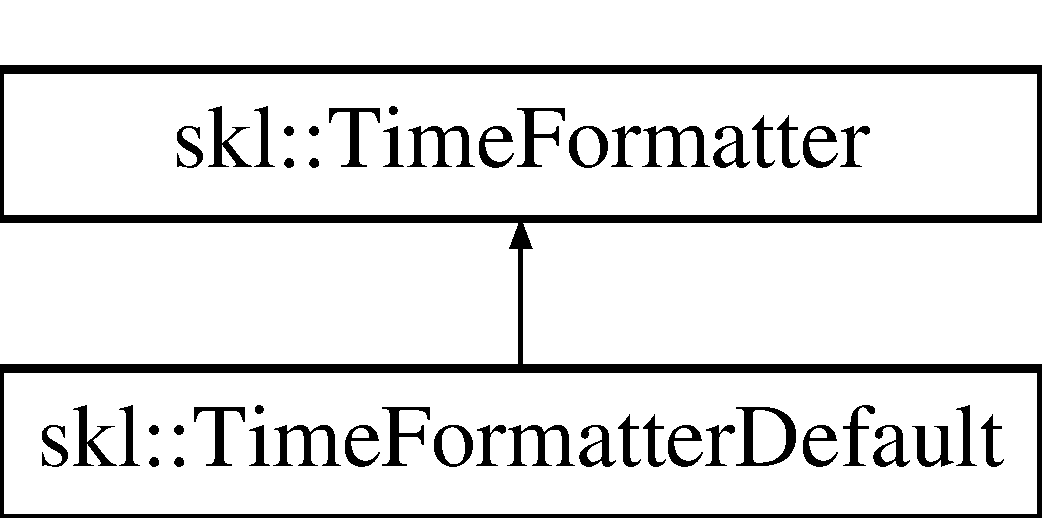
\includegraphics[height=2.000000cm]{classskl_1_1_time_formatter}
\end{center}
\end{figure}
\subsection*{Public Member Functions}
\begin{DoxyCompactItemize}
\item 
\hypertarget{classskl_1_1_time_formatter_a33a901eefd78aaadded7254a8005e3b8}{}\label{classskl_1_1_time_formatter_a33a901eefd78aaadded7254a8005e3b8} 
{\bfseries Time\+Formatter} (const std\+::string \&name=\char`\"{}\char`\"{})
\item 
\hypertarget{classskl_1_1_time_formatter_a10c8d84fe0fbe2abdec7962e319ffc40}{}\label{classskl_1_1_time_formatter_a10c8d84fe0fbe2abdec7962e319ffc40} 
virtual \hyperlink{classskl_1_1_time_formatter}{Time\+Formatter} $\ast$ {\bfseries clone} () const
\item 
\hypertarget{classskl_1_1_time_formatter_ac574740a7005255b669a8158729f1b80}{}\label{classskl_1_1_time_formatter_ac574740a7005255b669a8158729f1b80} 
virtual bool {\bfseries equals} (const \hyperlink{classskl_1_1_time_formatter}{Time\+Formatter} \&other) const
\item 
\hypertarget{classskl_1_1_time_formatter_aef33634872a38ff80019413edae56aeb}{}\label{classskl_1_1_time_formatter_aef33634872a38ff80019413edae56aeb} 
virtual void {\bfseries parse\+String} (const std\+::string \&str, int $\ast$Year, int $\ast$Mon, int $\ast$Day, int $\ast$Hour, int $\ast$Min, int $\ast$Sec, long $\ast$U\+Sec) const =0  throw (\+Time\+Format\+Exception)
\item 
\hypertarget{classskl_1_1_time_formatter_aa0028896c2c544917801268e97eb0a57}{}\label{classskl_1_1_time_formatter_aa0028896c2c544917801268e97eb0a57} 
virtual std\+::string {\bfseries to\+String} (int Year, int Mon, int Day, int Hour, int Min, int Sec, long U\+Sec) const =0
\item 
\hypertarget{classskl_1_1_time_formatter_af4f4ed9eef376bd3d920b56822873c0c}{}\label{classskl_1_1_time_formatter_af4f4ed9eef376bd3d920b56822873c0c} 
std\+::string {\bfseries get\+Name} () const
\end{DoxyCompactItemize}
\subsection*{Protected Member Functions}
\begin{DoxyCompactItemize}
\item 
\hypertarget{classskl_1_1_time_formatter_abe8fae39578eb6b94b4a669d679a7bf1}{}\label{classskl_1_1_time_formatter_abe8fae39578eb6b94b4a669d679a7bf1} 
{\bfseries Time\+Formatter} (const \hyperlink{classskl_1_1_time_formatter}{Time\+Formatter} \&other)
\end{DoxyCompactItemize}
\subsection*{Protected Attributes}
\begin{DoxyCompactItemize}
\item 
\hypertarget{classskl_1_1_time_formatter_a1a26b7ebf9f1a3e47942afecda7d3571}{}\label{classskl_1_1_time_formatter_a1a26b7ebf9f1a3e47942afecda7d3571} 
std\+::string {\bfseries name}
\end{DoxyCompactItemize}


\subsection{Detailed Description}
\hyperlink{classskl_1_1_time_formatter}{Time\+Formatter}\textquotesingle{}s abstrcut class. 

\hyperlink{classskl_1_1_time_formatter}{Time\+Formatter} 時間と文字列の相互変換を行う基底クラス(仮想) 

The documentation for this class was generated from the following files\+:\begin{DoxyCompactItemize}
\item 
Core/include/\hyperlink{_time_formatter_8h}{Time\+Formatter.\+h}\item 
Core/src/\hyperlink{_time_formatter_8cpp}{Time\+Formatter.\+cpp}\end{DoxyCompactItemize}

\hypertarget{classskl_1_1_time_formatter_default}{}\section{skl\+:\+:Time\+Formatter\+Default Class Reference}
\label{classskl_1_1_time_formatter_default}\index{skl\+::\+Time\+Formatter\+Default@{skl\+::\+Time\+Formatter\+Default}}


\hyperlink{classskl_1_1_time_formatter_default}{Time\+Formatter\+Default}.  




{\ttfamily \#include $<$Time\+Formatter\+Default.\+h$>$}

Inheritance diagram for skl\+:\+:Time\+Formatter\+Default\+:\begin{figure}[H]
\begin{center}
\leavevmode
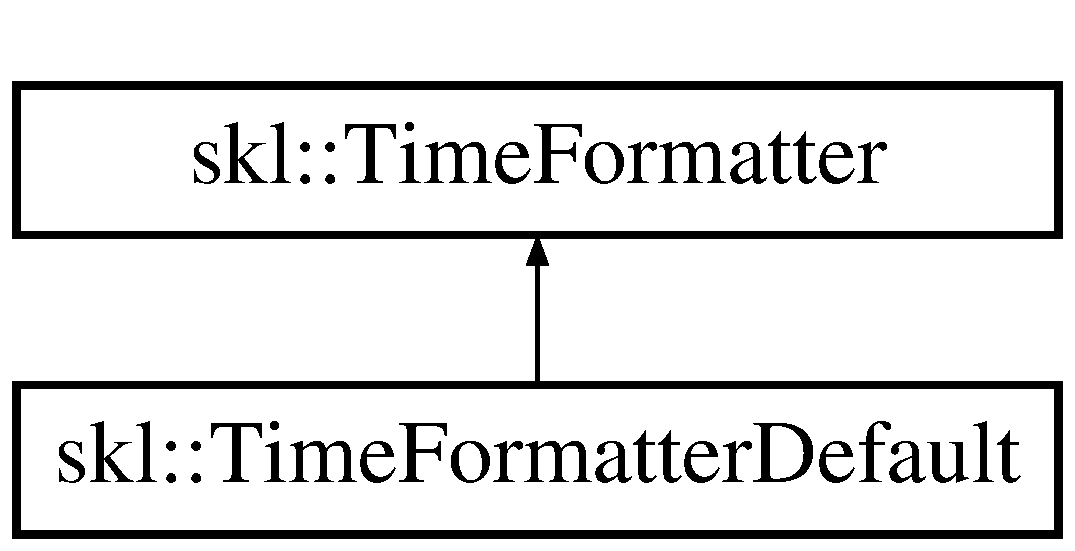
\includegraphics[height=2.000000cm]{classskl_1_1_time_formatter_default}
\end{center}
\end{figure}
\subsection*{Public Member Functions}
\begin{DoxyCompactItemize}
\item 
\hypertarget{classskl_1_1_time_formatter_default_a5cddc15b60b466a86a5f963de1ad8e90}{}\label{classskl_1_1_time_formatter_default_a5cddc15b60b466a86a5f963de1ad8e90} 
virtual \hyperlink{classskl_1_1_time_formatter_default}{Time\+Formatter\+Default} $\ast$ {\bfseries clone} () const
\item 
\hypertarget{classskl_1_1_time_formatter_default_a80774f6fcf15b18e7edb78a5e4d3c01a}{}\label{classskl_1_1_time_formatter_default_a80774f6fcf15b18e7edb78a5e4d3c01a} 
virtual bool {\bfseries equals} (const \hyperlink{classskl_1_1_time_formatter}{Time\+Formatter} \&other) const
\item 
void \hyperlink{classskl_1_1_time_formatter_default_a803104c1e78b366dc9f4c6fecb632c11}{parse\+String} (const std\+::string \&str, int $\ast$Year, int $\ast$Mon, int $\ast$Day, int $\ast$Hour, int $\ast$Min, int $\ast$Sec, long $\ast$U\+Sec) const  throw (\+Time\+Format\+Exception)
\begin{DoxyCompactList}\small\item\em 文字列を解析し,数字を代入する \end{DoxyCompactList}\item 
std\+::string \hyperlink{classskl_1_1_time_formatter_default_aa0636a112004da1d9646c127d10bf9d8}{to\+String} (int Year, int Mon, int Day, int Hour, int Min, int Sec, long U\+Sec) const
\begin{DoxyCompactList}\small\item\em 文字列へ変換する関数 \end{DoxyCompactList}\end{DoxyCompactItemize}
\subsection*{Protected Member Functions}
\begin{DoxyCompactItemize}
\item 
\hypertarget{classskl_1_1_time_formatter_default_ac96f3974a6623e1385d7dba188939ff9}{}\label{classskl_1_1_time_formatter_default_ac96f3974a6623e1385d7dba188939ff9} 
{\bfseries Time\+Formatter\+Default} (const \hyperlink{classskl_1_1_time_formatter_default}{Time\+Formatter\+Default} \&other)
\end{DoxyCompactItemize}
\subsection*{Additional Inherited Members}


\subsection{Detailed Description}
\hyperlink{classskl_1_1_time_formatter_default}{Time\+Formatter\+Default}. 

Y\+Y\+Y\+Y.\+M\+M.\+D\+D\+\_\+hh.\+mm.\+ss.\+fff 形式を扱う 

\subsection{Member Function Documentation}
\hypertarget{classskl_1_1_time_formatter_default_a803104c1e78b366dc9f4c6fecb632c11}{}\label{classskl_1_1_time_formatter_default_a803104c1e78b366dc9f4c6fecb632c11} 
\index{skl\+::\+Time\+Formatter\+Default@{skl\+::\+Time\+Formatter\+Default}!parse\+String@{parse\+String}}
\index{parse\+String@{parse\+String}!skl\+::\+Time\+Formatter\+Default@{skl\+::\+Time\+Formatter\+Default}}
\subsubsection{\texorpdfstring{parse\+String()}{parseString()}}
{\footnotesize\ttfamily void skl\+::\+Time\+Formatter\+Default\+::parse\+String (\begin{DoxyParamCaption}\item[{const std\+::string \&}]{str,  }\item[{int $\ast$}]{Year,  }\item[{int $\ast$}]{Mon,  }\item[{int $\ast$}]{Day,  }\item[{int $\ast$}]{Hour,  }\item[{int $\ast$}]{Min,  }\item[{int $\ast$}]{Sec,  }\item[{long $\ast$}]{U\+Sec }\end{DoxyParamCaption}) const throw  \hyperlink{classskl_1_1_time_format_exception}{Time\+Format\+Exception}) \hspace{0.3cm}{\ttfamily [virtual]}}



文字列を解析し,数字を代入する 


\begin{DoxyParams}{Parameters}
{\em str} & 解析する文字列 \\
\hline
{\em Year} & 年を入れる変数 \\
\hline
{\em Mon} & 月を入れる変数 \\
\hline
{\em Day} & 日を入れる変数 \\
\hline
{\em Hour} & 時を入れる変数 \\
\hline
{\em Min} & 分を入れる変数 \\
\hline
{\em Sec} & 秒を入れる変数 \\
\hline
{\em U\+Sec} & U\+Sec(micro sec.)を入れる変数 \\
\hline
\end{DoxyParams}


Implements \hyperlink{classskl_1_1_time_formatter}{skl\+::\+Time\+Formatter}.

\hypertarget{classskl_1_1_time_formatter_default_aa0636a112004da1d9646c127d10bf9d8}{}\label{classskl_1_1_time_formatter_default_aa0636a112004da1d9646c127d10bf9d8} 
\index{skl\+::\+Time\+Formatter\+Default@{skl\+::\+Time\+Formatter\+Default}!to\+String@{to\+String}}
\index{to\+String@{to\+String}!skl\+::\+Time\+Formatter\+Default@{skl\+::\+Time\+Formatter\+Default}}
\subsubsection{\texorpdfstring{to\+String()}{toString()}}
{\footnotesize\ttfamily std\+::string skl\+::\+Time\+Formatter\+Default\+::to\+String (\begin{DoxyParamCaption}\item[{int}]{Year,  }\item[{int}]{Mon,  }\item[{int}]{Day,  }\item[{int}]{Hour,  }\item[{int}]{Min,  }\item[{int}]{Sec,  }\item[{long}]{U\+Sec }\end{DoxyParamCaption}) const\hspace{0.3cm}{\ttfamily [virtual]}}



文字列へ変換する関数 


\begin{DoxyParams}{Parameters}
{\em Year} & 年 \\
\hline
{\em Mon} & 月 \\
\hline
{\em Day} & 日 \\
\hline
{\em Hour} & 時 \\
\hline
{\em Min} & 分 \\
\hline
{\em Sec} & 秒 \\
\hline
{\em U\+Sec} & マイクロ秒\\
\hline
\end{DoxyParams}
\begin{DoxyReturn}{Returns}
文字列表現 
\end{DoxyReturn}


Implements \hyperlink{classskl_1_1_time_formatter}{skl\+::\+Time\+Formatter}.



The documentation for this class was generated from the following files\+:\begin{DoxyCompactItemize}
\item 
Core/include/\hyperlink{_time_formatter_default_8h}{Time\+Formatter\+Default.\+h}\item 
Core/src/Time\+Formatter\+Default.\+cpp\end{DoxyCompactItemize}

\hypertarget{classskl_1_1_time_interval}{}\section{skl\+:\+:Time\+Interval Class Reference}
\label{classskl_1_1_time_interval}\index{skl\+::\+Time\+Interval@{skl\+::\+Time\+Interval}}


時間間隔を表すクラス(最小単位\+:msec)  




{\ttfamily \#include $<$Time\+Interval.\+h$>$}

Inheritance diagram for skl\+:\+:Time\+Interval\+:\begin{figure}[H]
\begin{center}
\leavevmode
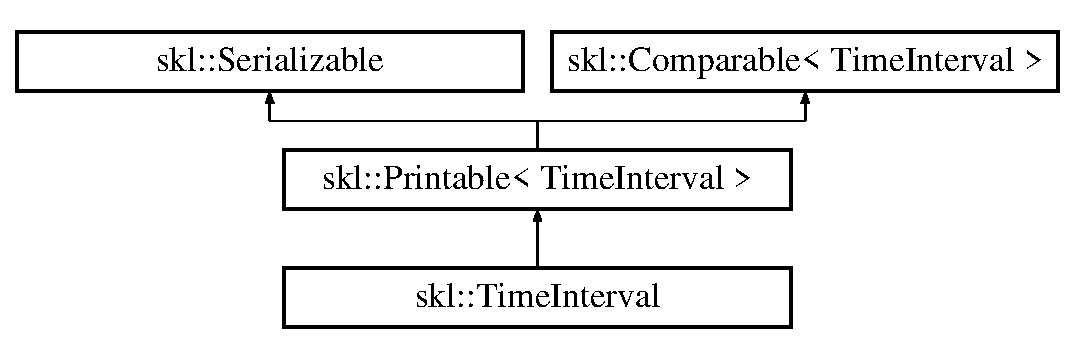
\includegraphics[height=3.000000cm]{classskl_1_1_time_interval}
\end{center}
\end{figure}
\subsection*{Public Member Functions}
\begin{DoxyCompactItemize}
\item 
\hypertarget{classskl_1_1_time_interval_adfa93f83372d9d25e27282ed38e35345}{}\label{classskl_1_1_time_interval_adfa93f83372d9d25e27282ed38e35345} 
\hyperlink{classskl_1_1_time_interval_adfa93f83372d9d25e27282ed38e35345}{Time\+Interval} (long long msec=0)
\begin{DoxyCompactList}\small\item\em デフォルトコンストラクタ \end{DoxyCompactList}\item 
\hypertarget{classskl_1_1_time_interval_a1d2f4f99ab2358c6c2c9d812835e50ce}{}\label{classskl_1_1_time_interval_a1d2f4f99ab2358c6c2c9d812835e50ce} 
\hyperlink{classskl_1_1_time_interval_a1d2f4f99ab2358c6c2c9d812835e50ce}{Time\+Interval} (long hour, int minute, int sec=0, int msec=0, int sign=1)
\begin{DoxyCompactList}\small\item\em 要素毎に指定するコンストラクタ \end{DoxyCompactList}\item 
\hypertarget{classskl_1_1_time_interval_aa0aa3a4fa4887826b0d194036891bb10}{}\label{classskl_1_1_time_interval_aa0aa3a4fa4887826b0d194036891bb10} 
\hyperlink{classskl_1_1_time_interval_aa0aa3a4fa4887826b0d194036891bb10}{Time\+Interval} (const std\+::string \&str)
\begin{DoxyCompactList}\small\item\em 文字列を引数にとるコンストラクタ \end{DoxyCompactList}\item 
\hypertarget{classskl_1_1_time_interval_a62581176e8c9c785d8a4c0a23ace8605}{}\label{classskl_1_1_time_interval_a62581176e8c9c785d8a4c0a23ace8605} 
\hyperlink{classskl_1_1_time_interval_a62581176e8c9c785d8a4c0a23ace8605}{Time\+Interval} (const \hyperlink{classskl_1_1_time_interval}{Time\+Interval} \&other)
\begin{DoxyCompactList}\small\item\em コピーコンストラクタ \end{DoxyCompactList}\item 
\hypertarget{classskl_1_1_time_interval_ab9e4f540a894261106ac579d1d409b23}{}\label{classskl_1_1_time_interval_ab9e4f540a894261106ac579d1d409b23} 
virtual \hyperlink{classskl_1_1_time_interval_ab9e4f540a894261106ac579d1d409b23}{$\sim$\+Time\+Interval} ()
\begin{DoxyCompactList}\small\item\em デストラクタ \end{DoxyCompactList}\item 
std\+::string \hyperlink{classskl_1_1_time_interval_a371c857881c27d68bff36e169646126a}{to\+String} () const
\begin{DoxyCompactList}\small\item\em 文字列として書き出す(本体はprint()) \end{DoxyCompactList}\item 
void \hyperlink{classskl_1_1_time_interval_ae706d4ce4795c566ce481f96380a878f}{parse\+String} (const std\+::string \&str)
\begin{DoxyCompactList}\small\item\em 文字列から読み出す(本体はscanで定義) \end{DoxyCompactList}\item 
std\+::string \hyperlink{classskl_1_1_time_interval_a1605c779683229ccc9e714f651ab3b1d}{print} () const
\begin{DoxyCompactList}\small\item\em 文字列として書き出す \end{DoxyCompactList}\item 
bool \hyperlink{classskl_1_1_time_interval_ac2ad9a1a830ce70e6702969815ca7468}{scan} (const std\+::string \&str)
\begin{DoxyCompactList}\small\item\em 文字列から読み出す \end{DoxyCompactList}\item 
double \hyperlink{classskl_1_1_time_interval_afa1dd3e11159f1f8886e83db1c11eb5a}{get\+As\+Second} () const
\begin{DoxyCompactList}\small\item\em millisecond以下を小数として、秒単位で取り出す \end{DoxyCompactList}\item 
\hypertarget{classskl_1_1_time_interval_a7b1ae87caad5ec9346f4c93415e3574f}{}\label{classskl_1_1_time_interval_a7b1ae87caad5ec9346f4c93415e3574f} 
{\bfseries operator long long} () const
\item 
\hypertarget{classskl_1_1_time_interval_a50850c985e918e73c2e189cd7666fa1d}{}\label{classskl_1_1_time_interval_a50850c985e918e73c2e189cd7666fa1d} 
bool \hyperlink{classskl_1_1_time_interval_a50850c985e918e73c2e189cd7666fa1d}{operator$<$} (const \hyperlink{classskl_1_1_time_interval}{Time\+Interval} \&other) const
\begin{DoxyCompactList}\small\item\em 比較演算子(但し、printした文字列の順序を利用するので、意味のある比較をした場合には具象クラス毎に定義すること) \end{DoxyCompactList}\item 
\hypertarget{classskl_1_1_time_interval_af2846332871234fdb1e6eb1b50ea3105}{}\label{classskl_1_1_time_interval_af2846332871234fdb1e6eb1b50ea3105} 
\hyperlink{classskl_1_1_time_interval}{Time\+Interval} \& {\bfseries operator=} (const \hyperlink{classskl_1_1_time_interval}{Time\+Interval} \&other)
\item 
\hypertarget{classskl_1_1_time_interval_a7b4730d6e3512cf5a81d984452b9ee3f}{}\label{classskl_1_1_time_interval_a7b4730d6e3512cf5a81d984452b9ee3f} 
long long {\bfseries operator-\/} (const \hyperlink{classskl_1_1_time_interval}{Time\+Interval} \&other) const
\item 
\hypertarget{classskl_1_1_time_interval_afe7e4bed83dfd04b54bac4fe7f68ebe5}{}\label{classskl_1_1_time_interval_afe7e4bed83dfd04b54bac4fe7f68ebe5} 
long long {\bfseries operator+} (const \hyperlink{classskl_1_1_time_interval}{Time\+Interval} \&other) const
\item 
\hypertarget{classskl_1_1_time_interval_a74ec9555c6d258bd3b8627a60ca5c634}{}\label{classskl_1_1_time_interval_a74ec9555c6d258bd3b8627a60ca5c634} 
\hyperlink{classskl_1_1_time_interval}{Time\+Interval} \& {\bfseries operator-\/=} (const \hyperlink{classskl_1_1_time_interval}{Time\+Interval} \&other)
\item 
\hypertarget{classskl_1_1_time_interval_a8a27f01d1abea70e9fea32aa79de79c3}{}\label{classskl_1_1_time_interval_a8a27f01d1abea70e9fea32aa79de79c3} 
\hyperlink{classskl_1_1_time_interval}{Time\+Interval} \& {\bfseries operator+=} (const \hyperlink{classskl_1_1_time_interval}{Time\+Interval} \&other)
\item 
\hypertarget{classskl_1_1_time_interval_a7a30ed02d174a90446b5788a674e0647}{}\label{classskl_1_1_time_interval_a7a30ed02d174a90446b5788a674e0647} 
long long {\bfseries operator-\/} () const
\item 
\hypertarget{classskl_1_1_time_interval_a3361133892254c113d238ab4ae0060f3}{}\label{classskl_1_1_time_interval_a3361133892254c113d238ab4ae0060f3} 
\hyperlink{classskl_1_1_time_interval}{Time\+Interval} \& {\bfseries operator\%=} (const \hyperlink{classskl_1_1_time_interval}{Time\+Interval} \&other)
\item 
\hypertarget{classskl_1_1_time_interval_aae7818a395cdf61c2672a80ddb73ae86}{}\label{classskl_1_1_time_interval_aae7818a395cdf61c2672a80ddb73ae86} 
\hyperlink{classskl_1_1_time_interval}{Time\+Interval} \& {\bfseries operator/=} (long long factor)
\item 
\hypertarget{classskl_1_1_time_interval_aa627ad5802fd80fb78af4c98d6b6a867}{}\label{classskl_1_1_time_interval_aa627ad5802fd80fb78af4c98d6b6a867} 
\hyperlink{classskl_1_1_time_interval}{Time\+Interval} \& {\bfseries operator$\ast$=} (long long factor)
\item 
\hypertarget{classskl_1_1_time_interval_ace5e1abd3590b0663a2d40ac6f4a0ff7}{}\label{classskl_1_1_time_interval_ace5e1abd3590b0663a2d40ac6f4a0ff7} 
long \hyperlink{classskl_1_1_time_interval_ace5e1abd3590b0663a2d40ac6f4a0ff7}{\+\_\+buf\+\_\+size} () const
\begin{DoxyCompactList}\small\item\em \+\_\+serializeで生成される予定のbufの長さを返す \end{DoxyCompactList}\item 
\hypertarget{classskl_1_1_time_interval_ae2a439599345ef0c813c2a37278bc50d}{}\label{classskl_1_1_time_interval_ae2a439599345ef0c813c2a37278bc50d} 
void \hyperlink{classskl_1_1_time_interval_ae2a439599345ef0c813c2a37278bc50d}{\+\_\+serialize} ()
\begin{DoxyCompactList}\small\item\em クラスの中身を直列化してメンバ変数のbufに格納する \end{DoxyCompactList}\item 
\hypertarget{classskl_1_1_time_interval_aabf6e35b9f1fe546f8b884cd7dc732fc}{}\label{classskl_1_1_time_interval_aabf6e35b9f1fe546f8b884cd7dc732fc} 
void \hyperlink{classskl_1_1_time_interval_aabf6e35b9f1fe546f8b884cd7dc732fc}{\+\_\+deserialize} (const char $\ast$\hyperlink{classskl_1_1_serializable_a1d203d9f0049ce37183a0dcefbc6399a}{buf}, long \hyperlink{classskl_1_1_serializable_a087eb19fada917a42b8411bfecbac0f1}{buf\+\_\+size})
\begin{DoxyCompactList}\small\item\em 直列化されたクラスの中身を読み込む \end{DoxyCompactList}\end{DoxyCompactItemize}
\subsection*{Protected Attributes}
\begin{DoxyCompactItemize}
\item 
\hypertarget{classskl_1_1_time_interval_a7992e2eaeba03bc07d341734d47f99d0}{}\label{classskl_1_1_time_interval_a7992e2eaeba03bc07d341734d47f99d0} 
long long {\bfseries msec}
\end{DoxyCompactItemize}
\subsection*{Additional Inherited Members}


\subsection{Detailed Description}
時間間隔を表すクラス(最小単位\+:msec) 

\subsection{Member Function Documentation}
\hypertarget{classskl_1_1_time_interval_afa1dd3e11159f1f8886e83db1c11eb5a}{}\label{classskl_1_1_time_interval_afa1dd3e11159f1f8886e83db1c11eb5a} 
\index{skl\+::\+Time\+Interval@{skl\+::\+Time\+Interval}!get\+As\+Second@{get\+As\+Second}}
\index{get\+As\+Second@{get\+As\+Second}!skl\+::\+Time\+Interval@{skl\+::\+Time\+Interval}}
\subsubsection{\texorpdfstring{get\+As\+Second()}{getAsSecond()}}
{\footnotesize\ttfamily double skl\+::\+Time\+Interval\+::get\+As\+Second (\begin{DoxyParamCaption}{ }\end{DoxyParamCaption}) const}



millisecond以下を小数として、秒単位で取り出す 

\begin{DoxyReturn}{Returns}
sec(double) 
\end{DoxyReturn}
\hypertarget{classskl_1_1_time_interval_ae706d4ce4795c566ce481f96380a878f}{}\label{classskl_1_1_time_interval_ae706d4ce4795c566ce481f96380a878f} 
\index{skl\+::\+Time\+Interval@{skl\+::\+Time\+Interval}!parse\+String@{parse\+String}}
\index{parse\+String@{parse\+String}!skl\+::\+Time\+Interval@{skl\+::\+Time\+Interval}}
\subsubsection{\texorpdfstring{parse\+String()}{parseString()}}
{\footnotesize\ttfamily void skl\+::\+Time\+Interval\+::parse\+String (\begin{DoxyParamCaption}\item[{const std\+::string \&}]{str }\end{DoxyParamCaption})}



文字列から読み出す(本体はscanで定義) 


\begin{DoxyParams}{Parameters}
{\em str} & (\mbox{[}-\/\mbox{]}H\+H\+:\+MM\+:S\+S.\+mmm)という書式でかかれた文字列 \\
\hline
\end{DoxyParams}
\hypertarget{classskl_1_1_time_interval_a1605c779683229ccc9e714f651ab3b1d}{}\label{classskl_1_1_time_interval_a1605c779683229ccc9e714f651ab3b1d} 
\index{skl\+::\+Time\+Interval@{skl\+::\+Time\+Interval}!print@{print}}
\index{print@{print}!skl\+::\+Time\+Interval@{skl\+::\+Time\+Interval}}
\subsubsection{\texorpdfstring{print()}{print()}}
{\footnotesize\ttfamily std\+::string skl\+::\+Time\+Interval\+::print (\begin{DoxyParamCaption}{ }\end{DoxyParamCaption}) const\hspace{0.3cm}{\ttfamily [virtual]}}



文字列として書き出す 


\begin{DoxyRetVals}{Return values}
{\em 時間情報の文字列(\mbox{[}-\/\mbox{]}\+H\+H\+:\+M\+M\+:\+S\+S.\+mmm)} & \\
\hline
\end{DoxyRetVals}


Implements \hyperlink{classskl_1_1_printable}{skl\+::\+Printable$<$ Time\+Interval $>$}.

\hypertarget{classskl_1_1_time_interval_ac2ad9a1a830ce70e6702969815ca7468}{}\label{classskl_1_1_time_interval_ac2ad9a1a830ce70e6702969815ca7468} 
\index{skl\+::\+Time\+Interval@{skl\+::\+Time\+Interval}!scan@{scan}}
\index{scan@{scan}!skl\+::\+Time\+Interval@{skl\+::\+Time\+Interval}}
\subsubsection{\texorpdfstring{scan()}{scan()}}
{\footnotesize\ttfamily bool skl\+::\+Time\+Interval\+::scan (\begin{DoxyParamCaption}\item[{const std\+::string \&}]{\+\_\+str }\end{DoxyParamCaption})\hspace{0.3cm}{\ttfamily [virtual]}}



文字列から読み出す 


\begin{DoxyParams}{Parameters}
{\em str} & (\mbox{[}-\/\mbox{]}H\+H\+:\+MM\+:S\+S.\+mmm)という書式でかかれた文字列 \\
\hline
\end{DoxyParams}


Implements \hyperlink{classskl_1_1_printable}{skl\+::\+Printable$<$ Time\+Interval $>$}.

\hypertarget{classskl_1_1_time_interval_a371c857881c27d68bff36e169646126a}{}\label{classskl_1_1_time_interval_a371c857881c27d68bff36e169646126a} 
\index{skl\+::\+Time\+Interval@{skl\+::\+Time\+Interval}!to\+String@{to\+String}}
\index{to\+String@{to\+String}!skl\+::\+Time\+Interval@{skl\+::\+Time\+Interval}}
\subsubsection{\texorpdfstring{to\+String()}{toString()}}
{\footnotesize\ttfamily std\+::string skl\+::\+Time\+Interval\+::to\+String (\begin{DoxyParamCaption}{ }\end{DoxyParamCaption}) const}



文字列として書き出す(本体はprint()) 


\begin{DoxyRetVals}{Return values}
{\em 時間情報の文字列(\mbox{[}-\/\mbox{]}\+H\+H\+:\+M\+M\+:\+S\+S.\+mmm)} & \\
\hline
\end{DoxyRetVals}


The documentation for this class was generated from the following files\+:\begin{DoxyCompactItemize}
\item 
Core/include/\hyperlink{_time_interval_8h}{Time\+Interval.\+h}\item 
Core/src/\hyperlink{_time_interval_8cpp}{Time\+Interval.\+cpp}\end{DoxyCompactItemize}

\hypertarget{classskl_1_1_touched_region_detector}{}\section{skl\+:\+:Touched\+Region\+Detector Class Reference}
\label{classskl_1_1_touched_region_detector}\index{skl\+::\+Touched\+Region\+Detector@{skl\+::\+Touched\+Region\+Detector}}


与えられたマスクから最近触られた物体のみを得る(入力はshort型のlabel画像  




{\ttfamily \#include $<$Touched\+Region\+Detector.\+h$>$}

Inheritance diagram for skl\+:\+:Touched\+Region\+Detector\+:\begin{figure}[H]
\begin{center}
\leavevmode
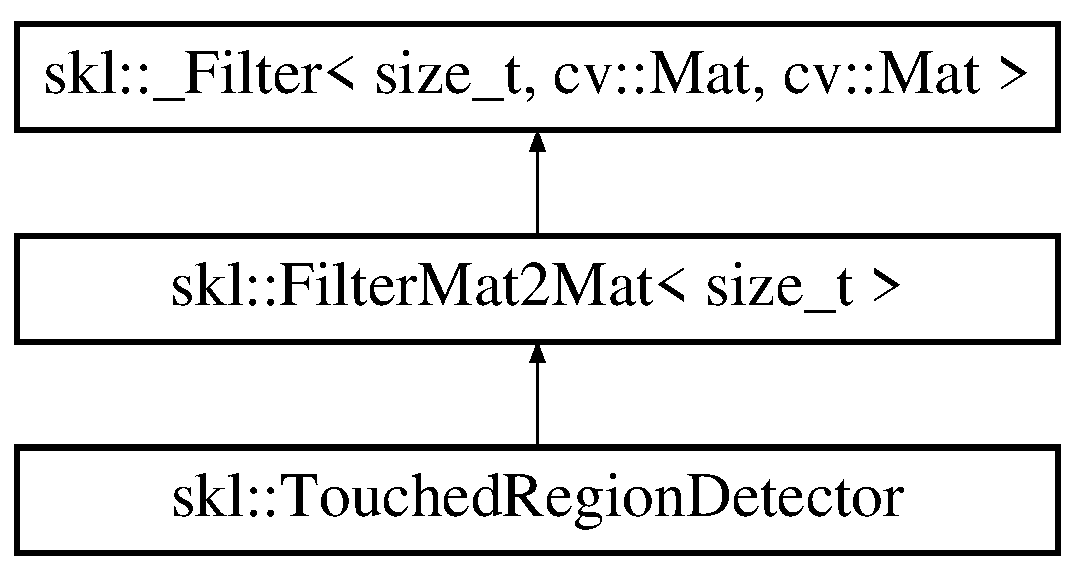
\includegraphics[height=3.000000cm]{classskl_1_1_touched_region_detector}
\end{center}
\end{figure}
\subsection*{Public Member Functions}
\begin{DoxyCompactItemize}
\item 
\hypertarget{classskl_1_1_touched_region_detector_a9665342f49cd4df671c960fd436bcab2}{}\label{classskl_1_1_touched_region_detector_a9665342f49cd4df671c960fd436bcab2} 
\hyperlink{classskl_1_1_touched_region_detector_a9665342f49cd4df671c960fd436bcab2}{Touched\+Region\+Detector} (int length\+\_\+of\+\_\+memory=8)
\begin{DoxyCompactList}\small\item\em デフォルトコンストラクタ \end{DoxyCompactList}\item 
\hypertarget{classskl_1_1_touched_region_detector_a46db7f12eee5abec5dcbe6bcd837d762}{}\label{classskl_1_1_touched_region_detector_a46db7f12eee5abec5dcbe6bcd837d762} 
virtual \hyperlink{classskl_1_1_touched_region_detector_a46db7f12eee5abec5dcbe6bcd837d762}{$\sim$\+Touched\+Region\+Detector} ()
\begin{DoxyCompactList}\small\item\em デストラクタ \end{DoxyCompactList}\item 
\hypertarget{classskl_1_1_touched_region_detector_a8350b9fb985faba891b60088fd2765d3}{}\label{classskl_1_1_touched_region_detector_a8350b9fb985faba891b60088fd2765d3} 
size\+\_\+t {\bfseries compute} (const cv\+::\+Mat \&object\+\_\+labels, const cv\+::\+Mat \&human\+\_\+mask, cv\+::\+Mat \&dest)
\item 
\hypertarget{classskl_1_1_touched_region_detector_a498025688c3dc4a6adceef0626213f67}{}\label{classskl_1_1_touched_region_detector_a498025688c3dc4a6adceef0626213f67} 
void {\bfseries clear} ()
\item 
\hypertarget{classskl_1_1_touched_region_detector_ace235a7ea7adccab07ebb76350e6e023}{}\label{classskl_1_1_touched_region_detector_ace235a7ea7adccab07ebb76350e6e023} 
void {\bfseries length\+\_\+of\+\_\+memory} (int \+\_\+length\+\_\+of\+\_\+memory)
\item 
\hypertarget{classskl_1_1_touched_region_detector_ad1de05484be3a50b07a50f1242c9dc17}{}\label{classskl_1_1_touched_region_detector_ad1de05484be3a50b07a50f1242c9dc17} 
int {\bfseries length\+\_\+of\+\_\+memory} () const
\item 
\hypertarget{classskl_1_1_touched_region_detector_a9421371c23730541235eabf18e233797}{}\label{classskl_1_1_touched_region_detector_a9421371c23730541235eabf18e233797} 
const cv\+::\+Mat {\bfseries motion\+\_\+history\+\_\+image} () const
\end{DoxyCompactItemize}
\subsection*{Protected Attributes}
\begin{DoxyCompactItemize}
\item 
\hypertarget{classskl_1_1_touched_region_detector_aa1289b698bb2473f091f124f2a603cfa}{}\label{classskl_1_1_touched_region_detector_aa1289b698bb2473f091f124f2a603cfa} 
\hyperlink{classskl_1_1_motion_history}{Motion\+History} {\bfseries motion\+\_\+history\+\_\+algo}
\end{DoxyCompactItemize}


\subsection{Detailed Description}
与えられたマスクから最近触られた物体のみを得る(入力はshort型のlabel画像 

The documentation for this class was generated from the following files\+:\begin{DoxyCompactItemize}
\item 
Open\+C\+V/include/\hyperlink{_touched_region_detector_8h}{Touched\+Region\+Detector.\+h}\item 
Open\+C\+V/src/\hyperlink{_touched_region_detector_8cpp}{Touched\+Region\+Detector.\+cpp}\end{DoxyCompactItemize}

\hypertarget{classskl_1_1_video_capture}{}\section{skl\+:\+:Video\+Capture Class Reference}
\label{classskl_1_1_video_capture}\index{skl\+::\+Video\+Capture@{skl\+::\+Video\+Capture}}


パラメタの読み込み機能などを強化した\+Video\+Capture  




{\ttfamily \#include $<$skl\+Video\+Capture.\+h$>$}

Inheritance diagram for skl\+:\+:Video\+Capture\+:\begin{figure}[H]
\begin{center}
\leavevmode
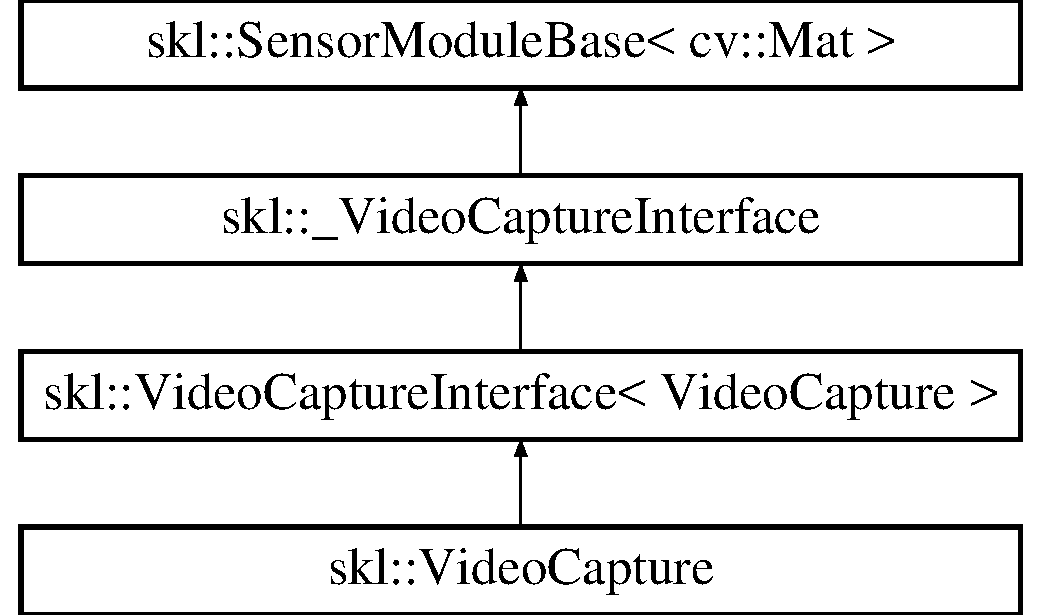
\includegraphics[height=4.000000cm]{classskl_1_1_video_capture}
\end{center}
\end{figure}
\subsection*{Public Member Functions}
\begin{DoxyCompactItemize}
\item 
\hypertarget{classskl_1_1_video_capture_a6a80b08bcec34f70cb88c5d0a2673203}{}\label{classskl_1_1_video_capture_a6a80b08bcec34f70cb88c5d0a2673203} 
\hyperlink{classskl_1_1_video_capture_a6a80b08bcec34f70cb88c5d0a2673203}{Video\+Capture} ()
\begin{DoxyCompactList}\small\item\em デフォルトコンストラクタ \end{DoxyCompactList}\item 
\hypertarget{classskl_1_1_video_capture_a7acc372d7e02d7c33de77c3fc0d2b3ef}{}\label{classskl_1_1_video_capture_a7acc372d7e02d7c33de77c3fc0d2b3ef} 
virtual \hyperlink{classskl_1_1_video_capture_a7acc372d7e02d7c33de77c3fc0d2b3ef}{$\sim$\+Video\+Capture} ()
\begin{DoxyCompactList}\small\item\em デストラクタ \end{DoxyCompactList}\item 
\hypertarget{classskl_1_1_video_capture_aed05a9295d8a04e208d79036f93aad64}{}\label{classskl_1_1_video_capture_aed05a9295d8a04e208d79036f93aad64} 
bool {\bfseries open} (const std\+::string \&filename)
\item 
\hypertarget{classskl_1_1_video_capture_af1f5af87dc823381e91e9bf117186896}{}\label{classskl_1_1_video_capture_af1f5af87dc823381e91e9bf117186896} 
bool {\bfseries open} (const std\+::string \&filename, cv\+::\+Ptr$<$ \hyperlink{classskl_1_1___video_capture_interface}{\+\_\+\+Video\+Capture\+Interface} $>$ cam)
\item 
\hypertarget{classskl_1_1_video_capture_a0cf51b1a893f88b68a5fe9b0a68c5002}{}\label{classskl_1_1_video_capture_a0cf51b1a893f88b68a5fe9b0a68c5002} 
bool {\bfseries open} (int device)
\item 
\hypertarget{classskl_1_1_video_capture_ab17630e9ffd76d49873ce5e60f4080f3}{}\label{classskl_1_1_video_capture_ab17630e9ffd76d49873ce5e60f4080f3} 
bool {\bfseries open} (int device, cv\+::\+Ptr$<$ \hyperlink{classskl_1_1___video_capture_interface}{\+\_\+\+Video\+Capture\+Interface} $>$ cam)
\item 
\hypertarget{classskl_1_1_video_capture_aa664b583d72ab38614a28644e7cd39fa}{}\label{classskl_1_1_video_capture_aa664b583d72ab38614a28644e7cd39fa} 
{\footnotesize template$<$class Iter $>$ }\\bool {\bfseries open} (Iter first, Iter last)
\item 
\hypertarget{classskl_1_1_video_capture_a773c26b4a2c6170493aabdb868759a0a}{}\label{classskl_1_1_video_capture_a773c26b4a2c6170493aabdb868759a0a} 
{\footnotesize template$<$class Iter , class cam\+Iter $>$ }\\bool {\bfseries open} (Iter first, Iter last)
\item 
\hypertarget{classskl_1_1_video_capture_a790296dad60b4f543c602980af45089f}{}\label{classskl_1_1_video_capture_a790296dad60b4f543c602980af45089f} 
bool {\bfseries is\+Opened} () const
\item 
\hypertarget{classskl_1_1_video_capture_ada3c7e5bb255553692092501df51e132}{}\label{classskl_1_1_video_capture_ada3c7e5bb255553692092501df51e132} 
void \hyperlink{classskl_1_1_video_capture_ada3c7e5bb255553692092501df51e132}{release} ()
\begin{DoxyCompactList}\small\item\em センサを特定する情報を入力する \end{DoxyCompactList}\item 
\hypertarget{classskl_1_1_video_capture_a7bb64b1a7e620908841b5fbaea3179e4}{}\label{classskl_1_1_video_capture_a7bb64b1a7e620908841b5fbaea3179e4} 
bool {\bfseries grab} ()
\item 
\hypertarget{classskl_1_1_video_capture_a6dedcb929497a8368c6865cda807e437}{}\label{classskl_1_1_video_capture_a6dedcb929497a8368c6865cda807e437} 
virtual bool {\bfseries retrieve} (cv\+::\+Mat \&image, int channel=0)
\item 
\hypertarget{classskl_1_1_video_capture_a705b31fcb25b91f8c4d4fdcc1e7c43a0}{}\label{classskl_1_1_video_capture_a705b31fcb25b91f8c4d4fdcc1e7c43a0} 
bool \hyperlink{classskl_1_1_video_capture_a705b31fcb25b91f8c4d4fdcc1e7c43a0}{set} (capture\+\_\+property\+\_\+t prop\+\_\+id, double val)
\begin{DoxyCompactList}\small\item\em カメラに値やモード(camera\+\_\+mode\+\_\+tがset($\ast$,camera\+\_\+mode\+\_\+t mode)を通してvalに与えられる(modeは-\/4から-\/1までの整数)をセットする純粋仮想関数 \end{DoxyCompactList}\item 
\hypertarget{classskl_1_1_video_capture_a3185737070044f7b729ae2c03dcb8fee}{}\label{classskl_1_1_video_capture_a3185737070044f7b729ae2c03dcb8fee} 
double \hyperlink{classskl_1_1_video_capture_a3185737070044f7b729ae2c03dcb8fee}{get} (capture\+\_\+property\+\_\+t prop\+\_\+id)
\begin{DoxyCompactList}\small\item\em カメラから値をgetする純粋仮想関数(modeはインターフェイス簡素化のためサポートしない) \end{DoxyCompactList}\item 
\hypertarget{classskl_1_1_video_capture_a1c650a65c8072ea844ab9e247e5eae96}{}\label{classskl_1_1_video_capture_a1c650a65c8072ea844ab9e247e5eae96} 
\hyperlink{classskl_1_1___video_capture_interface}{\+\_\+\+Video\+Capture\+Interface} \& {\bfseries operator\mbox{[}$\,$\mbox{]}} (int device)
\item 
\hypertarget{classskl_1_1_video_capture_a4ba435f10c75843873e92dc08b2ac918}{}\label{classskl_1_1_video_capture_a4ba435f10c75843873e92dc08b2ac918} 
size\+\_\+t {\bfseries size} () const
\item 
\hypertarget{classskl_1_1_video_capture_a928fdf909a9f7afaecc2bce578bb0702}{}\label{classskl_1_1_video_capture_a928fdf909a9f7afaecc2bce578bb0702} 
virtual bool {\bfseries push\+\_\+back} (const std\+::string \&filename)
\item 
\hypertarget{classskl_1_1_video_capture_abc326dce402d6bab7daacfcc953eaf7f}{}\label{classskl_1_1_video_capture_abc326dce402d6bab7daacfcc953eaf7f} 
virtual bool {\bfseries push\+\_\+back} (int device)
\item 
\hypertarget{classskl_1_1_video_capture_aa10a352ee8e1e795607f6df8917f3c35}{}\label{classskl_1_1_video_capture_aa10a352ee8e1e795607f6df8917f3c35} 
virtual bool {\bfseries push\+\_\+back} (const std\+::string \&filename, cv\+::\+Ptr$<$ \hyperlink{classskl_1_1___video_capture_interface}{\+\_\+\+Video\+Capture\+Interface} $>$ cam)
\item 
\hypertarget{classskl_1_1_video_capture_ac5d9f95727f61e5a619bcb5becb41f6c}{}\label{classskl_1_1_video_capture_ac5d9f95727f61e5a619bcb5becb41f6c} 
virtual bool {\bfseries push\+\_\+back} (int device, cv\+::\+Ptr$<$ \hyperlink{classskl_1_1___video_capture_interface}{\+\_\+\+Video\+Capture\+Interface} $>$ cam)
\item 
\hypertarget{classskl_1_1_video_capture_a59c8002f5400c9701b14b0f8230e9d05}{}\label{classskl_1_1_video_capture_a59c8002f5400c9701b14b0f8230e9d05} 
\hyperlink{classskl_1_1_video_capture}{Video\+Capture} \& {\bfseries operator$>$$>$} (std\+::vector$<$ cv\+::\+Mat $>$ \&mat\+\_\+vec)
\item 
\hypertarget{classskl_1_1_video_capture_acb223f8f69501dfe3127a1769e251db1}{}\label{classskl_1_1_video_capture_acb223f8f69501dfe3127a1769e251db1} 
cv\+::\+Ptr$<$ \hyperlink{classskl_1_1___video_capture_interface}{\+\_\+\+Video\+Capture\+Interface} $>$ \& {\bfseries operator\mbox{[}$\,$\mbox{]}} (size\+\_\+t i)
\item 
\hypertarget{classskl_1_1_video_capture_ae1ab532c19ac61856952c81de149d594}{}\label{classskl_1_1_video_capture_ae1ab532c19ac61856952c81de149d594} 
const cv\+::\+Ptr$<$ \hyperlink{classskl_1_1___video_capture_interface}{\+\_\+\+Video\+Capture\+Interface} $>$ \& {\bfseries operator\mbox{[}$\,$\mbox{]}} (size\+\_\+t i) const
\end{DoxyCompactItemize}
\subsection*{Protected Attributes}
\begin{DoxyCompactItemize}
\item 
\hypertarget{classskl_1_1_video_capture_a6b399c2cd88317a93d306e6db3b5c47e}{}\label{classskl_1_1_video_capture_a6b399c2cd88317a93d306e6db3b5c47e} 
std\+::vector$<$ cv\+::\+Ptr$<$ \hyperlink{classskl_1_1___video_capture_interface}{\+\_\+\+Video\+Capture\+Interface} $>$ $>$ {\bfseries cam\+\_\+interface}
\end{DoxyCompactItemize}


\subsection{Detailed Description}
パラメタの読み込み機能などを強化した\+Video\+Capture 

The documentation for this class was generated from the following files\+:\begin{DoxyCompactItemize}
\item 
Open\+C\+V/include/skl\+Video\+Capture.\+h\item 
Open\+C\+V/src/skl\+Video\+Capture.\+cpp\end{DoxyCompactItemize}

\hypertarget{class_video_capture__parallel__retrieve}{}\section{Video\+Capture\+\_\+parallel\+\_\+retrieve Class Reference}
\label{class_video_capture__parallel__retrieve}\index{Video\+Capture\+\_\+parallel\+\_\+retrieve@{Video\+Capture\+\_\+parallel\+\_\+retrieve}}
\subsection*{Public Member Functions}
\begin{DoxyCompactItemize}
\item 
\hypertarget{class_video_capture__parallel__retrieve_a9aa9a156ad89b16bd277916dfce58470}{}\label{class_video_capture__parallel__retrieve_a9aa9a156ad89b16bd277916dfce58470} 
{\bfseries Video\+Capture\+\_\+parallel\+\_\+retrieve} (std\+::vector$<$ cv\+::\+Ptr$<$ \hyperlink{classskl_1_1___video_capture_interface}{\+\_\+\+Video\+Capture\+Interface} $>$ $>$ \&cam\+\_\+interface, std\+::vector$<$ cv\+::\+Mat $>$ \&mat\+\_\+vec)
\item 
\hypertarget{class_video_capture__parallel__retrieve_a6c31905a8419293aaaf6ca7d33c94751}{}\label{class_video_capture__parallel__retrieve_a6c31905a8419293aaaf6ca7d33c94751} 
void {\bfseries operator()} (const cv\+::\+Blocked\+Range \&range) const
\end{DoxyCompactItemize}
\subsection*{Protected Attributes}
\begin{DoxyCompactItemize}
\item 
\hypertarget{class_video_capture__parallel__retrieve_a9afe7f600b55c958c9dcc5acc155df55}{}\label{class_video_capture__parallel__retrieve_a9afe7f600b55c958c9dcc5acc155df55} 
std\+::vector$<$ cv\+::\+Ptr$<$ \hyperlink{classskl_1_1___video_capture_interface}{\+\_\+\+Video\+Capture\+Interface} $>$ $>$ \& {\bfseries cam\+\_\+interface}
\item 
\hypertarget{class_video_capture__parallel__retrieve_a5c062539facc1c208ecfca311eba0323}{}\label{class_video_capture__parallel__retrieve_a5c062539facc1c208ecfca311eba0323} 
std\+::vector$<$ cv\+::\+Mat $>$ \& {\bfseries mat\+\_\+vec}
\end{DoxyCompactItemize}


The documentation for this class was generated from the following file\+:\begin{DoxyCompactItemize}
\item 
Open\+C\+V/src/skl\+Video\+Capture.\+cpp\end{DoxyCompactItemize}

\hypertarget{classskl_1_1_video_capture_default}{}\section{skl\+:\+:Video\+Capture\+Default Class Reference}
\label{classskl_1_1_video_capture_default}\index{skl\+::\+Video\+Capture\+Default@{skl\+::\+Video\+Capture\+Default}}


Open\+C\+Vのcv\+::\+Video\+Captureを利用する\+Video\+Capture.  




{\ttfamily \#include $<$Video\+Capture\+Default.\+h$>$}

Inheritance diagram for skl\+:\+:Video\+Capture\+Default\+:\begin{figure}[H]
\begin{center}
\leavevmode
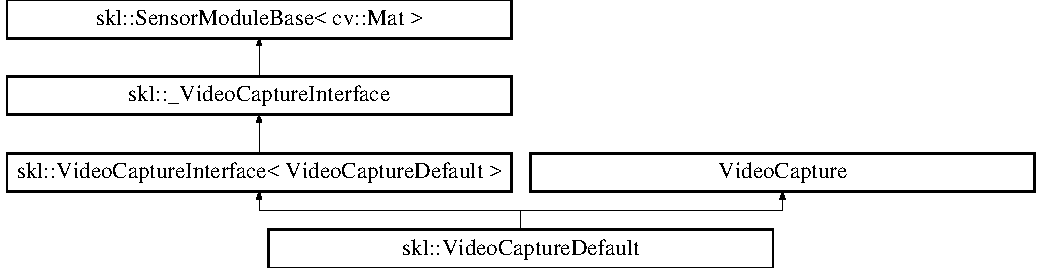
\includegraphics[height=3.601286cm]{classskl_1_1_video_capture_default}
\end{center}
\end{figure}
\subsection*{Public Member Functions}
\begin{DoxyCompactItemize}
\item 
\hypertarget{classskl_1_1_video_capture_default_a1c4eac1dbe596afa16d3663947260004}{}\label{classskl_1_1_video_capture_default_a1c4eac1dbe596afa16d3663947260004} 
\hyperlink{classskl_1_1_video_capture_default_a1c4eac1dbe596afa16d3663947260004}{Video\+Capture\+Default} ()
\begin{DoxyCompactList}\small\item\em デフォルトコンストラクタ \end{DoxyCompactList}\item 
\hypertarget{classskl_1_1_video_capture_default_ab80757b0119e28a212e4e9a7c966c883}{}\label{classskl_1_1_video_capture_default_ab80757b0119e28a212e4e9a7c966c883} 
virtual \hyperlink{classskl_1_1_video_capture_default_ab80757b0119e28a212e4e9a7c966c883}{$\sim$\+Video\+Capture\+Default} ()
\begin{DoxyCompactList}\small\item\em デストラクタ \end{DoxyCompactList}\item 
\hypertarget{classskl_1_1_video_capture_default_ac0898bf274ee0acf05fbbe895229c21b}{}\label{classskl_1_1_video_capture_default_ac0898bf274ee0acf05fbbe895229c21b} 
bool {\bfseries open} (const std\+::string \&filename)
\item 
\hypertarget{classskl_1_1_video_capture_default_afb80319eef496baba0ab45fc1b040ff2}{}\label{classskl_1_1_video_capture_default_afb80319eef496baba0ab45fc1b040ff2} 
bool {\bfseries open} (int device)
\item 
\hypertarget{classskl_1_1_video_capture_default_a6c6045af240272db07a981b605174dff}{}\label{classskl_1_1_video_capture_default_a6c6045af240272db07a981b605174dff} 
bool {\bfseries is\+Opened} () const
\item 
\hypertarget{classskl_1_1_video_capture_default_a4d86ae1172274a23cc401f2ca4116a5c}{}\label{classskl_1_1_video_capture_default_a4d86ae1172274a23cc401f2ca4116a5c} 
void \hyperlink{classskl_1_1_video_capture_default_a4d86ae1172274a23cc401f2ca4116a5c}{release} ()
\begin{DoxyCompactList}\small\item\em センサを特定する情報を入力する \end{DoxyCompactList}\item 
\hypertarget{classskl_1_1_video_capture_default_a0667bbfc63c734b78fc5db51e7329419}{}\label{classskl_1_1_video_capture_default_a0667bbfc63c734b78fc5db51e7329419} 
bool {\bfseries grab} ()
\item 
\hypertarget{classskl_1_1_video_capture_default_ab606b047d7d5e94c6aee600c2674a3b3}{}\label{classskl_1_1_video_capture_default_ab606b047d7d5e94c6aee600c2674a3b3} 
bool {\bfseries retrieve} (cv\+::\+Mat \&image, int channel=0)
\item 
\hypertarget{classskl_1_1_video_capture_default_a626a3b49fd2ba92cc3f39a59513e8414}{}\label{classskl_1_1_video_capture_default_a626a3b49fd2ba92cc3f39a59513e8414} 
bool \hyperlink{classskl_1_1_video_capture_default_a626a3b49fd2ba92cc3f39a59513e8414}{set} (capture\+\_\+property\+\_\+t prop\+\_\+id, double val)
\begin{DoxyCompactList}\small\item\em カメラに値やモード(camera\+\_\+mode\+\_\+tがset($\ast$,camera\+\_\+mode\+\_\+t mode)を通してvalに与えられる(modeは-\/4から-\/1までの整数)をセットする純粋仮想関数 \end{DoxyCompactList}\item 
\hypertarget{classskl_1_1_video_capture_default_a17131b806cb6f62a159e3459f2c1a724}{}\label{classskl_1_1_video_capture_default_a17131b806cb6f62a159e3459f2c1a724} 
double \hyperlink{classskl_1_1_video_capture_default_a17131b806cb6f62a159e3459f2c1a724}{get} (capture\+\_\+property\+\_\+t prop\+\_\+id)
\begin{DoxyCompactList}\small\item\em カメラから値をgetする純粋仮想関数(modeはインターフェイス簡素化のためサポートしない) \end{DoxyCompactList}\end{DoxyCompactItemize}
\subsection*{Protected Attributes}
\begin{DoxyCompactItemize}
\item 
\hypertarget{classskl_1_1_video_capture_default_a6965fe5cd25ec2aa2eeac3c002b306e8}{}\label{classskl_1_1_video_capture_default_a6965fe5cd25ec2aa2eeac3c002b306e8} 
cv\+::\+Mat {\bfseries buf}
\end{DoxyCompactItemize}


\subsection{Detailed Description}
Open\+C\+Vのcv\+::\+Video\+Captureを利用する\+Video\+Capture. 

The documentation for this class was generated from the following files\+:\begin{DoxyCompactItemize}
\item 
Open\+C\+V/include/\hyperlink{_video_capture_default_8h}{Video\+Capture\+Default.\+h}\item 
Open\+C\+V/src/\hyperlink{_video_capture_default_8cpp}{Video\+Capture\+Default.\+cpp}\end{DoxyCompactItemize}

\hypertarget{classskl_1_1gpu_1_1_video_capture_gpu}{}\section{skl\+:\+:gpu\+:\+:Video\+Capture\+Gpu Class Reference}
\label{classskl_1_1gpu_1_1_video_capture_gpu}\index{skl\+::gpu\+::\+Video\+Capture\+Gpu@{skl\+::gpu\+::\+Video\+Capture\+Gpu}}


cv\+::gpu\+::\+Gpu\+Matを返すキャプチャ。処理中に次のフレームを非同期でdeviceに送る分、連続フレームに対する処理が高速化される。  




{\ttfamily \#include $<$Video\+Capture\+Gpu.\+h$>$}

Inheritance diagram for skl\+:\+:gpu\+:\+:Video\+Capture\+Gpu\+:\begin{figure}[H]
\begin{center}
\leavevmode
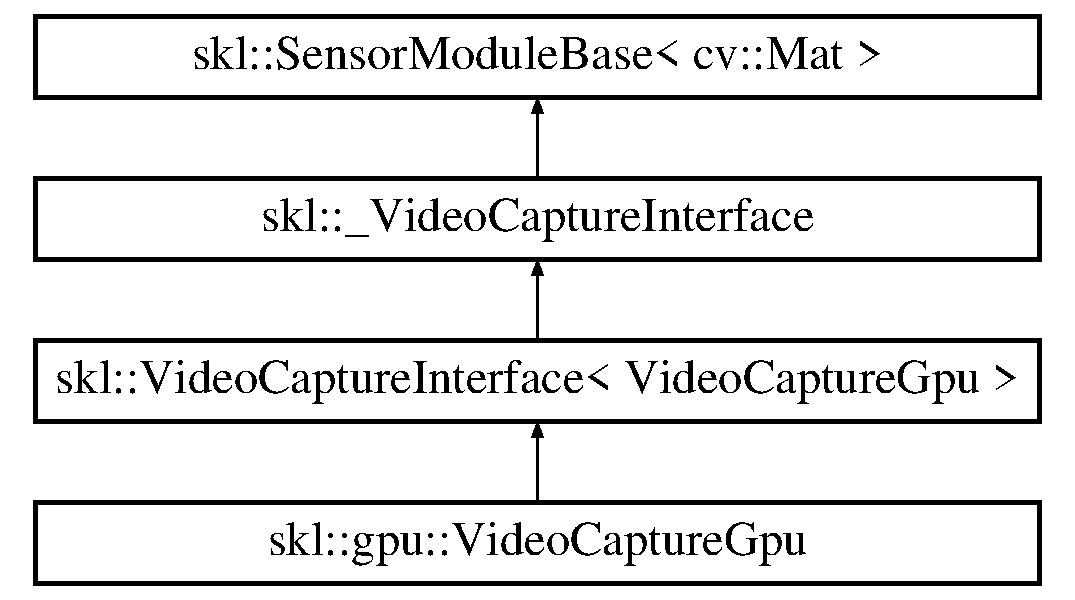
\includegraphics[height=4.000000cm]{classskl_1_1gpu_1_1_video_capture_gpu}
\end{center}
\end{figure}
\subsection*{Public Member Functions}
\begin{DoxyCompactItemize}
\item 
\hypertarget{classskl_1_1gpu_1_1_video_capture_gpu_ae1f7efcbf9ad654fbaec674d2c282c40}{}\label{classskl_1_1gpu_1_1_video_capture_gpu_ae1f7efcbf9ad654fbaec674d2c282c40} 
\hyperlink{classskl_1_1gpu_1_1_video_capture_gpu_ae1f7efcbf9ad654fbaec674d2c282c40}{Video\+Capture\+Gpu} (Video\+Capture\+Ptr video\+\_\+capture\+\_\+cpu=Video\+Capture\+Ptr())
\begin{DoxyCompactList}\small\item\em デフォルトコンストラクタ \end{DoxyCompactList}\item 
\hypertarget{classskl_1_1gpu_1_1_video_capture_gpu_a5e357372ee3f6717d8d407617178dc8c}{}\label{classskl_1_1gpu_1_1_video_capture_gpu_a5e357372ee3f6717d8d407617178dc8c} 
virtual \hyperlink{classskl_1_1gpu_1_1_video_capture_gpu_a5e357372ee3f6717d8d407617178dc8c}{$\sim$\+Video\+Capture\+Gpu} ()
\begin{DoxyCompactList}\small\item\em デストラクタ \end{DoxyCompactList}\item 
\hypertarget{classskl_1_1gpu_1_1_video_capture_gpu_a5db6d5866b7be0673457872cfe9c8714}{}\label{classskl_1_1gpu_1_1_video_capture_gpu_a5db6d5866b7be0673457872cfe9c8714} 
void {\bfseries set\+Base\+Capture} (Video\+Capture\+Ptr video\+\_\+capture\+\_\+cpu)
\item 
\hypertarget{classskl_1_1gpu_1_1_video_capture_gpu_a9de0b1d144534e21d5a0c169966a2765}{}\label{classskl_1_1gpu_1_1_video_capture_gpu_a9de0b1d144534e21d5a0c169966a2765} 
bool {\bfseries open} (const std\+::string \&filename)
\item 
\hypertarget{classskl_1_1gpu_1_1_video_capture_gpu_a1d45dcb80d7ac64f30ac02fb3ee44af6}{}\label{classskl_1_1gpu_1_1_video_capture_gpu_a1d45dcb80d7ac64f30ac02fb3ee44af6} 
bool {\bfseries open} (int device)
\item 
\hypertarget{classskl_1_1gpu_1_1_video_capture_gpu_a1253eef48a2b45e7ca355c82c7cf3ff0}{}\label{classskl_1_1gpu_1_1_video_capture_gpu_a1253eef48a2b45e7ca355c82c7cf3ff0} 
bool {\bfseries is\+Opened} () const
\item 
\hypertarget{classskl_1_1gpu_1_1_video_capture_gpu_ad9ccd9142fac1bfd4564df8ef660b8a8}{}\label{classskl_1_1gpu_1_1_video_capture_gpu_ad9ccd9142fac1bfd4564df8ef660b8a8} 
void \hyperlink{classskl_1_1gpu_1_1_video_capture_gpu_ad9ccd9142fac1bfd4564df8ef660b8a8}{release} ()
\begin{DoxyCompactList}\small\item\em センサを特定する情報を入力する \end{DoxyCompactList}\item 
\hypertarget{classskl_1_1gpu_1_1_video_capture_gpu_a3dd8b97a47ca09b6f1414f68ba434be3}{}\label{classskl_1_1gpu_1_1_video_capture_gpu_a3dd8b97a47ca09b6f1414f68ba434be3} 
bool {\bfseries grab} ()
\item 
\hypertarget{classskl_1_1gpu_1_1_video_capture_gpu_a83b956c7c450fa40045437f97acfef2e}{}\label{classskl_1_1gpu_1_1_video_capture_gpu_a83b956c7c450fa40045437f97acfef2e} 
virtual bool {\bfseries retrieve} (cv\+::\+Mat \&image, int channel=0)
\item 
\hypertarget{classskl_1_1gpu_1_1_video_capture_gpu_af969b32c8038ecdbf9c241f2e01fbb43}{}\label{classskl_1_1gpu_1_1_video_capture_gpu_af969b32c8038ecdbf9c241f2e01fbb43} 
virtual bool {\bfseries retrieve} (cv\+::gpu\+::\+Gpu\+Mat \&image, int channel=0)
\item 
\hypertarget{classskl_1_1gpu_1_1_video_capture_gpu_a10caf8a02f18b92b0ae3bd0c88c51469}{}\label{classskl_1_1gpu_1_1_video_capture_gpu_a10caf8a02f18b92b0ae3bd0c88c51469} 
bool \hyperlink{classskl_1_1gpu_1_1_video_capture_gpu_a10caf8a02f18b92b0ae3bd0c88c51469}{set} (capture\+\_\+property\+\_\+t prop\+\_\+id, double val)
\begin{DoxyCompactList}\small\item\em カメラに値やモード(camera\+\_\+mode\+\_\+tがset($\ast$,camera\+\_\+mode\+\_\+t mode)を通してvalに与えられる(modeは-\/4から-\/1までの整数)をセットする純粋仮想関数 \end{DoxyCompactList}\item 
\hypertarget{classskl_1_1gpu_1_1_video_capture_gpu_ad13971c83c79a3507d529a4602cb98de}{}\label{classskl_1_1gpu_1_1_video_capture_gpu_ad13971c83c79a3507d529a4602cb98de} 
double \hyperlink{classskl_1_1gpu_1_1_video_capture_gpu_ad13971c83c79a3507d529a4602cb98de}{get} (capture\+\_\+property\+\_\+t prop\+\_\+id)
\begin{DoxyCompactList}\small\item\em カメラから値をgetする純粋仮想関数(modeはインターフェイス簡素化のためサポートしない) \end{DoxyCompactList}\item 
\hypertarget{classskl_1_1gpu_1_1_video_capture_gpu_a79f0b234dc5331fe30e4ffb76d1eb4c0}{}\label{classskl_1_1gpu_1_1_video_capture_gpu_a79f0b234dc5331fe30e4ffb76d1eb4c0} 
\hyperlink{classskl_1_1gpu_1_1_video_capture_gpu}{Video\+Capture\+Gpu} \& {\bfseries operator$>$$>$} (cv\+::gpu\+::\+Gpu\+Mat \&gpu\+\_\+mat)
\end{DoxyCompactItemize}
\subsection*{Protected Member Functions}
\begin{DoxyCompactItemize}
\item 
\hypertarget{classskl_1_1gpu_1_1_video_capture_gpu_a50cbbd354550f63438d22fa1dc86af7d}{}\label{classskl_1_1gpu_1_1_video_capture_gpu_a50cbbd354550f63438d22fa1dc86af7d} 
bool {\bfseries grab\+Next\+Frame} ()
\end{DoxyCompactItemize}
\subsection*{Protected Attributes}
\begin{DoxyCompactItemize}
\item 
\hypertarget{classskl_1_1gpu_1_1_video_capture_gpu_a3689db663d8ed2886cd22210db000d5a}{}\label{classskl_1_1gpu_1_1_video_capture_gpu_a3689db663d8ed2886cd22210db000d5a} 
Video\+Capture\+Ptr {\bfseries video\+\_\+capture\+\_\+cpu}
\item 
\hypertarget{classskl_1_1gpu_1_1_video_capture_gpu_a234b5a7fa869951933de361c426ae438}{}\label{classskl_1_1gpu_1_1_video_capture_gpu_a234b5a7fa869951933de361c426ae438} 
cv\+::gpu\+::\+Gpu\+Mat {\bfseries switching\+\_\+mat} \mbox{[}2\mbox{]}
\item 
\hypertarget{classskl_1_1gpu_1_1_video_capture_gpu_ade760bce99317a45336bf38416809af9}{}\label{classskl_1_1gpu_1_1_video_capture_gpu_ade760bce99317a45336bf38416809af9} 
cv\+::\+Mat {\bfseries switching\+\_\+mat\+\_\+cpu} \mbox{[}2\mbox{]}
\item 
\hypertarget{classskl_1_1gpu_1_1_video_capture_gpu_a921a7b3548d6a929ea7418d07324bb3b}{}\label{classskl_1_1gpu_1_1_video_capture_gpu_a921a7b3548d6a929ea7418d07324bb3b} 
cv\+::gpu\+::\+Cuda\+Mem {\bfseries page\+\_\+locked\+\_\+mat}
\item 
\hypertarget{classskl_1_1gpu_1_1_video_capture_gpu_aa97f7007544dc01212513c25c568fd68}{}\label{classskl_1_1gpu_1_1_video_capture_gpu_aa97f7007544dc01212513c25c568fd68} 
bool {\bfseries is\+Next\+Frame\+Uploaded}
\item 
\hypertarget{classskl_1_1gpu_1_1_video_capture_gpu_a9a117855378ddbd618350fa66fbceda3}{}\label{classskl_1_1gpu_1_1_video_capture_gpu_a9a117855378ddbd618350fa66fbceda3} 
bool {\bfseries \+\_\+switch}
\item 
\hypertarget{classskl_1_1gpu_1_1_video_capture_gpu_a56938aaf74d58a897333660efd6aaff1}{}\label{classskl_1_1gpu_1_1_video_capture_gpu_a56938aaf74d58a897333660efd6aaff1} 
cv\+::gpu\+::\+Stream {\bfseries s}
\end{DoxyCompactItemize}


\subsection{Detailed Description}
cv\+::gpu\+::\+Gpu\+Matを返すキャプチャ。処理中に次のフレームを非同期でdeviceに送る分、連続フレームに対する処理が高速化される。 

The documentation for this class was generated from the following files\+:\begin{DoxyCompactItemize}
\item 
Open\+C\+V\+G\+P\+U/include/\hyperlink{_video_capture_gpu_8h}{Video\+Capture\+Gpu.\+h}\item 
Open\+C\+V\+G\+P\+U/src/\hyperlink{_video_capture_gpu_8cpp}{Video\+Capture\+Gpu.\+cpp}\end{DoxyCompactItemize}

\hypertarget{classskl_1_1_video_capture_image_list}{}\section{skl\+:\+:Video\+Capture\+Image\+List Class Reference}
\label{classskl_1_1_video_capture_image_list}\index{skl\+::\+Video\+Capture\+Image\+List@{skl\+::\+Video\+Capture\+Image\+List}}


画像列が記述されたファイルリストからファイルを読み込む  




{\ttfamily \#include $<$Video\+Capture\+Image\+List.\+h$>$}

Inheritance diagram for skl\+:\+:Video\+Capture\+Image\+List\+:\begin{figure}[H]
\begin{center}
\leavevmode
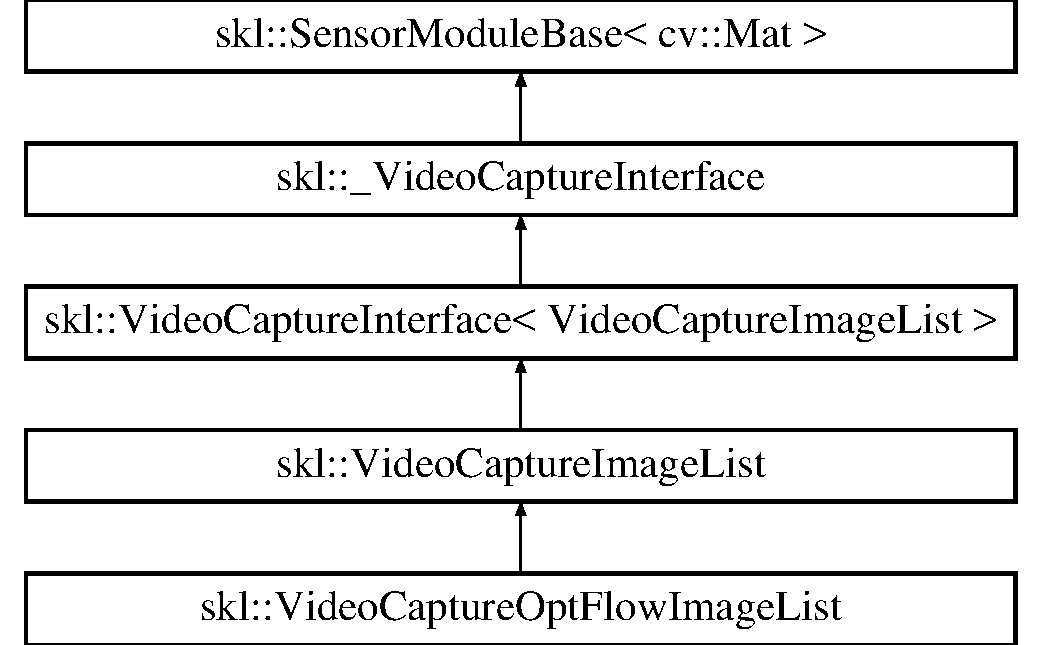
\includegraphics[height=5.000000cm]{classskl_1_1_video_capture_image_list}
\end{center}
\end{figure}
\subsection*{Public Member Functions}
\begin{DoxyCompactItemize}
\item 
\hypertarget{classskl_1_1_video_capture_image_list_a01adf7ae192e5c22ee43ff011f61aecb}{}\label{classskl_1_1_video_capture_image_list_a01adf7ae192e5c22ee43ff011f61aecb} 
\hyperlink{classskl_1_1_video_capture_image_list_a01adf7ae192e5c22ee43ff011f61aecb}{Video\+Capture\+Image\+List} ()
\begin{DoxyCompactList}\small\item\em デフォルトコンストラクタ \end{DoxyCompactList}\item 
\hypertarget{classskl_1_1_video_capture_image_list_afbd4271704c52c53c0044afc9554260e}{}\label{classskl_1_1_video_capture_image_list_afbd4271704c52c53c0044afc9554260e} 
virtual \hyperlink{classskl_1_1_video_capture_image_list_afbd4271704c52c53c0044afc9554260e}{$\sim$\+Video\+Capture\+Image\+List} ()
\begin{DoxyCompactList}\small\item\em デストラクタ \end{DoxyCompactList}\item 
\hypertarget{classskl_1_1_video_capture_image_list_ac2ee0961a1620389d30e367251cbc6fd}{}\label{classskl_1_1_video_capture_image_list_ac2ee0961a1620389d30e367251cbc6fd} 
virtual bool {\bfseries open} (const std\+::string \&filename)
\item 
\hypertarget{classskl_1_1_video_capture_image_list_a6ac572e50288fa2c48c6d48026124f46}{}\label{classskl_1_1_video_capture_image_list_a6ac572e50288fa2c48c6d48026124f46} 
bool {\bfseries is\+Opened} () const
\item 
\hypertarget{classskl_1_1_video_capture_image_list_aa341c3148f8cd67c152d8d24dc1c7a09}{}\label{classskl_1_1_video_capture_image_list_aa341c3148f8cd67c152d8d24dc1c7a09} 
void \hyperlink{classskl_1_1_video_capture_image_list_aa341c3148f8cd67c152d8d24dc1c7a09}{release} ()
\begin{DoxyCompactList}\small\item\em センサを特定する情報を入力する \end{DoxyCompactList}\item 
\hypertarget{classskl_1_1_video_capture_image_list_a6598af40f62a9088ee423aa966b77c09}{}\label{classskl_1_1_video_capture_image_list_a6598af40f62a9088ee423aa966b77c09} 
bool {\bfseries grab} ()
\item 
\hypertarget{classskl_1_1_video_capture_image_list_ab2291aa8a1dae8966a8f43716cb0d128}{}\label{classskl_1_1_video_capture_image_list_ab2291aa8a1dae8966a8f43716cb0d128} 
bool {\bfseries retrieve} (cv\+::\+Mat \&image, int channel=0)
\item 
\hypertarget{classskl_1_1_video_capture_image_list_ae7b49a05d26607c526c6f8082d15e979}{}\label{classskl_1_1_video_capture_image_list_ae7b49a05d26607c526c6f8082d15e979} 
virtual bool {\bfseries is\+Pseudo\+Capture} ()
\item 
\hypertarget{classskl_1_1_video_capture_image_list_acb500fb9f193ad0c0a94099426b4ebf9}{}\label{classskl_1_1_video_capture_image_list_acb500fb9f193ad0c0a94099426b4ebf9} 
bool \hyperlink{classskl_1_1_video_capture_image_list_acb500fb9f193ad0c0a94099426b4ebf9}{set} (capture\+\_\+property\+\_\+t prop\+\_\+id, double val)
\begin{DoxyCompactList}\small\item\em カメラに値やモード(camera\+\_\+mode\+\_\+tがset($\ast$,camera\+\_\+mode\+\_\+t mode)を通してvalに与えられる(modeは-\/4から-\/1までの整数)をセットする純粋仮想関数 \end{DoxyCompactList}\item 
\hypertarget{classskl_1_1_video_capture_image_list_a439231c580b1e93c68230667bfe07c1e}{}\label{classskl_1_1_video_capture_image_list_a439231c580b1e93c68230667bfe07c1e} 
double \hyperlink{classskl_1_1_video_capture_image_list_a439231c580b1e93c68230667bfe07c1e}{get} (capture\+\_\+property\+\_\+t prop\+\_\+id)
\begin{DoxyCompactList}\small\item\em カメラから値をgetする純粋仮想関数(modeはインターフェイス簡素化のためサポートしない) \end{DoxyCompactList}\end{DoxyCompactItemize}
\subsection*{Protected Member Functions}
\begin{DoxyCompactItemize}
\item 
\hypertarget{classskl_1_1_video_capture_image_list_aa520467fba47f993d72eac492ad34ad0}{}\label{classskl_1_1_video_capture_image_list_aa520467fba47f993d72eac492ad34ad0} 
void {\bfseries generate\+Index} (const std\+::vector$<$ std\+::string $>$ \&list, std\+::vector$<$ std\+::pair$<$ size\+\_\+t, bool $>$ $>$ \&index)
\end{DoxyCompactItemize}
\subsection*{Protected Attributes}
\begin{DoxyCompactItemize}
\item 
\hypertarget{classskl_1_1_video_capture_image_list_a07a9d7ba42284858346a0b22f79a8546}{}\label{classskl_1_1_video_capture_image_list_a07a9d7ba42284858346a0b22f79a8546} 
int {\bfseries index}
\item 
\hypertarget{classskl_1_1_video_capture_image_list_aa45d84456af4dd8819cd5a1248346659}{}\label{classskl_1_1_video_capture_image_list_aa45d84456af4dd8819cd5a1248346659} 
std\+::vector$<$ std\+::pair$<$ size\+\_\+t, bool $>$ $>$ {\bfseries img\+\_\+list}
\item 
\hypertarget{classskl_1_1_video_capture_image_list_afc70915373577ee01bb546f3b6792075}{}\label{classskl_1_1_video_capture_image_list_afc70915373577ee01bb546f3b6792075} 
std\+::vector$<$ std\+::string $>$ {\bfseries img\+\_\+list\+\_\+}
\item 
\hypertarget{classskl_1_1_video_capture_image_list_ada19dc79dc7bf69d12c91735db419e8a}{}\label{classskl_1_1_video_capture_image_list_ada19dc79dc7bf69d12c91735db419e8a} 
int {\bfseries bayer\+\_\+change}
\item 
\hypertarget{classskl_1_1_video_capture_image_list_abb1a3688f5789ccb88e1f813d31237bb}{}\label{classskl_1_1_video_capture_image_list_abb1a3688f5789ccb88e1f813d31237bb} 
int {\bfseries imread\+\_\+option}
\item 
\hypertarget{classskl_1_1_video_capture_image_list_aca89f798845c8da4039c032705a79953}{}\label{classskl_1_1_video_capture_image_list_aca89f798845c8da4039c032705a79953} 
int {\bfseries checked\+\_\+frame\+\_\+pos}
\end{DoxyCompactItemize}


\subsection{Detailed Description}
画像列が記述されたファイルリストからファイルを読み込む 

The documentation for this class was generated from the following files\+:\begin{DoxyCompactItemize}
\item 
Open\+C\+V/include/\hyperlink{_video_capture_image_list_8h}{Video\+Capture\+Image\+List.\+h}\item 
Open\+C\+V/src/\hyperlink{_video_capture_image_list_8cpp}{Video\+Capture\+Image\+List.\+cpp}\end{DoxyCompactItemize}

\hypertarget{classskl_1_1_video_capture_interface}{}\section{skl\+:\+:Video\+Capture\+Interface$<$ T $>$ Class Template Reference}
\label{classskl_1_1_video_capture_interface}\index{skl\+::\+Video\+Capture\+Interface$<$ T $>$@{skl\+::\+Video\+Capture\+Interface$<$ T $>$}}


S\+K\+Lにおける\+Video\+Capture用のインターフェイス(operator$>$$>$つき)  




{\ttfamily \#include $<$Video\+Capture\+Interface.\+h$>$}

Inheritance diagram for skl\+:\+:Video\+Capture\+Interface$<$ T $>$\+:\begin{figure}[H]
\begin{center}
\leavevmode
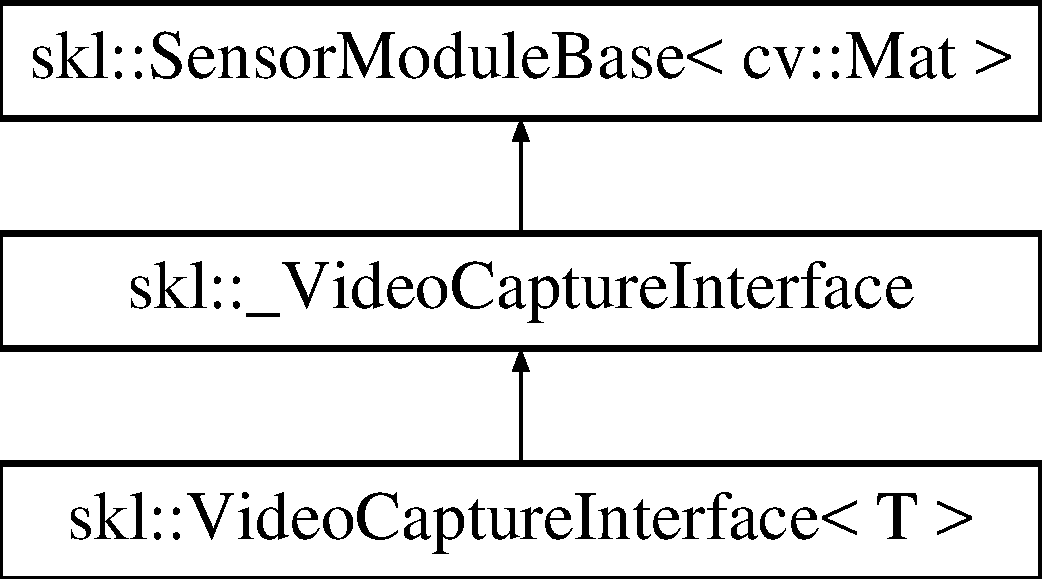
\includegraphics[height=3.000000cm]{classskl_1_1_video_capture_interface}
\end{center}
\end{figure}
\subsection*{Public Member Functions}
\begin{DoxyCompactItemize}
\item 
\hypertarget{classskl_1_1_video_capture_interface_ac4a2788a79f8a4a3382467e5fa67f128}{}\label{classskl_1_1_video_capture_interface_ac4a2788a79f8a4a3382467e5fa67f128} 
virtual T \& {\bfseries operator$>$$>$} (cv\+::\+Mat \&image)
\end{DoxyCompactItemize}
\subsection*{Additional Inherited Members}


\subsection{Detailed Description}
\subsubsection*{template$<$class T$>$\newline
class skl\+::\+Video\+Capture\+Interface$<$ T $>$}

S\+K\+Lにおける\+Video\+Capture用のインターフェイス(operator$>$$>$つき) 

The documentation for this class was generated from the following file\+:\begin{DoxyCompactItemize}
\item 
Open\+C\+V/include/\hyperlink{_video_capture_interface_8h}{Video\+Capture\+Interface.\+h}\end{DoxyCompactItemize}

\hypertarget{classskl_1_1_video_capture_opt_flow_image_list}{}\section{skl\+:\+:Video\+Capture\+Opt\+Flow\+Image\+List Class Reference}
\label{classskl_1_1_video_capture_opt_flow_image_list}\index{skl\+::\+Video\+Capture\+Opt\+Flow\+Image\+List@{skl\+::\+Video\+Capture\+Opt\+Flow\+Image\+List}}


オプティカルフローとして得られた32\+F\+C1の行列からなる\+Image\+Listを読み出すための関数  




{\ttfamily \#include $<$Video\+Capture\+Opt\+Flow\+Image\+List.\+h$>$}

Inheritance diagram for skl\+:\+:Video\+Capture\+Opt\+Flow\+Image\+List\+:\begin{figure}[H]
\begin{center}
\leavevmode
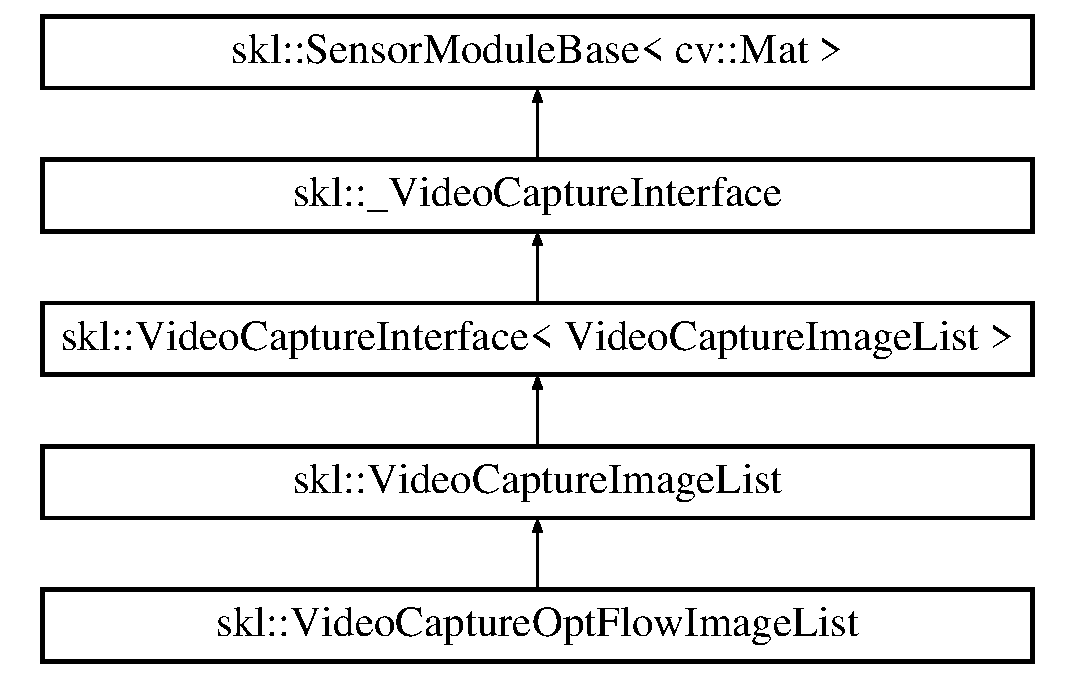
\includegraphics[height=5.000000cm]{classskl_1_1_video_capture_opt_flow_image_list}
\end{center}
\end{figure}
\subsection*{Public Member Functions}
\begin{DoxyCompactItemize}
\item 
\hypertarget{classskl_1_1_video_capture_opt_flow_image_list_a36b0491c64fd43719187d2ac52336949}{}\label{classskl_1_1_video_capture_opt_flow_image_list_a36b0491c64fd43719187d2ac52336949} 
\hyperlink{classskl_1_1_video_capture_opt_flow_image_list_a36b0491c64fd43719187d2ac52336949}{Video\+Capture\+Opt\+Flow\+Image\+List} ()
\begin{DoxyCompactList}\small\item\em デフォルトコンストラクタ \end{DoxyCompactList}\item 
\hypertarget{classskl_1_1_video_capture_opt_flow_image_list_aea727356fa14b01db10452bc72600fd2}{}\label{classskl_1_1_video_capture_opt_flow_image_list_aea727356fa14b01db10452bc72600fd2} 
virtual \hyperlink{classskl_1_1_video_capture_opt_flow_image_list_aea727356fa14b01db10452bc72600fd2}{$\sim$\+Video\+Capture\+Opt\+Flow\+Image\+List} ()
\begin{DoxyCompactList}\small\item\em デストラクタ \end{DoxyCompactList}\item 
\hypertarget{classskl_1_1_video_capture_opt_flow_image_list_afdf96b1882e6da453316a6af28ef3a96}{}\label{classskl_1_1_video_capture_opt_flow_image_list_afdf96b1882e6da453316a6af28ef3a96} 
bool {\bfseries open} (const std\+::string \&filename)
\item 
\hypertarget{classskl_1_1_video_capture_opt_flow_image_list_a71e22f4c62b46802043d57ecd37afc03}{}\label{classskl_1_1_video_capture_opt_flow_image_list_a71e22f4c62b46802043d57ecd37afc03} 
bool {\bfseries grab} ()
\item 
\hypertarget{classskl_1_1_video_capture_opt_flow_image_list_aa4123850509f5dd63feb04e6309c207c}{}\label{classskl_1_1_video_capture_opt_flow_image_list_aa4123850509f5dd63feb04e6309c207c} 
bool {\bfseries retrieve} (cv\+::\+Mat \&image, int channel=1)
\end{DoxyCompactItemize}
\subsection*{Protected Attributes}
\begin{DoxyCompactItemize}
\item 
\hypertarget{classskl_1_1_video_capture_opt_flow_image_list_a74e6b99f2dbdd7ae12fe78e4c4bb2a6e}{}\label{classskl_1_1_video_capture_opt_flow_image_list_a74e6b99f2dbdd7ae12fe78e4c4bb2a6e} 
\hyperlink{classskl_1_1_flow}{Flow} {\bfseries flow}
\item 
\hypertarget{classskl_1_1_video_capture_opt_flow_image_list_ace9bb1949e08282fdb0e3a153e8329b2}{}\label{classskl_1_1_video_capture_opt_flow_image_list_ace9bb1949e08282fdb0e3a153e8329b2} 
bool {\bfseries has\+Flow}
\end{DoxyCompactItemize}
\subsection*{Additional Inherited Members}


\subsection{Detailed Description}
オプティカルフローとして得られた32\+F\+C1の行列からなる\+Image\+Listを読み出すための関数 

The documentation for this class was generated from the following files\+:\begin{DoxyCompactItemize}
\item 
Open\+C\+V/include/\hyperlink{_video_capture_opt_flow_image_list_8h}{Video\+Capture\+Opt\+Flow\+Image\+List.\+h}\item 
Open\+C\+V/src/\hyperlink{_video_capture_opt_flow_image_list_8cpp}{Video\+Capture\+Opt\+Flow\+Image\+List.\+cpp}\end{DoxyCompactItemize}

\hypertarget{classskl_1_1_video_capture_params}{}\section{skl\+:\+:Video\+Capture\+Params Class Reference}
\label{classskl_1_1_video_capture_params}\index{skl\+::\+Video\+Capture\+Params@{skl\+::\+Video\+Capture\+Params}}


Video\+Captureクラスの取るパラメタをあらわす値オブジェクト  




{\ttfamily \#include $<$Video\+Capture\+Params.\+h$>$}

Inheritance diagram for skl\+:\+:Video\+Capture\+Params\+:\begin{figure}[H]
\begin{center}
\leavevmode
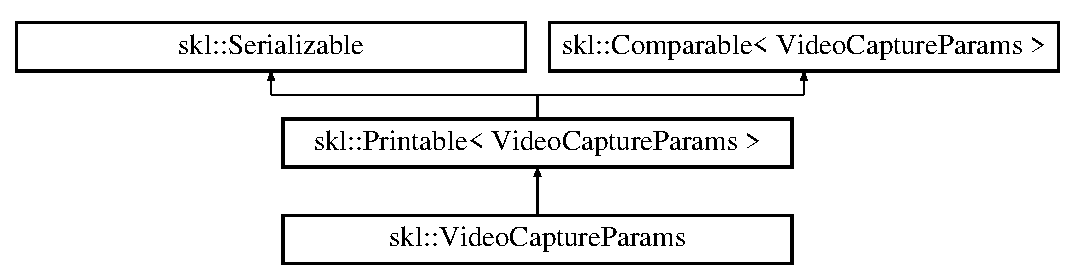
\includegraphics[height=3.000000cm]{classskl_1_1_video_capture_params}
\end{center}
\end{figure}
\subsection*{Public Member Functions}
\begin{DoxyCompactItemize}
\item 
\hypertarget{classskl_1_1_video_capture_params_af40b080bb9b67de7fcf94669d66cbf96}{}\label{classskl_1_1_video_capture_params_af40b080bb9b67de7fcf94669d66cbf96} 
\hyperlink{classskl_1_1_video_capture_params_af40b080bb9b67de7fcf94669d66cbf96}{Video\+Capture\+Params} ()
\begin{DoxyCompactList}\small\item\em デフォルトコンストラクタ \end{DoxyCompactList}\item 
\hypertarget{classskl_1_1_video_capture_params_aacbd136b60504c7955c2b959a130e82b}{}\label{classskl_1_1_video_capture_params_aacbd136b60504c7955c2b959a130e82b} 
virtual \hyperlink{classskl_1_1_video_capture_params_aacbd136b60504c7955c2b959a130e82b}{$\sim$\+Video\+Capture\+Params} ()
\begin{DoxyCompactList}\small\item\em デストラクタ \end{DoxyCompactList}\item 
\hypertarget{classskl_1_1_video_capture_params_a83bf21e7cadfc5457acfd5263f17e48a}{}\label{classskl_1_1_video_capture_params_a83bf21e7cadfc5457acfd5263f17e48a} 
{\bfseries Video\+Capture\+Params} (const std\+::string \&filename)
\item 
\hypertarget{classskl_1_1_video_capture_params_a29693a80e5194706ef86ccbf4d10a6a4}{}\label{classskl_1_1_video_capture_params_a29693a80e5194706ef86ccbf4d10a6a4} 
{\bfseries Video\+Capture\+Params} (const \hyperlink{classskl_1_1_video_capture_params}{Video\+Capture\+Params} \&other)
\item 
\hypertarget{classskl_1_1_video_capture_params_a2f508d9369b30d5a451fb5474d4ecf0d}{}\label{classskl_1_1_video_capture_params_a2f508d9369b30d5a451fb5474d4ecf0d} 
std\+::string {\bfseries print} () const
\item 
\hypertarget{classskl_1_1_video_capture_params_a3b6da0a862221ccd00540bdf30d3e52f}{}\label{classskl_1_1_video_capture_params_a3b6da0a862221ccd00540bdf30d3e52f} 
bool {\bfseries scan} (const std\+::string \&\hyperlink{classskl_1_1_serializable_a1d203d9f0049ce37183a0dcefbc6399a}{buf})
\item 
\hypertarget{classskl_1_1_video_capture_params_a3175df1d5cd95ea440af4bac2ef1fcc4}{}\label{classskl_1_1_video_capture_params_a3175df1d5cd95ea440af4bac2ef1fcc4} 
bool {\bfseries load} (const std\+::string \&filename)
\item 
\hypertarget{classskl_1_1_video_capture_params_a32e66835b685c54a8e7f5a8fc6e9c8cc}{}\label{classskl_1_1_video_capture_params_a32e66835b685c54a8e7f5a8fc6e9c8cc} 
void {\bfseries save} (const std\+::string \&filename) const
\item 
\hypertarget{classskl_1_1_video_capture_params_ae44da21ef359988122f3fb6025e4a8e1}{}\label{classskl_1_1_video_capture_params_ae44da21ef359988122f3fb6025e4a8e1} 
bool {\bfseries set} (const std\+::string \&prop\+\_\+name, double val)
\item 
\hypertarget{classskl_1_1_video_capture_params_aab28c742742f07298daeccc69f1f5c5a}{}\label{classskl_1_1_video_capture_params_aab28c742742f07298daeccc69f1f5c5a} 
bool {\bfseries set} (capture\+\_\+property\+\_\+t prop\+\_\+id, double val)
\item 
\hypertarget{classskl_1_1_video_capture_params_ac56658132ec7f52191fb2472cf98722e}{}\label{classskl_1_1_video_capture_params_ac56658132ec7f52191fb2472cf98722e} 
double {\bfseries get} (const std\+::string \&prop\+\_\+name) const
\item 
\hypertarget{classskl_1_1_video_capture_params_aee1237be209c4fc391d6b669b12e3da9}{}\label{classskl_1_1_video_capture_params_aee1237be209c4fc391d6b669b12e3da9} 
double {\bfseries get} (capture\+\_\+property\+\_\+t prop\+\_\+id) const
\item 
\hypertarget{classskl_1_1_video_capture_params_a1ee73f1fa13bafbc81983f2ddc785900}{}\label{classskl_1_1_video_capture_params_a1ee73f1fa13bafbc81983f2ddc785900} 
Video\+Capture\+Param\+Iter {\bfseries begin} () const
\item 
\hypertarget{classskl_1_1_video_capture_params_aaa6f72614c3f0cda98cb317fae7661cb}{}\label{classskl_1_1_video_capture_params_aaa6f72614c3f0cda98cb317fae7661cb} 
Video\+Capture\+Param\+Iter {\bfseries end} () const
\item 
\hypertarget{classskl_1_1_video_capture_params_a2349d10365509e2ea4b8fa973b241c76}{}\label{classskl_1_1_video_capture_params_a2349d10365509e2ea4b8fa973b241c76} 
const std\+::map$<$ std\+::string, capture\+\_\+property\+\_\+t $>$ \& {\bfseries get\+Property\+Name\+I\+D\+Map} ()
\end{DoxyCompactItemize}
\subsection*{Protected Attributes}
\begin{DoxyCompactItemize}
\item 
\hypertarget{classskl_1_1_video_capture_params_a0a782d9ebee1e922da5245d776a224d8}{}\label{classskl_1_1_video_capture_params_a0a782d9ebee1e922da5245d776a224d8} 
std\+::map$<$ capture\+\_\+property\+\_\+t, double $>$ {\bfseries property\+\_\+id\+\_\+value\+\_\+map}
\end{DoxyCompactItemize}
\subsection*{Static Protected Attributes}
\begin{DoxyCompactItemize}
\item 
\hypertarget{classskl_1_1_video_capture_params_adf62f7037731cc3085a036fbe2ed5b06}{}\label{classskl_1_1_video_capture_params_adf62f7037731cc3085a036fbe2ed5b06} 
static std\+::map$<$ std\+::string, capture\+\_\+property\+\_\+t $>$ {\bfseries property\+\_\+name\+\_\+id\+\_\+map}
\end{DoxyCompactItemize}
\subsection*{Friends}
\begin{DoxyCompactItemize}
\item 
\hypertarget{classskl_1_1_video_capture_params_a05c26b898da174ea1187ea51676f2517}{}\label{classskl_1_1_video_capture_params_a05c26b898da174ea1187ea51676f2517} 
class {\bfseries Video\+Param\+Adder}
\end{DoxyCompactItemize}
\subsection*{Additional Inherited Members}


\subsection{Detailed Description}
Video\+Captureクラスの取るパラメタをあらわす値オブジェクト 

The documentation for this class was generated from the following files\+:\begin{DoxyCompactItemize}
\item 
Open\+C\+V/include/\hyperlink{_video_capture_params_8h}{Video\+Capture\+Params.\+h}\item 
Open\+C\+V/src/\hyperlink{_video_capture_params_8cpp}{Video\+Capture\+Params.\+cpp}\end{DoxyCompactItemize}

\hypertarget{class_xE6_x8E_xA5_xE8_xA7_xA6_xE7_x90_x86_xE7_x94_xB1_xE4_xBB_x98_xE3_x81_x91_xE3_x82_x92_xE5_x890112ad43302b940b72aaba1c07dd87f}{}\section{接触理由付けを利用した机上物体検出 Class Reference}
\label{class_xE6_x8E_xA5_xE8_xA7_xA6_xE7_x90_x86_xE7_x94_xB1_xE4_xBB_x98_xE3_x81_x91_xE3_x82_x92_xE5_x890112ad43302b940b72aaba1c07dd87f}\index{接触理由付けを利用した机上物体検出@{接触理由付けを利用した机上物体検出}}


The documentation for this class was generated from the following file\+:\begin{DoxyCompactItemize}
\item 
Open\+C\+V\+G\+P\+U/include/Table\+Object\+Manager\+With\+Touch\+Reasoning\+Gpu.\+h\end{DoxyCompactItemize}

\hypertarget{class_xE6_x8E_xA5_xE8_xA7_xA6_xE7_x90_x86_xE7_x94_xB1_xE4_xBB_x98_xE3_x81_x91_xE3_x82_x92_xE7_x94_xA8_xE3_x81_x84_xE3_x81_x9F}{}\section{接触理由付けを用いた Class Reference}
\label{class_xE6_x8E_xA5_xE8_xA7_xA6_xE7_x90_x86_xE7_x94_xB1_xE4_xBB_x98_xE3_x81_x91_xE3_x82_x92_xE7_x94_xA8_xE3_x81_x84_xE3_x81_x9F}\index{接触理由付けを用いた@{接触理由付けを用いた}}


The documentation for this class was generated from the following file\+:\begin{DoxyCompactItemize}
\item 
Open\+C\+V/include/\hyperlink{_table_object_manager_with_touch_reasoning_8h}{Table\+Object\+Manager\+With\+Touch\+Reasoning.\+h}\end{DoxyCompactItemize}

\hypertarget{class_xE6_x9C_xBA_xE4_xB8_x8A_xE7_x89_xA9_xE4_xBD_x93_xE3_x81_xAE_xE7_x8A_xB6_xE6_x85_x8B_xE3_x8db069bd01051f325aba399d9080d849d}{}\section{机上物体の状態を保持する値型オブジェクト Class Reference}
\label{class_xE6_x9C_xBA_xE4_xB8_x8A_xE7_x89_xA9_xE4_xBD_x93_xE3_x81_xAE_xE7_x8A_xB6_xE6_x85_x8B_xE3_x8db069bd01051f325aba399d9080d849d}\index{机上物体の状態を保持する値型オブジェクト@{机上物体の状態を保持する値型オブジェクト}}


{\ttfamily \#include $<$Object\+State.\+h$>$}



\subsection{Detailed Description}
\begin{DoxyNote}{Note}
得に意味的なつながりは無いが、データ構造が似ているのでオプティカルフロークラスを継承して関数を流用 
\end{DoxyNote}


The documentation for this class was generated from the following file\+:\begin{DoxyCompactItemize}
\item 
Open\+C\+V/include/\hyperlink{_object_state_8h}{Object\+State.\+h}\end{DoxyCompactItemize}

\hypertarget{class_xE9_xAB_x98_xE9_x80_x9F_xE3_x81_xAB2_xE3_x83_x95_xE3_x83_xAC_xE3_x83_xBC_xE3_x83_xA0_xE9_xe53c8fde8d63a4cabd051bddcffbadf5}{}\section{高速に2フレーム間で動きがあるかどうかをチェックする Class Reference}
\label{class_xE9_xAB_x98_xE9_x80_x9F_xE3_x81_xAB2_xE3_x83_x95_xE3_x83_xAC_xE3_x83_xBC_xE3_x83_xA0_xE9_xe53c8fde8d63a4cabd051bddcffbadf5}\index{高速に2フレーム間で動きがあるかどうかをチェックする@{高速に2フレーム間で動きがあるかどうかをチェックする}}


The documentation for this class was generated from the following file\+:\begin{DoxyCompactItemize}
\item 
Open\+C\+V/include/Count\+Moving\+Pixels.\+h\end{DoxyCompactItemize}

\chapter{File Documentation}
\hypertarget{_chiffon_base_8h}{}\section{Core/include/\+Chiffon\+Base.h File Reference}
\label{_chiffon_base_8h}\index{Core/include/\+Chiffon\+Base.\+h@{Core/include/\+Chiffon\+Base.\+h}}
{\ttfamily \#include \char`\"{}picojson/picojson.\+h\char`\"{}}\newline
{\ttfamily \#include \char`\"{}H\+T\+T\+P\+Client.\+h\char`\"{}}\newline
\subsection*{Classes}
\begin{DoxyCompactItemize}
\item 
class \hyperlink{classskl_1_1_chiffon_base}{skl\+::\+Chiffon\+Base}
\begin{DoxyCompactList}\small\item\em Chiffon\+Vieer/\+Navigator共通の処理を記述するインターフェイス  \end{DoxyCompactList}\end{DoxyCompactItemize}


\subsection{Detailed Description}
\begin{DoxyAuthor}{Author}
kitchen 
\end{DoxyAuthor}
\begin{DoxyDate}{Date}
Date Created\+: 2015/\+Feb/07 

Last Change\+:2015/\+Feb/07. 
\end{DoxyDate}

\hypertarget{_comparable_8h}{}\section{Core/include/\+Comparable.h File Reference}
\label{_comparable_8h}\index{Core/include/\+Comparable.\+h@{Core/include/\+Comparable.\+h}}
\subsection*{Classes}
\begin{DoxyCompactItemize}
\item 
class \hyperlink{classskl_1_1_comparable}{skl\+::\+Comparable$<$ T $>$}
\begin{DoxyCompactList}\small\item\em 比較可能なオブジェクトであることを示す(operator$<$を定義するだけで他の比較演算子が出来る) \end{DoxyCompactList}\end{DoxyCompactItemize}


\subsection{Detailed Description}
\begin{DoxyAuthor}{Author}
橋本敦史 
\end{DoxyAuthor}
\begin{DoxyDate}{Date}
Last Change\+:2012/\+Jan/06. 
\end{DoxyDate}

\hypertarget{_filter_8h}{}\section{Core/include/\+Filter.h File Reference}
\label{_filter_8h}\index{Core/include/\+Filter.\+h@{Core/include/\+Filter.\+h}}
\subsection*{Classes}
\begin{DoxyCompactItemize}
\item 
class \hyperlink{classskl_1_1___filter}{skl\+::\+\_\+\+Filter$<$ R\+E\+T, S\+R\+C, D\+I\+S\+T $>$}
\begin{DoxyCompactList}\small\item\em compute関数を持っているクラスであることを保証するインターフェイス \end{DoxyCompactList}\end{DoxyCompactItemize}


\subsection{Detailed Description}
\begin{DoxyAuthor}{Author}
a\+\_\+hasimoto 
\end{DoxyAuthor}
\begin{DoxyDate}{Date}
Date Created\+: 2012/\+Feb/10 

Last Change\+:2012/\+May/22. 
\end{DoxyDate}

\hypertarget{_h_t_t_p_client_8h}{}\section{Core/include/\+H\+T\+T\+P\+Client.h File Reference}
\label{_h_t_t_p_client_8h}\index{Core/include/\+H\+T\+T\+P\+Client.\+h@{Core/include/\+H\+T\+T\+P\+Client.\+h}}
{\ttfamily \#include $<$boost/asio.\+hpp$>$}\newline
{\ttfamily \#include \char`\"{}skl.\+h\char`\"{}}\newline
\subsection*{Classes}
\begin{DoxyCompactItemize}
\item 
class \hyperlink{classskl_1_1_h_t_t_p_client}{skl\+::\+H\+T\+T\+P\+Client}
\begin{DoxyCompactList}\small\item\em \hyperlink{classskl_1_1_h_t_t_p_client}{H\+T\+T\+P\+Client} get/post requestを送るクラス(redirectには対応していない簡単なもの) \end{DoxyCompactList}\item 
class \hyperlink{classskl_1_1_h_t_t_p_client_1_1tcp__client}{skl\+::\+H\+T\+T\+P\+Client\+::tcp\+\_\+client}
\end{DoxyCompactItemize}


\subsection{Detailed Description}
\begin{DoxyAuthor}{Author}
kitchen 
\end{DoxyAuthor}
\begin{DoxyDate}{Date}
Date Created\+: 2015/\+Feb/07 

Last Change\+:2015/\+Feb/07. 
\end{DoxyDate}

\hypertarget{_key_input_8h}{}\section{Core/include/\+Key\+Input.h File Reference}
\label{_key_input_8h}\index{Core/include/\+Key\+Input.\+h@{Core/include/\+Key\+Input.\+h}}
{\ttfamily \#include $<$string$>$}\newline
{\ttfamily \#include $<$sstream$>$}\newline
\subsection*{Classes}
\begin{DoxyCompactItemize}
\item 
class \hyperlink{classskl_1_1_key_input}{skl\+::\+Key\+Input}
\end{DoxyCompactItemize}


\subsection{Detailed Description}
\begin{DoxyAuthor}{Author}
橋本敦史 
\end{DoxyAuthor}
\begin{DoxyDate}{Date}
Last Change\+:2012/\+Oct/14. 
\end{DoxyDate}

\hypertarget{_opt_parser_8h}{}\section{Core/include/\+Opt\+Parser.h File Reference}
\label{_opt_parser_8h}\index{Core/include/\+Opt\+Parser.\+h@{Core/include/\+Opt\+Parser.\+h}}
{\ttfamily \#include $<$map$>$}\newline
{\ttfamily \#include $<$vector$>$}\newline
{\ttfamily \#include $<$string$>$}\newline
{\ttfamily \#include $<$sstream$>$}\newline
{\ttfamily \#include $<$algorithm$>$}\newline
{\ttfamily \#include $<$cassert$>$}\newline
{\ttfamily \#include \char`\"{}sklstring.\+h\char`\"{}}\newline
\subsection*{Classes}
\begin{DoxyCompactItemize}
\item 
class \hyperlink{classskl_1_1_opt_parser}{skl\+::\+Opt\+Parser}
\begin{DoxyCompactList}\small\item\em Parse Option from Command\+Line. \end{DoxyCompactList}\item 
class \hyperlink{classskl_1_1_opt_parser_atom_interface}{skl\+::\+Opt\+Parser\+Atom\+Interface}
\item 
class \hyperlink{classskl_1_1_opt_parser_atom}{skl\+::\+Opt\+Parser\+Atom$<$ T $>$}
\item 
class \hyperlink{classskl_1_1_opt_parser_atom_container}{skl\+::\+Opt\+Parser\+Atom\+Container$<$ T, Container $>$}
\end{DoxyCompactItemize}
\subsection*{Macros}
\begin{DoxyCompactItemize}
\item 
\hypertarget{_opt_parser_8h_a4ea405037f37641df90239d0f3767fcf}{}\label{_opt_parser_8h_a4ea405037f37641df90239d0f3767fcf} 
\#define {\bfseries opt\+\_\+on\+\_\+bool}(V\+AR,  S\+H\+O\+R\+T\+\_\+\+F\+O\+RM,  E\+X\+P\+L\+A\+N\+A\+T\+I\+ON)~opt\+\_\+on(bool, V\+AR, false, S\+H\+O\+R\+T\+\_\+\+F\+O\+RM, \char`\"{}$<$B\+O\+OL$>$\char`\"{}, E\+X\+P\+L\+A\+N\+A\+T\+I\+ON)
\item 
\#define {\bfseries opt\+\_\+on}(T\+Y\+PE,  V\+AR,  D\+E\+F\+A\+U\+L\+T\+\_\+\+V\+AL,  S\+H\+O\+R\+T\+\_\+\+F\+O\+RM,  E\+X\+P\+R\+E\+S\+S\+I\+ON,  E\+X\+P\+L\+A\+N\+A\+T\+I\+ON)
\item 
\#define {\bfseries opt\+\_\+on\+\_\+container}(C\+O\+N\+T\+A\+I\+N\+E\+R\+\_\+\+T\+Y\+PE,  E\+L\+E\+M\+\_\+\+T\+Y\+PE,  V\+AR,  D\+E\+F\+A\+U\+L\+T\+\_\+\+V\+AL,  S\+H\+O\+R\+T\+\_\+\+F\+O\+RM,  E\+X\+P\+R\+E\+S\+S\+I\+ON,  E\+X\+P\+L\+A\+N\+A\+T\+I\+ON,  D\+E\+L\+I\+M\+I\+N\+A\+T\+OR,  L\+E\+N\+G\+TH)
\item 
\#define {\bfseries opt\+\_\+parse}(P\+A\+R\+S\+ER,  A\+R\+GC,  A\+R\+GV,  A\+R\+GS)
\item 
\hypertarget{_opt_parser_8h_a103fe6e979af6382db35faa05562f007}{}\label{_opt_parser_8h_a103fe6e979af6382db35faa05562f007} 
\#define {\bfseries generate\+\_\+atomic\+\_\+parser}(T\+Y\+PE,  V\+AR,  S\+H\+O\+R\+T\+\_\+\+F\+O\+RM,  E\+X\+P\+R\+E\+S\+S\+I\+ON,  E\+X\+P\+L\+A\+N\+A\+T\+I\+ON)~\hyperlink{classskl_1_1_opt_parser_atom}{skl\+::\+Opt\+Parser\+Atom}$<$T\+Y\+PE$>$ \+\_\+\+\_\+opt\+\_\+parser\+\_\+atom\+\_\+\#\#V\+AR(S\+H\+O\+R\+T\+\_\+\+F\+O\+RM, \#V\+AR, E\+X\+P\+R\+E\+S\+S\+I\+ON, E\+X\+P\+L\+A\+N\+A\+T\+I\+ON, \&V\+AR)
\item 
\hypertarget{_opt_parser_8h_af0ef192a29ced2928675e3b334a71ac3}{}\label{_opt_parser_8h_af0ef192a29ced2928675e3b334a71ac3} 
\#define {\bfseries generate\+\_\+atomic\+\_\+parser\+\_\+container}(C\+O\+N\+T\+A\+I\+N\+E\+R\+\_\+\+T\+Y\+PE,  E\+L\+E\+M\+\_\+\+T\+Y\+PE,  V\+AR,  D\+E\+F\+A\+U\+L\+T\+\_\+\+V\+AL,  S\+H\+O\+R\+T\+\_\+\+F\+O\+RM,  E\+X\+P\+R\+E\+S\+S\+I\+ON,  E\+X\+P\+L\+A\+N\+A\+T\+I\+ON,  D\+E\+L\+I\+M\+I\+N\+A\+T\+OR,  L\+E\+N\+G\+TH)~\hyperlink{classskl_1_1_opt_parser_atom_container}{skl\+::\+Opt\+Parser\+Atom\+Container} $<$ E\+L\+E\+M\+\_\+\+T\+Y\+PE, C\+O\+N\+T\+A\+I\+N\+E\+R\+\_\+\+T\+Y\+PE $<$ E\+L\+E\+M\+\_\+\+T\+Y\+PE $>$ $>$ \+\_\+\+\_\+opt\+\_\+parser\+\_\+atom\+\_\+container\+\_\+\#\#V\+AR(S\+H\+O\+R\+T\+\_\+\+F\+O\+RM, \#V\+AR, D\+E\+F\+A\+U\+L\+T\+\_\+\+V\+AL, E\+X\+P\+R\+E\+S\+S\+I\+ON, E\+X\+P\+L\+A\+N\+A\+T\+I\+ON, \&V\+AR, D\+E\+L\+I\+M\+I\+N\+A\+T\+OR, L\+E\+N\+G\+TH)
\end{DoxyCompactItemize}


\subsection{Detailed Description}
\begin{DoxyAuthor}{Author}
a\+\_\+hasimoto 
\end{DoxyAuthor}
\begin{DoxyDate}{Date}
Date Created\+: 2011/\+Dec/27 

Last Change\+:2013/\+Nov/25. 
\end{DoxyDate}


\subsection{Macro Definition Documentation}
\hypertarget{_opt_parser_8h_a5d8d40ef669f167dc209c128efc3e704}{}\label{_opt_parser_8h_a5d8d40ef669f167dc209c128efc3e704} 
\index{Opt\+Parser.\+h@{Opt\+Parser.\+h}!opt\+\_\+on@{opt\+\_\+on}}
\index{opt\+\_\+on@{opt\+\_\+on}!Opt\+Parser.\+h@{Opt\+Parser.\+h}}
\subsubsection{\texorpdfstring{opt\+\_\+on}{opt\_on}}
{\footnotesize\ttfamily \#define opt\+\_\+on(\begin{DoxyParamCaption}\item[{}]{T\+Y\+PE,  }\item[{}]{V\+AR,  }\item[{}]{D\+E\+F\+A\+U\+L\+T\+\_\+\+V\+AL,  }\item[{}]{S\+H\+O\+R\+T\+\_\+\+F\+O\+RM,  }\item[{}]{E\+X\+P\+R\+E\+S\+S\+I\+ON,  }\item[{}]{E\+X\+P\+L\+A\+N\+A\+T\+I\+ON }\end{DoxyParamCaption})}

{\bfseries Value\+:}
\begin{DoxyCode}
TYPE VAR( DEFAULT\_VAL );\(\backslash\)
generate\_atomic\_parser(TYPE,VAR,SHORT\_FORM, EXPRESSION, EXPLANATION);\(\backslash\)
\end{DoxyCode}
\hypertarget{_opt_parser_8h_abe64775ae9a5b782eec45cf9425c582b}{}\label{_opt_parser_8h_abe64775ae9a5b782eec45cf9425c582b} 
\index{Opt\+Parser.\+h@{Opt\+Parser.\+h}!opt\+\_\+on\+\_\+container@{opt\+\_\+on\+\_\+container}}
\index{opt\+\_\+on\+\_\+container@{opt\+\_\+on\+\_\+container}!Opt\+Parser.\+h@{Opt\+Parser.\+h}}
\subsubsection{\texorpdfstring{opt\+\_\+on\+\_\+container}{opt\_on\_container}}
{\footnotesize\ttfamily \#define opt\+\_\+on\+\_\+container(\begin{DoxyParamCaption}\item[{}]{C\+O\+N\+T\+A\+I\+N\+E\+R\+\_\+\+T\+Y\+PE,  }\item[{}]{E\+L\+E\+M\+\_\+\+T\+Y\+PE,  }\item[{}]{V\+AR,  }\item[{}]{D\+E\+F\+A\+U\+L\+T\+\_\+\+V\+AL,  }\item[{}]{S\+H\+O\+R\+T\+\_\+\+F\+O\+RM,  }\item[{}]{E\+X\+P\+R\+E\+S\+S\+I\+ON,  }\item[{}]{E\+X\+P\+L\+A\+N\+A\+T\+I\+ON,  }\item[{}]{D\+E\+L\+I\+M\+I\+N\+A\+T\+OR,  }\item[{}]{L\+E\+N\+G\+TH }\end{DoxyParamCaption})}

{\bfseries Value\+:}
\begin{DoxyCode}
CONTAINER\_TYPE< ELEM\_TYPE > VAR;\(\backslash\)
generate\_atomic\_parser\_container(CONTAINER\_TYPE, ELEM\_TYPE,VAR,DEFAULT\_VAL, SHORT\_FORM, EXPRESSION, 
      EXPLANATION, DELIMINATOR, LENGTH);\(\backslash\)
\end{DoxyCode}
\hypertarget{_opt_parser_8h_a309d3f15951f807bf7493c18670ef755}{}\label{_opt_parser_8h_a309d3f15951f807bf7493c18670ef755} 
\index{Opt\+Parser.\+h@{Opt\+Parser.\+h}!opt\+\_\+parse@{opt\+\_\+parse}}
\index{opt\+\_\+parse@{opt\+\_\+parse}!Opt\+Parser.\+h@{Opt\+Parser.\+h}}
\subsubsection{\texorpdfstring{opt\+\_\+parse}{opt\_parse}}
{\footnotesize\ttfamily \#define opt\+\_\+parse(\begin{DoxyParamCaption}\item[{}]{P\+A\+R\+S\+ER,  }\item[{}]{A\+R\+GC,  }\item[{}]{A\+R\+GV,  }\item[{}]{A\+R\+GS }\end{DoxyParamCaption})}

{\bfseries Value\+:}
\begin{DoxyCode}
\hyperlink{classskl_1_1_opt_parser_atom_interface}{skl::OptParserAtomInterface}* \_\_opt\_parser\_func\_list\_\_ = 
      skl::OptParserAtomInterface::atom\_top;\(\backslash\)
while(\_\_opt\_parser\_func\_list\_\_!=NULL)\{\(\backslash\)
    \_\_opt\_parser\_func\_list\_\_->on(& PARSER);\(\backslash\)
    \_\_opt\_parser\_func\_list\_\_ = \_\_opt\_parser\_func\_list\_\_->next;\(\backslash\)
\}\(\backslash\)
ARGS = PARSER.parse(ARGC,ARGV);\(\backslash\)
\_\_opt\_parser\_func\_list\_\_ = skl::OptParserAtomInterface::atom\_top;\(\backslash\)
while(\_\_opt\_parser\_func\_list\_\_!=NULL)\{\(\backslash\)
    \_\_opt\_parser\_func\_list\_\_->get(& PARSER);\(\backslash\)
    \_\_opt\_parser\_func\_list\_\_ = \_\_opt\_parser\_func\_list\_\_->next;\(\backslash\)
\}
\end{DoxyCode}

\hypertarget{_printable_8h}{}\section{Core/include/\+Printable.h File Reference}
\label{_printable_8h}\index{Core/include/\+Printable.\+h@{Core/include/\+Printable.\+h}}
{\ttfamily \#include \char`\"{}Serializable.\+h\char`\"{}}\newline
{\ttfamily \#include \char`\"{}Comparable.\+h\char`\"{}}\newline
{\ttfamily \#include $<$iostream$>$}\newline
{\ttfamily \#include $<$string$>$}\newline
{\ttfamily \#include $<$memory.\+h$>$}\newline
\subsection*{Classes}
\begin{DoxyCompactItemize}
\item 
class \hyperlink{classskl_1_1_printable}{skl\+::\+Printable$<$ T $>$}
\begin{DoxyCompactList}\small\item\em 文字列として書き出しが可能であることを保証するインターフェイス \end{DoxyCompactList}\end{DoxyCompactItemize}
\subsection*{Functions}
\begin{DoxyCompactItemize}
\item 
\hypertarget{_printable_8h_a894bb878e00635b50cb6c622375f443d}{}\label{_printable_8h_a894bb878e00635b50cb6c622375f443d} 
{\footnotesize template$<$class T $>$ }\\std\+::ostream \& {\bfseries skl\+::operator$<$$<$} (std\+::ostream \&lhs, const Printable$<$ T $>$ \&rhs)
\item 
\hypertarget{_printable_8h_ac9bd6dde1dd9d688a28119118b8c9363}{}\label{_printable_8h_ac9bd6dde1dd9d688a28119118b8c9363} 
{\footnotesize template$<$class T $>$ }\\std\+::istream \& {\bfseries skl\+::operator$>$$>$} (std\+::istream \&lhs, Printable$<$ T $>$ \&rhs)
\end{DoxyCompactItemize}


\subsection{Detailed Description}
\begin{DoxyAuthor}{Author}
橋本敦史 
\end{DoxyAuthor}
\begin{DoxyDate}{Date}
Last Change\+:2012/\+Jan/13. 
\end{DoxyDate}

\hypertarget{_sensor_module_base_8h}{}\section{Core/include/\+Sensor\+Module\+Base.h File Reference}
\label{_sensor_module_base_8h}\index{Core/include/\+Sensor\+Module\+Base.\+h@{Core/include/\+Sensor\+Module\+Base.\+h}}
\subsection*{Classes}
\begin{DoxyCompactItemize}
\item 
class \hyperlink{classskl_1_1_sensor_module_base}{skl\+::\+Sensor\+Module\+Base$<$ Sensor\+Output, Sensor\+Identifier $>$}
\begin{DoxyCompactList}\small\item\em センサ情報の取得を行うモジュールが継承すべき既定クラス \end{DoxyCompactList}\end{DoxyCompactItemize}


\subsection{Detailed Description}
\begin{DoxyAuthor}{Author}
a\+\_\+hasimoto 
\end{DoxyAuthor}
\begin{DoxyDate}{Date}
Date Created\+: 2012/\+May/31 

Last Change\+:2012/\+May/31. 
\end{DoxyDate}

\hypertarget{_serializable_8h}{}\section{Core/include/\+Serializable.h File Reference}
\label{_serializable_8h}\index{Core/include/\+Serializable.\+h@{Core/include/\+Serializable.\+h}}
{\ttfamily \#include $<$stdlib.\+h$>$}\newline
{\ttfamily \#include $<$string$>$}\newline
{\ttfamily \#include $<$list$>$}\newline
\subsection*{Classes}
\begin{DoxyCompactItemize}
\item 
class \hyperlink{classskl_1_1_serializable}{skl\+::\+Serializable}
\begin{DoxyCompactList}\small\item\em Black\+Boardを介してデータをやりとりするクラスのインターフェイス \end{DoxyCompactList}\end{DoxyCompactItemize}
\subsection*{Typedefs}
\begin{DoxyCompactItemize}
\item 
\hypertarget{_serializable_8h_a434fbee260986e3124b0c17b1200d443}{}\label{_serializable_8h_a434fbee260986e3124b0c17b1200d443} 
typedef \hyperlink{classskl_1_1_serializable}{skl\+::\+Serializable} {\bfseries skl\+::\+Serializable}
\end{DoxyCompactItemize}


\subsection{Detailed Description}
\begin{DoxyAuthor}{Author}
Atsushi H\+A\+S\+H\+I\+M\+O\+TO 
\end{DoxyAuthor}
\begin{DoxyDate}{Date}
Last Change\+:2012/\+Jan/06. 
\end{DoxyDate}

\hypertarget{_stop_watch_8h}{}\section{Core/include/\+Stop\+Watch.h File Reference}
\label{_stop_watch_8h}\index{Core/include/\+Stop\+Watch.\+h@{Core/include/\+Stop\+Watch.\+h}}
{\ttfamily \#include $<$vector$>$}\newline
{\ttfamily \#include $<$string$>$}\newline
{\ttfamily \#include \char`\"{}skl\+Time.\+h\char`\"{}}\newline
{\ttfamily \#include \char`\"{}Time\+Interval.\+h\char`\"{}}\newline
\subsection*{Classes}
\begin{DoxyCompactItemize}
\item 
class \hyperlink{classskl_1_1_stop_watch}{skl\+::\+Stop\+Watch}
\begin{DoxyCompactList}\small\item\em 実行時間を計測するクラス(D\+E\+B\+UG or S\+T\+O\+P\+\_\+\+W\+A\+T\+C\+Hが定義されている時のみ動作) \end{DoxyCompactList}\end{DoxyCompactItemize}


\subsection{Detailed Description}
\begin{DoxyAuthor}{Author}
a\+\_\+hasimoto 
\end{DoxyAuthor}
\begin{DoxyDate}{Date}
Date Created\+: 2012/\+Jan/06 

Last Change\+:2012/\+May/22. 
\end{DoxyDate}

\hypertarget{_time_format_exception_8h}{}\section{Core/include/\+Time\+Format\+Exception.h File Reference}
\label{_time_format_exception_8h}\index{Core/include/\+Time\+Format\+Exception.\+h@{Core/include/\+Time\+Format\+Exception.\+h}}
{\ttfamily \#include $<$iostream$>$}\newline
{\ttfamily \#include $<$string$>$}\newline
\subsection*{Classes}
\begin{DoxyCompactItemize}
\item 
class \hyperlink{classskl_1_1_time_format_exception}{skl\+::\+Time\+Format\+Exception}
\begin{DoxyCompactList}\small\item\em \hyperlink{classskl_1_1_time_format_exception}{Time\+Format\+Exception}. \end{DoxyCompactList}\end{DoxyCompactItemize}
\subsection*{Functions}
\begin{DoxyCompactItemize}
\item 
std\+::ostream \& \hyperlink{_time_format_exception_8h_a97281b41eeb55984c63d65b7f92a1440}{skl\+::operator$<$$<$} (std\+::ostream \&lhs, const Time\+Format\+Exception \&rhs)
\begin{DoxyCompactList}\small\item\em 出力演算子 \end{DoxyCompactList}\end{DoxyCompactItemize}


\subsection{Detailed Description}
\begin{DoxyAuthor}{Author}
Takahiro Suzuki 
\end{DoxyAuthor}


\subsection{Function Documentation}
\hypertarget{_time_format_exception_8h_file_a97281b41eeb55984c63d65b7f92a1440}{}\label{_time_format_exception_8h_file_a97281b41eeb55984c63d65b7f92a1440} 
\index{Time\+Format\+Exception.\+h@{Time\+Format\+Exception.\+h}!operator$<$$<$@{operator$<$$<$}}
\index{operator$<$$<$@{operator$<$$<$}!Time\+Format\+Exception.\+h@{Time\+Format\+Exception.\+h}}
\subsubsection{\texorpdfstring{operator$<$$<$()}{operator<<()}}
{\footnotesize\ttfamily std\+::ostream \& skl\+::operator$<$$<$ (\begin{DoxyParamCaption}\item[{std\+::ostream \&}]{lhs,  }\item[{const \hyperlink{classskl_1_1_time_format_exception}{Time\+Format\+Exception} \&}]{rhs }\end{DoxyParamCaption})}



出力演算子 


\begin{DoxyParams}{Parameters}
{\em lhs} & 出力ストリーム \\
\hline
{\em rhs} & 例外オブジェクト\\
\hline
\end{DoxyParams}
\begin{DoxyReturn}{Returns}
出力ストリーム 
\end{DoxyReturn}

\hypertarget{_time_formatter_8h}{}\section{Core/include/\+Time\+Formatter.h File Reference}
\label{_time_formatter_8h}\index{Core/include/\+Time\+Formatter.\+h@{Core/include/\+Time\+Formatter.\+h}}
{\ttfamily \#include $<$string$>$}\newline
{\ttfamily \#include \char`\"{}Time\+Format\+Exception.\+h\char`\"{}}\newline
\subsection*{Classes}
\begin{DoxyCompactItemize}
\item 
class \hyperlink{classskl_1_1_time_formatter}{skl\+::\+Time\+Formatter}
\begin{DoxyCompactList}\small\item\em \hyperlink{classskl_1_1_time_formatter}{Time\+Formatter}\textquotesingle{}s abstrcut class. \end{DoxyCompactList}\end{DoxyCompactItemize}


\subsection{Detailed Description}
\begin{DoxyAuthor}{Author}
Takahiro Suzuki 
\end{DoxyAuthor}

\hypertarget{_time_formatter_default_8h}{}\section{Core/include/\+Time\+Formatter\+Default.h File Reference}
\label{_time_formatter_default_8h}\index{Core/include/\+Time\+Formatter\+Default.\+h@{Core/include/\+Time\+Formatter\+Default.\+h}}
{\ttfamily \#include $<$iostream$>$}\newline
{\ttfamily \#include $<$string$>$}\newline
{\ttfamily \#include $<$iomanip$>$}\newline
{\ttfamily \#include $<$cmath$>$}\newline
{\ttfamily \#include $<$ctime$>$}\newline
{\ttfamily \#include $<$cstdlib$>$}\newline
{\ttfamily \#include \char`\"{}Time\+Formatter.\+h\char`\"{}}\newline
{\ttfamily \#include \char`\"{}Time\+Format\+Exception.\+h\char`\"{}}\newline
\subsection*{Classes}
\begin{DoxyCompactItemize}
\item 
class \hyperlink{classskl_1_1_time_formatter_default}{skl\+::\+Time\+Formatter\+Default}
\begin{DoxyCompactList}\small\item\em \hyperlink{classskl_1_1_time_formatter_default}{Time\+Formatter\+Default}. \end{DoxyCompactList}\end{DoxyCompactItemize}
\subsection*{Typedefs}
\begin{DoxyCompactItemize}
\item 
\hypertarget{_time_formatter_default_8h_a7cf8eba5a922abcd79c73b5b9e328ce0}{}\label{_time_formatter_default_8h_a7cf8eba5a922abcd79c73b5b9e328ce0} 
typedef Time\+Formatter\+Default {\bfseries skl\+::\+Time\+Formatter\+Default\+Default}
\end{DoxyCompactItemize}


\subsection{Detailed Description}
\begin{DoxyAuthor}{Author}
Takahiro Suzuki 
\end{DoxyAuthor}
\begin{DoxyDate}{Date}
Last Change\+:2012/\+Jan/06.
\end{DoxyDate}
\begin{DoxyAuthor}{Author}
Takahiro Suzuki 
\end{DoxyAuthor}

\hypertarget{_time_interval_8h}{}\section{Core/include/\+Time\+Interval.h File Reference}
\label{_time_interval_8h}\index{Core/include/\+Time\+Interval.\+h@{Core/include/\+Time\+Interval.\+h}}
{\ttfamily \#include \char`\"{}Printable.\+h\char`\"{}}\newline
\subsection*{Classes}
\begin{DoxyCompactItemize}
\item 
class \hyperlink{classskl_1_1_time_interval}{skl\+::\+Time\+Interval}
\begin{DoxyCompactList}\small\item\em 時間間隔を表すクラス(最小単位\+:msec) \end{DoxyCompactList}\end{DoxyCompactItemize}


\subsection{Detailed Description}
\begin{DoxyAuthor}{Author}
橋本敦史 
\end{DoxyAuthor}
\begin{DoxyDate}{Date}
Date Created\+: 2010-\/06-\/21. 

Last Change\+:2012/\+Jan/13. 
\end{DoxyDate}

\hypertarget{_chiffon_base_8cpp}{}\section{Core/src/\+Chiffon\+Base.cpp File Reference}
\label{_chiffon_base_8cpp}\index{Core/src/\+Chiffon\+Base.\+cpp@{Core/src/\+Chiffon\+Base.\+cpp}}
{\ttfamily \#include \char`\"{}Chiffon\+Base.\+h\char`\"{}}\newline


\subsection{Detailed Description}
\begin{DoxyAuthor}{Author}
kitchen 
\end{DoxyAuthor}
\begin{DoxyDate}{Date}
Date Created\+: 2015/\+Feb/07 

Last Change\+: 2015/\+Feb/07. 
\end{DoxyDate}

\hypertarget{_key_input_8cpp}{}\section{Core/src/\+Key\+Input.cpp File Reference}
\label{_key_input_8cpp}\index{Core/src/\+Key\+Input.\+cpp@{Core/src/\+Key\+Input.\+cpp}}
{\ttfamily \#include \char`\"{}Key\+Input.\+h\char`\"{}}\newline


\subsection{Detailed Description}
\begin{DoxyAuthor}{Author}
橋本敦史 
\end{DoxyAuthor}
\begin{DoxyDate}{Date}
Last Change\+:2012/\+Oct/14. 
\end{DoxyDate}

\hypertarget{_opt_parser_8cpp}{}\section{Core/src/\+Opt\+Parser.cpp File Reference}
\label{_opt_parser_8cpp}\index{Core/src/\+Opt\+Parser.\+cpp@{Core/src/\+Opt\+Parser.\+cpp}}
{\ttfamily \#include \char`\"{}Opt\+Parser.\+h\char`\"{}}\newline
{\ttfamily \#include $<$set$>$}\newline
{\ttfamily \#include $<$vector$>$}\newline
{\ttfamily \#include $<$iostream$>$}\newline
{\ttfamily \#include $<$cassert$>$}\newline


\subsection{Detailed Description}
\begin{DoxyAuthor}{Author}
a\+\_\+hasimoto 
\end{DoxyAuthor}
\begin{DoxyDate}{Date}
Date Created\+: 2011/\+Dec/27 

Last Change\+: 2011/\+Dec/29. 
\end{DoxyDate}

\hypertarget{_serializable_8cpp}{}\section{Core/src/\+Serializable.cpp File Reference}
\label{_serializable_8cpp}\index{Core/src/\+Serializable.\+cpp@{Core/src/\+Serializable.\+cpp}}
{\ttfamily \#include \char`\"{}Serializable.\+h\char`\"{}}\newline
{\ttfamily \#include $<$iostream$>$}\newline
{\ttfamily \#include $<$typeinfo$>$}\newline


\subsection{Detailed Description}
\begin{DoxyAuthor}{Author}
Atsushi H\+A\+S\+H\+I\+M\+O\+TO 
\end{DoxyAuthor}
\begin{DoxyDate}{Date}
Last Change\+:2012/\+Apr/01. 
\end{DoxyDate}

\hypertarget{_stop_watch_8cpp}{}\section{Core/src/\+Stop\+Watch.cpp File Reference}
\label{_stop_watch_8cpp}\index{Core/src/\+Stop\+Watch.\+cpp@{Core/src/\+Stop\+Watch.\+cpp}}
{\ttfamily \#include \char`\"{}Stop\+Watch.\+h\char`\"{}}\newline


\subsection{Detailed Description}
\begin{DoxyAuthor}{Author}
a\+\_\+hasimoto 
\end{DoxyAuthor}
\begin{DoxyDate}{Date}
Date Created\+: 2012/\+Jan/06 

Last Change\+: 2012/\+Feb/04. 
\end{DoxyDate}

\hypertarget{_time_formatter_8cpp}{}\section{Core/src/\+Time\+Formatter.cpp File Reference}
\label{_time_formatter_8cpp}\index{Core/src/\+Time\+Formatter.\+cpp@{Core/src/\+Time\+Formatter.\+cpp}}
{\ttfamily \#include \char`\"{}Time\+Formatter.\+h\char`\"{}}\newline
{\ttfamily \#include $<$iostream$>$}\newline
{\ttfamily \#include $<$sstream$>$}\newline
{\ttfamily \#include $<$ctime$>$}\newline


\subsection{Detailed Description}
\begin{DoxyAuthor}{Author}
Takahrio Suzuki 
\end{DoxyAuthor}
\begin{DoxyDate}{Date}
Last Change\+:2012/\+Jan/06. 
\end{DoxyDate}

\hypertarget{_time_interval_8cpp}{}\section{Core/src/\+Time\+Interval.cpp File Reference}
\label{_time_interval_8cpp}\index{Core/src/\+Time\+Interval.\+cpp@{Core/src/\+Time\+Interval.\+cpp}}
{\ttfamily \#include \char`\"{}Time\+Interval.\+h\char`\"{}}\newline
{\ttfamily \#include $<$sstream$>$}\newline
{\ttfamily \#include $<$iomanip$>$}\newline
{\ttfamily \#include $<$cassert$>$}\newline


\subsection{Detailed Description}
\begin{DoxyAuthor}{Author}
橋本敦史 
\end{DoxyAuthor}
\begin{DoxyDate}{Date}
Date Created\+: 2010-\/06-\/21. 

Last Change\+:2012/\+Jan/13. 
\end{DoxyDate}

\hypertarget{_cv_mouse_event_handler_8h}{}\section{Open\+C\+V/include/\+Cv\+Mouse\+Event\+Handler.h File Reference}
\label{_cv_mouse_event_handler_8h}\index{Open\+C\+V/include/\+Cv\+Mouse\+Event\+Handler.\+h@{Open\+C\+V/include/\+Cv\+Mouse\+Event\+Handler.\+h}}
{\ttfamily \#include \char`\"{}cv.\+h\char`\"{}}\newline
{\ttfamily \#include \char`\"{}highgui.\+h\char`\"{}}\newline
{\ttfamily \#include $<$queue$>$}\newline
\subsection*{Classes}
\begin{DoxyCompactItemize}
\item 
struct \hyperlink{structskl_1_1_mouse_event}{skl\+::\+Mouse\+Event}
\item 
class \hyperlink{classskl_1_1_cv_mouse_event_handler}{skl\+::\+Cv\+Mouse\+Event\+Handler}
\end{DoxyCompactItemize}


\subsection{Detailed Description}
Cv\+Window上でのマウスイベントなどを\+Mouse\+Callback関数の外に持ち出す変数とon\+Mouse関数 \begin{DoxyAuthor}{Author}
橋本敦史 
\end{DoxyAuthor}
\begin{DoxyDate}{Date}
Last Change\+:2012/\+Oct/15. 
\end{DoxyDate}

\hypertarget{_flow_8h}{}\section{Open\+C\+V/include/\+Flow.h File Reference}
\label{_flow_8h}\index{Open\+C\+V/include/\+Flow.\+h@{Open\+C\+V/include/\+Flow.\+h}}
{\ttfamily \#include $<$cv.\+h$>$}\newline
\subsection*{Classes}
\begin{DoxyCompactItemize}
\item 
class \hyperlink{classskl_1_1_flow}{skl\+::\+Flow}
\begin{DoxyCompactList}\small\item\em Class for optical flow. \end{DoxyCompactList}\end{DoxyCompactItemize}


\subsection{Detailed Description}
\begin{DoxyAuthor}{Author}
a\+\_\+hasimoto 
\end{DoxyAuthor}
\begin{DoxyDate}{Date}
Date Created\+: 2012/\+Jun/29 

Last Change\+:2012/\+Jul/06. 
\end{DoxyDate}

\hypertarget{_graphcut_8h}{}\section{Open\+C\+V/include/\+Graphcut.h File Reference}
\label{_graphcut_8h}\index{Open\+C\+V/include/\+Graphcut.\+h@{Open\+C\+V/include/\+Graphcut.\+h}}
{\ttfamily \#include \char`\"{}skl.\+h\char`\"{}}\newline
{\ttfamily \#include $<$cv.\+h$>$}\newline
{\ttfamily \#include $<$highgui.\+h$>$}\newline
{\ttfamily \#include $<$vector$>$}\newline
\subsection*{Classes}
\begin{DoxyCompactItemize}
\item 
class \hyperlink{classskl_1_1_graphcut}{skl\+::\+Graphcut}
\begin{DoxyCompactList}\small\item\em Wrapper Class of graphcut by Vladimir Komogorov. \end{DoxyCompactList}\end{DoxyCompactItemize}


\subsection{Detailed Description}
\begin{DoxyAuthor}{Author}
a\+\_\+hasimoto 
\end{DoxyAuthor}
\begin{DoxyDate}{Date}
Date Created\+: 2012/\+Jun/25 

Last Change\+:2012/\+Jun/25. 
\end{DoxyDate}

\hypertarget{_labeling_8h}{}\section{Open\+C\+V/include/\+Labeling.h File Reference}
\label{_labeling_8h}\index{Open\+C\+V/include/\+Labeling.\+h@{Open\+C\+V/include/\+Labeling.\+h}}
{\ttfamily \#include $<$iostream$>$}\newline
{\ttfamily \#include $<$algorithm$>$}\newline
{\ttfamily \#include $<$list$>$}\newline
{\ttfamily \#include $<$queue$>$}\newline
\subsection*{Classes}
\begin{DoxyCompactItemize}
\item 
class \hyperlink{class_labeling}{Labeling$<$ Src\+T, Dst\+T $>$}
\item 
class \hyperlink{class_labeling_1_1_raster_segment}{Labeling$<$ Src\+T, Dst\+T $>$\+::\+Raster\+Segment}
\begin{DoxyCompactList}\small\item\em \hyperlink{class_labeling_1_1_raster_segment}{Raster\+Segment}. \end{DoxyCompactList}\item 
class \hyperlink{class_labeling_1_1_region_info}{Labeling$<$ Src\+T, Dst\+T $>$\+::\+Region\+Info}
\end{DoxyCompactItemize}
\subsection*{Macros}
\begin{DoxyCompactItemize}
\item 
\hypertarget{_labeling_8h_ae50de033fbadbeb03505a2db6807a78d}{}\label{_labeling_8h_ae50de033fbadbeb03505a2db6807a78d} 
\#define {\bfseries C\+L\+E\+A\+R\+\_\+\+D\+S\+T\+\_\+\+B\+U\+F\+F\+ER}~1
\item 
\hypertarget{_labeling_8h_a5d4ab2b0a5b91010df99c0da6f36875b}{}\label{_labeling_8h_a5d4ab2b0a5b91010df99c0da6f36875b} 
\#define {\bfseries C\+L\+E\+A\+R\+\_\+\+A\+L\+L\+\_\+\+D\+S\+T\+\_\+\+B\+U\+F\+F\+ER}~1
\item 
\hypertarget{_labeling_8h_a67df789f19d1cc89b23d885554949833}{}\label{_labeling_8h_a67df789f19d1cc89b23d885554949833} 
\#define {\bfseries C\+A\+L\+C\+\_\+\+C\+E\+N\+T\+E\+R\+\_\+\+O\+F\+\_\+\+G\+R\+A\+V\+I\+TY}~1
\item 
\hypertarget{_labeling_8h_ae3d14d6d17a41f03ba1a58c8e903b3dd}{}\label{_labeling_8h_ae3d14d6d17a41f03ba1a58c8e903b3dd} 
\#define {\bfseries C\+H\+E\+C\+K\+\_\+\+F\+O\+R\+\_\+\+P\+H\+A\+S\+E1}~0
\item 
\hypertarget{_labeling_8h_a90edbb0e5daedda13a824a3fe21b520e}{}\label{_labeling_8h_a90edbb0e5daedda13a824a3fe21b520e} 
\#define {\bfseries C\+H\+E\+C\+K\+\_\+\+F\+O\+R\+\_\+\+P\+H\+A\+S\+E2}~0
\end{DoxyCompactItemize}
\subsection*{Typedefs}
\begin{DoxyCompactItemize}
\item 
\hypertarget{_labeling_8h_ac632fd4261f599cb0de39f36b41edf74}{}\label{_labeling_8h_ac632fd4261f599cb0de39f36b41edf74} 
typedef \hyperlink{class_labeling}{Labeling}$<$ unsigned char, short $>$ {\bfseries Labeling\+BS}
\item 
\hypertarget{_labeling_8h_ae87d0b5c93c07c67e1dd2982919fb10c}{}\label{_labeling_8h_ae87d0b5c93c07c67e1dd2982919fb10c} 
typedef \hyperlink{class_labeling}{Labeling}$<$ short, short $>$ {\bfseries Labeling\+SS}
\item 
\hypertarget{_labeling_8h_ab38540053bc801cad6a1439e02494426}{}\label{_labeling_8h_ab38540053bc801cad6a1439e02494426} 
typedef \hyperlink{class_labeling}{Labeling}$<$ unsigned char, short $>$\+::Region\+Info {\bfseries Region\+Info\+BS}
\item 
\hypertarget{_labeling_8h_ad8f88e64c4a6f491bc7997426d532dfb}{}\label{_labeling_8h_ad8f88e64c4a6f491bc7997426d532dfb} 
typedef \hyperlink{class_labeling}{Labeling}$<$ short, short $>$\+::Region\+Info {\bfseries Region\+Info\+SS}
\end{DoxyCompactItemize}


\subsection{Detailed Description}
\begin{DoxyAuthor}{Author}
奈良先端大千原研の井村先生 
\end{DoxyAuthor}

\hypertarget{_mat_reader_8h}{}\section{Open\+C\+V/include/\+Mat\+Reader.h File Reference}
\label{_mat_reader_8h}\index{Open\+C\+V/include/\+Mat\+Reader.\+h@{Open\+C\+V/include/\+Mat\+Reader.\+h}}
{\ttfamily \#include $<$cv.\+h$>$}\newline
{\ttfamily \#include $<$fstream$>$}\newline
{\ttfamily \#include \char`\"{}skl.\+h\char`\"{}}\newline
\subsection*{Classes}
\begin{DoxyCompactItemize}
\item 
class \hyperlink{classskl_1_1_mat_reader}{skl\+::\+Mat\+Reader$<$ Elem\+Type, C\+V\+\_\+\+T\+Y\+P\+E $>$}
\begin{DoxyCompactList}\small\item\em read cv\+::\+Mat data from file, which was output by operator$<$$<$(). (only for 1 channel matrix) \end{DoxyCompactList}\end{DoxyCompactItemize}


\subsection{Detailed Description}
\begin{DoxyAuthor}{Author}
a\+\_\+hasimoto 
\end{DoxyAuthor}
\begin{DoxyDate}{Date}
Date Created\+: 2012/\+Jun/29 

Last Change\+:2012/\+Jul/05. 
\end{DoxyDate}

\hypertarget{_motion_history_8h}{}\section{Open\+C\+V/include/\+Motion\+History.h File Reference}
\label{_motion_history_8h}\index{Open\+C\+V/include/\+Motion\+History.\+h@{Open\+C\+V/include/\+Motion\+History.\+h}}
{\ttfamily \#include \char`\"{}Filter\+Mat2\+Mat.\+h\char`\"{}}\newline
\subsection*{Classes}
\begin{DoxyCompactItemize}
\item 
class \hyperlink{classskl_1_1_motion_history}{skl\+::\+Motion\+History}
\begin{DoxyCompactList}\small\item\em Motion\+History\+Imageを作る \end{DoxyCompactList}\end{DoxyCompactItemize}


\subsection{Detailed Description}
\begin{DoxyAuthor}{Author}
a\+\_\+hasimoto 
\end{DoxyAuthor}
\begin{DoxyDate}{Date}
Date Created\+: 2012/\+Jan/06 

Last Change\+:2012/\+Jul/25. 
\end{DoxyDate}

\hypertarget{_object_state_8h}{}\section{Open\+C\+V/include/\+Object\+State.h File Reference}
\label{_object_state_8h}\index{Open\+C\+V/include/\+Object\+State.\+h@{Open\+C\+V/include/\+Object\+State.\+h}}
{\ttfamily \#include \char`\"{}Flow.\+h\char`\"{}}\newline
\subsection*{Classes}
\begin{DoxyCompactItemize}
\item 
class \hyperlink{classskl_1_1_object_state}{skl\+::\+Object\+State}
\end{DoxyCompactItemize}
\subsection*{Macros}
\begin{DoxyCompactItemize}
\item 
\hypertarget{_object_state_8h_adbb3d587157bc7409d71ff02913233d7}{}\label{_object_state_8h_adbb3d587157bc7409d71ff02913233d7} 
\#define {\bfseries S\+K\+L\+\_\+\+L\+O\+C\+A\+T\+I\+O\+N\+\_\+\+R\+E\+S\+O\+L\+U\+T\+I\+O\+N\+\_\+\+D\+E\+F\+A\+U\+LT}~512
\end{DoxyCompactItemize}


\subsection{Detailed Description}
\begin{DoxyAuthor}{Author}
a\+\_\+hasimoto 
\end{DoxyAuthor}
\begin{DoxyDate}{Date}
Date Created\+: 2013/\+Jan/08 

Last Change\+:2013/\+Jan/08. 
\end{DoxyDate}

\hypertarget{_patch_model_8h}{}\section{Open\+C\+V/include/\+Patch\+Model.h File Reference}
\label{_patch_model_8h}\index{Open\+C\+V/include/\+Patch\+Model.\+h@{Open\+C\+V/include/\+Patch\+Model.\+h}}
{\ttfamily \#include $<$list$>$}\newline
{\ttfamily \#include $<$set$>$}\newline
{\ttfamily \#include $<$map$>$}\newline
{\ttfamily \#include \char`\"{}sklcvutils.\+h\char`\"{}}\newline
\subsection*{Classes}
\begin{DoxyCompactItemize}
\item 
class \hyperlink{classskl_1_1_patch}{skl\+::\+Patch}
\item 
class \hyperlink{classskl_1_1_patch_layer}{skl\+::\+Patch\+Layer}
\item 
class \hyperlink{classskl_1_1_patch_model}{skl\+::\+Patch\+Model}
\end{DoxyCompactItemize}
\subsection*{Macros}
\begin{DoxyCompactItemize}
\item 
\hypertarget{_patch_model_8h_a4494677ddb56e396445a77009c6dd223}{}\label{_patch_model_8h_a4494677ddb56e396445a77009c6dd223} 
\#define {\bfseries P\+A\+T\+C\+H\+\_\+\+M\+O\+D\+E\+L\+\_\+\+B\+L\+O\+C\+K\+\_\+\+S\+I\+ZE}~4
\item 
\hypertarget{_patch_model_8h_a6d52c03ca8e7b96c00eb51be5d7b1701}{}\label{_patch_model_8h_a6d52c03ca8e7b96c00eb51be5d7b1701} 
\#define {\bfseries P\+A\+T\+C\+H\+\_\+\+E\+D\+G\+E\+\_\+\+C\+A\+N\+N\+Y\+\_\+\+T\+H\+R\+E\+S\+H1}~16
\item 
\hypertarget{_patch_model_8h_acd79cfeb8fc5538c5bf3be3d48342a37}{}\label{_patch_model_8h_acd79cfeb8fc5538c5bf3be3d48342a37} 
\#define {\bfseries P\+A\+T\+C\+H\+\_\+\+E\+D\+G\+E\+\_\+\+C\+A\+N\+N\+Y\+\_\+\+T\+H\+R\+E\+S\+H2}~32
\item 
\hypertarget{_patch_model_8h_a7f357df54d188244111bc93836539564}{}\label{_patch_model_8h_a7f357df54d188244111bc93836539564} 
\#define {\bfseries P\+A\+T\+C\+H\+\_\+\+M\+O\+D\+L\+E\+\_\+\+E\+D\+G\+E\+\_\+\+D\+I\+L\+A\+TE}~2
\item 
\hypertarget{_patch_model_8h_a3a34f6c41e324c2551c5da6079e26bbb}{}\label{_patch_model_8h_a3a34f6c41e324c2551c5da6079e26bbb} 
\#define {\bfseries T\+A\+K\+E\+N\+\_\+\+O\+B\+J\+E\+C\+T\+\_\+\+E\+D\+G\+E\+\_\+\+C\+O\+R\+E\+L\+A\+T\+I\+ON}~0.\+3
\item 
\hypertarget{_patch_model_8h_a5db4006d2c48a96d6aa2c733f8053bd3}{}\label{_patch_model_8h_a5db4006d2c48a96d6aa2c733f8053bd3} 
\#define {\bfseries H\+I\+D\+D\+E\+N\+\_\+\+O\+B\+J\+E\+C\+T\+\_\+\+M\+I\+N\+\_\+\+R\+E\+C\+A\+L\+L\+\_\+\+R\+A\+TE}~0.\+0
\item 
\hypertarget{_patch_model_8h_a4fa9335bc0b03e34d28611ffc0080607}{}\label{_patch_model_8h_a4fa9335bc0b03e34d28611ffc0080607} 
\#define {\bfseries P\+A\+T\+C\+H\+\_\+\+D\+I\+L\+A\+TE}~32
\end{DoxyCompactItemize}


\subsection{Detailed Description}
\begin{DoxyAuthor}{Author}
a\+\_\+hasimoto 
\end{DoxyAuthor}
\begin{DoxyDate}{Date}
Last Change\+:2012/\+Sep/28. 
\end{DoxyDate}

\hypertarget{_patch_model_bi_background_8h}{}\section{Open\+C\+V/include/\+Patch\+Model\+Bi\+Background.h File Reference}
\label{_patch_model_bi_background_8h}\index{Open\+C\+V/include/\+Patch\+Model\+Bi\+Background.\+h@{Open\+C\+V/include/\+Patch\+Model\+Bi\+Background.\+h}}
{\ttfamily \#include \char`\"{}Patch\+Model.\+h\char`\"{}}\newline
\subsection*{Classes}
\begin{DoxyCompactItemize}
\item 
class \hyperlink{classskl_1_1_patch_model_bi_background}{skl\+::\+Patch\+Model\+Bi\+Background}
\begin{DoxyCompactList}\small\item\em 複数の背景を持つパッチモデル \end{DoxyCompactList}\end{DoxyCompactItemize}


\subsection{Detailed Description}
\begin{DoxyAuthor}{Author}
a\+\_\+hasimoto 
\end{DoxyAuthor}
\begin{DoxyDate}{Date}
Date Created\+: 2012/\+Jan/10 

Last Change\+:2012/\+Jan/11. 
\end{DoxyDate}

\hypertarget{_sample_set_reader_8h}{}\section{Open\+C\+V/include/\+Sample\+Set\+Reader.h File Reference}
\label{_sample_set_reader_8h}\index{Open\+C\+V/include/\+Sample\+Set\+Reader.\+h@{Open\+C\+V/include/\+Sample\+Set\+Reader.\+h}}
{\ttfamily \#include $<$fstream$>$}\newline
{\ttfamily \#include \char`\"{}cv.\+h\char`\"{}}\newline
{\ttfamily \#include \char`\"{}skl.\+h\char`\"{}}\newline
\subsection*{Classes}
\begin{DoxyCompactItemize}
\item 
class \hyperlink{classskl_1_1_sample_set_reader}{skl\+::\+Sample\+Set\+Reader}
\begin{DoxyCompactList}\small\item\em 学習用/評価用の特徴量サンプルセットの読み込みを行う \end{DoxyCompactList}\end{DoxyCompactItemize}


\subsection{Detailed Description}
\begin{DoxyAuthor}{Author}
yamamoto, a\+\_\+hasimoto 
\end{DoxyAuthor}
\begin{DoxyDate}{Date}
Date Created\+: 2012/\+May/30 

Last Change\+:2012/\+Jun/29. 
\end{DoxyDate}

\hypertarget{_sample_set_writer_8h}{}\section{Open\+C\+V/include/\+Sample\+Set\+Writer.h File Reference}
\label{_sample_set_writer_8h}\index{Open\+C\+V/include/\+Sample\+Set\+Writer.\+h@{Open\+C\+V/include/\+Sample\+Set\+Writer.\+h}}
{\ttfamily \#include $<$fstream$>$}\newline
{\ttfamily \#include \char`\"{}skl.\+h\char`\"{}}\newline
{\ttfamily \#include \char`\"{}cv.\+h\char`\"{}}\newline
\subsection*{Classes}
\begin{DoxyCompactItemize}
\item 
class \hyperlink{classskl_1_1_sample_set_writer}{skl\+::\+Sample\+Set\+Writer}
\begin{DoxyCompactList}\small\item\em 学習用/評価用の特徴量サンプルセットの書き込みを行う \end{DoxyCompactList}\end{DoxyCompactItemize}


\subsection{Detailed Description}
\begin{DoxyAuthor}{Author}
a\+\_\+hasimoto 
\end{DoxyAuthor}
\begin{DoxyDate}{Date}
Date Created\+: 2012/\+May/30 

Last Change\+:2012/\+Jul/09. 
\end{DoxyDate}

\hypertarget{_table_object_manager_bi_background_8h}{}\section{Open\+C\+V/include/\+Table\+Object\+Manager\+Bi\+Background.h File Reference}
\label{_table_object_manager_bi_background_8h}\index{Open\+C\+V/include/\+Table\+Object\+Manager\+Bi\+Background.\+h@{Open\+C\+V/include/\+Table\+Object\+Manager\+Bi\+Background.\+h}}
{\ttfamily \#include \char`\"{}Table\+Object\+Manager\+With\+Touch\+Reasoning.\+h\char`\"{}}\newline
{\ttfamily \#include \char`\"{}Patch\+Model\+Bi\+Background.\+h\char`\"{}}\newline
\subsection*{Classes}
\begin{DoxyCompactItemize}
\item 
class \hyperlink{classskl_1_1_table_object_manager_bi_background}{skl\+::\+Table\+Object\+Manager\+Bi\+Background}
\begin{DoxyCompactList}\small\item\em 2つの背景を利用して背景差分を行いながら机上物体の出入りを管理するクラス \end{DoxyCompactList}\end{DoxyCompactItemize}


\subsection{Detailed Description}
\begin{DoxyAuthor}{Author}
a\+\_\+hasimoto 
\end{DoxyAuthor}
\begin{DoxyDate}{Date}
Date Created\+: 2012/\+Jan/10 

Last Change\+:2012/\+Sep/28. 
\end{DoxyDate}

\hypertarget{_table_object_manager_with_touch_reasoning_8h}{}\section{Open\+C\+V/include/\+Table\+Object\+Manager\+With\+Touch\+Reasoning.h File Reference}
\label{_table_object_manager_with_touch_reasoning_8h}\index{Open\+C\+V/include/\+Table\+Object\+Manager\+With\+Touch\+Reasoning.\+h@{Open\+C\+V/include/\+Table\+Object\+Manager\+With\+Touch\+Reasoning.\+h}}
{\ttfamily \#include \char`\"{}Table\+Object\+Manager.\+h\char`\"{}}\newline
{\ttfamily \#include \char`\"{}Touched\+Region\+Detector.\+h\char`\"{}}\newline
\subsection*{Classes}
\begin{DoxyCompactItemize}
\item 
class \hyperlink{classskl_1_1_table_object_manager_with_touch_reasoning}{skl\+::\+Table\+Object\+Manager\+With\+Touch\+Reasoning}
\end{DoxyCompactItemize}


\subsection{Detailed Description}
\begin{DoxyAuthor}{Author}
a\+\_\+hasimoto 
\end{DoxyAuthor}
\begin{DoxyDate}{Date}
Date Created\+: 2012/\+Sep/27 

Last Change\+:2012/\+Sep/27.
\end{DoxyDate}
\begin{DoxyAuthor}{Author}
a\+\_\+hasimoto 
\end{DoxyAuthor}
\begin{DoxyDate}{Date}
Date Created\+: 2012/\+Sep/28 

Last Change\+:2012/\+Sep/28. 
\end{DoxyDate}

\hypertarget{_touched_region_detector_8h}{}\section{Open\+C\+V/include/\+Touched\+Region\+Detector.h File Reference}
\label{_touched_region_detector_8h}\index{Open\+C\+V/include/\+Touched\+Region\+Detector.\+h@{Open\+C\+V/include/\+Touched\+Region\+Detector.\+h}}
{\ttfamily \#include $<$list$>$}\newline
{\ttfamily \#include \char`\"{}Filter\+Mat2\+Mat.\+h\char`\"{}}\newline
{\ttfamily \#include \char`\"{}Motion\+History.\+h\char`\"{}}\newline
\subsection*{Classes}
\begin{DoxyCompactItemize}
\item 
class \hyperlink{classskl_1_1_touched_region_detector}{skl\+::\+Touched\+Region\+Detector}
\begin{DoxyCompactList}\small\item\em 与えられたマスクから最近触られた物体のみを得る(入力はshort型のlabel画像 \end{DoxyCompactList}\end{DoxyCompactItemize}


\subsection{Detailed Description}
\begin{DoxyAuthor}{Author}
a\+\_\+hasimoto 
\end{DoxyAuthor}
\begin{DoxyDate}{Date}
Date Created\+: 2012/\+Jan/06 

Last Change\+:2012/\+Jul/25. 
\end{DoxyDate}

\hypertarget{_video_capture_default_8h}{}\section{Open\+C\+V/include/\+Video\+Capture\+Default.h File Reference}
\label{_video_capture_default_8h}\index{Open\+C\+V/include/\+Video\+Capture\+Default.\+h@{Open\+C\+V/include/\+Video\+Capture\+Default.\+h}}
{\ttfamily \#include $<$cv.\+h$>$}\newline
{\ttfamily \#include \char`\"{}Video\+Capture\+Interface.\+h\char`\"{}}\newline
\subsection*{Classes}
\begin{DoxyCompactItemize}
\item 
class \hyperlink{classskl_1_1_video_capture_default}{skl\+::\+Video\+Capture\+Default}
\begin{DoxyCompactList}\small\item\em Open\+C\+Vのcv\+::\+Video\+Captureを利用する\+Video\+Capture. \end{DoxyCompactList}\end{DoxyCompactItemize}


\subsection{Detailed Description}
\begin{DoxyAuthor}{Author}
a\+\_\+hasimoto 
\end{DoxyAuthor}
\begin{DoxyDate}{Date}
Date Created\+: 2012/\+Jan/18 

Last Change\+:2012/\+Jan/18. 
\end{DoxyDate}

\hypertarget{_video_capture_image_list_8h}{}\section{Open\+C\+V/include/\+Video\+Capture\+Image\+List.h File Reference}
\label{_video_capture_image_list_8h}\index{Open\+C\+V/include/\+Video\+Capture\+Image\+List.\+h@{Open\+C\+V/include/\+Video\+Capture\+Image\+List.\+h}}
{\ttfamily \#include $<$vector$>$}\newline
{\ttfamily \#include \char`\"{}sklcv.\+h\char`\"{}}\newline
\subsection*{Classes}
\begin{DoxyCompactItemize}
\item 
class \hyperlink{classskl_1_1_video_capture_image_list}{skl\+::\+Video\+Capture\+Image\+List}
\begin{DoxyCompactList}\small\item\em 画像列が記述されたファイルリストからファイルを読み込む \end{DoxyCompactList}\end{DoxyCompactItemize}


\subsection{Detailed Description}
\begin{DoxyAuthor}{Author}
a\+\_\+hasimoto 
\end{DoxyAuthor}
\begin{DoxyDate}{Date}
Date Created\+: 2012/\+Jan/18 

Last Change\+:2013/\+Dec/02. 
\end{DoxyDate}

\hypertarget{_video_capture_interface_8h}{}\section{Open\+C\+V/include/\+Video\+Capture\+Interface.h File Reference}
\label{_video_capture_interface_8h}\index{Open\+C\+V/include/\+Video\+Capture\+Interface.\+h@{Open\+C\+V/include/\+Video\+Capture\+Interface.\+h}}
{\ttfamily \#include $<$cv.\+h$>$}\newline
{\ttfamily \#include \char`\"{}skl.\+h\char`\"{}}\newline
{\ttfamily \#include \char`\"{}Video\+Capture\+Params.\+h\char`\"{}}\newline
\subsection*{Classes}
\begin{DoxyCompactItemize}
\item 
class \hyperlink{classskl_1_1___video_capture_interface}{skl\+::\+\_\+\+Video\+Capture\+Interface}
\begin{DoxyCompactList}\small\item\em S\+K\+Lにおける\+Video\+Capture用のインターフェイス  実際に\+Video\+Captureを作るときには,この後で宣言されているoperator$<$$<$を持ったテンプレートつきインターフェイス\+Video\+Capture$<$\+T$>$を継承すること \end{DoxyCompactList}\item 
class \hyperlink{classskl_1_1_video_capture_interface}{skl\+::\+Video\+Capture\+Interface$<$ T $>$}
\begin{DoxyCompactList}\small\item\em S\+K\+Lにおける\+Video\+Capture用のインターフェイス(operator$>$$>$つき) \end{DoxyCompactList}\end{DoxyCompactItemize}


\subsection{Detailed Description}
\begin{DoxyAuthor}{Author}
a\+\_\+hasimoto 
\end{DoxyAuthor}
\begin{DoxyDate}{Date}
Date Created\+: 2012/\+Jan/18 

Last Change\+:2013/\+Dec/02. 
\end{DoxyDate}

\hypertarget{_video_capture_opt_flow_image_list_8h}{}\section{Open\+C\+V/include/\+Video\+Capture\+Opt\+Flow\+Image\+List.h File Reference}
\label{_video_capture_opt_flow_image_list_8h}\index{Open\+C\+V/include/\+Video\+Capture\+Opt\+Flow\+Image\+List.\+h@{Open\+C\+V/include/\+Video\+Capture\+Opt\+Flow\+Image\+List.\+h}}
{\ttfamily \#include \char`\"{}skl.\+h\char`\"{}}\newline
{\ttfamily \#include \char`\"{}sklcv.\+h\char`\"{}}\newline
\subsection*{Classes}
\begin{DoxyCompactItemize}
\item 
class \hyperlink{classskl_1_1_video_capture_opt_flow_image_list}{skl\+::\+Video\+Capture\+Opt\+Flow\+Image\+List}
\begin{DoxyCompactList}\small\item\em オプティカルフローとして得られた32\+F\+C1の行列からなる\+Image\+Listを読み出すための関数 \end{DoxyCompactList}\end{DoxyCompactItemize}


\subsection{Detailed Description}
\begin{DoxyAuthor}{Author}
yamamoto 
\end{DoxyAuthor}
\begin{DoxyDate}{Date}
Date Created\+: 2012/\+May/25 

Last Change\+:2012/\+Jul/06. 
\end{DoxyDate}

\hypertarget{_video_capture_params_8h}{}\section{Open\+C\+V/include/\+Video\+Capture\+Params.h File Reference}
\label{_video_capture_params_8h}\index{Open\+C\+V/include/\+Video\+Capture\+Params.\+h@{Open\+C\+V/include/\+Video\+Capture\+Params.\+h}}
{\ttfamily \#include $<$map$>$}\newline
{\ttfamily \#include \char`\"{}skl.\+h\char`\"{}}\newline
{\ttfamily \#include \char`\"{}cvtypes.\+h\char`\"{}}\newline
\subsection*{Classes}
\begin{DoxyCompactItemize}
\item 
class \hyperlink{classskl_1_1_video_capture_params}{skl\+::\+Video\+Capture\+Params}
\begin{DoxyCompactList}\small\item\em Video\+Captureクラスの取るパラメタをあらわす値オブジェクト \end{DoxyCompactList}\end{DoxyCompactItemize}
\subsection*{Typedefs}
\begin{DoxyCompactItemize}
\item 
\hypertarget{_video_capture_params_8h_ad3db9d72c428302f8253e260f9ccd198}{}\label{_video_capture_params_8h_ad3db9d72c428302f8253e260f9ccd198} 
typedef std\+::map$<$ capture\+\_\+property\+\_\+t, double $>$\+::const\+\_\+iterator {\bfseries skl\+::\+Video\+Capture\+Param\+Iter}
\end{DoxyCompactItemize}


\subsection{Detailed Description}
\begin{DoxyAuthor}{Author}
a\+\_\+hasimoto 
\end{DoxyAuthor}
\begin{DoxyDate}{Date}
Date Created\+: 2012/\+Jan/18 

Last Change\+:2012/\+Sep/27. 
\end{DoxyDate}

\hypertarget{_count_moving_pixels_8cpp}{}\section{Open\+C\+V/src/\+Count\+Moving\+Pixels.cpp File Reference}
\label{_count_moving_pixels_8cpp}\index{Open\+C\+V/src/\+Count\+Moving\+Pixels.\+cpp@{Open\+C\+V/src/\+Count\+Moving\+Pixels.\+cpp}}
{\ttfamily \#include \char`\"{}Count\+Moving\+Pixels.\+h\char`\"{}}\newline
\subsection*{Functions}
\begin{DoxyCompactItemize}
\item 
\hypertarget{_count_moving_pixels_8cpp_a08bcdc487ddb6f7ad39764895d91ebcf}{}\label{_count_moving_pixels_8cpp_a08bcdc487ddb6f7ad39764895d91ebcf} 
{\footnotesize template$<$class Pixel\+Value $>$ }\\size\+\_\+t {\bfseries count\+Moving\+Pixels\+\_\+\+Vec} (const cv\+::\+Mat \&img, const cv\+::\+Mat \&prev, int step, float thresh)
\item 
\hypertarget{_count_moving_pixels_8cpp_a8c72e7c201b3804c9a612596df3970a6}{}\label{_count_moving_pixels_8cpp_a8c72e7c201b3804c9a612596df3970a6} 
{\footnotesize template$<$class Pixel\+Value $>$ }\\size\+\_\+t {\bfseries count\+Moving\+Pixels\+\_\+\+Scalar} (const cv\+::\+Mat \&img, const cv\+::\+Mat \&prev, int step, float thresh)
\end{DoxyCompactItemize}


\subsection{Detailed Description}
\begin{DoxyAuthor}{Author}
a\+\_\+hasimoto 
\end{DoxyAuthor}
\begin{DoxyDate}{Date}
Date Created\+: 2013/\+Nov/21 

Last Change\+: 2014/\+Jan/10. 
\end{DoxyDate}

\hypertarget{_cv_mouse_event_handler_8cpp}{}\section{Open\+C\+V/src/\+Cv\+Mouse\+Event\+Handler.cpp File Reference}
\label{_cv_mouse_event_handler_8cpp}\index{Open\+C\+V/src/\+Cv\+Mouse\+Event\+Handler.\+cpp@{Open\+C\+V/src/\+Cv\+Mouse\+Event\+Handler.\+cpp}}
{\ttfamily \#include \char`\"{}Cv\+Mouse\+Event\+Handler.\+h\char`\"{}}\newline


\subsection{Detailed Description}
Open\+CV Window上でのマウスイベントを\+Mouse\+Callback関数の外に持ち出す\+Class \begin{DoxyAuthor}{Author}
橋本敦史 
\end{DoxyAuthor}
\begin{DoxyDate}{Date}
Last Change\+:2012/\+Oct/15. 
\end{DoxyDate}

\hypertarget{_flow_8cpp}{}\section{Open\+C\+V/src/\+Flow.cpp File Reference}
\label{_flow_8cpp}\index{Open\+C\+V/src/\+Flow.\+cpp@{Open\+C\+V/src/\+Flow.\+cpp}}
{\ttfamily \#include \char`\"{}Flow.\+h\char`\"{}}\newline
{\ttfamily \#include \char`\"{}skl.\+h\char`\"{}}\newline
{\ttfamily \#include \char`\"{}sklcv.\+h\char`\"{}}\newline
{\ttfamily \#include $<$cassert$>$}\newline
{\ttfamily \#include $<$fstream$>$}\newline


\subsection{Detailed Description}
\begin{DoxyAuthor}{Author}
a\+\_\+hasimoto 
\end{DoxyAuthor}
\begin{DoxyDate}{Date}
Date Created\+: 2012/\+Jun/29 

Last Change\+: 2012/\+Jul/06. 
\end{DoxyDate}

\hypertarget{_graphcut_8cpp}{}\section{Open\+C\+V/src/\+Graphcut.cpp File Reference}
\label{_graphcut_8cpp}\index{Open\+C\+V/src/\+Graphcut.\+cpp@{Open\+C\+V/src/\+Graphcut.\+cpp}}
{\ttfamily \#include \char`\"{}Graphcut.\+h\char`\"{}}\newline


\subsection{Detailed Description}
\begin{DoxyAuthor}{Author}
a\+\_\+hasimoto 
\end{DoxyAuthor}
\begin{DoxyDate}{Date}
Date Created\+: 2012/\+Jun/25 

Last Change\+: 2012/\+Jun/25. 
\end{DoxyDate}

\hypertarget{_motion_history_8cpp}{}\section{Open\+C\+V/src/\+Motion\+History.cpp File Reference}
\label{_motion_history_8cpp}\index{Open\+C\+V/src/\+Motion\+History.\+cpp@{Open\+C\+V/src/\+Motion\+History.\+cpp}}
{\ttfamily \#include \char`\"{}Motion\+History.\+h\char`\"{}}\newline


\subsection{Detailed Description}
\begin{DoxyAuthor}{Author}
a\+\_\+hasimoto 
\end{DoxyAuthor}
\begin{DoxyDate}{Date}
Date Created\+: 2012/\+Jan/06 

Last Change\+: 2012/\+Jul/25. 
\end{DoxyDate}

\hypertarget{_object_state_8cpp}{}\section{Open\+C\+V/src/\+Object\+State.cpp File Reference}
\label{_object_state_8cpp}\index{Open\+C\+V/src/\+Object\+State.\+cpp@{Open\+C\+V/src/\+Object\+State.\+cpp}}
{\ttfamily \#include \char`\"{}Object\+State.\+h\char`\"{}}\newline


\subsection{Detailed Description}
\begin{DoxyAuthor}{Author}
a\+\_\+hasimoto 
\end{DoxyAuthor}
\begin{DoxyDate}{Date}
Date Created\+: 2013/\+Jan/08 

Last Change\+: 2013/\+Jan/08. 
\end{DoxyDate}

\hypertarget{_patch_8cpp}{}\section{Open\+C\+V/src/\+Patch.cpp File Reference}
\label{_patch_8cpp}\index{Open\+C\+V/src/\+Patch.\+cpp@{Open\+C\+V/src/\+Patch.\+cpp}}
{\ttfamily \#include \char`\"{}Patch\+Model.\+h\char`\"{}}\newline
{\ttfamily \#include \char`\"{}skl.\+h\char`\"{}}\newline
{\ttfamily \#include \char`\"{}sklcv.\+h\char`\"{}}\newline
{\ttfamily \#include $<$highgui.\+h$>$}\newline
{\ttfamily \#include $<$iostream$>$}\newline


\subsection{Detailed Description}
\begin{DoxyAuthor}{Author}
a\+\_\+hasimoto 
\end{DoxyAuthor}
\begin{DoxyDate}{Date}
Last Change\+:2012/\+Sep/28. 
\end{DoxyDate}

\hypertarget{_patch_layer_8cpp}{}\section{Open\+C\+V/src/\+Patch\+Layer.cpp File Reference}
\label{_patch_layer_8cpp}\index{Open\+C\+V/src/\+Patch\+Layer.\+cpp@{Open\+C\+V/src/\+Patch\+Layer.\+cpp}}
{\ttfamily \#include \char`\"{}Patch\+Model.\+h\char`\"{}}\newline


\subsection{Detailed Description}
\begin{DoxyAuthor}{Author}
橋本敦史 
\end{DoxyAuthor}
\begin{DoxyDate}{Date}
Last Change\+:2012/\+Jan/19. 
\end{DoxyDate}

\hypertarget{_patch_model_8cpp}{}\section{Open\+C\+V/src/\+Patch\+Model.cpp File Reference}
\label{_patch_model_8cpp}\index{Open\+C\+V/src/\+Patch\+Model.\+cpp@{Open\+C\+V/src/\+Patch\+Model.\+cpp}}
{\ttfamily \#include \char`\"{}skl.\+h\char`\"{}}\newline
{\ttfamily \#include \char`\"{}Patch\+Model.\+h\char`\"{}}\newline
{\ttfamily \#include $<$fstream$>$}\newline
{\ttfamily \#include $<$iomanip$>$}\newline
{\ttfamily \#include $<$highgui.\+h$>$}\newline
{\ttfamily \#include $<$iterator$>$}\newline


\subsection{Detailed Description}
\begin{DoxyAuthor}{Author}
a\+\_\+hasimoto 
\end{DoxyAuthor}
\begin{DoxyDate}{Date}
Last Change\+:2012/\+Jun/26. 
\end{DoxyDate}

\hypertarget{_patch_model_bi_background_8cpp}{}\section{Open\+C\+V/src/\+Patch\+Model\+Bi\+Background.cpp File Reference}
\label{_patch_model_bi_background_8cpp}\index{Open\+C\+V/src/\+Patch\+Model\+Bi\+Background.\+cpp@{Open\+C\+V/src/\+Patch\+Model\+Bi\+Background.\+cpp}}
{\ttfamily \#include \char`\"{}Patch\+Model\+Bi\+Background.\+h\char`\"{}}\newline
{\ttfamily \#include \char`\"{}skl.\+h\char`\"{}}\newline
{\ttfamily \#include $<$highgui.\+h$>$}\newline


\subsection{Detailed Description}
\begin{DoxyAuthor}{Author}
a\+\_\+hasimoto 
\end{DoxyAuthor}
\begin{DoxyDate}{Date}
Date Created\+: 2012/\+Jan/10 

Last Change\+: 2012/\+Sep/27. 
\end{DoxyDate}

\hypertarget{_sample_set_reader_8cpp}{}\section{Open\+C\+V/src/\+Sample\+Set\+Reader.cpp File Reference}
\label{_sample_set_reader_8cpp}\index{Open\+C\+V/src/\+Sample\+Set\+Reader.\+cpp@{Open\+C\+V/src/\+Sample\+Set\+Reader.\+cpp}}
{\ttfamily \#include \char`\"{}Sample\+Set\+Reader.\+h\char`\"{}}\newline


\subsection{Detailed Description}
\begin{DoxyAuthor}{Author}
a\+\_\+hasimoto 
\end{DoxyAuthor}
\begin{DoxyDate}{Date}
Date Created\+: 2012/\+May/30 

Last Change\+: 2012/\+Jun/29. 
\end{DoxyDate}

\hypertarget{_sample_set_writer_8cpp}{}\section{Open\+C\+V/src/\+Sample\+Set\+Writer.cpp File Reference}
\label{_sample_set_writer_8cpp}\index{Open\+C\+V/src/\+Sample\+Set\+Writer.\+cpp@{Open\+C\+V/src/\+Sample\+Set\+Writer.\+cpp}}
{\ttfamily \#include \char`\"{}Sample\+Set\+Writer.\+h\char`\"{}}\newline


\subsection{Detailed Description}
\begin{DoxyAuthor}{Author}
a\+\_\+hasimoto 
\end{DoxyAuthor}
\begin{DoxyDate}{Date}
Date Created\+: 2012/\+May/30 

Last Change\+: 2012/\+Jun/29. 
\end{DoxyDate}

\hypertarget{_touched_region_detector_8cpp}{}\section{Open\+C\+V/src/\+Touched\+Region\+Detector.cpp File Reference}
\label{_touched_region_detector_8cpp}\index{Open\+C\+V/src/\+Touched\+Region\+Detector.\+cpp@{Open\+C\+V/src/\+Touched\+Region\+Detector.\+cpp}}
{\ttfamily \#include \char`\"{}Touched\+Region\+Detector.\+h\char`\"{}}\newline


\subsection{Detailed Description}
\begin{DoxyAuthor}{Author}
a\+\_\+hasimoto 
\end{DoxyAuthor}
\begin{DoxyDate}{Date}
Date Created\+: 2012/\+Jan/06 

Last Change\+: 2012/\+Jan/11. 
\end{DoxyDate}

\hypertarget{_video_capture_default_8cpp}{}\section{Open\+C\+V/src/\+Video\+Capture\+Default.cpp File Reference}
\label{_video_capture_default_8cpp}\index{Open\+C\+V/src/\+Video\+Capture\+Default.\+cpp@{Open\+C\+V/src/\+Video\+Capture\+Default.\+cpp}}
{\ttfamily \#include \char`\"{}Video\+Capture\+Default.\+h\char`\"{}}\newline


\subsection{Detailed Description}
\begin{DoxyAuthor}{Author}
a\+\_\+hasimoto 
\end{DoxyAuthor}
\begin{DoxyDate}{Date}
Date Created\+: 2012/\+Jan/18 

Last Change\+: 2012/\+Jan/18. 
\end{DoxyDate}

\hypertarget{_video_capture_image_list_8cpp}{}\section{Open\+C\+V/src/\+Video\+Capture\+Image\+List.cpp File Reference}
\label{_video_capture_image_list_8cpp}\index{Open\+C\+V/src/\+Video\+Capture\+Image\+List.\+cpp@{Open\+C\+V/src/\+Video\+Capture\+Image\+List.\+cpp}}
{\ttfamily \#include \char`\"{}Video\+Capture\+Image\+List.\+h\char`\"{}}\newline
{\ttfamily \#include $<$fstream$>$}\newline
{\ttfamily \#include $<$boost/regex.\+hpp$>$}\newline
{\ttfamily \#include $<$boost/tuple/tuple.\+hpp$>$}\newline
\subsection*{Macros}
\begin{DoxyCompactItemize}
\item 
\hypertarget{_video_capture_image_list_8cpp_a8a309322830b75ba2dcb9e6ea4caa714}{}\label{_video_capture_image_list_8cpp_a8a309322830b75ba2dcb9e6ea4caa714} 
\#define {\bfseries get\+Image}(index)~img\+\_\+list\+\_\+\mbox{[}img\+\_\+list\mbox{[}index\mbox{]}.first\mbox{]}
\item 
\hypertarget{_video_capture_image_list_8cpp_ae5b1a19a0e203a58f14d7e232e9df117}{}\label{_video_capture_image_list_8cpp_ae5b1a19a0e203a58f14d7e232e9df117} 
\#define {\bfseries is\+Fake}(index)~img\+\_\+list\mbox{[}index\mbox{]}.second
\end{DoxyCompactItemize}
\subsection*{Typedefs}
\begin{DoxyCompactItemize}
\item 
\hypertarget{_video_capture_image_list_8cpp_ac06438af8423af53fbd68a16bc7fa323}{}\label{_video_capture_image_list_8cpp_ac06438af8423af53fbd68a16bc7fa323} 
typedef std\+::pair$<$ size\+\_\+t, bool $>$ {\bfseries Pseudo\+Index}
\end{DoxyCompactItemize}
\subsection*{Functions}
\begin{DoxyCompactItemize}
\item 
\hypertarget{_video_capture_image_list_8cpp_a1df35d97ace94119ac10477bff62eb84}{}\label{_video_capture_image_list_8cpp_a1df35d97ace94119ac10477bff62eb84} 
void {\bfseries generate\+Index\+Straight} (const std\+::vector$<$ std\+::string $>$ \&list, std\+::vector$<$ Pseudo\+Index $>$ \&index)
\item 
void \hyperlink{_video_capture_image_list_8cpp_a30fabc26a9ed1c9bd9fd7fb496a60c60}{str\+Replace} (std\+::string \&str, const std\+::string \&from, const std\+::string \&to)
\end{DoxyCompactItemize}


\subsection{Detailed Description}
\begin{DoxyAuthor}{Author}
a\+\_\+hasimoto 
\end{DoxyAuthor}
\begin{DoxyDate}{Date}
Date Created\+: 2012/\+Jan/18 

Last Change\+: 2013/\+Dec/02. 
\end{DoxyDate}


\subsection{Function Documentation}
\hypertarget{_video_capture_image_list_8cpp_a30fabc26a9ed1c9bd9fd7fb496a60c60}{}\label{_video_capture_image_list_8cpp_a30fabc26a9ed1c9bd9fd7fb496a60c60} 
\index{Video\+Capture\+Image\+List.\+cpp@{Video\+Capture\+Image\+List.\+cpp}!str\+Replace@{str\+Replace}}
\index{str\+Replace@{str\+Replace}!Video\+Capture\+Image\+List.\+cpp@{Video\+Capture\+Image\+List.\+cpp}}
\subsubsection{\texorpdfstring{str\+Replace()}{strReplace()}}
{\footnotesize\ttfamily void str\+Replace (\begin{DoxyParamCaption}\item[{std\+::string \&}]{str,  }\item[{const std\+::string \&}]{from,  }\item[{const std\+::string \&}]{to }\end{DoxyParamCaption})}

文字列中から文字列を検索して別の文字列に置換する 
\begin{DoxyParams}{Parameters}
{\em str} & \+: 置換対象の文字列。上書かれます。 \\
\hline
{\em from} & \+: 検索文字列 \\
\hline
{\em to} & \+: 置換後の文字列 \\
\hline
\end{DoxyParams}

\hypertarget{_video_capture_interface_8cpp}{}\section{Open\+C\+V/src/\+Video\+Capture\+Interface.cpp File Reference}
\label{_video_capture_interface_8cpp}\index{Open\+C\+V/src/\+Video\+Capture\+Interface.\+cpp@{Open\+C\+V/src/\+Video\+Capture\+Interface.\+cpp}}
{\ttfamily \#include \char`\"{}Video\+Capture\+Interface.\+h\char`\"{}}\newline


\subsection{Detailed Description}
\begin{DoxyAuthor}{Author}
a\+\_\+hasimoto 
\end{DoxyAuthor}
\begin{DoxyDate}{Date}
Date Created\+: 2012/\+Jan/12 

Last Change\+: 2013/\+Dec/02. 
\end{DoxyDate}

\hypertarget{_video_capture_opt_flow_image_list_8cpp}{}\section{Open\+C\+V/src/\+Video\+Capture\+Opt\+Flow\+Image\+List.cpp File Reference}
\label{_video_capture_opt_flow_image_list_8cpp}\index{Open\+C\+V/src/\+Video\+Capture\+Opt\+Flow\+Image\+List.\+cpp@{Open\+C\+V/src/\+Video\+Capture\+Opt\+Flow\+Image\+List.\+cpp}}
{\ttfamily \#include \char`\"{}Video\+Capture\+Opt\+Flow\+Image\+List.\+h\char`\"{}}\newline
{\ttfamily \#include $<$fstream$>$}\newline
{\ttfamily \#include $<$string$>$}\newline


\subsection{Detailed Description}
\begin{DoxyAuthor}{Author}
yamamoto 
\end{DoxyAuthor}
\begin{DoxyDate}{Date}
Date Created\+: 2012/\+May/25 

Last Change\+: 2013/\+Nov/23. 
\end{DoxyDate}

\hypertarget{_video_capture_params_8cpp}{}\section{Open\+C\+V/src/\+Video\+Capture\+Params.cpp File Reference}
\label{_video_capture_params_8cpp}\index{Open\+C\+V/src/\+Video\+Capture\+Params.\+cpp@{Open\+C\+V/src/\+Video\+Capture\+Params.\+cpp}}
{\ttfamily \#include $<$fstream$>$}\newline
{\ttfamily \#include \char`\"{}skl.\+h\char`\"{}}\newline
{\ttfamily \#include \char`\"{}cvtypes.\+h\char`\"{}}\newline
{\ttfamily \#include \char`\"{}Video\+Capture\+Params.\+h\char`\"{}}\newline
\subsection*{Macros}
\begin{DoxyCompactItemize}
\item 
\hypertarget{_video_capture_params_8cpp_a58dd9ed0f6c39212ec04145fd298ed25}{}\label{_video_capture_params_8cpp_a58dd9ed0f6c39212ec04145fd298ed25} 
\#define {\bfseries set\+\_\+name\+\_\+id\+\_\+map}(prop\+\_\+name)~property\+\_\+name\+\_\+id\+\_\+map\mbox{[}\#prop\+\_\+name\mbox{]} = prop\+\_\+name
\end{DoxyCompactItemize}


\subsection{Detailed Description}
\begin{DoxyAuthor}{Author}
a\+\_\+hasimoto 
\end{DoxyAuthor}
\begin{DoxyDate}{Date}
Date Created\+: 2012/\+Jan/18 

Last Change\+: 2012/\+Sep/27. 
\end{DoxyDate}

\hypertarget{_filter_gpu_mat2_gpu_mat_8h}{}\section{Open\+C\+V\+G\+P\+U/include/\+Filter\+Gpu\+Mat2\+Gpu\+Mat.h File Reference}
\label{_filter_gpu_mat2_gpu_mat_8h}\index{Open\+C\+V\+G\+P\+U/include/\+Filter\+Gpu\+Mat2\+Gpu\+Mat.\+h@{Open\+C\+V\+G\+P\+U/include/\+Filter\+Gpu\+Mat2\+Gpu\+Mat.\+h}}
{\ttfamily \#include \char`\"{}skl.\+h\char`\"{}}\newline
{\ttfamily \#include $<$opencv2/gpu/gpu.\+hpp$>$}\newline
\subsection*{Classes}
\begin{DoxyCompactItemize}
\item 
class \hyperlink{classskl_1_1gpu_1_1_filter_gpu_mat2_gpu_mat}{skl\+::gpu\+::\+Filter\+Gpu\+Mat2\+Gpu\+Mat$<$ R\+E\+T $>$}
\begin{DoxyCompactList}\small\item\em cv\+::gpu\+::\+Gpu\+Matを引数としてとる\+Filter \end{DoxyCompactList}\end{DoxyCompactItemize}


\subsection{Detailed Description}
\begin{DoxyAuthor}{Author}
a\+\_\+hasimoto 
\end{DoxyAuthor}
\begin{DoxyDate}{Date}
Date Created\+: 2012/\+Feb/10 

Last Change\+:2012/\+Jul/31. 
\end{DoxyDate}

\hypertarget{shared_8h}{}\section{Open\+C\+V\+G\+P\+U/include/shared.h File Reference}
\label{shared_8h}\index{Open\+C\+V\+G\+P\+U/include/shared.\+h@{Open\+C\+V\+G\+P\+U/include/shared.\+h}}
{\ttfamily \#include $<$climits$>$}\newline
{\ttfamily \#include $<$iostream$>$}\newline
{\ttfamily \#include \char`\"{}cuda\+\_\+runtime.\+h\char`\"{}}\newline
\subsection*{Macros}
\begin{DoxyCompactItemize}
\item 
\hypertarget{shared_8h_a55108b0d3b440f934dad266d47cc7a1a}{}\label{shared_8h_a55108b0d3b440f934dad266d47cc7a1a} 
\#define {\bfseries T\+E\+X\+C\+U\+T\+\_\+\+B\+L\+O\+C\+K\+\_\+\+S\+I\+ZE}~4
\item 
\hypertarget{shared_8h_acbd106421e5065dbd4ea3cafcff47d9d}{}\label{shared_8h_acbd106421e5065dbd4ea3cafcff47d9d} 
\#define {\bfseries T\+E\+X\+C\+U\+T\+\_\+\+S\+Q\+U\+A\+R\+E\+\_\+\+A\+R\+EA}~16
\item 
\hypertarget{shared_8h_a137548791a84d2ef944ee10b0646bb39}{}\label{shared_8h_a137548791a84d2ef944ee10b0646bb39} 
\#define {\bfseries T\+E\+X\+C\+U\+T\+\_\+\+S\+Q\+U\+A\+R\+E\+\_\+\+A\+R\+E\+A\+\_\+\+H\+A\+RF}~8
\item 
\hypertarget{shared_8h_ac8d82ac269f2aef70561edb7ed6f5e05}{}\label{shared_8h_ac8d82ac269f2aef70561edb7ed6f5e05} 
\#define {\bfseries T\+E\+X\+C\+U\+T\+\_\+\+S\+Q\+R\+T\+\_\+\+B\+L\+O\+C\+K\+\_\+\+S\+I\+ZE}~2
\item 
\hypertarget{shared_8h_a46b0ca2487e666b15120b9eb49db4a34}{}\label{shared_8h_a46b0ca2487e666b15120b9eb49db4a34} 
\#define {\bfseries G\+R\+A\+P\+H\+C\+U\+T\+\_\+\+Q\+U\+A\+N\+T\+I\+Z\+A\+T\+I\+O\+N\+\_\+\+L\+E\+V\+EL}~S\+H\+R\+T\+\_\+\+M\+AX
\item 
\hypertarget{shared_8h_ae42978afd835c3a1f70d409a1b5f5a39}{}\label{shared_8h_ae42978afd835c3a1f70d409a1b5f5a39} 
\#define {\bfseries S\+Q\+R\+T3}~1.\+7320508075688772935275f
\item 
\hypertarget{shared_8h_ab0e482bfa11c54c94f84397cddf55fb9}{}\label{shared_8h_ab0e482bfa11c54c94f84397cddf55fb9} 
\#define {\bfseries cuda\+Safe\+Call}(expr)~\+\_\+\+\_\+cuda\+Safe\+Call(expr,\+\_\+\+\_\+\+F\+I\+L\+E\+\_\+\+\_\+,\+\_\+\+\_\+\+L\+I\+N\+E\+\_\+\+\_\+)
\item 
\hypertarget{shared_8h_ada7d72e72a246598192c3cdb763090ae}{}\label{shared_8h_ada7d72e72a246598192c3cdb763090ae} 
\#define {\bfseries div\+Up}(val,  grain)~( (val)+(grain)-\/1 )/(grain)
\end{DoxyCompactItemize}
\subsection*{Functions}
\begin{DoxyCompactItemize}
\item 
\hypertarget{shared_8h_a89d20ae7c47fd1abb6653ccc2f2e249b}{}\label{shared_8h_a89d20ae7c47fd1abb6653ccc2f2e249b} 
dim3 {\bfseries skl\+::gpu\+::max\+Block\+Size} (int $\ast$shared\+\_\+mem\+\_\+size, float byte\+\_\+per\+\_\+thread, float byte\+\_\+per\+\_\+row=0.f, float byte\+\_\+per\+\_\+col=0.f, int byte\+\_\+const=0, bool near\+\_\+square=true, int dev=0)
\item 
\hypertarget{shared_8h_a4e0acf56a1971a40440c1019d1821fb3}{}\label{shared_8h_a4e0acf56a1971a40440c1019d1821fb3} 
void {\bfseries skl\+::gpu\+::set\+Alpha} (float alpha)
\item 
\hypertarget{shared_8h_aec7f0f38e9e77349ce8461dc6b64b18a}{}\label{shared_8h_aec7f0f38e9e77349ce8461dc6b64b18a} 
void {\bfseries skl\+::gpu\+::set\+Smoothing\+Term\+Weight} (float smoothing\+\_\+term\+\_\+weight)
\end{DoxyCompactItemize}


\subsection{Detailed Description}
\begin{DoxyAuthor}{Author}
a\+\_\+hasimoto 
\end{DoxyAuthor}
\begin{DoxyDate}{Date}
Date Created\+: 2012/\+Jan/25 

Last Change\+:2014/\+Mar/04. 
\end{DoxyDate}

\hypertarget{sklcvgpu__utils_8h}{}\section{Open\+C\+V\+G\+P\+U/include/sklcvgpu\+\_\+utils.h File Reference}
\label{sklcvgpu__utils_8h}\index{Open\+C\+V\+G\+P\+U/include/sklcvgpu\+\_\+utils.\+h@{Open\+C\+V\+G\+P\+U/include/sklcvgpu\+\_\+utils.\+h}}
{\ttfamily \#include $<$cv.\+h$>$}\newline
{\ttfamily \#include $<$highgui.\+h$>$}\newline
{\ttfamily \#include $<$opencv2/gpu/gpu.\+hpp$>$}\newline
\subsection*{Functions}
\begin{DoxyCompactItemize}
\item 
\hypertarget{sklcvgpu__utils_8h_a908dc39da37be0a29c766bb7e309d519}{}\label{sklcvgpu__utils_8h_a908dc39da37be0a29c766bb7e309d519} 
void {\bfseries skl\+::gpu\+::mean\+Std\+Dev} (const cv\+::gpu\+::\+Gpu\+Mat \&mtx, cv\+::\+Scalar \&mean, cv\+::\+Scalar \&stddev)
\item 
\hypertarget{sklcvgpu__utils_8h_add425234481fe559087b8e52e05eb737}{}\label{sklcvgpu__utils_8h_add425234481fe559087b8e52e05eb737} 
void {\bfseries skl\+::gpu\+::copy\+Mat\+To\+Page\+Locked\+Cuda\+Mem} (const cv\+::\+Mat \&mat, cv\+::gpu\+::\+Cuda\+Mem \&cuda\+Mem, cv\+::\+Mat \&mem\+Mat)
\end{DoxyCompactItemize}


\subsection{Detailed Description}
\begin{DoxyAuthor}{Author}
a\+\_\+hasimoto 
\end{DoxyAuthor}
\begin{DoxyDate}{Date}
Date Created\+: 2012/\+Jan/25 

Last Change\+:2012/\+Feb/20. 
\end{DoxyDate}

\hypertarget{_video_capture_gpu_8h}{}\section{Open\+C\+V\+G\+P\+U/include/\+Video\+Capture\+Gpu.h File Reference}
\label{_video_capture_gpu_8h}\index{Open\+C\+V\+G\+P\+U/include/\+Video\+Capture\+Gpu.\+h@{Open\+C\+V\+G\+P\+U/include/\+Video\+Capture\+Gpu.\+h}}
{\ttfamily \#include $<$opencv2/gpu/gpu.\+hpp$>$}\newline
{\ttfamily \#include \char`\"{}sklcv.\+h\char`\"{}}\newline
\subsection*{Classes}
\begin{DoxyCompactItemize}
\item 
class \hyperlink{classskl_1_1gpu_1_1_video_capture_gpu}{skl\+::gpu\+::\+Video\+Capture\+Gpu}
\begin{DoxyCompactList}\small\item\em cv\+::gpu\+::\+Gpu\+Matを返すキャプチャ。処理中に次のフレームを非同期でdeviceに送る分、連続フレームに対する処理が高速化される。 \end{DoxyCompactList}\end{DoxyCompactItemize}
\subsection*{Typedefs}
\begin{DoxyCompactItemize}
\item 
\hypertarget{_video_capture_gpu_8h_a829844949156be97f3fefe2cdeb45541}{}\label{_video_capture_gpu_8h_a829844949156be97f3fefe2cdeb45541} 
typedef cv\+::\+Ptr$<$ \+\_\+\+Video\+Capture\+Interface $>$ {\bfseries skl\+::\+Video\+Capture\+Ptr}
\end{DoxyCompactItemize}


\subsection{Detailed Description}
\begin{DoxyAuthor}{Author}
a\+\_\+hasimoto 
\end{DoxyAuthor}
\begin{DoxyDate}{Date}
Date Created\+: 2012/\+Feb/10 

Last Change\+:2013/\+Dec/02. 
\end{DoxyDate}

\hypertarget{sklcvgpu__utils_8cpp}{}\section{Open\+C\+V\+G\+P\+U/src/sklcvgpu\+\_\+utils.cpp File Reference}
\label{sklcvgpu__utils_8cpp}\index{Open\+C\+V\+G\+P\+U/src/sklcvgpu\+\_\+utils.\+cpp@{Open\+C\+V\+G\+P\+U/src/sklcvgpu\+\_\+utils.\+cpp}}
{\ttfamily \#include \char`\"{}sklcvgpu\+\_\+utils.\+h\char`\"{}}\newline
\subsection*{Functions}
\begin{DoxyCompactItemize}
\item 
\hypertarget{sklcvgpu__utils_8h_a908dc39da37be0a29c766bb7e309d519}{}\label{sklcvgpu__utils_8h_a908dc39da37be0a29c766bb7e309d519} 
void {\bfseries skl\+::gpu\+::mean\+Std\+Dev} (const cv\+::gpu\+::\+Gpu\+Mat \&mtx, cv\+::\+Scalar \&mean, cv\+::\+Scalar \&stddev)
\end{DoxyCompactItemize}


\subsection{Detailed Description}
\begin{DoxyAuthor}{Author}
a\+\_\+hasimoto 
\end{DoxyAuthor}
\begin{DoxyDate}{Date}
Date Created\+: 2012/\+Jan/25 

Last Change\+:2012/\+Feb/17. 
\end{DoxyDate}

\hypertarget{_video_capture_gpu_8cpp}{}\section{Open\+C\+V\+G\+P\+U/src/\+Video\+Capture\+Gpu.cpp File Reference}
\label{_video_capture_gpu_8cpp}\index{Open\+C\+V\+G\+P\+U/src/\+Video\+Capture\+Gpu.\+cpp@{Open\+C\+V\+G\+P\+U/src/\+Video\+Capture\+Gpu.\+cpp}}
{\ttfamily \#include \char`\"{}Video\+Capture\+Gpu.\+h\char`\"{}}\newline
{\ttfamily \#include \char`\"{}sklcv.\+h\char`\"{}}\newline
{\ttfamily \#include \char`\"{}sklcvgpu\+\_\+utils.\+h\char`\"{}}\newline


\subsection{Detailed Description}
\begin{DoxyAuthor}{Author}
a\+\_\+hasimoto 
\end{DoxyAuthor}
\begin{DoxyDate}{Date}
Date Created\+: 2012/\+Feb/10 

Last Change\+: 2012/\+Jul/31. 
\end{DoxyDate}

%--- End generated contents ---

% Index
\backmatter
\newpage
\phantomsection
\clearemptydoublepage
\addcontentsline{toc}{chapter}{Index}
\printindex

\end{document}
